\PassOptionsToPackage{svgnames,dvipsnames}{xcolor}

\documentclass[12pt]{cmuthesis}

\usepackage[Lenny]{fncychap}
\ChNameVar{\Large}

\usepackage[%
colorlinks=true,allcolors=link_color,pageanchor=true,%
plainpages=false,pdfpagelabels,bookmarks,bookmarksnumbered,%
]{hyperref}

\usepackage[style=numeric,natbib=true,backend=biber,maxnames=10]{biblatex}
\bibliography{refs.bib}

\usepackage{totcount}
\newtotcounter{citenum}
\AtEveryBibitem{\stepcounter{citenum}}

\DeclareFieldFormat{citehyperref}{%
  \DeclareFieldAlias{bibhyperref}{noformat}% Avoid nested links
  \bibhyperref{#1}}

\DeclareFieldFormat{textcitehyperref}{%
  \DeclareFieldAlias{bibhyperref}{noformat}% Avoid nested links
  \bibhyperref{%
    #1%
    \ifbool{cbx:parens}
      {\bibcloseparen\global\boolfalse{cbx:parens}}
      {}}}

\savebibmacro{cite}
\savebibmacro{textcite}

\renewbibmacro*{cite}{%
  \printtext[citehyperref]{%
    \restorebibmacro{cite}%
    \usebibmacro{cite}}}

\renewbibmacro*{textcite}{%
  \ifboolexpr{
    ( not test {\iffieldundef{prenote}} and
      test {\ifnumequal{\value{citecount}}{1}} )
    or
    ( not test {\iffieldundef{postnote}} and
      test {\ifnumequal{\value{citecount}}{\value{citetotal}}} )
  }
    {\DeclareFieldAlias{textcitehyperref}{noformat}}
    {}%
  \printtext[textcitehyperref]{%
    \restorebibmacro{textcite}%
    \usebibmacro{textcite}}}


\usepackage{fullpage}
\usepackage{graphicx}
\usepackage{amsmath}
\definecolor{link_color}{RGB}{0,128,255}

\usepackage[%
letterpaper,twoside,vscale=.8,hscale=.75,nomarginpar,hmarginratio=1:1
]{geometry}

\usepackage{graphicx} % more modern
\usepackage{subfigure}

\usepackage{todonotes}
\newcommand{\todon}[1]{\todo[color=red!40,inline,size=\small]{TODO: #1}}
\newcommand{\todoc}{\todo[color=red!40,inline,size=\small]{TODO: Complete}}

\usepackage{amsmath}
\usepackage{amssymb}
\usepackage{amsthm}
\usepackage{arydshln}


\usepackage{accents}
\newcommand{\ubar}[1]{\underaccent{\bar}{#1}}

\usepackage{stackengine}

\usepackage{wrapfig}

\newtheorem{proposition}{Proposition}
\newtheorem{assumption}{Assumption}
\newtheorem{theorem}{Theorem}
\newtheorem{corollary}{Corollary}
\newtheorem{lemma}[theorem]{Lemma}

% \MakeRobust{\Call}
\newcommand*\Let[2]{\State #1 $\gets$ #2}

\definecolor{lightgray}{gray}{0.95} % 10%

\usepackage{hyperref}
\newcommand{\theHalgorithm}{\arabic{algorithm}}


\usepackage{easytable}

\usepackage[capitalise,nameinlink,noabbrev]{cleveref}

\usepackage{stmaryrd}

\usepackage{algorithm}
\usepackage{algorithmicx}
\usepackage{algpseudocode}
\algnewcommand{\LeftComment}[1]{\Statex \(\triangleright\) #1}

\newcounter{module}
\makeatletter
\newenvironment{module}[1][htb]{%
  \let\c@algorithm\c@module
    \renewcommand{\ALG@name}{Module}%
   \begin{algorithm}[#1]%
  }{\end{algorithm}}
\makeatother
\crefname{module}{Module}{Modules}

\usepackage{booktabs}

\usepackage{caption}

\usepackage{listings,textcomp,color}
\definecolor{backcolour}{rgb}{0.95,0.95,0.92}
\definecolor{deepblue}{rgb}{0,0,0.5}
\definecolor{deepred}{rgb}{0.6,0,0}
\lstset{language=Python,upquote=true,
  basicstyle=\ttfamily\footnotesize,
  commentstyle=\textit,stringstyle=\upshape,
  numbers=left,numberstyle=\footnotesize,stepnumber=1,numbersep=5pt,
  backgroundcolor=\color{backcolour},frame=single,tabsize=2,
  showspaces=false,showstringspaces=false,showtabs=false,
  breaklines=true,breakatwhitespace=true,escapeinside=||,
  emph={cp, torch, cpth},emphstyle=\color{deepred},
  keywordstyle=\color{deepblue},
}

% Python style for highlighting
% \DeclareFixedFont{\ttm}{T1}{txtt}{m}{n}{12}  % for normal
% \definecolor{deepgreen}{rgb}{0,0.5,0}
% \lstset{
% language=Python,
% basicstyle=\ttm,
% otherkeywords={self},             % Add keywords here
% keywordstyle=\ttb\color{deepblue},
% emph={cp},          % Custom highlighting
% emphstyle=\ttb\color{deepred},    % Custom highlighting style
% stringstyle=\color{deepgreen},
% frame=tb,                         % Any extra options here
% showstringspaces=false            %
% }

\usepackage{xspace}

\usepackage{framed}


%%% Local Variables:
%%% coding: utf-8
%%% mode: latex
%%% TeX-engine: xetex
%%% TeX-master: "../thesis"
%%% End:
\DeclareMathOperator*{\argmax}{argmax}
\DeclareMathOperator*{\argmin}{argmin}
\DeclareMathOperator*{\diag}{diag} \DeclareMathOperator*{\tr}{tr}
\DeclareMathOperator*{\maximize}{maximize}
\DeclareMathOperator*{\minimize}{minimize}
\DeclareMathOperator*{\st}{s.t.}
\DeclareMathOperator*{\subjectto}{subject\;to}
\DeclareMathOperator*{\vect}{vec} \DeclareMathOperator*{\mat}{mat}
\DeclareMathOperator{\prox}{prox}
\DeclareMathAlphabet\mathbfcal{OMS}{cmsy}{b}{n}

\newcommand{\I}{\mathcal{I}}
\newcommand{\J}{\mathcal{J}}
\newcommand{\RR}{\mathbb{R}}
\newcommand{\R}{\mathbb{R}}
\newcommand{\dd}{\mathsf{d}}
\newcommand{\DD}{\mathsf{D}}

% \newcommand{\nwc}{\newcommand}
% \DeclareMathOperator*{\maximize}{maximize}
% \DeclareMathOperator{\prox}{prox}
% \DeclareMathOperator*{\argmin}{argmin}
% \DeclareMathOperator*{\argmax}{argmax}
% \DeclareMathOperator*{\minimize}{minimize}
% \DeclareMathOperator*{\subjectto}{subject\;to}
% \DeclareMathOperator*{\st}{s.t.}

% \newcommand{\uu}{\bm{u}}
% \newcommand{\U}{\mathcal{U}}
% \newcommand{\fix}{\marginpar{FIX}}
% \newcommand{\new}{\marginpar{NEW}}
% \newcommand{\x}{\bm{x}}
% \newcommand{\X}{\mathcal{X}}
\newcommand{\D}{\mathcal{D}}
\newcommand{\X}{\mathcal{X}}
\newcommand{\Y}{\mathcal{Y}}
% \newcommand{\s}{\bm{s}}
% \newcommand{\aaa}{\bm{a}}
% \newcommand{\mmu}{\bm{\mu}}
\newcommand{\E}{\mathbb{E}}
% \newcommand{\f}{\bm{f}}
% \newcommand{\F}{\bm{F}}
% \newcommand{\kk}{\bm{k}}
% \newcommand{\PP}{\bm{P}}
% \newcommand{\vv}{\bm{v}}
% \newcommand{\MM}{\bm{M}}
\newcommand{\LL}{\mathcal{L}}
\newcommand{\JJ}{\mathcal{J}}
\newcommand{\ZZ}{\mathbb{Z}}

\newcommand{\xinit}{x_{\rm init}}
\newcommand{\uinit}{u_{\rm init}}
\newcommand{\ustar}{{u^\star}}
\newcommand{\vstar}{{v^\star}}
\newcommand{\sstar}{{s^\star}}
\newcommand{\xstar}{{x^\star}}
\newcommand{\ystar}{{y^\star}}
\newcommand{\zstar}{{z^\star}}

\newcommand{\CC}{\mathcal{C}}
\newcommand{\K}{\mathcal{K}}
% \newcommand{\RR}{\mathbb{R}}
% \newcommand{\ZZ}{\mathbb{Z}}
\newcommand{\Res}{\mathcal{R}}

\newcommand{\menge}[2]{\big\{{#1}~\big |~{#2}\big\}}

\newcommand{\eg}{{\it e.g.}\xspace}
\newcommand{\ie}{{\it i.e.}\xspace}

\newcommand{\LQR}{\ensuremath{\mathrm{LQR}}}
\newcommand{\MPC}{\ensuremath{\mathrm{MPC}}}

\newcommand{\LML}{\ensuremath{\mathcal{L}}}
\newcommand{\cvxpy}{\texttt{cvxpy}\xspace}
\newcommand{\qpth}{\texttt{qpth}\xspace}

\newcommand{\cblock}[3]{
  \hspace{-1.5mm}
  \begin{tikzpicture}
    [
    node/.style={square, minimum size=10mm, thick, line width=0pt},
    ]
    \node[fill={rgb,255:red,#1;green,#2;blue,#3}] () [] {};
  \end{tikzpicture}%
}


\usepgfplotslibrary{external}
\tikzexternalize

% \draftstamp{\today}{DRAFT}

\begin {document}
\frontmatter

\pagestyle{empty}

\title{{\bf Differentiable Convex Modeling \\for Robotic Planning and Control}}
\author{Kevin Sledge Tracy}
\date{December 2024}
\Year{2024}
\trnumber{CMU-RI-TR-24-68}

\committee{
\begin{tabular}{rl}
Zachary Manchester, Chair & \textit{Carnegie Mellon University} \\
J. Zico Kolter & \textit{Carnegie Mellon University} \\
Changliu Liu & \textit{Carnegie Mellon University} \\
Tom Erez & \textit{Google DeepMind Robotics} \\
\end{tabular}
}

\support{}
\disclaimer{}

\keywords{motion planning, trajectory optimization,
  convex optimization, collision detection, guidance, navigation, control}

\maketitle

\begin{dedication}
  To Haley.
\end{dedication}

\begin{abstract}
Robotic simulation, planning, estimation, and control, have all been built on top of numerical optimization. In this same time, modern convex optimization has matured into a robust technology delivering globally optimal solutions in polynomial time. With advances in differentiable optimization and custom solvers capable of producing smooth derivatives, convex modeling has become fast, reliable, and fully differentiable. This thesis demonstrates the effectiveness of convex modeling in areas such as Martian atmospheric entry guidance, nanosatellite space telescope pointing, collision detection, contact dynamics of point clouds, online model learning, and finally, a derivative-free method for trajectory optimization that leverages modern parallelized simulation.  In all of these domains, the reliability and speed of differentiable convex optimization enables real-time algorithms that are rigorous, performant, and easy to understand and modify.

% Looking forward, we propose a hybrid trajectory optimization algorithm for reasoning about contact-rich manipulation tasks where derivative-free sampling is used for contact sequence discovery, and model-based optimization is used for trajectory smoothing. Together, these methods can synthesize complex manipulation behaviors in seconds without offline training required.
 % \\

  % \noindent
  % The source code for this thesis document is available in open source form at:
  % \begin{center}
  % \url{https://github.com/kevin-tracy/thesis}
  % \end{center}
\end{abstract}

\newgeometry{left=0.5in,right=0.5in,top=1in,bottom=1.4in}
% \begin{acknowledgments}
% I have been fortunate enough to pursue my Ph.D. with the support of those around me. my advisor, my co-workers, fantastic family and
% \end{acknowledgments}
\restoregeometry

\pagestyle{plain}

\tableofcontents
\addtocontents{toc}{\vspace*{-2cm}}
\listoffigures
\addtocontents{lof}{\vspace*{-2cm}}
\listoftables
\listofalgorithms

\mainmatter

\chapter{Introduction}

This dissertation introduces novel methods for robotic simulation, planning, and control based on differentiable convex modeling.
By formulating algorithms in these domains in an optimization-first framework, we are often able to simplify the complexity of the algorithm and offload computational complexity to highly specialized and efficient solvers.
This dissertation focuses on extending many of these methods with advances in modern convex modeling, where solvers are capable of delivering globally optimal solutions to convex optimization problems while maintaining full differentiability.
Since these solvers are fast, robust, and differentiable, they can be treated the same as more traditional numerical linear algebra routines such as those used to solve linear systems \cite{boyd2004}.
Using convex modeling as a building block for novel algorithm development enables simple, performant, and flexible algorithms. 

In the period between 1939 and 1948, Leonid Kantorovic, George Dantzig, and John Von Neumann, introduced the fundamental concepts in constrained optimization surrounding linear programming and duality \cite{dantzig1990}.
Around the same time, the Karush–Kuhn–Tucker (KKT) conditions were established that gave clarity to what it means for a solution to a constrained optimization problem to be ``optimal'' \cite{boyd2004}.
While practictioners focused on implementing numerical optimization algorithms on newly introduced computers, theorists turned their attention towards a useful taxonomy for the world of constrained optimization.
In 1983, Soviet scientists Nemirovski and Yudin made the first formal argument that there was, in fact, a substantial difference in the problem complexity between solving convex optimization problems and general nonlinear optimization problems \cite{blair1985}.
The 1980s also saw the advent of robust interior-point methods that were capable of solving general convex optimization problems in polynomial time \cite{mehrotra1992}. 
With advances in numerical linear algebra, algorithmic developments, and faster computers, by the 2000's convex optimization was mature and ready for everyday use.
Modeling tools such as CVX \cite{grant}, CVXPY \cite{diamond} and Convex.jl \cite{udell2014} made convex optimization accessible by taking problems described in natural mathematical syntax and solving them with commercial and open source solvers. 
In the late 2010s, the works of \cite{amos2017} and \cite{agrawal2019} enabled the differentiation of well-defined convex optimization problems with respect to generic problem parameters.
Today, convex optimization solvers can be treated as well-understood and reliable differentiable functions for use in a wide range of applications. 

% % commented out until I actually do it 
% In the background section in Chapter \ref{sec:background}, fundamental concepts in numerical optimization, convex optimization, and differentiable optimization are introduced.
% Notation and standard formulations of common problems are introduced, and a state-of-the-art primal-dual interior point solver is detailed. 
% All of the works presented in this dissertation utilize this specific solver, as it is fast, numerically robust, and with a slight modification allows for smooth derivatives.
% The process of initializing, forming, and solving convex optimization problems is discussed. 

In Chapter \ref{sec:cpeg1}, a classical guidance framework for atmospheric entry dating back to the Apollo program is updated to incorporate convex optimization that results in state-of-the-art performance. 
The dynamics of an entry vehicle in an arbitrary atmosphere is discussed in \ref{sec:cpeg1:dynamics} in a form that is less popular in the literature but more amenable to numerical optimization.
From this, the novel Convex Predictor-corrector Entry Guidance (CPEG) algorithm for atmospheric guidance is detailed that is built on convex optimization in \ref{sec:cpeg1:cpeg}.
The performance of CPEG is demonstrated on a realistic set of initial conditions, and convergence is then validated in \ref{sec:cpeg1:experiments}. 

Chapter \ref{sec:cpeg2} expands on Chapter \ref{sec:cpeg1} by introducing an updated variant of CPEG that is capable of directly reasoning about atmospheric uncertainty during entry.
The guidance framework present in CPEG is enhanced with an estimator capable of atmospheric estimation and adjustments are made to the controller-estimator stack to enable robust real-time control of the vehicles.
Results for this algorithm are shown on realistic Martian atmospheres and an ablation study validates the importance of the atmospheric adaptation. 

Chapter \ref{sec:wigglesat} utilizes a convex optimization-based motion planner that enables precise control of nanosatellite space telescopes through actuation of weighted booms.
Traditionally, spacecraft control pointing with onboard reaction wheels. These rotors are spun up and down to transfer angular momentum to and from the nanosatellite.
Due to imperfections in these wheels, vibrations are transmitted to the telescope resulting in poor image quality.  
This chapter introduces a new actuation strategy based on slow-spinning long booms, a noted departure from the more common fast-spinning reaction wheels. Armed with the knowledge of the nanosatellite's orbit and the Earth's magnetic field, a convex motion planner is able to directly reason about future disturbances to enable precise attitude using just the booms. 
This technique is demonstrated on a precise space telescope that must take long exposure during eclipse periods without the booms hitting their actuation limits. 

Chapter \ref{sec:dcol} presents a new approach for collision detection that enables a uniform framework and smooth differentiability. Traditionally, collision detection between two convex shapes is performed by solving for the closest point between the shapes. This problem is well defined and easy to solve for many of the common convex primitives, but is non-differentiable and is force to default to a different algorithm when the shapes are in contact. Our method for detecting these collisions utilizes a different framework: the minimum uniform scaling between the two shapes that results in an intersection is solved for with convex optimization. This problem is small, guaranteed to be well defined, and has no degenerate cases. The solution to the resulting convex optimization problem is smooth and differentiable no matter the configuration of the objects, and is used to specify collision avoidance constraints in representative motion planning examples. 

Chapter \ref{sec:cdcol} introduces an extension to Chapter \ref{sec:dcol} by exploiting the same framework for use in continuous collision detection. Discrete collision detection checks two static convex shapes for collisions, whereas continuous collision detection must reason about the same problem when the shapes are moving. Traditionally, the transition from discrete to continuous collision detection involves significant modifications to the algorithm with added limitations. Alternatively, the framework from Chapter \ref{sec:dcol} is augmented with a time parameter, and another well-defined convex optimization problem is used to solve for continuous collision information. Again, this method is fully differentiable and demonstrated on collision-free motion planning examples where discrete collision detection is insufficient for avoiding contact. 

Chapter \ref{sec:plugging} details a simple and efficient framework for learning generalized linear models online as it relates to connector insertion. In this application, the insertion of a male connector into a female socket presents a challenging environment to model in simulation due to the deformation of the materials, the tightness of the fit, and the unknown friction properties. To avoid learning a full dynamics simulator, this work simply learns the relationship between the control signal, the estimated state, and a wrist-mounted force torque sensor. This relationship is represented with a generalized linear model, making the model learning problem convex and well defined. To solve this problem online in a recursive fashion, the Linear Model Learning (LML) algorithm is developed to learn the globally optimal estimated model using only matrix-vector operations. In the absence of any matrix inversions, this algorithm scales very favorably on a GPU, enabling fast and efficient model learning even with large-scale linear models. 

Chapter \ref{sec:quasidynamics} examines the performance of quasistatic simulation on rigid point clouds, and extends a common formulation to include the necessary torsional friction for realistic contact-rich manipulation. When contact with a rigid point cloud is made in rigid-body dynamics, the single point contact does not allow for the true torsional friction that comes from the type of patch contacts present in reality. To account for this, a modification is made to an optimization-based simulation framework to naturally account for this with a torsional friction term that is proportional to the normal force. The resulting simulation steps are computed with convex optimization and are therefore fully differentiable. The resulting simulator is used to grasp high-fidelity point clouds with realistic contact dynamics. 

Chapter \ref{sec:bundles} introduces the trajectory bundle method for highly accurate trajectory optimization with black-box simulators, costs, and constraints.  Existing methods for model-based trajectory optimization have access to derivatives of all cost, dynamics, and constraint functions presented in the problem. In many cases, this is a reasonable assumption, but for many challenging robotics tasks such as those involving nonsmooth contact interactions, these derivatives can be unavailable, expensive to compute, or unreliable. To combat this, the trajectory bundle method approximates these functions by interpolating samples centered on the current iterate. This method of approximation by interpolation is derivative-free and results in a linearization different from a standard first-order Taylor-series. Using this approximation, a convex optimization problem is posed that minimizes over these interpolants to compute a step direction, and the process is repeated until convergence.

With differentiable convex optimization as a robust technology, this dissertation is able to contribute simple and performant algorithms to multiple domains within robotics with guarantees of predictable and safe performance. By reformulating these problems in an optimization-first way, the resulting algorithms are often simpler and more performant than without, all while being modular and configurable.

% \newpage
% \section{Summary of open source contributions}
% The code and experiments developed for this thesis
% are free and open-source:

% \begin{itemize}
% \item \url{https://github.com/locuslab/icnn}:
%   TensorFlow experiments for the input-convex neural networks
%   work presented in \cref{sec:icnn}.
% \item \url{https://locuslab.github.io/qpth/} and
%   \url{https://github.com/locuslab/qpth}:
%   A stand-alone PyTorch library for the OptNet QP layers presented
%   in \cref{sec:optnet}.
% \item \url{https://github.com/locuslab/optnet}:
%   PyTorch experiments for the OptNet work
%   presented in \cref{sec:optnet}.
% \item \url{https://locuslab.github.io/mpc.pytorch}
%   and \url{https://github.com/locuslab/mpc.pytorch}:
%   A stand-alone PyTorch library for the differentiable
%   model predictive control approach presented in
%   \cref{sec:empc}.
% \item \url{https://github.com/locuslab/differentiable-mpc}:
%   PyTorch experiments for the differentiable MPC work
%   presented in \cref{sec:empc}.
% \end{itemize}

% \vspace{5mm}
% \noindent
% I have also created the following open source
% projects during my Ph.D.:
% \begin{itemize}
% \item \url{https://github.com/bamos/block}:
%   An intelligent block matrix library for numpy, PyTorch, and beyond.
% \item \url{https://github.com/bamos/dcgan-completion.tensorflow}:
%   Image Completion with Deep Learning in TensorFlow.
% \item \url{https://github.com/cmusatyalab/openface}:
%   Face recognition with deep neural networks.
% \item \url{https://github.com/bamos/densenet.pytorch}:
%   A PyTorch implementation of DenseNet.
% \end{itemize}

\newpage
\section{Summary of publications}
\newcommand{\fcite}[1]{
  \begin{leftbar}
  \begin{quote}%
    \citep{#1} \fullcite{#1}
  \end{quote}
  \end{leftbar}}

\noindent The content of \cref{sec:qpax} appears in:
\fcite{tracy2024}
\vspace{5mm}

\noindent The content of \cref{sec:cpeg1} appears in:
\fcite{tracy2022c}
\vspace{5mm}

\noindent The content of \cref{sec:cpeg2} appears in:
\fcite{tracy2023}
\vspace{5mm}

\noindent The content of \cref{sec:wigglesat} appears in:
\fcite{tracy2022a}
\vspace{5mm}

\noindent The content of \cref{sec:dcol} appears in:
\fcite{tracy2023b}
\vspace{5mm}

\noindent The content of \cref{sec:plugging} appears in:
\fcite{tracy2023d}
\vspace{5mm}

\noindent The content of \cref{sec:quasidynamics} appears in:
\fcite{tracy2023c}
\vspace{5mm}

\noindent
\textbf{Non-thesis research:}
During my Ph.D., I have conducted research on topics that do not appear in this thesis. Publications involving these topics are below. 

\begin{leftbar}
\begin{quote}%
  \citep{tracy2020} \fullcite{tracy2020} \\[5mm]
  \citep{tracy2021} \fullcite{tracy2021} \\[5mm]
  \citep{tracy2022f} \fullcite{tracy2022f} \\[5mm]
  \citep{tracy2022} \fullcite{tracy2022} 
\end{quote}
\end{leftbar}

\vspace{7mm}
\noindent
I have also been fortunate enough to work on the following publications alongside my collaborators as a non-primary author.

\begin{leftbar}
\begin{quote}%
  \fullcite{douglas2021} \\[5mm]
  \fullcite{jackson2021b} \\[5mm]
  \fullcite{jackson2021} \\[5mm]
  \fullcite{holliday22} \\[5mm]
  \fullcite{bishop2024} 
\end{quote}
\end{leftbar}



%%% Local Variables:
%%% coding: utf-8
%%% mode: latex
%%% TeX-engine: xetex
%%% TeX-master: "../thesis"
%%% End:
% \chapter{Background}
\label{sec:background}
This chapter provides a thorough description of constrained optimization as it relates to the ideas introduced in this dissertation. Standard formulations for general nonlinear programs, as well as a range of convex optimization problems are detailed. Methods for differentiating these problems is then introduced, followed by an algorithmic description for the primal-dual interior-point solver that much of this dissertation is built upon.

% \section{Newton's Method}
% Given a variable $x \in \R{n}$, and a residual function $r : \R{n} \rightarrow \R{n}$

% Constrained optimization consists of minimizing a function

\section{Constrained Optimization}
A mathematical optimization problem can be defined as the following:
%
 \begin{mini}
{x}{ f(x) }{\label{generic_opti_problem}}{}
\addConstraint{g(x)}{=0}%{k = 1,\ldots,N-1}
\addConstraint{h(x)}{\leq 0,}%{k = 1,\ldots,N-1}
\end{mini}
%
where the primal variable being optimized is $x \in \R{n}$, the objective function to be minimized is $f : \R{n} \rightarrow \R{}$, and the constraint functions $g : \R{n} \rightarrow \R{m}$ and $h : \R{n} \rightarrow \R{p}$ dictate the feasible values for $x$. If there is no solution $x$ that satisfies the constraints, the problem is said to be infeasible.
%
\subsection{Optimization Taxonomy}
%
Based on the nature of the functions present in \eqref{generic_opti_problem}, solving for the globally optimal solution to a constrained optimization problem ranges from trivial to impossible. In order to make these distinctions, a rough taxonomy of constrained optimization is presented.
%
\subsubsection{Linear Programs}
%
If functions $f$, $g$, and $h$ are all linear functions, problem \eqref{generic_opti_problem} is said to be a Linear Program (LP). Linear programs can be solved for their global optimums (if one exists) in polynomial time, with robust and mature numerical routines. The original and most notable method for solving LPs is the Simplex method, which solves LPs of the following form:
%
\begin{mini}
    {x}{ c^Tx }{\label{lp_standard_form}}{}
    \addConstraint{Ax}{=b}%{k = 1,\ldots,N-1}
    \addConstraint{x}{\geq 0}%{k = 1,\ldots,N-1}
\end{mini}
%
Any LP can be cast into this standard form, though this process often involves the introduction of slack variables.
%
\subsubsection{Convex Optimization}
%
If the functions $f(x)$ and $h(x)$ are convex, and $g(x)$ is affine, then problem \eqref{generic_opti_problem} is a convex optimization problem. LPs denote a subset of convex optimization problems. This is a powerful distinction to make since convex optimization problems have a set of qualities that make them very desirable in practice:
\begin{itemize}
    \item Any locally optimal solution in a convex optimization problem is the globally optimal solution. This means that any solution that satisfies the first-order necessary conditions shown in \ref{sec:background:kkt} is a globally optimal solution.
    \item If the constraints in the problem are such that there are no feasible solutions, a solver can identify this and provide a certificate of infeasibility.
    \item Convex optimization solvers do not require an initial guess for the primal or dual variables. For some solvers, an initial guess can be provided (this is called ``warm starting''), but this is not required to find the globally optimal solution.
    \item Convex optimization problems can be solved in polynomial time.
\end{itemize}
These qualities for reliability, speed, and solution quality are what make convex optimization attractive for real-time implementations.
%
\subsubsection{Nonlinear Programs}
%
Technically if any of the functions $f$, $g$, and $h$ in problem \eqref{generic_opti_problem} are nonlinear, then the optimization problem is considered to be a NonLinear Program (NLP). In the optimization literature, convex optimization (which can contain nonlinear functions) is typically excluded from this, and NLPs are usually referring to nonconvex problems. Unlike convex optimization, NLPs have the potential to be impossible to solve, and very little can be guaranteed about the performance on a particular problem. Also unlike convex optimization, the initialization of the solver is critical to the performance and even success of the solve. In the best case, NLP solvers are able to converge to a locally optimal solution, but are unable to guarantee anything about global optimality.

While solving NLPs require more complexity and risk, they are still very common in practice and, with careful engineering, can be an appropriate solution. Many common optimization-based algorithms in robotic perception, control, and planning utilize NLPs with success.
%
\subsection{Optimality Conditions}
\label{sec:background:kkt}
%
The first-order necessary conditions for optimality, also known as the Karush–Kuhn–Tucker (KKT) conditions, are able to certify a solution as locally optimal. By introducing dual variables $\lambda \in \R{m}$ for the equality constraints and and $\mu \in \R{p}$ for the inequality constraints, these optimality conditions can be described as the following:
%
\begin{align}
    \nabla_x f(x) + \bigg[ \jac{g}{x} \bigg] ^T \lambda + \bigg[ \jac{h}{x} \bigg] ^T \mu &= 0 & \text{stationarity,} \\
    g(x) &= 0 & \text{primal feasibility,} \\
    h(x) &\leq 0 & \text{primal feasibility,} \\
    \mu & \geq 0 & \text{dual feasibility,} \\
    \mu \circ h(x) &= 0 & \text{complementarity,}
\end{align}
%
where $\circ$ denotes element-wise multiplication. If a primal-dual solution $(x^*, \lambda^*, \mu^*)$ satisfies the KKT conditions, it satisfies the first-order necessary conditions for local optimality. These optimality conditions are useful for both certifying solutions and deriving algorithms to get to these conditions.
%
\section{Primal-Dual Interior-Point Method}
%
One of the most common convex optimization problems is the Quadratic Program (QP). Similar to an LP, QPs have linear equality and inequality constraints, but are capable of including both linear and quadratic terms in the objective function. There is less of an agreement on a ``standard form'' for a quadratic program, but here is a popular description of a QP:


\begin{tabular}{c c c}
    \begin{minipage}[t]{0.4\textwidth}
        \centering
        \begin{mini}
            {x}{ \frac{1}{2}x^TQx + q^Tx }{\label{qp_standard_form_1}}{}
            \addConstraint{Ax}{=b}%{k = 1,\ldots,N-1}
            \addConstraint{Gx}{\leq h}%{k = 1,\ldots,N-1}
        \end{mini}
    \end{minipage}
    &
    \begin{minipage}[t]{0.1\textwidth}
        \centering
        \vspace{40pt}
        $\Rightarrow$
    \end{minipage}
    \begin{minipage}[t]{0.4\textwidth}
        \centering
        \begin{mini}
            {x, s}{ \frac{1}{2}x^TQx + q^Tx }{\label{qp_standard_form_2}}{}
            \addConstraint{Ax}{=b}%{k = 1,\ldots,N-1}
            \addConstraint{Gx + s}{= h}%{k = 1,\ldots,N-1}
            \addConstraint{s}{\geq 0}
        \end{mini}
    \end{minipage}
\end{tabular}

\noindent
where $Q \in \mathbf{S}_+^n$ is a positive semidefinite matrix, $q \in \R{n}$ is the linear cost term, $A \in \R{m \times n}$ and $b \in \R{m}$ describe the equality constraint and $G \in \R{p \times n}$ and $h \in \R{p}$ describe the inequality constraint. The standard form in \eqref{qp_standard_form_1} is often converted to the equivalent form in \eqref{qp_standard_form_2} with the addition of a nonnegative slack variable $s \in \R{p}$.

With the introduction of dual variables $z \in \R{p}$ for the inequality constraint and $y \in \R{m}$ for the equality constraint, the KKT conditions for \eqref{qp_standard_form_2} are the following:
\begin{align}
    Qx + q + G^Tz + A^Ty &= 0, \label{qp:kkt:stat}\\
    z \circ  s &= 0, \label{qp:kkt:compl} \\
    Gx + s &= h, \label{qp:kkt:pfeas1}\\
    Ax &= b,  \label{qp:kkt:pfeas2} \\
    s &\geq 0, \label{qp:kkt:pfeas3}\\
    z &\geq 0. \label{qp:kkt:dfeas}
\end{align}
%
\subsection{Predictor-corrector Algorithm}
Primal-dual interior-point methods are capable of solving small to medium QPs in a fast and robust fashion. While there are many variations, presented here is a standard Mehrotra predictor-corrector primal-dual interior-point method that has been detailed in \cite{mehrotra1992,vandenberghe,domahidi2013a,nesterov1997,andersen2003,nesterov1998,mattingley2012}. This algorithm is effectively treating the KKT conditions of \eqref{qp:kkt:stat}-\eqref{qp:kkt:pfeas2} and solving it as a rootfinding problem with Newton's Method. The challenges here come from the nonnegativity constraints in \eqref{qp:kkt:pfeas3} and \eqref{qp:kkt:dfeas}, and the nonlinearity present in the complementarity condition \eqref{qp:kkt:compl}. To deal with these, a predictor-corrector method is used where two different step directions are computed: an affine step direction that is calculated with a standard Newton step, and a centering-plus-corrector step that modifies this step direction to account for the nonnegativity constraints in \eqref{qp:kkt:pfeas3} and \eqref{qp:kkt:dfeas}, and the nonlinearity present in the complementarity condition \eqref{qp:kkt:compl}. This is an iterative algorithm, and a single iteration will be detailed below.
%
\subsubsection{Affine Step}
%
The algorithm can be initialized with any value of $x$ and $y$, so long as $s,z>0$. From this, the residual function $r : \R{n + 2p + m} \rightarrow \R{n + 2p + m}$ is defined as the following:
%
\begin{align}
    r \bigg( \begin{bmatrix} x \\ s \\ z \\ y \end{bmatrix} \bigg) &= \begin{bmatrix} Qx + q + A^Ty + G^Tz \\ s \circ z \\ Gx + s - h \\ Ax - b \end{bmatrix}.
\end{align}
%
By solving for the root of the linearized residual function at an iterate $(x,s,z,y)$, a standard Newton step is used to calculate the ``affine'' step direction:
%
\begin{align}
    \begin{bmatrix}
Q & 0 & G^{T} & A^{T} \\
0 & D(z) & D(s) & 0 \\
G & I & 0 & 0 \\
A & 0 & 0 & 0
\end{bmatrix} \begin{bmatrix}
\Delta x^\text{aff} \\
\Delta s^\text{aff} \\
\Delta z^\text{aff} \\
\Delta y^\text{aff}
\end{bmatrix}=\begin{bmatrix}
-\left(Qx + q + A^Ty + G^Tz\right) \\
-s \circ z \\
-(G x+s-h) \\
-(A x-b)
\end{bmatrix}, \label{sec:background:ls_aff}
\end{align}
where $D(\cdot)$ creates a diagonal matrix from a vector.
%
\subsubsection{Centering-plus-corrector Step}
%
In order to form the centering-plug-corrector step, a linesearch that guarantees nonnegativity is defined. To detail this, an arbitrary variable $w > 0$ and step direction $\Delta w$ are considered. The largest step length $\alpha \in [0, 1]$ that ensures $w + \Delta w \geq 0$ can be written as the following:
%
\begin{align}
    \operatorname{linesearch}(w, \Delta w) = \sup\{\alpha \in [0, 1] \,\,|\,\, w + \alpha \Delta w \geq 0\},
\end{align}
%
which can be solved for in closed form:
%
\begin{align}
    \operatorname{linesearch}(w, \Delta w) &= \min \bigg( 1,\, \min_{i:\Delta w_i < 0} -\frac{w_i}{\Delta w_i} \bigg) .\label{sec:background:linesearch}
\end{align}
%
Using this, the affine step size is computed with the minimum of the maximum step sizes for both $s$ and $z$,
%
\begin{align}
    \alpha^\text{aff} &= \min( \operatorname{linesearch}(s, \Delta s^\text{aff}),\, \operatorname{linesearch}(z, \Delta z^\text{aff}) ).
\end{align}
%
The centering-plus-corrector step can then be solved for with another linear system:
%
\begin{align}
    \begin{bmatrix}
        Q & 0 & G^{T} & A^{T} \\
        0 & D(z) & D(s) & 0 \\
        G & I & 0 & 0 \\
        A & 0 & 0 & 0
    \end{bmatrix}
    \begin{bmatrix}
        \Delta x^\text{cc} \\
        \Delta s^\text{cc} \\
        \Delta z^\text{cc} \\
        \Delta y^\text{cc}
    \end{bmatrix}
    = \begin{bmatrix}
        0 \\
        \sigma \mu \mathbf{1} - \Delta s^\text{aff} \circ \Delta z^\text{aff}\\
        0\\
        0
        \end{bmatrix} \label{sec:background:ls_cc},
\end{align}
%
where $\mu = s^Tz/p$ and
%
\begin{align}
    \sigma=\left(\frac{\left(s+\alpha \Delta s^{\mathrm{aff}}\right)^{T}\left(z+\alpha \Delta z^{\mathrm{aff}}\right)}{s^{T} z}\right)^{3}.
\end{align}
%
From here, these two step directions are combined into a single step direction,
%
\begin{align}
    (\Delta x, \Delta s, \Delta z, \Delta y) = (\Delta x^\text{aff}, \Delta s^\text{aff}, \Delta z^\text{aff}, \Delta y^\text{aff}) + (\Delta x^\text{cc}, \Delta s^\text{cc}, \Delta z^\text{cc}, \Delta y^\text{cc}),
\end{align}
%
And a linesearch is used to ensure the positivity (not just nonnegatvity) of $s$ and $z$ with
%
\begin{align}
    \alpha = \min\big(1, 0.99 \min(\operatorname{linesearch}(s, \Delta s),\, \operatorname{linesearch}(z, \Delta z)\big).
\end{align}
%
The iteration is then concluded with an update to the primal-dual values with:
%
\begin{align}
    (x, s, z, y) &= (x, s, z, y) + \alpha(\Delta x, \Delta s, \Delta z, \Delta y).
\end{align}
%
\begin{algorithm}
\caption{Primal-Dual Interior-Point Method}\label{sec:backgrorund:pdip}
\begin{algorithmic}[1]
\State \textbf{function} $\operatorname{solve\_qp}(Q,q,A, b, G,h)$ %\Comment{capsule description}
\State $x, s, z \gets \operatorname{initialize}(Q,q,A, b, G,h)$
\For{$i \gets 1:\texttt{max\_iters}$}
\State \texttt{/* evaluate KKT conditions*/}
\State $v_1 \gets Qx + q + A^Ty + G^Tz$ %\Comment{stationarity}
\State $v_2 \gets s \circ z$ %\Comment{complementarity}
\State $v_3 \gets Gx + s - h$ %\Comment{primal feasibility}
\State $v_4 \gets Ax - b$ %\Comment{primal feasibility}
\State
\State \texttt{/* check convergence */}
\If{$\operatorname{min}(\|v_1\|_\infty, \|v_2\|_\infty, \|v_3\|_\infty, \|v_4\|_\infty) < \texttt{tol}$} %\Comment{convergence check}
\State \textbf{return:} $x, s, z, y$
\EndIf
\State
\State \texttt{/* calculate affine step direction */}
\State $(\Delta x^\text{aff}, \Delta s^\text{aff}, \Delta z^\text{aff}, \Delta y^\text{aff})\gets \operatorname{solve\_step}(-v_1, -v_2, -v_3, -v_4)$ \Comment{\ref{sec:background:solve_ls}}
\State
\State \texttt{/* calculate centering-plus-corrector step direction */}
\State $\alpha^\text{aff} = \min( \operatorname{linesearch}(s, \Delta s^\text{aff}),\, \operatorname{linesearch}(z, \Delta z^\text{aff}) )$ \Comment{\eqref{sec:background:linesearch}}
\State $\mu \gets s^Tz/\operatorname{len}(s)$
\State $\sigma \gets [(s + \alpha^\text{aff} \Delta s^\text{aff})^T(z + \alpha^\text{aff}\Delta z^\text{aff})/(s^Tz)]^3$
\State $r_2 \gets \sigma \mu \mathbf{1} - \Delta s^\text{aff} \circ \Delta z^\text{aff}$
\State $(\Delta x^\text{aff}, \Delta s^\text{aff}, \Delta z^\text{aff}, \Delta y^\text{aff}) \gets \operatorname{solve\_step}(0^{n}, r_2, 0^p, 0^m)$ \Comment{\ref{sec:background:solve_ls}}
\State
\State \texttt{/* combine step directions and perform linesearch */}
\State $(\Delta x, \Delta s, \Delta y, \Delta z) = (\Delta x^\text{aff}, \Delta s^\text{aff}, \Delta y^\text{aff}, \Delta z^\text{aff}) + (\Delta x^\text{cc}, \Delta s^\text{cc}, \Delta y^\text{cc}, \Delta z^\text{cc})$
\State $\alpha \gets \min\big(1, 0.99 \min(\operatorname{linesearch}(s, \Delta s),\, \operatorname{linesearch}(z, \Delta z)\big)$ \Comment{\eqref{sec:background:linesearch}}
% \State $\alpha \gets \operatorname{min}(1, 0.99\bar{\alpha})$
\State $(x, s, z, y) \gets (x, s, z, y) + \alpha(\Delta x, \Delta s, \Delta z, \Delta y)$
\EndFor
\end{algorithmic}
\end{algorithm}
%
%
% \subsection{Advanced Initialization}
% \label{sec:background:initialization}
% %
% %
% In order to initialize the primal-dual interior-point algorithm shown in \ref{sec:backgrorund:pdip}, the only theoretical requirement is that $s,z > 0$. In practice, a more advanced initialization technique can both reduce the number of iterations required for convergence and dramatically improve the robustness of the solver. The initialization from \cite{vandenberghe} and \cite{mattingley2012} is used for this.

% First, the solution to the following problem:
% \begin{mini}
%     {x, s}{ \frac{1}{2}x^TQx + q^Tx + \frac{1}{2}s^Ts}{\label{pdip_init_qp_problem}}{}
%     \addConstraint{Ax}{=b}%{k = 1,\ldots,N-1}
%     \addConstraint{Gx + s}{= h}%{k = 1,\ldots,N-1}
% \end{mini}
% is computed analytically with a single linear system solve:
% \begin{align}
%     \begin{bmatrix}
%         Q & G^T & A^T \\
%         G & -I & 0 \\
%         A & 0 & 0
%     \end{bmatrix}
%     \begin{bmatrix}
%         x \\ z \\ y
%     \end{bmatrix}
%     &=
%     \begin{bmatrix}
%         -q \\ h \\ b
%     \end{bmatrix}. \label{pdip_init_ls_problem_asd}
% \end{align}
% This linear system can be computed with a direct solver if the problem is large and sparse, or it can be solved with a dense block reduction.
% \begin{align}
%     H &= Q + G^TG, \\
%     F &= AH^{-1}A^T, \\
%     r_1 &= G^Th - q, \\
%     y &= F^{-1}(AH^{-1}r_1 - b), \\
%     x &= H^{-1}(r_1 - A^Ty), \\
%     z &= Gx - h .
% \end{align}
% This method for solving \eqref{pdip_init_ls_problem_asd} only requires two positive definite matrices to be factorized with a Cholesky decomposition, and is often the fastest for small dense problems. From here, the slack variable $s$ is initialized with
% \begin{align}
%     \alpha_p &= - \min(-z), \\
%     s &= \begin{cases} -z, & \alpha_p < 0 \\
%                        -z + (1 + \alpha_p \mathbf{1}), & \alpha_p \geq 0
%                        \end{cases}. \\
% \end{align}
% And the dual variable for the inequality constraint is initialized with
% \begin{align}
%     \alpha_d &= - \min(-z), \\
%     z &= \begin{cases} z + (1 + \alpha_d \mathbf{1}), & \alpha_d \geq 0 \\
%                        z, & \alpha_d < 0
%                        \end{cases}, \\
% \end{align}
% finishing the initialization of the primal and dual variables.
% %
% %
\subsection{Solving the Linear System}
\label{sec:background:solve_ls}
%
%
The majority of the computational effort in Alg. \ref{sec:backgrorund:pdip} is in solving the linear systems in \eqref{sec:background:ls_aff} and \eqref{sec:background:ls_cc}. Both of these linear systems have the same matrix, sharing the general form:
\begin{align}
    \begin{bmatrix}
        Q & 0 & G^{T} & A^{T} \\
        0 & D(z) & D(s) & 0 \\
        G & I & 0 & 0 \\
        A & 0 & 0 & 0
    \end{bmatrix}
    \begin{bmatrix}
        \Delta x \\
        \Delta s \\
        \Delta z \\
        \Delta y
    \end{bmatrix}
    = \begin{bmatrix}
        u_1 \\ u_2 \\ u_3 \\ u_4
        \end{bmatrix}. \label{sec:background:ls_general}
\end{align}
The matrix in this linear system changes each iteration as $s$ and $z$ are updated, but are the same between the affine step computation and the centering-plus-correction step computation. This means the matrix only has to be factorized once at each iteration. How this is done depends on the size and sparsity of the matrix.
%
\subsubsection{Sparse Options}
%
For large problems where any of $Q$, $G$, or $A$ are dense, it often makes sense to solve the linear system in \eqref{sec:background:ls_general} with a sparse direct solver. The first option is to simply factorize the matrix in \eqref{sec:background:ls_general} with a sparse LU factorization and solve it as written.

Alternatively, if the second row of \eqref{sec:background:ls_general} is left-multiplied by $D(s)^{-1}$, the linear system takes this form:
%
\begin{align}
    \begin{bmatrix}
        Q & 0 & G^{T} & A^{T} \\
        0 & D(s)^{-1}D(z) & I & 0 \\
        G & I & 0 & 0 \\
        A & 0 & 0 & 0
    \end{bmatrix}
    \begin{bmatrix}
        \Delta x \\
        \Delta s \\
        \Delta z \\
        \Delta y
    \end{bmatrix}
    = \begin{bmatrix}
        u_1 \\ D(s)^{-1} u_2 \\ u_3 \\ u_4
        \end{bmatrix} \label{sec:background:ls_ldl},
\end{align}
%
which is a symmetric quasisemidefinite matrix, meaning the upper left-hand block is symmetric positive semidefinite and the lower right-hand block is symmetric negative semidefinite. This matrix can be regularized with a positive regularizer on the top left block and a negative regularizer on the bottom right block and the regularized matrix can be factorized with a sparse LDL decomposition \cite{mattingley2012}. The solution to the linear system in \eqref{sec:background:ls_ldl} can be recovered with iterative refinement, which involves only a few more backsolves with the already factorized linear system. For large sparse systems, the cost of an LU decomposition of \eqref{sec:background:ls_general} can be higher than that of an LDL decomposition of \eqref{sec:background:ls_ldl} followed by iterative refinement.
%
\subsubsection{Dense Option}
% %
% \begin{algorithm}
% \caption{Interior-Point Linear System Solver}\label{pdip_step_solve}
% \begin{algorithmic}[1]
% \State \textbf{function} $\operatorname{solve\_step}(u_1, u_2, u_3, u_4)$ %\Comment{capsule description}
% \State \texttt{/* the inputs assume access to the problem matrices and primal-dual values at the current iterate*/}
% \State
% \State \texttt{/* these three matrices can be factorized once per step and stored */}
% \State $P \gets D(s / z)$ \Comment{invert analytically since diagonal}
% \State $H \gets Q + G^TP^{-1}G$ \Comment{perform Cholesky decomposition}
% \State $F \gets A H^{-1} A^T$  \Comment{perform Cholesky decomposition}
% \State
% \State \texttt{/* everything from here on is simple backsolves */}
% \State $r_2 \gets u_3 - u_2 / z$
% \State $p_1 \gets u_1 + G^T P^{-1}r_2$
% \State $\Delta y \gets F^{-1}(A H^{-1}p_1 - u_4)$
% \State $\Delta x \gets H^{-1}(p_1 - A^T\Delta y)$
% \State $\Delta s \gets u_3 - G \Delta x$
% \State $\Delta z \gets (u_2 - z \circ \Delta s) / s$
% \State \textbf{return} $(\Delta x, \Delta s, \Delta z, \Delta y)$
% % \State $L \gets \operatorname{cholesky}(P + G^TWG)$ \Comment{cache and re-use}
% % \State $\Delta x \gets L^{-T}L^{-1}(-v_1 + G^TW(v_2/\lambda - v_3))$
% % \State $\Delta s \gets -G\Delta x - v_3$
% % \State $\Delta z \gets -(v_2 + (z \circ \Delta s)) / s$
% % \State \textbf{return:} $\Delta x, \Delta s, \Delta z$
% \end{algorithmic}
% \end{algorithm}
For small dense problems, the most efficient method of solving the linear system is done with blockwise elimination. The majority of the computational cost in this scenario is performing two Cholesky decompositions at each iteration. Unlike the symmetrized sparse option, there is no regularization or iterative refinement required. This technique is demonstrated in \ref{sec:qpax}.
%
%
\section{Differentiable Optimization}
%
%
With the advent of automatic differentiation tools, forming derivatives through complex routines is easier than ever. When one of these routines includes an iterative routine, one solution is to unroll the iterations into a computational graph and differentiate it as if it were just a normal function. For routines with a limited number of iterations, this solution may be appropriate. That being said, there are a few reasons why this approach could fail. The first reason is that sometimes the iterations involve non-smooth operations or logical branching that stop the ``flow'' of gradients, or are otherwise nondifferentiable. The second reason involves the numerical conditioning through procedures with many iterations, where each iteration through which the derivatives are propagated results in a loss of numerical precision.
%
%
\subsection{Implicit Function Theorem}
When an iterative routine can be interpreted as finding a root or an equilibrium point of an implicit function, the implicit function theorem can be used to form the required derivatives. Given variables $y \in \R{a}$ and $\theta \in \R{b}$, an implicit function is defined as:
\begin{align}
    r(y^*, \theta) = 0,
\end{align}
at an equilibrium point $y^*$. This implicit function can be linearized about the equilibrium point resulting in the following:
\begin{align}
    \jac{r}{y} \delta y + \jac{r}{\theta} \delta \theta \approx 0 ,
\end{align}
which can simply be re-arranged to solve for the Jacobian of $y$ with respect to $\theta$:
\begin{align}
    \jac{y}{\theta} = -\bigg(\jac{r}{y} \bigg)^{-1} \jac{r}{\theta}. \label{sec:background:ift}
\end{align}
This enables the differentiation of routines that solve for equilibrium points without the need for unrolling the iterations themselves.
%
\subsection{Full Jacobians}
%
To apply the implicit function theorem to optimization, a parametrized optimization problem of the following form will be considered:
%
 \begin{mini}
{x}{ f_\theta(x) }{\label{generic_param_opti_problem}}{}
\addConstraint{h_\theta(x)}{\leq 0,}%{k = 1,\ldots,N-1}
\end{mini}
%
where $x \in \R{n}$ is the primal variables, $\mu \in \R{p}$ is the dual variable for the inequality constraints, and $\theta \in \R{b}$ are the problem parameters that are used to construct the cost or constraint functions. The KKT conditions for this problem are the following:
%
\begin{align}
    \nabla_x f_\theta(x) + \bigg[ \jac{h_\theta}{x} \bigg] ^T \mu &= 0,  \label{sec:background:kkt1}\\
        \mu \circ h_\theta(x) &= 0, \label{sec:background:kkt2}\\
    h_\theta(x) &\leq 0 , \\
    \mu & \geq 0.
\end{align}
%
A numerical solver for problem \eqref{generic_param_opti_problem} will solve for a primal-dual solution $(x^*, \mu^*)$ that satisfies the KKT conditions. By treating these primal-dual variables as a single variable $y = [x^T, \mu^T]^T$, the conditions in \eqref{sec:background:kkt1} and \eqref{sec:background:kkt2} can be viewed as an implicit function:
%
\begin{align}
    r(y^*, \theta) = \begin{bmatrix}
        \nabla_x f_\theta(x) + \big[ \jac{h_\theta}{x} \big] ^T \mu \\
        \mu \circ h_\theta(x)
    \end{bmatrix} &\approx 0,
\end{align}
%
where $y^*$ contains the approximate primal-dual solution. Using the implicit function theorem as shown in \eqref{sec:background:ift}, the derivatives of the optimal primal-dual variables can be constructed with the following:
%
\begin{align}
\jac{y}{\theta} &= -\bigg(\jac{r}{y} \bigg)^{-1} \jac{r}{\theta}, \\
    \jac{y}{\theta} &= \begin{bmatrix}
        \nabla_x^2 f_\theta(x^*) + \partial \big( \big[ \jac{h_\theta}{x^*} \big] ^T \mu^* \big)  / \partial x & \big[ \jac{h_\theta}{x^*} \big]^T
        \\[3pt]
        D(\mu^*)\jac{h_\theta}{x} & D(h_\theta(x^*)
    \end{bmatrix}^{-1} \jac{r}{\theta},
\end{align}
%
thus giving the Jacobian of the primal and dual variables with respect to the problem parameters. In the context of backward mode automatic differentiation, \cite{amos2017} details a way to form these gradients as Jacobian vector products without explicitly forming any large Jacobians.
%
\subsection{Objective Value Gradient}
%
In the case where the only derivative of interest is that of the optimal objective value $f_\theta(x^*)$ with respect to the problem parameters, there is a more efficient way to compute this gradient without the implicit function theorem. Consider the Lagrangian of \eqref{generic_param_opti_problem},
\begin{align}
    \mathcal{L}_\theta (x, \mu) &= f_\theta(x) + \mu^Th_\theta(x).
\end{align}
As shown in \cite{castillo2006}, the gradient of the optimal objective value with respect to the problem parameters is simply the gradient of the Lagrangian at a primal-dual solution with respect to the problem parameters:
\begin{align}
    \nabla_\theta f_\theta(x^*, \mu^*)= \nabla_\theta \mathcal{L}_\theta(x^*, \mu^*), \label{eq:lag_grad}
\end{align}
resulting in a fast and efficient way to compute this gradient without the need for the implicit function theorem or a linear system solve.

%%% Local Variables:
%%% coding: utf-8
%%% mode: latex
%%% TeX-engine: xetex
%%% TeX-master: "../thesis"
%%% End:

% \graphicspath{{qpax/}}


\chapter{On the Differentiability of the \\Primal-Dual Interior-Point Method}
\label{sec:qpax}

Primal-Dual Interior-Point methods are capable of solving constrained convex optimization problems to tight tolerances in a fast and robust manner.
The derivatives of the primal-dual solution with respect to the problem matrices can be computed using the implicit function theorem, enabling efficient differentiation of these optimizers for a fraction of the cost of the total solution time.
In the presence of active inequality constraints, this technique is only capable of providing discontinuous subgradients that present a challenge to algorithms that rely on the smoothness of these derivatives.
This paper presents a technique for relaxing primal-dual solutions with a logarithmic barrier to provide smooth derivatives near active inequality constraints, with the ability to specify a uniform and consistent amount of smoothing.
We pair this with an efficient primal-dual interior-point algorithm for solving an always-feasible $\ell_1$-penalized variant of a convex quadratic program, eliminating the issues surrounding learning potentially infeasible problems.
This parallelizable and smoothly differentiable solver is demonstrated on a range of robotics tasks where smoothing is important. An open source implementation in JAX is available at \url{www.github.com/kevin-tracy/qpax}.

The contents of this chapter are on arXiv: \citet{tracy2024}.
%
%
\section{Introduction}
%
%
Convex optimization has seen widespread use in modern robotics, where the guarantees of global optimality and polynomial time complexity have enabled algorithms that span control \cite{kuindersma2014a,blackmore2016}, state estimation \cite{varin2020,xinjilefu2014}, actuator allocation \cite{tracy2023d,kirchengast2018}, collision detection \cite{gilbert1994,tracy2023b}, and simulation \cite{anitescu2006,pang2021}.

For years, practitioners have exploited domain-specific knowledge to craft convex optimization problems that enjoy fast and reliable convergence for both offline and online use.
In the era of data-driven robotics, differentiable optimization has enabled automatic tuning or ``learning'' of optimization problems directly from data. Although this may not replace domain-specific knowledge, the ability to build complex tuneable functions with embedded optimization problems is well suited for a variety of tasks.

The sensitivity analysis of linear programs has been studied for decades \cite{boyd2004}, but recent advances in differentiable convex optimization and parametrized convex layers in deep networks are gaining traction \cite{amos2019,agrawal2019a,agrawal2019}. This has resulted in convex modeling tools such as CVXPY layers that enable easy incorporation of differentiable convex optimization into common workflows \cite{diamond}.

There are two main issues preventing the widespread adoption of differentiable optimization in robotics as it exists today: the subgradient problem and the infeasibility problem. For active inequality constraints in optimization problems, the derivatives propagated through these solvers are restricted to subgradients when there is no uniquely defined gradient. This results in routines getting ``stuck'' near these inequalities due to their nonsmooth nature. The second issue arises when infeasible problem instances are created during auto-tuning. While infeasibility detection is commonplace in convex optimization, detecting an infeasible problem does not address the root cause of the infeasibility, nor provide informative gradient information to encourage feasibility.

In this paper, we propose solutions to both of these problems. Our contributions include:
\begin{itemize}
    \item A rigorous method for returning unique and smoothed derivatives of convex optimization problems through the use of a relaxed logarithmic barrier
    \item A primal-dual interior-point algorithm for solving an always-feasible ``elastic'' quadratic program with minimal computational overhead
\end{itemize}
Together, these two advances are presented in an open source software package written in JAX and demonstrated on the relevant robotics tasks of contact dynamics and collision detection.
%
%
\section{Background}
%
%
%
%
This section introduces the notation for a standard form of the convex Quadratic Program (QP), common solution methods, and extensions to differentiable optimization.
\subsection{Quadratic Programming}
In this paper, we focus on the convex QP as a fundamental problem specification. Modern algorithms such as the Primal-Dual Interior-Point (PDIP) method solve these problems globally in a fast and efficient manner \cite{mattingley2012}. A standard form quadratic program and its equivalent with a slack variable are as follows:

\begin{tabular}{c c c}
    \begin{minipage}[t]{0.4\textwidth}
        \centering
        \begin{mini}
            {x}{ \frac{1}{2}x^TQx + q^Tx }{\label{qpax:qp_standard_form}}{}
            \addConstraint{Ax}{=b}%{k = 1,\ldots,N-1}
            \addConstraint{Gx}{\leq h,}%{k = 1,\ldots,N-1}
        \end{mini}
    \end{minipage}
    &
    \begin{minipage}[t]{0.1\textwidth}
        \centering
        \vspace{40pt}
        $\Rightarrow$
    \end{minipage}
    \begin{minipage}[t]{0.4\textwidth}
        \centering
        \begin{mini}
            {x, s}{ \frac{1}{2}x^TQx + q^Tx }{\label{qpax:qp_standard_form_2}}{}
            \addConstraint{Ax}{=b}%{k = 1,\ldots,N-1}
            \addConstraint{Gx + s}{= h}%{k = 1,\ldots,N-1}
            \addConstraint{s}{\geq 0,}
        \end{mini}
    \end{minipage}
\end{tabular}
%
%

\noindent
with a primal variable $x \in \R{n}$, cost terms $Q \in \mathbf{S}_+^n$ and $q \in \R{n}$, equality constraints described with $A \in \R{m \times n}$ and $b \in \R{m}$, and inequality constraints with $G \in \R{p \times n}$ and $h \in \R{p}$. Dual variables are introduced to enforce the constraints, with $y \in \R{m}$ associated with the equality constraint, and $z \in \R{p}$ with the inequality constraints \cite{boyd2004}. The slack variable $s \in \R{p}$ is introduced for algorithmic simplicity.
The Lagrangian for this problem is then
\begin{align}
    \mathcal{L}(x,s,z,y) &= \frac{1}{2}x^TQx + q^Tx + y^T(Ax - b) + z^T(Gx -h),
\end{align}
resulting in the following KKT conditions for optimality:
\begin{align}
    Qx + q + G^Tz + A^Ty &= 0, \label{qpax:qp:kkt:stat}\\
    z \odot  s &= 0, \label{qpax:qp:kkt:compl} \\
    Gx + s &= h, \label{qpax:qp:kkt:pfeas1}\\
    Ax &= b,  \label{qpax:qp:kkt:pfeas2} \\
    s, z &\geq 0, \label{qpax:qp:kkt:dfeas}
\end{align}
where $\odot$ denotes elementwise multiplication, and $\oslash$ denotes elementwise division. A primal-dual solution $(x^*, s^*, y^*, z^*)$ is globally optimal if it satisfies \eqref{qpax:qp:kkt:stat}-\eqref{qpax:qp:kkt:dfeas}.
\subsection{Primal-Dual Interior-Point Methods}
PDIP methods solve \eqref{qpax:qp_standard_form_2} by treating a modified version of the system of equations in \eqref{qpax:qp:kkt:stat}-\eqref{qpax:qp:kkt:pfeas2} as a root finding problem, and then using Newton's method to find a solution while restricting $(s, z) > 0$. As a result, the majority of the computation time is spent solving linear systems of the following form:
\begin{align}
    \begin{bmatrix}
Q & 0 & G^{T} & A^{T} \\
0 & D(z) & D(s) & 0 \\
G & I & 0 & 0 \\
A & 0 & 0 & 0
\end{bmatrix} \begin{bmatrix}
\Delta x\\
\Delta s \\
\Delta z \\
\Delta y
\end{bmatrix}=\begin{bmatrix}
u_1 \\ u_2 \\ u_3 \\ u_4
\end{bmatrix}, \label{qpax:normal_pdip_ls}
\end{align}
where $D(\cdot)$ denotes the diagonal matrix constructor from a vector. Using block reduction techniques, the linear system in \eqref{qpax:normal_pdip_ls} can be efficiently solved with Alg. \eqref{qpax:alg:normal_pdip_ls_solve}. This technique for solving linear systems of this form is useful for both the solving and differentiation of the PDIP method.

After the step directions are computed with the linear system, a linesearch is used to ensure the nonnegativity of $(s, z)$ .  For an arbitrary variable $v$ and step direction $\Delta v$, a linesearch that solves for the largest $\alpha \leq 1$ that keeps $v + \Delta v\geq 0$ is solved in closed form:

\begin{align}
    \alpha &= \operatorname{linesearch}(v, \Delta v) = \min \bigg( 1,\, \min_{i:\Delta v_i < 0} -\frac{v_i}{\Delta v_i} \bigg) .\label{qpax:sec:background:linesearch}
\end{align}
%
This linesearch is performed for both $s$ and $z$, and the step length is simply the minimum of the two. For a complete algorithmic specification and implementation details, we refer the reader to \cite{mattingley2012} for a PDIP method for which Alg. \eqref{qpax:alg:normal_pdip_ls_solve} can be used to solve the linear systems.
%
\begin{algorithm}
\caption{Primal-Dual Linear System Solver}\label{qpax:alg:normal_pdip_ls_solve}
\begin{algorithmic}[1]
\State \textbf{function} $\operatorname{solve\_kkt}(u_1, u_2, u_3, u_4)$ \Comment{assume access to $Q,G,A,s,z$}
% \State
% \State \texttt{/* these three matrices can be factorized once per step and stored */}
\State $P \gets D(s \oslash  z)$ %\Comment{invert analytically since diagonal}
\State $H \gets Q + G^TP^{-1}G$ \Comment{cacheable Cholesky decomposition}
\State $F \gets A H^{-1} A^T$  \Comment{cacheable Cholesky decomposition}
% \State
% \State \texttt{/* everything from here on is simple backsolves */}
\State $r_2 \gets u_3 - u_2 \oslash z$
\State $p_1 \gets u_1 + G^T P^{-1}r_2$
\State $\Delta y \gets F^{-1}(A H^{-1}p_1 - u_4)$
\State $\Delta x \gets H^{-1}(p_1 - A^T\Delta y)$
\State $\Delta s \gets u_3 - G \Delta x$
\State $\Delta z \gets (u_2 - z \odot \Delta s) \oslash s$
\State \textbf{return} $(\Delta x, \Delta s, \Delta z, \Delta y)$
\end{algorithmic}
\end{algorithm}
%
%
\subsection{Differentiable Optimization}
Modern automatic differentiation tools have made forming derivatives through complex functions easier than ever. When one of these functions includes an iterative routine, unrolling the iterations into a sequential computational graph and proceeding with differentiation is not always possible. The first concern is nonsmooth operations or logical branching in the iterations that can stop the ``flow'' of the derivatives through the routine, and the second concern is the rapidly decaying numerical precision inherent in differentiating an iterative process.

To address both of these shortcomings, iterative routines such as numerical optimizers are differentiated with methods that do not require propagating derivatives through the iterations themselves. Instead, the optimization problem is solved as normal, and the derivatives are then constructed directly from the solution to the problem.
%
%
\subsubsection{Implicit Function Theorem}
%
%
When an iterative routine can be interpreted as finding a root or an equilibrium point to an implicit function, the implicit function theorem can be used to form the derivatives of interest. Given variables $w \in \R{a}$ and parameters $\theta \in \R{b}$, an implicit function is defined as
\begin{align}
    r(w^*, \theta) = 0,
\end{align}
at an equilibrium point $w^*$. This implicit function can be linearized about this point resulting in the following first-order Taylor series:
\begin{align}
    \jac{r}{w} \delta w + \jac{r}{\theta} \delta \theta = 0 ,
\end{align}
which can simply be re-arranged to solve for
\begin{align}
    \jac{w}{\theta} = -\bigg(\jac{r}{w} \bigg)^{-1} \jac{r}{\theta}. \label{qpax:ift}
\end{align}
The implicit function theorem enables the differentiation of routines that solve for equilibrium points without the need to unroll and differentiate the iterations themselves.

By treating the KKT conditions from \eqref{qpax:qp:kkt:stat}-\eqref{qpax:qp:kkt:pfeas2} as a residual function of the primal-dual solution $(x, s, z, y)$ and problem parameters $\theta$, the implicit function theorem is used to form the derivatives of the optimizer without unrolling the iterations. The linear system from \eqref{qpax:ift} applied to this residual function is of the same form as that in Alg. \eqref{qpax:alg:normal_pdip_ls_solve}, enabling fast and easy computation of derivatives using a framework already available in the solver.
% Qx + q + G^Tz + A^Ty &= 0, \label{qpax:qp:kkt:stat}\\
%     z \odot  s &= 0, \label{qpax:qp:kkt:compl} \\
%     Gx + s &= h, \label{qpax:qp:kkt:pfeas1}\\
%     Ax &= b,  \label{qpax:qp:kkt:pfeas2} \\
% \plan{
% \begin{enumerate}
%     \item show a standard NLP with problem parameters
%     \item write out optimality conditions
%     \item we view this as an implicit function and use IFT to get derivatives
%     \item also we can diff the objective value with the envelope theorem
% \end{enumerate}
% }
%
%
\subsubsection{Efficient Computation of Gradients}
Using the implicit function theorem to compute the Jacobians of the primal-dual solution with respect to the problem parameters results in the need to directly form potentially large Jacobians. In many cases, it is not these specific Jacobians that are of interest, but rather the left matrix-vector product with a backward pass vector.

For a loss function of the primal variable $\ell(x)$ that takes as input the optimal primal variable from \eqref{qpax:qp_standard_form}, reverse-mode automatic differentiation will have constructed $\nabla_x \ell$ by the time it comes to the QP solver in the backward pass of the computational graph. Instead of forming the Jacobians of the primal variable with respect to each of the problem matrices directly, it is instead desirable to form the
left matrix-vector products $\jac{\ell}{x} \jac{x}{\square}$,
where $\square$ simply denotes any of the problem matrices \cite{amos2017}.

As shown in Alg. \eqref{qpax:alg:opt_net}, the gradients of this loss function $\nabla_\square \ell$ with respect to the problem parameters of the QP can be computed by once again utilizing our interior-point linear system solver.
\begin{algorithm}
\begin{algorithmic}[1]
    \caption{Computing Gradients Through a QP}\label{qpax:alg:opt_net}
        \State \textbf{function} $\operatorname{compute\_qp\_grads}(Q, q, A, b, G, h, x, s, z, y, \nabla_x \ell)$ %\Comment{capsule description}
        % \State \texttt{/* compute differentials with same linear system */}
        \State $dx, ds, d\tilde{z}, dy \gets \operatorname{solve\_kkt}(-\nabla_x \ell, 0, 0, 0)$ \Comment{compute differentials with kkt system}
        \State $dz = d\tilde{z} \oslash z$
        % \State \texttt{/* form the gradients form the differentials */}
        \State $\nabla_Q \ell \gets \big((dx) x^T + x (dx)^T)\big)/2$
        \State $\nabla_q \ell \gets dx$
        \State $\nabla_A \ell \gets (dy)x^T + y (dx)^T$
        \State $\nabla_b \ell \gets -dy$
        \State $\nabla_G \ell \gets z \odot \big((dz)x^T + z(dx)^T\big)$
        \State $\nabla_h \ell \gets -z \odot dz$
    \State \textbf{return} $\nabla_Q \ell, \nabla_q \ell, \nabla_A \ell, \nabla_b \ell, \nabla_G \ell, \nabla_h \ell$
\end{algorithmic}
\end{algorithm}
%
%
%
%
%
%
\section{Logarithmic Barrier Smoothing}
%
%
%
%
\begin{figure}[t!]
    \centering
    \hspace{0cm}
    \includegraphics[width=.4\linewidth]{figures/log_barrier.tikz}
    \caption{A sharp corner in a square as smoothed with the logarithmic barrier at varying central path parameters $\kappa$. As $\kappa \rightarrow 0$, the corner becomes more pronounced until it assumes a true $90^\circ$ corner at $\kappa = 0$. The logarithmic barrier effectively smooths out any sharp corners of the feasible set enabling smooth differentiation in the presence of such discontinuities.}
    \label{qpax:fig:log_barrier}
\end{figure}
Primal interior-point methods work by replacing constraints of the form $h(x) \leq 0$ with a logarithmic barrier penalty in the form of $\phi(x) = - \kappa \sum \log(-h(x))$, where $\kappa \in \R{+}$ is referred to as the central path parameter. This barrier function is a smooth approximation of the indicator function, where feasible values of $x$ result in no penalty, and infeasibility results in an infinite penalty \cite{boyd2004}. By solving a sequence of unconstrained problems as $\kappa \rightarrow 0$, the logarithmic barrier becomes a closer and closer approximation of the indicator function until acceptable convergence is achieved. This barrier function is only defined for feasible values of $x$, hence the name ``interior-point''.

For a quadratic program in standard form \eqref{qpax:qp_standard_form_2}, the optimality conditions for a barrier subproblem given a central path parameter $\kappa$ are
% the following:
% \begin{align}
%     Qx + q + G^Tz + A^Ty &= 0, \label{qpax:qp:kkt:stat2}\\
%     z \odot  s - \kappa &= 0, \label{qpax:qp:kkt:compl2} \\
%     Gx + s &= h, \label{qpax:qp:kkt:pfeas12}\\
%     Ax &= b,  \label{qpax:qp:kkt:pfeas22} \\
%     s &\geq 0, \label{qpax:qp:kkt:pfeas32}\\
%     z &\geq 0, \label{qpax:qp:kkt:dfeas2}
% \end{align}
% which are
almost identical to the original KKT conditions \eqref{qpax:qp:kkt:stat}-\eqref{qpax:qp:kkt:dfeas} with the exception of the complementarity condition \eqref{qpax:qp:kkt:compl} replaced with $z \odot s - \kappa = 0$.  This relaxed complementarity condition allows for a certain amount of smoothing over the feasible set, where larger values of $\kappa$ have a stronger smoothing effect. The optimality conditions for this barrier subproblem are referred to as the perturbed or relaxed KKT conditions.
%
\subsection{Relaxing Primal-Dual Solutions}
\begin{algorithm}
\caption{Relaxing a Quadratic Program}\label{qpax:alg:relax_qp}
\begin{algorithmic}[1]
\State \textbf{function} $\operatorname{relax\_qp}(Q,q,A, b, G,h, x, s, z, y, \kappa)$ %\Comment{capsule description}
\For{$i \gets 1:\texttt{max\_iters}$}
\State \texttt{/* evaluate relaxed KKT conditions and check convergence*/}
\State $r_1 \gets Qx + q  + A^Ty + G^Tz$ %\Comment{stationarity}
\State $r_2 \gets s \odot z - \kappa$ \Comment{relaxed complementarity}
\State $r_3 \gets Gx + s - h$
\State $r_4 \gets Ax - b$
\If{$\|(r_1, r_2, r_3, r_4, r_5, r_6)\|_\infty < \texttt{tol}$} %\Comment{convergence check}
\State \textbf{return:} $x, t, s_1, s_2, z_1, z_2$
\EndIf
\State
\State \texttt{/* calculate and take Newton step */}
\State $\Delta x, \Delta s, \Delta z, \Delta y \gets \operatorname{solve\_kkt}(-r_1, -r_2, -r_3, -r_4)$ \Comment{Alg. \eqref{qpax:alg:normal_pdip_ls_solve}}
\State $\alpha \gets 0.98 \min\big(\operatorname{linesearch}(s, \Delta s),\, \operatorname{linesearch}(z, \Delta z)\big)$ \Comment{\eqref{qpax:sec:background:linesearch}}
% \State $\alpha \gets \operatorname{min}(1, 0.99\bar{\alpha})$
\State $(x, s, z, y) \gets (x, s, z, y) + \alpha(\Delta x, \Delta s, \Delta z, \Delta y)$
\EndFor
\end{algorithmic}
\end{algorithm}
% This formulation of the relaxed KKT conditions enables the relaxation of a primal-dual solution to a quadratic program for a given central path parameter.
When differentiating a quadratic program near an active inequality constraint, the implicit function theorem can produce subgradients that are potentially uninformative as a result of rank deficient linear systems \cite{agrawal2019a}. In order to ensure smooth and continuous gradients in the presence of sharp corners in the feasible set, proposed here is a relaxation method that exploits the smoothing of the logarithmic barrier to effectively round out any nonsmoothness. Specifically, the idea is to take a primal-dual solution that is optimal to some low $\kappa_\text{low}$, and relax it to a specified $\kappa_\text{high}$.

In PDIP methods, much care is taken to solve the perturbed KKT conditions for decreasing $\kappa \rightarrow 0$. The most common strategy in PDIP methods is a Mehrotra predictor-corrector method that adaptively updates the target $\kappa$ until it is below the convergence criteria \cite{mehrotra1992}. While solving this system for a sequence where $\kappa \rightarrow 0$ is challenging, going the other direction from $\kappa_\text{low} \rightarrow \kappa_\text{high}$ is actually quite trivial. For this case, standard Newton steps on the perturbed KKT conditions with a linesearch to ensure $(s,z) > 0$ is able to converge to $\kappa_\text{high}$ in only a few steps. This algorithm is shown in Alg. \eqref{qpax:alg:relax_qp}, where once again the linear system solver from Alg. \eqref{qpax:alg:normal_pdip_ls_solve} is used.

Once the primal-dual solution to the quadratic program has been relaxed, Alg. \eqref{qpax:alg:opt_net} is used to calculate gradients that benefit from the logarithmic barrier smoothing. The full sequence for the solving, relaxation, and differentiation of a quadratic problem is as follows:
\begin{enumerate}
    \item Solve the quadratic program to a specified tolerance and return the solution
    \item Relax the primal-dual solution to a target $\kappa$
    \item Form the derivatives of interest at the relaxed primal-dual solution
\end{enumerate}
This means that the solver itself can return high quality solutions to tight tolerances while still returning smooth gradients evaluated at the relaxed solution. In modern automatic differentiation frameworks, this sequence is written into a custom forward and backward pass through the function with limited overhead.

The choice of a target $\kappa$ is left to the specifics of the problem at hand. In some scenarios, only a little bit of smoothing is required, making a lower $\kappa$ appropriate. For very sharp corners in the feasible set (like the tip of a triangle), a larger value of $\kappa$ can be used to provide even more smoothing. In either case, computing the derivatives of the solver with this technique allows both the tolerance of the solver and the relaxed $\kappa$ to be specified exactly and independently.
%
%
%
%
%
%
\section{Elastic Quadratic Program Solver}
%
%
%
%
While the convexity of a quadratic program guarantees a globally optimal solution when one is available, there is generally no guarantee of feasibilty. This infeasibility occurs when the quadratic program has a set of constraints that are impossible to satisfy, something that can easily happen in practice if the constraint matrices are learned. In the event of an infeasible problem, standard PDIP methods are unable to return a useful solution.

Traditionally, infeasibility in convex optimization problems can be handled with a homogenous self-dual embedding that allows for the computation of a certificate of infeasibility \cite{domahidi2013,vandenberghe,stellato}. This ensures that, even in the event of an infeasible problem, the solver can ``gracefully'' fail in a way that simply returns certification that there are no solutions that satisfy the constraints. While this approach is useful for determining if a given problem is feasible, ideally we would set up problems such that infeasibility is not possible.

Given a convex quadratic program in a standard inequality-only form,
\begin{mini}
    {x}{ \frac{1}{2}x^TQx + q^Tx }{\label{qpax:qp_ineq_only}}{}
    \addConstraint{Gx}{\leq h,}%{k = 1,\ldots,N-1}
\end{mini}
it is possible there is no $x$ that satisfies $Gx\leq h$. In order to convert the optimization problem in \eqref{qpax:qp_ineq_only} into one in which there is always a solution, the hard constraints are converted into penalties. An $\ell_1$-penalty on the constraint violation is chosen because the $\ell_1$-norm encourages sparsity in the constraint violation, translating into a penalty that encourages the solver to satisfy as many of the constraints as possible. This is a common technique in nonlinear programming \cite{nocedal2006} for the handling of infeasible subproblems. This ``elastic'' mode, as it is referred to in the solver SNOPT \cite{gill2005}, is a highly effective method to guarantee that a problem always has a solution without sacrificing the quality and utility of the solution. The problem from \eqref{qpax:qp_ineq_only} is converted into its elastic form as follows:
\begin{mini}
    {x}{ \frac{1}{2}x^TQx + q^Tx + \|\rho \odot \max(0, Gx-h)\|_1,}{\label{qpax:qp_elastic_unconstrained}}{}
\end{mini}
such that feasible values of $x$ do not contribute to the cost function but infeasibility is penalized with $\rho \in \R{p}$. While \eqref{qpax:qp_elastic_unconstrained} is an unconstrained convex optimization problem, it is nonsmooth and does not pair well with PDIP methods. We therefore reformulate it as:
\begin{mini}
    {x, t}{ \frac{1}{2}x^TQx + q^Tx + \rho^T t}{\label{qpax:qp_elastic_constrained}}{}
    \addConstraint{Gx - h}{\leq t}%{k = 1,\ldots,N-1}
    \addConstraint{t}{\geq 0,}
\end{mini}
where $t \in \R{p}$ is a slack variable containing the constraint violation, and a simple linear cost term is used to recover the $\ell_1$-penalty from \eqref{qpax:qp_elastic_unconstrained}.

Solving the elastic quadratic program in \eqref{qpax:qp_elastic_constrained} with a PDIP method normally comes at an added computational expense since we have increased the number of primal-dual variables from $n + 2p$ to $n + 5p$. To avoid the cubic complexity in the increase primal-dual dimension, we introduce a custom algorithm for solving these problems that exploits the sparsity of the constraints such that the time to solve the elastic version of the problem is only a slight (5--20\%) increase compared to the time to solve the original problem.

As before, the PDIP method for solving \eqref{qpax:qp_elastic_constrained} is dominated by the factorization and solving of linear systems in the following form:
    \begin{align}
        \begin{bmatrix}
            Q & 0 & 0   & 0   & 0   & G^T \\
            0 & 0 & 0   & 0   & -I   & -I \\
            0 & 0 & Z_1 & 0   & S_1 & 0 \\
            0 & 0 & 0   & Z_2 & 0   & S_2 \\
            0 & -I & I & 0 & 0 & 0 \\
            G & -I & 0 & I & 0 & 0
        \end{bmatrix} \begin{bmatrix}
            \Delta x \\ \Delta t \\ \Delta s_1 \\ \Delta s_2 \\ \Delta z_1 \\ \Delta z_2
        \end{bmatrix} &= \begin{bmatrix} r_1 \\ r_2 \\ r_3 \\ r_4 \\ r_5 \\ r_6 \end{bmatrix}.
    \end{align}
    As shown in Alg. \eqref{qpax:alg:elastic_kkt}, this linear system can be solved with block-wise elimination where the only matrix factorization required is that of a positive definite matrix the size of the primal variable $x$. This routine is used in the full PDIP algorithm for the elastic QP as shown in Alg. \eqref{qpax:alg:elastic_pdip}.

    The elastic QP is fully differentiable in the same way the original QP is. To do this, Alg. \eqref{qpax:alg:relax_elastic_qp} is used to take a primal-dual solution and relax it to a specified $\kappa$, and  Alg. \eqref{qpax:alg:elastic_kkt} for solving the linear systems is re-used for fast and efficient relaxation of the elastic problem. From this, the gradients of a downstream loss function with respect to the problem parameters can be constructed with Alg. \eqref{qpax:alg:opt_net_elastic}, again using the same linear system solver.

    The solving, relaxation, and differentiation of the elastic mode QP are all only a slight increase in computational complexity compared to the original QP, with the benefit of guaranteed feasibility. This enables the inclusion of always-feasible quadratic programming in learned pipelines where feasibility cannot be guaranteed by construction.
%
    % In the same fashion as the original QP, we can once again relax the solution leverage our structure-specific linear system solver to \eqref{qpax:alg:relax_qp}, Alg. \eqref{qpax:alg:relax_elastic_qp}
%
\begin{algorithm}
\caption{PDIP Method for Elastic Quadratic Programs}\label{qpax:alg:elastic_pdip}
\begin{algorithmic}[1]
\State \textbf{function} $\operatorname{solve\_qp\_elastic}(Q,q, G,h, \rho)$ %\Comment{capsule description}
\State $x, s_1, s_2, z_1, z_2 \gets \operatorname{initialize}(Q,q, G,h, \rho)$ \Comment{\ref{qpax:sec:elastic_init}}
\For{$i \gets 1:\texttt{max\_iters}$}
\State \texttt{/* evaluate KKT conditions and check convergence*/}
\State $r_1 \gets Qx + q  + G^Tz_2$ %\Comment{stationarity}
\State $r_2 \gets -z_1 - z_2 + \rho$
\State $r_3 \gets s_1 \odot z_1$
\State $r_4 \gets s_2 \odot z_2$
\State $r_5 \gets -t + s_1 $
\State $r_6 \gets Gx - t + s_2 - h$
\If{$\|(r_1, r_2, r_3, r_4, r_5, r_6)\|_\infty < \texttt{tol}$} %\Comment{convergence check}
\State \textbf{return:} $x, t, s_1, s_2, z_1, z_2$
\EndIf
\State
\State \texttt{/* calculate affine step direction Alg. \eqref{qpax:alg:elastic_kkt}*/}
\State $\Delta x^\text{a}, \Delta t^\text{a}, \Delta s_1^\text{a}, \Delta s_2^\text{a}, \Delta z_1^\text{a}, \Delta z_2^\text{a}\gets \operatorname{elastic\_kkt}(-r_1, -r_2, -r_3, -r_4, -r_5, -r_6)$
\State $\Delta s^\text{a},\, \Delta z^\text{a} \gets (\Delta s_1^\text{a}, \Delta s_2^\text{a}), \,(\Delta z_1^\text{a}, \Delta z_2^\text{a})$
\State $s,\, z \gets (s_1,s_2), \, (z_1, z_2)$
\State \texttt{/* calculate centering-plus-corrector step direction */}
\State $\alpha^\text{a} = \min( \operatorname{linesearch}(s, \Delta s^\text{a}),\, \operatorname{linesearch}(z, \Delta z^\text{a}) )$ \Comment{\eqref{qpax:sec:background:linesearch}}
\State $\mu \gets s^Tz/\operatorname{len}(s)$
\State $\sigma \gets [(s + \alpha^\text{a} \Delta s^\text{a})^T(z + \alpha^\text{a}\Delta z^\text{a})/(s^Tz)]^3$
\State $r_3 \gets r_3 - \sigma \mu \mathbf{1} + \Delta s_1^\text{a} \odot \Delta z_1^\text{a}$
\State $r_4 \gets r_4 - \sigma \mu \mathbf{1} + \Delta s_2^\text{a} \odot \Delta z_2^\text{a}$
\State $\Delta x, \Delta t, \Delta s_1, \Delta s_2, \Delta z_1, \Delta z_2 \gets \operatorname{elastic\_kkt}(-r_1, -r_2, -r_3, -r_4, -r_5, -r_6)$
\State
\State \texttt{/* update with linesearch */}
\State $\alpha \gets 0.98 \min(\operatorname{linesearch}(s, \Delta s),\, \operatorname{linesearch}(z, \Delta z))$
% \State $\alpha \gets \operatorname{min}(1, 0.99\bar{\alpha})$
\State $(x, t, s_1, s_2, z_1, z_2) \gets (x, t, s_1, s_2, z_1, z_2)  + \alpha(\Delta x, \Delta t, \Delta s_1, \Delta s_2,  \Delta z_1, \Delta z_2)$
\EndFor
\end{algorithmic}
\end{algorithm}
%
%
\begin{algorithm}
\begin{algorithmic}[1]
    \caption{Elastic Primal-Dual Linear System Solver}\label{qpax:alg:elastic_kkt}
        \State \textbf{function} $\operatorname{elastic\_kkt}(r_1, r_2, r_3, r_4, r_5, r_6)$ \Comment{assume access to $Q,G,A,s_1,s_2,z_1,z_2$}
        \State $w_1 \gets r_3 \oslash z_1$
        \State $w_2 \gets r_4 \oslash z_2$
        \State $p_1 \gets r_5 - r_6 + w_2 - w_1 - (s_1 \odot r_2) \oslash z_1$
        \State $A_3 \gets \operatorname{diag}(a_1 + a_2)$
        % \State
        \State $\Delta x \gets (Q + G^TA_3^{-1}G)^{-1}(r_1 - G^TA_3^{-1}p_1) $ \Comment{Cholesky factorization (cacheable)}
        \State  $\Delta z_2 \gets A_3^{-1}(p_1 + G \Delta x) $
        \State  $\Delta z_1 \gets -r2 - \Delta z_2 $
        \State  $\Delta s_1 \gets (r_3 - s_1 \odot \Delta z_1) / z_1  $
        \State  $\Delta s_2 \gets (r_4 - s_2 \odot \Delta z_2) / z_2 $
        \State  $\Delta t \gets \Delta s_1 - r_5 $
    \State \textbf{return} $\Delta x,\, \Delta s_1,\, \Delta s_2,\, \Delta z_1,\, \Delta z_2$
\end{algorithmic}
\end{algorithm}
%
\subsection{Elastic Initialization}\label{qpax:sec:elastic_init}
In order to initialize the PDIP method shown in Alg. \eqref{qpax:alg:elastic_pdip}, the only requirement is that $s,z > 0$. In practice, a more advanced initialization technique can both reduce the number of iterations required for convergence and dramatically improve the robustness of the solver. The initialization from \cite{vandenberghe} and \cite{mattingley2012} is adapted for use in the elastic case.

First, the solution to an easier but similar quadratic program is computed analytically:
\begin{mini}
    {x, t, s_1, s_2}{ \frac{1}{2}x^TQx + q^Tx + \frac{1}{2}(s_1^Ts_1 + s_2^Ts_2)  + \rho^T t}{\label{qpax:pdip_init_qp_problem}}{}
    \addConstraint{s_1 - t}{=0}%{k = 1,\ldots,N-1}
    \addConstraint{Gx - t + s_2}{= h,}%{k = 1,\ldots,N-1}
\end{mini}
where the primal and dual solutions are the solution to the linear system,
\begin{align}
\begin{bmatrix}
    Q & 0    & 0   & G^T \\
    0 & 0    & -I   & -I \\
    0 & -I & -I & 0    \\
    G & -I & 0 & -I
\end{bmatrix} \begin{bmatrix}
    \Delta x \\ \Delta t \\ \Delta z_1 \\ \Delta z_2
\end{bmatrix} &= \begin{bmatrix} -q \\ \rho \\ 0 \\ h \end{bmatrix},
\end{align}
which can be solved with a dense block reduction:
\begin{align}
    x &= (Q + \frac{1}{2}G^TG)^{-1}\big(-q - \frac{1}{2}G^T(\rho - h)\big) ,\\
    z_2 &= \frac{1}{2}(Gx + \rho - h), \\
    z_1 &= \rho - z_2, \\
    t &= -z_1 .
\end{align}
This method requires a single Cholesky factorization of a matrix the size of $x$. From here, we stack $z = (z_1, z_2)$ and initialize $s = (s_1, s_2)$ with
\begin{align}
    \alpha_p &= - \min(-z), \\
    s &= \begin{cases} -z, & \alpha_p < 0 \\
                       -z + (1 + \alpha_p \mathbf{1}), & \alpha_p \geq 0
                       \end{cases}.
\end{align}
The dual variable for the inequality constraint is then initialized with
\begin{align}
    \alpha_d &= - \min(-z), \\
    z &= \begin{cases} z + (1 + \alpha_d \mathbf{1}), & \alpha_d \geq 0 \\
                       z, & \alpha_d < 0
                       \end{cases},
\end{align}
finishing the initialization of the primal and dual variables.

\begin{algorithm}
\caption{Relaxing an Elastic Quadratic Program}\label{qpax:alg:relax_elastic_qp}
\begin{algorithmic}[1]
\State \textbf{function} $\operatorname{relax\_qp\_elastic}(Q,q,A, b, G,h, \rho, x, t, s_1, s_2, z_1, z_2, \kappa)$ %\Comment{capsule description}
\For{$i \gets 1:\texttt{max\_iters}$}
\State \texttt{/* evaluate KKT conditions and check convergence*/}
\State $r_1 \gets Qx + q  + G^Tz_2$ %\Comment{stationarity}
\State $r_2 \gets -z_1 - z_2 + \rho$
\State $r_3 \gets s_1 \odot z_1 - \kappa$ \Comment{relaxed complementarity}
\State $r_4 \gets s_2 \odot z_2 - \kappa$ \Comment{relaxed complementarity}
\State $r_5 \gets -t + s_1 $
\State $r_6 \gets Gx - t + s_2 - h$
\If{$\|(r_1, r_2, r_3, r_4, r_5, r_6)\|_\infty < \texttt{tol}$} %\Comment{convergence check}
\State \textbf{return:} $x, t, s_1, s_2, z_1, z_2$
\EndIf
\State
\State \texttt{/* calculate and take Newton step*/}
\State $\Delta x, \Delta t, \Delta s_1, \Delta s_2, \Delta z_1, \Delta z_2\gets \operatorname{elastic\_kkt}(-r_1, -r_2, -r_3, -r_4, -r_5, -r_6)$
\State $\Delta s,\, \Delta z\gets (\Delta s_1, \Delta s_2), \,(\Delta z_1, \Delta z_2)$
\State $s,\, z \gets (s_1,s_2), \, (z_1, z_2)$
\State $\alpha^\text{a} = 0.98 \min( \operatorname{linesearch}(s, \Delta s),\, \operatorname{linesearch}(z, \Delta z) )$ \Comment{\eqref{qpax:sec:background:linesearch}}
\State $(x, t, s_1, s_2, z_1, z_2) \gets (x, t, s_1, s_2, z_1, z_2)  + \alpha(\Delta x, \Delta t, \Delta s_1, \Delta s_2,  \Delta z_1, \Delta z_2)$
\EndFor
\end{algorithmic}
\end{algorithm}
%
\begin{algorithm}
\begin{algorithmic}[1]
    \caption{Computing Gradients Through an Elastic QP}\label{qpax:alg:opt_net_elastic}
        \State \textbf{function} $\operatorname{compute\_elastic\_qp\_grads}(Q, q, G, h, x, t,s_1,s_2,z_1,z_2,\nabla_x \ell)$ %\Comment{capsule description}
        \State \texttt{/* compute differentials with same linear system */}
        \State $dx, dt, ds_1, ds_2, d\tilde{z}_1, d\tilde{z}_2 \gets \operatorname{elastic\_kkt}(-\nabla_x \ell, 0, 0, 0, 0, 0)$
        \State $p, s, z \gets (x, t), (s_1, s_2), (z_1, z_2)$
        \State $dp, ds, dz \gets (dx, dt), (ds_1, ds_2), (d\tilde{z}_1, d\tilde{z}_2) \oslash (z_1, z_2)$
        % \State $dz = (d\tilde{z}_1, d\tilde{z}_2) \oslash (z_1, z_2)$
        \State \texttt{/* create indices (one-based) and form gradients from differentials */}
        \State $ix \gets 1:\operatorname{len}(q)$
        \State $is \gets (\operatorname{len}(q) + 1):(\operatorname{len}(q) + \operatorname{len}(h))$
        \State $\nabla_Q \ell \gets \big[ \big((dp) p^T + p (dp)^T)\big)/2 \big]_{ix,ix}$
        \State $\nabla_q \ell \gets [dp]_{ix}$
        \State $\nabla_G \ell \gets \big[ z \odot \big((dz)p^T + z(dp)^T\big) \big]_{is, ix}$
        \State $\nabla_h \ell \gets [-z \odot dz]_{is}$
    \State \textbf{return} $\nabla_Q \ell, \nabla_q \ell, \nabla_A \ell, \nabla_b \ell, \nabla_G \ell, \nabla_h \ell$
\end{algorithmic}
\end{algorithm}
\section{Numerical Experiments}
The utility of the proposed approaches are demonstrated on the common optimization-based robotics tasks of contact mechanics simulation and collision detection. In each of these tasks, a QP makes up a core part of the algorithm and smooth differentiation through the inherent nonsmoothness proves useful.
\subsection{Contact Mechanics}
    \begin{figure}[t!]
        \centering
        \hspace{1cm}
        \includegraphics[width=.6\linewidth]{figures/dojo_plot.tikz}
        \caption{Contact dynamics for a two-dimensional block as modeled with a quadratic program. When a horizontal force $f_x$ is applied to the block, it must overcome the friction with the ground before it moves, and when a vertical force $f_y$ is applied, it must overcome gravity. Despite these discontinuities in the dynamics, the relaxed gradients from the differentiable quadratic program solver are able to provide smooth and continuous derivative information before and after the block begins to move.}
        \label{qpax:fig:dojo}
    \end{figure}
    \begin{figure}
        \centering
        % \hspace{1cm}
        \includegraphics[width=.9\linewidth]{figures/dojo_convergence.tikz}
        \caption{Using the gradients from the block pushing example in Fig. \ref{qpax:fig:dojo}, a vertical force is optimized to accelerate the block to a set value from multiple different initial force values. When the force is below the threshold for the block to move and $\kappa = 0$, the gradient is zero and the optimizer fails to make progress. In the case of $\kappa=0.01$, even before the block moves there is gradient information that pushes the optimizer to converge on the optimal force regardless of the initial force value.}
        \label{qpax:fig:dojo_convergence}
    \end{figure}
    %
For a block at rest on a table with both gravity and friction, the nonsmooth contact dynamics can be represented as the solution to a convex quadratic program. For a full treatment of optimization-based dynamics, the reader is referred to \cite{anitescu2006} and \cite{howell2022}.

In the simplest case, a block is stationary until it is acted upon by a force that exceeds the static frictional force in the horizontal direction, or the gravitational force in the vertical direction. Until the applied forces exceed these two thresholds, the block does not move. This exercise is demonstrated in Fig. \ref{qpax:fig:dojo}, where forces are applied in each of the two directions and the true derivatives of these dynamics at $\kappa=0$ have a discontinuity as soon as the block begins to move. When these derivatives are taken with a relaxed $\kappa > 0$, the discontinuous derivative is smoothed, allowing for an informative gradient about the impending motion of the block before it moves.

This derivative information is used in an optimization routine in Fig. \ref{qpax:fig:dojo_convergence}, where an optimizer attempts to solve for an applied force that produces the desired motion from the block. This optimizer is initialized at multiple different force values, and uses either exact gradients with $\kappa=0$, or smoothed gradients with $\kappa=0.01$. In the case of exact gradients, for initial forces where the block does not move, the gradient is zero and the solver is unable to find a descent direction. When $\kappa$ is relaxed, the smooth gradients provide information about the motion of the block even before the block itself begins to move, allowing the optimizer to converge on the true solution for each initial force. This is a simple yet expressive demonstration of the impact these smooth gradients have on optimization routines in the presence of discontinuous subgradients.
\subsection{Collision Detection}
    \begin{figure}[t!]
        \centering
        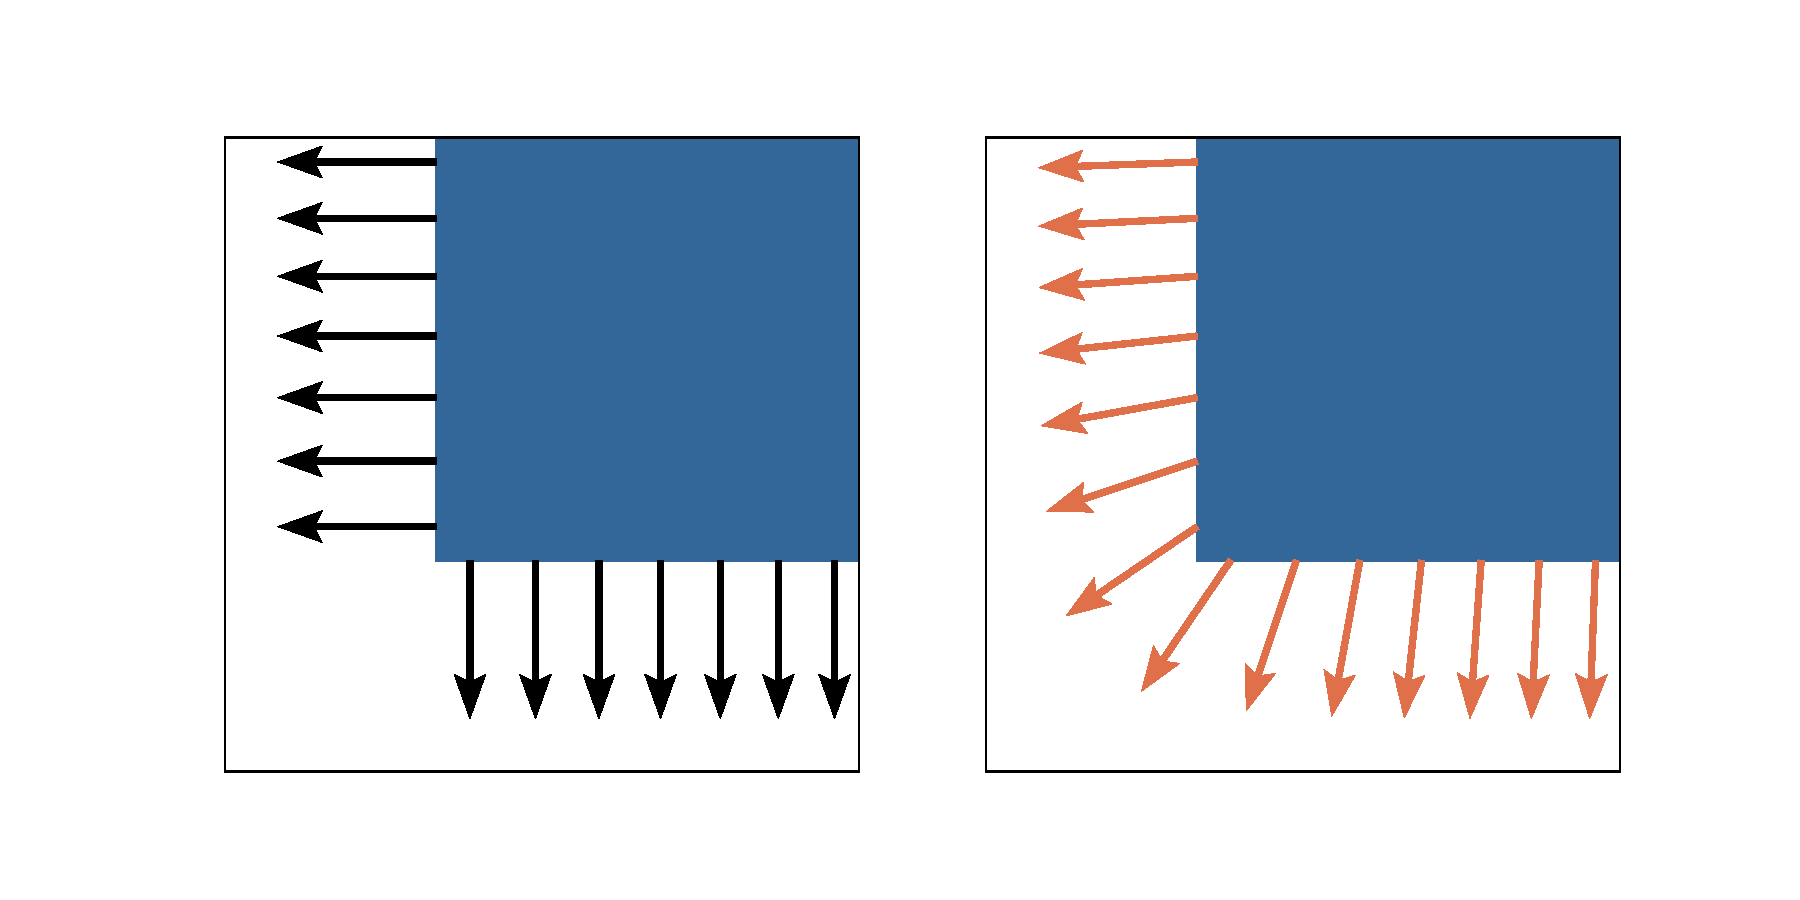
\includegraphics[width=.8\linewidth]{figures/dcol_normals_v2.pdf}

        \definecolor{CUST}{HTML}{E0704A}
        \begin{tikzpicture}
            % \draw[black, thick] (0,0.5) rectangle (6, 1);

            \draw[black, line width=2pt] (-3.7, 1.77) -- (-3.0, 1.77);
            \node[anchor=west] at (-2.8, 1.8) {$\kappa=0$};

            \draw[CUST, line width=2pt] (1.3, 1.77) -- (2.0, 1.77);
            \node[anchor=west] at (2.2, 1.8) {$\kappa=0.01$};
        \end{tikzpicture}
        \caption{Contact normal vectors from an optimization-based differentiable collision detection routine with and without relaxed differentiation. With no relaxation ($\kappa=0$), the direction of the contact normal switches immediately as the closest point moves from one face to another. When relaxed gradients are used ($\kappa=0.01$), the contact normal smoothly transitions between the faces.}
        \label{qpax:fig:dcol}
    \end{figure}
Collision detection between convex shapes can be formulated as a convex optimization problem, both in terms of the closest point between shapes \cite{gilbert1988}, and in terms of the minimum scale factor \cite{tracy2023b}. For the former, we introduce two points in a world frame $p_i \in \R{3}$, and two polytopes described with $A_i p_i \leq b_i$. By constraining each point to be within a polytope, a QP is used to solve for the closest point between these two shapes,
\begin{mini}
    {p_1, p_2}{ \|p_1 - p_2\|_2^2}{\label{qpax:gjk}}{}
    \addConstraint{A_1 p_1}{\leq b_1}%{k = 1,\ldots,N-1}
    \addConstraint{A_2 p_2}{\leq b_2.}%{k = 1,\ldots,N-1}
\end{mini}
Using a differentiable QP solver, the gradient of the objective value with respect to the positions of the polytopes results in the contact normal vectors.

In this example, we examine collision detection between two squares and the behavior of these contact normals in the presence of sharp corners. As shown in Fig. \ref{qpax:fig:dcol}, the contact normals are evaluated at a strict $\kappa=0$ and a relaxed $\kappa=0.01$. In the case of $\kappa=0$, the contact normals are (correctly) exactly normal to the surface, and as soon as the closest point shifts from one face to the other, the contact normals immediately rotate $90^\circ$. While this is expected behavior, this discontinuity in the gradient can prove troublesome for simulation and control algorithms that rely on these contact normals not changing too quickly. Alternatively, with a relaxed $\kappa=0.01$, the contact normal smoothly rotates the 90 degrees as the face of the closest point changes. This is a result of the logarithmic barrier smoothing out the sharp corner, and allows for continuous and smooth gradients even in the presence of the discontinuity.
% The efficacy of this approach for collision-free motion planning is demonstrated in \cite{tracy2023b}, where collision constraints are represented with differentiable optimization problems.
\section{Conclusions}
In this paper, we outline shortcomings with existing differentiable optimization tools, namely the nonsmoothness of the gradients near inequality constraints and the inability to handle infeasible problems, and propose solutions to both of these problems. By relaxing the solution to an optimization problem from tight tolerances to an intentionally relaxed logarithmic barrier, unique and smooth gradients can be computed even from sharp edges in the feasible set. This relaxation is straightforward and leverages existing routines within existing primal-dual interior-point solvers. We also introduce an always-feasible quadratic program where hard constraints are converted into $\ell_1$-penalties, and devise a customized algorithm for solving problems of this form with limited added computational overhead. With both of these innovations, consistent and reliable smooth gradients are demonstrated in common robotic tasks where smoothness is a priority. Our fully differentiable and parallelizable solver written in JAX is available at \url{www.github.com/kevin-tracy/qpax}.
% \graphicspath{{cpeg1/}}


\chapter{Atmospheric Entry Guidance}
\label{sec:cpeg1}

As scientific and crewed payloads have more demanding goals, precise atmospheric entry guidance is playing an increasing role in mission success. State-of-the-art entry guidance algorithms are structured in a predictor-corrector framework, where a simulation is used to predict a trajectory, and corrections are then made to the control inputs.  These guidance methods are simple and effective, but current algorithms assume low lift-to-drag entry vehicles, are limited to only bank-angle control, and have a limited ability to guarantee the safety of the vehicle. We propose a new predictor-corrector entry guidance method that formulates the correction step as a convex optimization problem. This allows for more flexibility in specifying the vehicle's dynamics and control inputs, and the ability to explicitly handle safety constraints such as heating, pressure, and acceleration limits. We test the new algorithm in Mars entry scenarios similar to the Mars Science Laboratory with both bank-angle control and bank-angle plus angle-of-attack control, demonstrating both its performance and ability to generalize to future vehicle capabilities.

The contents of this chapter have been previously published at IEEE Aerospace Conference 2021 in \citet{tracy2022c}

%%%%%%%%%%%%%%%%%%%%%%%%%%%%%%%%%%%%%%
\section{Introduction}
%%%%%%%%%%%%%%%%%%%%%%%%%%%%%%%%%%%%%%
In 1971 the Soviet Union's Mars-2 spacecraft made history by entering the Martian atmosphere before impacting the surface.  Nine days later, an identical Mars-3 spacecraft performed the first soft-landing on the Martian surface, ushering in a new era in planetary exploration. NASA followed with successful Mars landings in 1976 with Viking 1 and 2 and has since then landed and operated multiple robotic systems on the Martian surface \cite{li2014}. 

Entry vehicle architectures can be divided into three broad categories \cite{li2014}: 1) Ballistic entry is an uncontrolled descent with drag as the only force, 2) unguided ballistic-lifting entry has an uncontrolled non-zero lift force, and 3) guided ballistic-lifting entry has some control over the vehicle's lift vector. Controlled entry guidance allows for the prioritization of landing locations with scientific merit instead of just those that minimize risk to the vehicle.

The Mars Science Laboratory (MSL) carrying the Curiosity rover touched down in 2012 as the first Mars entry vehicle with guided ballistic-lifting entry.  MSL had control over the vehicle bank angle during entry, enabling control of the direction of the lift vector within the lifting plane. While MSL dramatically reduced the size of the landing ellipse from over 100 km to 10 km, its guidance is still too coarse for pinpoint landings. By developing more performant entry guidance capabilities, entry vehicles could effectively place robotic or crewed landers in desirable science collection areas, including high altitude sites. 

% \section{Previous Work}
Much of the work on guidance for low lift-to-drag entry vehicles originated with the Apollo terminal guidance methods. These algorithms, as described in \cite{graves1972}, rely on control of the bank angle with simple switching manuevers to control the cross-range and down-range errors. Slightly modified versions have been developed for use with more recent Mars entry vehicles, such as in \cite{mendeck2014}.  Current research investigates the use of predictor-corrector algorithms \cite{brunner2012} to improve the landing accuracy. A popular predictor-corrector formulation that exhibits bank-angle switching behavior is the Fully Numerical Predictor-corrector Entry Guidance (FNPEG) algorithm \cite{lu2008}. In the baseline FNPEG algorithm, Newton's method is used to solve for a static bank-angle that satisfies a terminal downrange distance constraint, and the sign of the bank-angle is modulated to control crossrange errors \cite{lu2014}. Here, the prediction phase is used to generate gradients for the terminal constraint, and corrections are applied to the open-loop commanded bank-angle in an effort to satisfy these terminal constraints. This framework is simple and effective but requires significant added complexity for incorporation of safety constraints or changes to the vehicle control inputs.

Trajectory optimization for offline planning of entry vehicle trajectories has been explored in \cite{wang2016} and \cite{wang2018a}, where the nonconvex optimal control problem was solved by linearizing the nonlinear dynamics and constraints, solving a conic optimization problem with a trust region, and repeating until convergence. This successive-convexification method was used instead of standard NonLinear Programming (NLP) solvers, like SNOPT \cite{gill2005} or IPOPT \cite{wachter2006}, because it is able to directly handle second-order cone constraints instead of relying on local linear approximations. Optimal trajectories computed offline were then paired with an optimization-based tracking controller, as described in \cite{wang2016} and \cite{wang2018a}. While these formulations are able to stabilize a trajectory, there are no guarantees that safety constraints can be satisfied online. Also, the computational complexity of the trajectory-optimization formulation makes these methods intractable for real-time control onboard an entry vehicle.

The Convex Predictor-corrector Entry Guidance (CPEG) algorithm proposed in this paper combines ideas from trajectory optimization with the predictor-corrector guidance framework by solving a constrained optimization problem during the correction step.  First, the dynamics of the entry vehicle with the current control plan are simulated to a target altitude for a predicted trajectory. Next, the vehicle dynamics are linearized about the predicted trajectory and a convex trajectory optimization problem is solved that minimizes landing error. By solving for a correction using convex optimization, CPEG is able to reason about the full state and control history to inform the correction instead of just the final state.  This also allows for the vehicle's safety constraints, such as heating, pressure, and acceleration, to be explicitly included in the correction computation. Our specific contributions in this paper are:
\begin{enumerate}
    \item A general quasi-linear formulation of entry vehicle dynamics that is well-suited to numerical optimization.
    \vspace{8pt}
    \item A predictor-corrector entry guidance algorithm with a highly generalizable correction step utilizing convex optimization.
    \vspace{8pt}
    \item Customized trust regions and objective functions for entry vehicles with multiple control modalities. 
\end{enumerate}

The paper proceeds as follows: In Section \ref{sec:cpeg1:dynamics}, the classic Vinh entry vehicle dynamics are compared with a more modern Cartesian approach. In Section \ref{sec:cpeg1:trajopt}, the details of the full nonconvex trajectory optimization problem are discussed. In Section \ref{sec:cpeg1:cpeg}, the CPEG algorithm is derived. In Section \ref{sec:cpeg1:experiments}, CPEG is validated on entry vehicles with bank-angle control, as well as bank-angle and angle-of-attack control. Finally, Section \ref{sec:cpeg1:conclusion} outlines our conclusions and potential future research directions.


\section{Entry Vehicle Dynamics}
\label{sec:cpeg1:dynamics}

Despite much of the recent powered-descent guidance literature using Cartesian state representations, entry vehicles are still most often represented in spherical coordinates. In this section, the traditional entry vehicle dynamics denoted below as the ``Vinh'' model will be discussed, as well as an alternative Cartesian formulation. 

\subsection{The Vinh Model}
The classic Vinh model, presented in 1976 in \cite{busemann1976} and again a few years Later in Vinh's textbook \cite{vinh1980}, has been the standard method for simulating entry vehicles for the past 45 years. Parameterizing the entry vehicle in spherical coordinates, the state in the Vinh model contains familiar terms like latitude, longitude, and flight-path angle. Despite being highly nonlinear and prone to scaling issues, it is the most common dynamics model in the literature \cite{busemann1976,vinh1980,vinh2000,wang2018,wang2019a,lu2014,gallais2007}.

The dynamics in the Vinh model are calculated with the angle-of-attack, $\alpha$, bank-angle, $\sigma$, flight-path angle, $\gamma$, longitude, $\theta$, latitude, $\phi$, and heading angle, $\psi$. The resulting equations of motion over a planet that's rotating with a constant angular velocity $\Omega$ are,
\begin{align}
\dot{r}&=V \sin \gamma ,\label{eq:vin1}\\
\dot{\theta}&=V \cos \gamma \sin \psi /(r \cos \phi) ,\\
\dot{\phi}&=V \cos \gamma \cos \psi / r ,\\
\dot{V}&=-D-\sin \gamma / r^{2} +\Omega^{2} r \cos \phi\sin \gamma \cos \phi   -\Omega^{2} r \cos \phi \cos \gamma \sin \phi \cos \psi  ,\\
\dot{\gamma}&=L \cos \sigma / V+\left(V^{2}-1 / r\right) \cos \gamma /(V r) +2 \Omega \cos \phi \sin \psi +\Omega^{2} r \cos \phi\cos \gamma \cos \phi / V   
 \\ & \quad \quad + \Omega^{2} r \cos \phi\sin \gamma \sin \phi \cos \psi / V , \\
\dot{\psi}&=L \sin \sigma /(V \cos \gamma)+V \cos \gamma \sin \psi \tan \phi / r 
 -2 \Omega(\tan \gamma \cos \psi \cos \phi-\sin \phi) \\ 
  & \quad \quad +\Omega^{2} r \sin \phi \cos \phi \sin \psi /(V \cos \gamma) , \label{eq:vin6}
\end{align}
where $r$ is the normalized radial distance from the center of the planet, $V$ is the normalized planet-relative velocity, and L and D are the magnitudes of the lift and drag accelerations. 

This model is highly nonlinear in both the state and the control, even when the planetary motion is ignored. While the planet's angular velocity is assumed to be constant, its inclusion in the dynamics still contributes significant nonlinearities. Because of this, much of the literature ignores the planet's angular velocity \cite{wang2016}. There are also scaling issues present if these equations are naively implemented. Since $r$ and $V$ are not angles, they are usually of a much larger magnitude than the rest of the state. This can lead to poor accuracy in variable time-step integrators, as well as ill-conditioning in numerical trajectory optimization.

\subsection{Cartesian Entry Dynamics}
We have found that entry vehicle dynamics are both simpler to derive and numerically better-conditioned when represented in standard Cartesian coordinates instead of the spherical coordinates used in the Vinh formulation. This state representation is popular with the powered-descent guidance community, albeit without any aerodynamic forces in the dynamics \cite{blackmore2012, acikmese2007, acikmese2013}.

We assume a planet-fixed frame $P$ is aligned with an inertial frame $N$ along the $z$ axis. The planet spins with angular velocity $\omega \in {\mathbb{R}}^3$ in the positive $z$ direction, making the velocity of the entry vehicle the following:
\begin{align}
{}^P v  &= {}^N v  -    \omega  \times r, \label{eq:pv}
\end{align}
where $^Nv \in {\mathbb{R}}^3$ is the inertial velocity, $^Pv \in {\mathbb{R}}^3$ is the planet relative velocity, and $r \in {\mathbb{R}}^3$ is the position of the entry vehicle in the planet frame. This expression can be differentiated once more to provide the relationship between the inertial and planet-relative accelerations:
\begin{align}
{}^P a &=   {}^{N} a -       2( \omega \times {}^P v )                          -   \omega  \times (\omega \times r) .\label{eq:Pa}
\end{align}
The state of the entry vehicle can be parameterized with the planet-relative position vector $r$, and planet relative velocity ${}^P v$ denoted as just $v$, both expressed in the coordinates of the planet frame. The Cartesian dynamics can now be written in state space as,
\begin{align}
    {\begin{bmatrix} v \\ a \end{bmatrix}} &= \begin{bmatrix} 0 & I \\ -[\omega \times]^2 & -2[\omega \times] \end{bmatrix}\begin{bmatrix}r \\v  \end{bmatrix} + \begin{bmatrix} 0 \\  a_{g} + a_{D} + a_{L} \end{bmatrix},\label{eq:dynamics}
\end{align}
where $[\omega \times]$ is the skew-symmetric cross product matrix,
\begin{align}
    [\omega \times ] &= \begin{bmatrix} 0 &-\omega_3 &\omega_2 \\ 
                                     \omega_3 &0 & -\omega_1 \\ 
                                     -\omega_2 & \omega_1 & 0 \end{bmatrix}.
\end{align}
One of the main benefits of the dynamics in equation \eqref{eq:dynamics} is the linear kinematics. This means that linear approximations of the relationship between position and velocity are exact, and the only nonlinearities present are in the accelerations. The gravitational acceleration in the direction of the planet's center is expressed assuming simple spherical gravity:
\begin{align}
    a_g &= -\frac{\mu}{\|r\|^3}r,
\end{align}
 where $\mu \in \mathbb{R}$ is the standard gravitational constant for the given planet. The acceleration caused by the drag force is in the direction opposing velocity, and is calculated as,
\begin{align}
    a_D &= - \frac{1}{2m}\rho A C_d \|v\| v,
\end{align}
where $m \in \mathbb{R}$ is the mass of the entry vehicle, $\rho \in \mathbb{R}$ is the atmospheric density, $A \in \mathbb{R}$ is the aerodynamic reference area, and $C_d \in \mathbb{R}$ is the coefficient of drag.  In this work, the atmospheric density $\rho \in \mathbb{R}$ will be represented by a piecewise exponential function \cite{gallais2007}.

\begin{figure}[t]
    \centering
    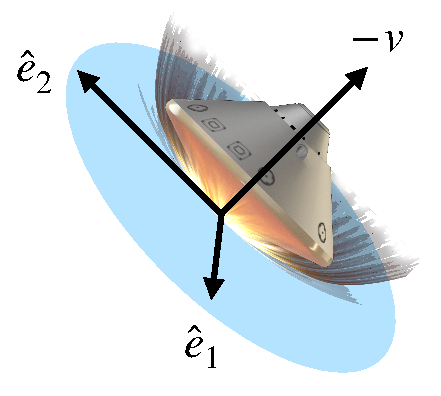
\includegraphics[width = 2in]{burn.pdf}
    \caption{The $E$ frame is fixed to the entry vehicle, with $\hat{e}_1$ in the direction of the specific angular momentum vector, and $\hat{e}_2 = \hat{v} \times \hat{e}_1$. When defined in this frame, the lift vector can be expressed using only $\hat{e}_1$ and $\hat{e}_2$.}
    \label{fig:eframe}
\end{figure}

For the description of the lift acceleration, a reference frame is defined that describes a plane about the entry vehicle that is orthogonal to the velocity vector.  This two-dimensional frame, referred to as the $E$ frame and depicted in Fig. \ref{fig:eframe}, has two basis vectors described by the following:
\begin{align}
    \hat{e}_1 &=  \frac{r \times v}{\|r \times v\|}, \\ 
    \hat{e}_2 &= \frac{v \times \hat{e}_1}{\| v \times \hat{e}_1 \|} .
\end{align}
The magnitude of the lift vector is calculated as,
\begin{align}
    \|L\| &= \frac{1}{2m} C_L \rho(r) A \|v\|^2,
\end{align}
where $C_L \in \mathbb{R}$ is the coefficient of lift. In the case where the entry vehicle only has control over the bank-angle, the resulting lift acceleration can be described by the magnitude of the lift and the bank-angle:
\begin{align}
    a_L &= \|L\|(\sin(\sigma)\hat{e}_1 + \cos(\sigma)\hat{e}_2). \label{eq:bao}
\end{align}
 In the case where the entry vehicle can control both the angle-of-attack as well as the bank-angle, the lift vector can be written as,
\begin{align}
    a_L &= \|L\|(\ell_1\hat{e}_1 + \ell_2\hat{e}_2), \label{eq:fl}
\end{align}
subject to the constraint $||\ell_1^2 + \ell_2^2|| \leq 1$.
Here the lift acceleration is a linear function of the control inputs, which is a key feature when this model is linearized in an optimization problem. Both the Vinh model and the Cartesian model are nonlinear, but the Cartesian model behaves significantly better under linearization, making it a far better candidate for trajectory optimization.


\subsection{State and Control Definitions}
In the case where only the bank-angle is controlled, the state is augmented with the bank-angle, and the sole control input is the derivative of this bank-angle with respect to time. This allows for cost functions that specify desired behavior for the derivative of the bank-angle, with the state and control as the following:
\begin{align}
x &= \begin{bmatrix} r^T & v^T & \sigma \end{bmatrix} ,\\ 
u &= \dot{\sigma}.
\end{align}
These dynamics are now in control-affine form with linear kinematics.  For the case with actuation of both the bank angle and angle-of-attack, the state and control are the following:
\begin{align}
x &= \begin{bmatrix} r^T & v^T \end{bmatrix}^T ,\\ 
u &= \begin{bmatrix} \ell_1 & \ell_2 \end{bmatrix}^T,
\end{align}
where $\ell_1$ and $\ell_2$ were defined in \eqref{eq:fl}. 
\section{Trajectory Optimization}
\label{sec:cpeg1:trajopt}
Feedback control laws for entry vehicles suffer in performance due to the severe underactuation of the vehicle. This is, in part, due to the fact that an entry vehicle has very limited ability to speed up or slow down in the along-track direction. To deal with this, it makes more sense to solve the guidance problem with a holistic planning approach, one that can reason about this limited control authority and plan for it. Therefore, we pose this problem as a trajectory optimization problem, where a locally optimal state trajectory and control plan can be solved for numerically.
%  \subsection{Reachable Set}
%  \todo{i kinda want to delete this section}
%  Given a bank-angle with a maximum angle-of-attack, the entry vehicle is able to control its final landing spot for the parachute deployment. To validate the dynamics model and view the possible places that the entry vehicle could deploy the parachute given this maximum allowable angle-of-attack, a set of simulations were run such that all of the possible bank-angles were sampled. The resulting plot is available in figure \ref{fig:reachable_set}, and is also known as the "landing footprint". This plot demonstrates that the entry vehicle does not have full controllabilty of the state and can't stabilize about a given trajectory, but it is able to fully articulate the spot in which the vehicle reaches an altitude of 10 km for the parachute deployment. This is critical because the objective of this control law is not to drive the state to a goal state at a goal time, but rather simply control the point in which the parachute system is deployed. 
% \begin{figure}
%     \centering
%     \includegraphics{tikz_figz/footprint.tikz}
%     \caption{Visualized reachable set for entry vehicle trajectories with only bank-angle control. Presented is a top view of 100 trajectories with varying bank-angle, each trajectory terminates at an altitude of 10 km.}
%     \label{fig:reachable_set}
% \end{figure}
 \subsection{Safety Constraints}
 Three key vehicle safety constraints --- heating, pressure, and acceleration --- are most dependent on the atmospheric density. Unfortunately, this is also the part of the environment in which there is the largest amount of uncertainty. The atmospheric density is often only known to roughly within a factor of two, with even less known about the wind conditions \cite{gallais2007}.
 
 The heating constraint has to do with the max allowable heat rate that the ablative heat shield can withstand \cite{edquist2007}. This is measured in power per square centimeter, and it is expressed as the following:
 \begin{align}
     \dot{Q} = k_q \sqrt{\rho}V^{3.15} \leq \dot{Q}_{max}. \label{eq:con_heat}
 \end{align} 
 This function is nonlinear but can be locally approximated with linear functions during the correction step.  The next safety constraint is the maximum dynamic pressure on the entry vehicle, which is expressed as the following:
 \begin{align}
     q = .5 \rho V^2 \leq q_{max}.\label{eq:con_press}
 \end{align}
 The last safety constraint is the maximum allowable normal load, which is the total aerodynamic force on the entry vehicle. This is expressed as a norm of the lift and drag forces:
 \begin{align}
     a = \sqrt{\|L\|^2 + \|D\|^2} \leq a_{max}.\label{eq:con_load}
 \end{align}
\subsection{Full Nonconvex Formulation}

In order to formulate a convex correction problem, we first consider the full nonlinear non-convex problem. First, the dynamics described in equation \eqref{eq:dynamics} are discretized with an explicit integrator like the classic fourth-order Runge-Kutta method \cite{montenbruck2002}, giving a discrete-time dynamics model of the form,
\begin{align} \label{eq: discrete-dynamics}
    x_{k+1} &= f(x_k,u_k,\Delta t_k).
\end{align}
No assumptions have been made about the control configuration in this dynamics model: it can account for either bank-angle-only or bank-angle plus angle-of-attack control. The full nonlinear trajectory optimization problem has the form,
% \begin{mini!} \label{nlp}
% {x,u,\Delta t}{x}{}{}
% %   {x,u,\Delta t}{\ell_N(x_N, u_N)+ \sum_{k=1}^{N-1}\ell_k(x_k, u_k) }{}{}
% %   \addConstraint{x_{k+1}}{= f(x_k,u_k,\Delta t_k),}{\forall k}
% %   \addConstraint{g_k(x_k, u_k)}{\leq 0,}{\forall k}
% %   \addConstraint{\Delta t_{min} \leq \Delta t_k }{\leq \Delta t_{max} }{\forall k}
% %   \addConstraint{x_N}{=x_{goal}}{},
% \end{mini!}
\begin{mini}<b>
  {x,u,\Delta t}{\ell_N(x_N, u_N)+ \sum _{k=1}^{N-1}\ell_k(x_k, u_k) }{}{}
  \addConstraint{x_{k+1}}{= f(x_k,u_k,\Delta t_k)}{\forall k} \labelOP{nlp}%\tag{test}
  \addConstraint{g_k(x_k, u_k)}{\leq 0}{\forall k} 
  \addConstraint{\Delta t_{min} }{\leq \Delta t_k \leq \Delta t_{max} }{\forall k}
  \addConstraint{x_N}{=x_{goal}}{},
 \end{mini}
 where safety constraints \eqref{eq:con_heat}---\eqref{eq:con_load} are included in the inequality constraint function $g_k(x_k, u_k)$. Note that this is a free-final-time problem in which the $\Delta t_k$ are decision variables in addition to the states and controls. This is necessary due to the inability of the entry vehicle to reach its goal state at an arbitrarily specified time. Problem \eqref{nlp} is nonconvex due to both the nonlinear dynamics, as well as the variable time between knot points. It is worth noting that, even with linear continuous-time dynamics, the discrete-time dynamics constraints \eqref{eq: discrete-dynamics} become nonlinear when the time step is made to be a decision variable.
 %This time step variable is bounded between two positive values to ensure the dynamics progress forward, and the dynamics don't take larger steps than is appropriate given the accuracy of the integrator. 
 
 Trajectory optimization problems like \eqref{nlp} can be solved with a variety of methods. One standard approach is to use an off-the-shelf NLP solver like IPOPT \cite{wachter2006} or SNOPT \cite{gill2005}. Alternatively, more specialized trajectory optimizers like ALTRO can be used \cite{howell2019,jackson2021}.  While computationally tractable using one of the described methods, the nonconvexity of the problem means there are no available guarantees for the quality of the solution or convergence of the solver. As a result, running nonconvex trajectory optimization onboard safety-critical aerospace systems is unpopular, explaining the prevalence of simpler heritage methods for entry guidance. 

 \section{Convex Predictor-corrector}
\label{sec:cpeg1:cpeg}
CPEG combines ideas from numerical trajectory optimization with the classic predictor-corrector guidance framework: It uses a prediction step, in which the vehicle dynamics are simulated until a target altitude is reached, combined with a corrector step that is based on solving a local convex approximation of a nonlinear trajectory optimization problem to steer the vehicle to the desired target. These steps are then repeated until convergence is achieved. This section provides a detailed derivation of the CPEG algorithm.

\subsection{Prediction and Dynamics Linearization}

In the first stage of CPEG, the dynamics of the entry vehicle are simulated with a standard Runge-Kutta method using the current nominal control trajectory, $\bar{U}$, until a target altitude is reached. We denote this predicted trajectory by $\bar{X}$. After the prediction step, the discrete-time nonlinear dynamics are approximated using a first-order Taylor series,
\begin{align}
    \bar{x}_{k+1} + \delta x_{k+1} \approx f(\bar{x}_k,\bar{u}_k) + A_k \delta x_k + B_k \delta u_k,
\end{align}
where $A_k$ and $B_k$ are the following Jacobians,
\begin{align}
    A_k &= \frac{\partial f(x_k,u_k,\Delta t_k)}{\partial x_k} \bigg\rvert _{\bar{x}_k,\bar{u}_k}, \label{jacob1}\\
    B_k &= \frac{\partial f(x_k,u_k,\Delta t_k)}{\partial u_k}\bigg\rvert _{\bar{x}_k,\bar{u}_k}. \label{jacob2}
\end{align}
Subtracting the dynamics of the reference trajectory from both sides, the local linear dynamics of trajectory corrections can be written as:
\begin{align}
    \delta x_{k+1} = A_k \delta x_k + B_k \delta u_k.\label{eq:linmod}
\end{align}
A crucial distinction between CPEG and sequential convexification methods \cite{wang2016,malyuta2021,mao2019}, is that trajectory iterates are always dynamically feasible, thanks to the prediction step. This eliminates the possibility of inconsistent linearizations of the dynamics constraints \cite{nocedal2006}, in which no feasible correction trajectory exists. Specifically, there is always a trivial solution to \eqref{eq:linmod} of all zeros for $\delta x$ and $\delta u$.

\subsection{Cost Function}
The cost function used in CPEG is comprised of a term that penalizes the miss distance from the target and a term that penalizes specified control behaviors. For the penalty on miss distance, putting a naive quadratic cost on the error between the final position and the desired position is inappropriate since it also penalizes altitude errors. Instead, only the position error projected onto the landing plane is penalized, effectively ignoring altitude error. Since the altitude target is implicitly satisfied during the prediction step, this allows for the correction to only apply changes to the control plan that minimize the projected miss distance. The cost function for this projected miss distance is the following:
\begin{align}
\ell_{miss}(\delta X,\delta U) &= \|W( r_N + \delta r_N - r_{goal})\|_2^2 ,\label{eq:miss}
\end{align}
where $r_N \in {\mathbb{R}}^3$ is the  final position in the reference trajectory, $\delta r_N \in {\mathbb{R}}^3$ is the correction computed for this position, and $r_{goal} \in {\mathbb{R}}^3$ is the desired final position for parachute deployment. To project this error onto the landing plane, we define following projection matrix, 
\begin{align}
W &= I - pp^T,
\end{align}
where $p$ is the unit vector normal to the planetary surface at the target position:
\begin{align}
p &= \frac{r_{goal}}{\|r_{goal}\|}.
\end{align}
The second part of the cost function seeks to shape the control behavior. In the case of bank-angle control, we consider two different control cost functions that produce qualitatively different behavior:
\begin{align}
    \ell_{\sigma,L1}(\delta U) &= \lambda \|\dot{\sigma_k}\|_1, \label{eq:bankl1}
\end{align}
and
\begin{align}
    \ell_{\sigma,quad}(\delta U) &= \lambda \dot{\sigma_k}^2, \label{eq:bankl2}
\end{align}
where $\lambda$ is a scalar tuning parameter. The first cost function \eqref{eq:bankl1} penalizes the L1 norm of the derivative of the bank-angle, resulting in bank-angle trajectories with a minimum number of discrete switches. The second cost function \eqref{eq:bankl2} penalizes the square of the bank-angle derivative, resulting in smooth bank-angle trajectories. For the bank-angle plus angle-of-attack case, as described in \eqref{eq:fl}, we apply a simple quadratic cost to the norm of the controlled lift vector, effectively penalizing high angles of attack:
\begin{align}
    \ell_{\sigma \alpha}(\delta U) &= \lambda \|u_k\|_2^2. \label{eq:baoa_cost}
\end{align}
\subsection{Constraints}
Of the three nonlinear safety constraints, two can be linearized, and the third can be converted to a conservative convex relaxation. For the heating and dynamic pressure constraints \eqref{eq:con_heat}--\eqref{eq:con_press}, a Taylor expansion of each is formed, approximating the constraint to first-order. From here, a linearized inequality constraint can be directly included in the convex correction problem. For these constraints, the linearized versions are:
\begin{align}
 [\nabla \dot{Q}(\bar{x}_k)]^T \delta x_k &\leq \dot{Q}_{max} - \dot{Q}(\bar{x}_k), \label{eq:lincon_heat}\\ 
  [\nabla {q}(\bar{x}_k)]^T \delta {x}_k &\leq {q}_{max} - {q}(\bar{x}_k). \label{eq:lincon_press}
\end{align}
The acceleration loading constraint \eqref{eq:con_load} is nonlinear, but a conservative convex relaxation can be derived in the form of a second-order cone constraint. First, the kinematics for the velocity can be conservatively approximated as the following:
\begin{align}
v_{k+1} &= v_k + a_k \Delta t, \\ 
a_k &= \frac{v_{k+1} - v_k}{\Delta t}, \\
a_k &=  \frac{\bar{v}_{k+1} + \delta v_{k+1} - \bar{v}_k - \delta v_k}{\Delta t}.
\end{align}
The maximum loading constraint can then be re-written as,
\begin{align}
% \|a_k\|_2 = \frac{1}{\Delta t} \|\bar{v}_{k+1} + \delta v_{k+1} - \bar{v}_k - \delta v_k\| &\leq a_{max} \\
 \|\bar{v}_{k+1} + \delta v_{k+1} - \bar{v}_k - \delta v_k\| &\leq  \Delta t \cdot a_{max}, \label{eq:lincon_accel}
\end{align}
which is in the form of a convex second-order cone, and can be directly incorporated into the correction problem.

The three  safety constraints from equations \eqref{eq:lincon_heat}, \eqref{eq:lincon_press}, and \eqref{eq:lincon_accel}, are stacked into a generic safety constraint function, 
\begin{align}
g_{safety}(\delta x_k, \delta u_k) &\leq 0 . 
\end{align}
\subsection{Trust Region}
To ensure that corrections are sufficiently small that the dynamics linearizations and constraint approximations remain accurate, a trust-region constraint is added to the convex correction problem. While standard trust-region methods apply norm constraints to $\delta  X$ and $\delta U$ \cite{nocedal2006}, insight into the entry guidance problem enables a more tailored approach. 

The quality of the linearization presented in \eqref{eq:linmod} is highly accurate for approximating the vehicle kinematics, gravity, and atmospheric drag, but is much less accurate when applied to the bank-angle in the bank-angle-only control case. Therefore, we design a trust region that restricts corrections to the bank-angle, $\delta \sigma_k$, given the known accuracy of small-angle approximations but allows large corrections to the other states. This approach also allows us to avoid the need to adapt trust regions inside the solver, enabling faster and more reliable convergence. We apply the following trust-region constraints to each corrector problem:
\begin{align}
\|\delta u_k\|_2 &\leq \delta u_{max}\\
|\delta \sigma_k | &\leq \delta \sigma_{max}
\end{align}
\subsection{Convex Corrector Problem}
For the case where the entry vehicle has control of only the bank-angle as described in \eqref{eq:bao}, the convex correction problem can be formulated as,
\begin{mini}
  {\delta X, \delta U}{\ell_{miss}(\delta X, \delta U) + \ell_{\sigma }(\delta U)}{\label{cpeg_boa}}{}
  \addConstraint{A_k \delta x_k + B_k \delta u_k}{=\delta x_{k+1}}{}
  \addConstraint{g_{safety}(\delta x_k, \delta u_k)}{\leq 0}{}
  \addConstraint{\|\delta u_k\|_2}{\leq \delta u_{max}}{}
  \addConstraint{|\delta \sigma_k |}{\leq \delta \sigma_{max},}{}
 \end{mini}
where the miss cost function is described in \eqref{eq:miss}, and the bank-angle cost function can be either \eqref{eq:bankl1} or \eqref{eq:bankl2}.

For the case where the entry vehicle has control over both bank-angle and angle-of-attack as described in \eqref{eq:fl}, the convex correction problem can be posed as:
\begin{mini}
  {\delta X, \delta U}{\ell_{miss}(\delta X, \delta U) + \ell_{\sigma \alpha}(\delta U)}{\label{cpeg_fl}}{}
  \addConstraint{A_k \delta x_k + B_k \delta u_k}{=\delta x_{k+1}}{}
  \addConstraint{g_{safety}(\delta x_k, \delta u_k)}{\leq 0}{}
  \addConstraint{\|u_k + \delta u_k\|_2}{\leq 1.}{} 
 \end{mini}
%A key difference here is that there is now a unit norm constraint on $u + \delta u$, ensuring the normalized lift control input does not exceed the maximum allowable lift.

These problems can be solved quickly and reliably by standard conic solvers such as Mosek \cite{mosekaps2014}, COSMO \cite{garstka2020}, and ECOS \cite{domahidi2013}.
%The trust region constraints ensure that the solution to this problem is within a reasonable region of linearization, allowing for the correction to be applied to the control plan with confidence.
 \subsection{CPEG Algorithm}
 The full CPEG algorithm is detailed in algorithm \ref{alg:flight}. The inputs to CPEG are the current position and the current control plan. From here, the dynamics of the entry vehicle are simulated until parachute deployment with the current control plan. This predicted trajectory is then discretized and linearized, resulting in dynamics Jacobians $A_k$ and $B_k$ (equations \eqref{jacob1}-\eqref{jacob2}). From here, the convex correction problem is posed given the control configuration and cost strategy. This convex optimization problem is solved, and the correction $\delta U$ is used to correct the control plan. The prediction-correction steps are repeated until the norm of the correction being made to the control plan is below a specified tolerance. 
  \begin{algorithm} 
	\begin{algorithmic}[1]
		\caption{CPEG Algorithm}\label{alg:flight}
		\State \textbf{input} $x_0$, U  \Comment{nominal control plan}
		\While{$\|\delta U\| > $ tolerance}
    		\State $\Bar{X}, \Bar{U} = \text{simulate}(x_0,U)$ \Comment{predict trajectory}
    		\State $A,B = \text{linearize}(\Bar{X}, \Bar{U})$ \Comment{linearize about prediction}
    		\State $\delta X,\delta U = \text{cvx}(\Bar{X}, \Bar{U}, A, B)$ \Comment{solve for correction} 
    	    \State $U \mathrel{+}= \delta U $ \Comment{correct control plan}
		\EndWhile
		\State \textbf{return} $U$ \Comment{return updated control plan}
	\end{algorithmic}
\end{algorithm}

\section{Numerical Experiments}
 \label{sec:cpeg1:experiments}
Parameters roughly matching those of the Mars Science Laboratory (MSL) \cite{mendeck2014} were used to test the CPEG algorithm. All scenarios begin at an altitude of $125$ km above the Martian surface with a Mars-relative velocity of 5.845 km/second. CPEG was implemented in the Julia programming language \cite{bezanson2017}, using the Convex.jl optimization modeling library \cite{udell2014}, and the Mosek \cite{mosekaps2014} and OSQP \cite{stellato} solvers. CPEG was validated on the following three cases:
\begin{itemize}
    \item Bank-angle control with L1 cost penalty, denoted $\sigma_{L1}$.
    \vspace{+2mm}
    \item Bank-angle control with quadratic penalty, denoted $\sigma_{2}$.
    \vspace{+2mm}
    \item Bank-angle plus angle-of-attack control, denoted $\sigma + \alpha$.
\end{itemize}
For the bank-angle cases, CPEG was arbitrarily initialized with a constant bank-angle of zero, with noise added to the bank-angle derivative. For the bank-angle plus angle-of-attack case, a similar approach was used, but noise was added to the normalized lift vector. The final converged trajectories for the three cases are shown in figures \ref{fig:allalt} and \ref{fig:allcrdr}. In all of the cases, CPEG was able to successfully guide the entry vehicle to the target point at the desired altitude.
\begin{figure}
    \centering
    \includegraphics{cpeg1/tikz/all_altdr.tikz}
    \caption{Altitude and downrange distance from the converged trajectories from CPEG on the three specified cases. The $\sigma_{L1}$ case is with bank-angle control and an L1 penalty on bank-angle derivative, $\sigma_{quad}$ is bank-angle only with a quadratic penalty on bank-angle derivative, and $\sigma + \alpha$ is control over both bank-angle and angle-of-attack. Due to the differences in control authority and cost function, all three converge on different trajectories that hit the target position at parachute deployment.}
    \label{fig:allalt}
\end{figure}
% \todo{Describe what the different cases are in all of the figure captions as well (i.e. spell out what the labels mean).}
\begin{figure}
    \centering
    \includegraphics{cpeg1/tikz/all_crdr.tikz}
    \caption{Crossrange and downrange trajectory data from the converged trajectories from CPEG on the three specified cases. The cases with only control over the bank-angle have to do a bank reversal to hit the target, whereas the case with control over bank-angle and angle-of-attack is able to leverage the full lift control to avoid the switching.}
    \label{fig:allcrdr}
\end{figure}
\subsection{Bank-Angle Control}
For the case where the entry vehicle has only bank-angle control, the convergence of CPEG can be observed in figures \ref{fig:l1alt} and \ref{fig:l1crdr} for the case with an L1 cost on the bank-angle derivative, and figures \ref{fig:l2alt} and \ref{fig:l2crdr} with a quadratic cost.  These plots show the output of the prediction step of CPEG, where the color of the predictions is blue for the first iteration of the algorithm and turns purple, then pink for later iterations.
\begin{figure}
    \centering
    \includegraphics{cpeg1/tikz/L1_altdr.tikz}
    \caption{Predicted entry vehicle trajectories for the bank-angle only L1 penalty case, as seen by the altitude and downrange data. As the iterates continue, the entry vehicle converges on a trajectory that reaches the target at the 10km altitude mark.} 
    \label{fig:l1alt}
\end{figure}
\begin{figure}
    \centering
    \includegraphics{cpeg1/tikz/L1_crdr.tikz}
    \caption{Predicted entry vehicle trajectories for the bank-angle only L1 penalty case, as seen by the crossrange and downrange data.}
    \label{fig:l1crdr}
\end{figure}
  \begin{figure}
    \centering
    \includegraphics{cpeg1/tikz/L2_altdr.tikz}
    \caption{Predicted entry vehicle trajectories for the bank-angle only quadratic penalty case, as seen by the altitude and downrange data. The}
    \label{fig:l2alt}
\end{figure}
\begin{figure}
    \centering
    \includegraphics{cpeg1/tikz/L2_crdr.tikz}
    \caption{Predicted entry vehicle trajectories for the bank-angle only quadratic penalty case, as seen by the crossrange and downrange data.}
    \label{fig:l2crdr}
\end{figure}
After convergence, the two bank-angle profiles that CPEG produced for the L1 and quadratic cost functions are shown in figure \ref{fig:banks}. The L1 cost on the derivative of the bank-angle encouraged sparsity in this derivative, resulting in a bank-angle profile that switches between constant bank-angles. For the case with a quadratic cost on the bank-angle derivative, the resulting bank-angle profile is smooth with no discrete switching behavior.
\begin{figure}
    \centering
    \includegraphics{cpeg1/tikz/banks.tikz}
    \caption{Bank-angle only control plans for both the L1 and quadratic cost cases. The L1 cost motivated a bang-bang switching style bank-angle profile. The quadratic cost resulted in a smooth and continuous bank-angle profile.}
    \label{fig:banks}
\end{figure}
\subsection{Bank-Angle and Angle-of-Attack Control}
As described by the dynamics in equation \eqref{eq:fl}, the control input for this case is the lift vector itself in the directions orthogonal to the velocity vector. This allows for manipulation of both the bank-angle and angle-of-attack and is guaranteed to be within the maximum allowable lift by the unit norm constraint in equation \eqref{cpeg_fl}. In this control case, the control input Jacobian is constant and independent of the nominal control plan, making the linearization significantly more accurate than the bank-angle-only case. As a result, the convergence of CPEG with bank-angle plus angle-of-attack control is significantly faster than with the bank-angle alone. The evolution of the predicted trajectories is shown in figures \ref{fig:flalt} and \ref{fig:flcrdr}, with the same coloring scheme as the bank-angle only section. After convergence, the control inputs were converted back into bank-angle and angle-of-attack and shown together in figure \ref{fig:flcontrols}.
\begin{figure}
    \centering
    \includegraphics{cpeg1/tikz/FL_altdr.tikz}
    \caption{Predicted entry vehicle trajectories for the bank-angle and angle-of-attack case, as seen by the altitude and downrange data.}
    \label{fig:flalt}
\end{figure}
\begin{figure}
    \centering
    \includegraphics{cpeg1/tikz/FL_crdr.tikz}
    \caption{Predicted entry vehicle trajectories for the bank-angle and angle-of-attack case, as seen by the crossrange and downrange data.}
    \label{fig:flcrdr}
\end{figure}
\begin{figure}
    \centering
    \includegraphics{cpeg1/tikz/fl_controls.tikz}
    \caption{Bank-angle and angle-of-attack profiles for the case where both angles are being controlled. CPEG was able to converge on this control plan in just three iterations.}
    \label{fig:flcontrols}
\end{figure}
\section{Conclusion}
\label{sec:cpeg1:conclusion}
This paper proposes an improved version of the classic predictor-corrector entry guidance scheme in which the correction step is formulated as a convex optimization problem. Two control strategies were tested with CPEG: bank-angle control, and bank-angle plus angle-of-attack modulation. For the bank-angle-only case, cost functions that penalized the derivative with an L1 cost and a quadratic cost were both demonstrated, resulting in dramatically different optimal bank-angle profiles. For the case with both bank-angle and angle-of-attack control, the quality of the dynamics linearization was accurate enough that CPEG was able to converge on an optimal trajectory in just a few iterations. An implementation of CPEG running all of the examples in this paper is available at \url{https://github.com/RoboticExplorationLab/EntryGuidance.jl}.


%%% Local Variables:
%%% coding: utf-8
%%% mode: latex
%%% TeX-engine: xetex
%%% TeX-master: "../thesis"
%%% End:
% \graphicspath{{cpeg2/}}


\chapter{Robust Entry Guidance with Atmospheric Adaptation}
\label{sec:cpeg2}

Robust atmospheric entry guidance for blunt-body entry vehicles with bank angle modulation is achieved by combining online atmospheric density estimation with an updated version of the Convex Predictor-corrector Entry Guidance (CPEG) algorithm. During atmospheric entry, a square-root Extended Kalman Filter is used to estimate a ratio between the density of the experienced atmosphere with that of an approximate model, which is spline-fit based on MarsGRAM perturbed data. The information from this filter is used to modify the approximate model used by the guidance algorithm. The proposed update to CPEG includes time as a decision variable, dramatically improving the robustness of the algorithm. CPEG predicts the trajectory at each control call with a nonlinear simulation followed by a single convex trajectory optimization problem that updates the commanded bank angle derivative. The robustness and performance of this estimator and controller guidance architecture are demonstrated on a wide range of realistic Martian atmospheres and is able to achieve state-of-the-art accuracy with respect to altitude-triggered parachute deployment.

The contents of this chapter have been previously published at IEEE Aerospace Conference 2021 in \citet{tracy2023}


\section{Introduction}
Entry into the Martian atmosphere refers to the phase of Entry, Descent, and Landing (EDL) that occurs between the point at which the hypersonic entry vehicle first interfaces with the planet’s sensible atmosphere and the point at which the supersonic parachute is deployed. It is during this portion of the EDL that the vehicle is subjected to the most demanding flight conditions, during which both peak acceleration and peak heating are experienced \cite{way2007}. Large uncertainties in models of the Martian atmospheric environment make entry guidance challenging, and significantly degrade landing accuracy, where the landing accuracy is the distance between the landing target site and the actual landing site. Actual atmospheric density can deviate from predictions by a factor of two or more \cite{justh2013}, requiring guidance laws to combat uncertainty with frequent re-planning and reliance on conservative initial entry conditions. These approaches ultimately reduce performance and limit the potential landing sites that can be accessed on Mars \cite{li2014}. To enable precision landing, which could potentially increase the number of reachable sites of high scientific interest, we propose a new approach to entry guidance that can strategically account for and reduce the atmospheric model uncertainty during guided entry.
\begin{figure}[h!]
\centering
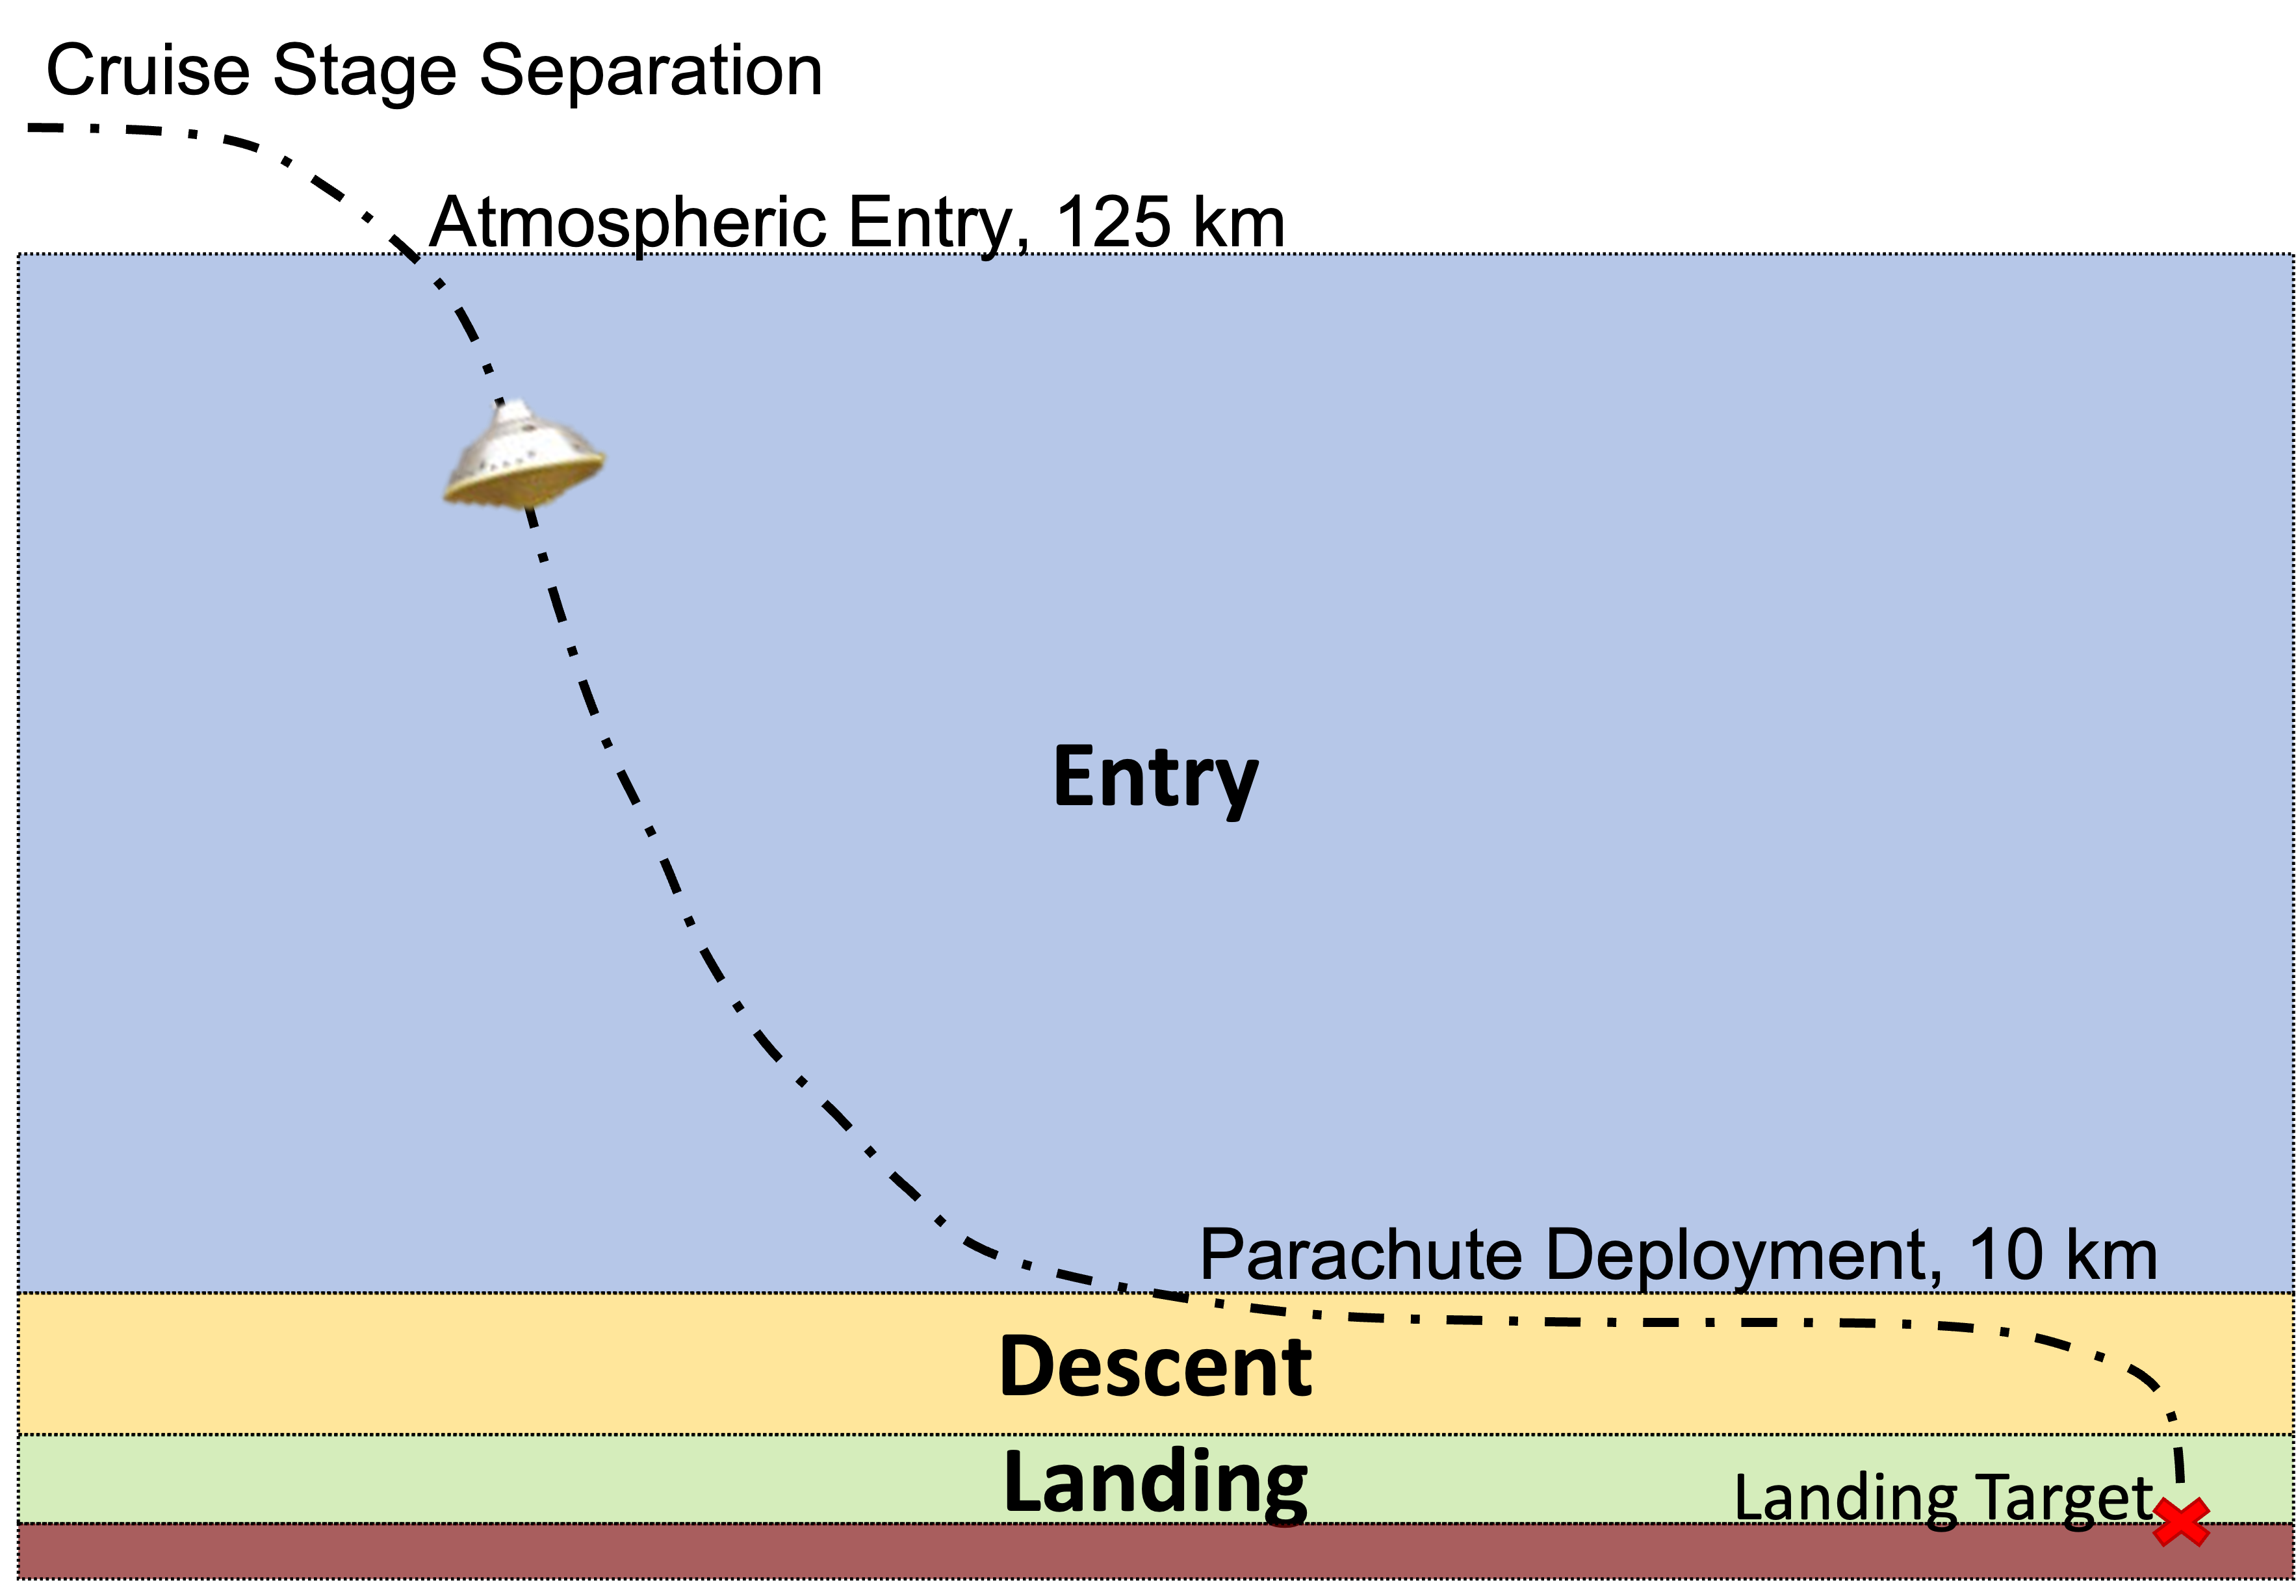
\includegraphics[width=0.5\linewidth]{entry.png}
  \caption{Cartoon representation of entry, descent, and landing.}
  \label{fig:entry}
\end{figure}

In the last few decades, predictor-corrector guidance algorithms have become the state-of-the-art; these have offered steadily improving landing accuracy with modest computational costs. These methods, like PredGuid \cite{putnam2010,putnam2014} and FNPEG \cite{lu2014a}, predict the trajectory of the entry vehicle with a nonlinear simulation, then use derivative or ``sensitivity'' information from the simulation to improve or ``correct'' the control plan \cite{lu2008,brunner2008}. This predictor-corrector framework offers improved landing accuracy compared to Apollo-era entry guidance methods \cite{brunner2012a} while being relatively simple to implement with low computational complexity. However, a significant drawback of traditional predictor-corrector guidance methods is their inability to generate complex control policies; many such methods are restricted to solving for a static bank angle, which means that the initial bank angle control profile predicted for the whole entry phase is considered constant; however, only during the prediction and correction phase, the guidance uses independent downrange and crossrange control to determine when the sign of the bank angle should flip. This simplicity severely limits the sophistication of the guidance method, and the resulting performance can chatter with multiple aggressive bank angle switches. Another limitation of existing predictor-corrector guidance strategies is their inability to incorporate real-time information about the Martian atmosphere, which is the largest source of uncertainty in the vehicle's dynamics, for prediction and correction purposes. 

Recently, there has been a growing interest in trajectory optimization methods for open-loop entry guidance for both Earth and Mars. This approach, in which the guidance problem is formulated as a numerical optimization problem, enables algorithms that can reason about the dynamics of the vehicle and constraints like actuator limits, state bounds, and heating limits. These optimization problems can be solved by a variety of numerical methods. As an example, sequential convex programming, in which a non-convex optimization problem is iteratively convexified and solved until convergence, has recently become popular \cite{wang2016,wang2018,mao2019,szmuk2019,szmuk2020,malyuta2021}. Alternatively, the trajectory optimization problem can be converted into a nonlinear program \cite{betts2001} and solved by a variety of off-the-shelf solvers, like SNOPT \cite{gill2005} or Ipopt \cite{wachter2006}, or by a more specialized trajectory optimization solver like ALTRO \cite{howell2019, jackson2021b}. While these trajectory optimization guidance methods offer more sophisticated and performant control plans than classical predictor-corrector methods, they can be prohibitively complex to implement on resource-constrained flight computers, and are still unable to account for real-time information about the atmosphere. 

A middle ground between simple predictor-corrector guidance schemes and offline trajectory optimization is the Convex Predictor-corrector Entry Guidance algorithm (CPEG) \cite{tracy2022a}. This method uses the same predictor-corrector framework as existing methods, but instead of solving for a simple static bank angle, it forms a convex trajectory optimization problem that solves for the correction to the nominal control plan. This approach enables the direct inclusion of any actuator or safety constraints and the ability to reason about complex control policies and the dynamics of the vehicle over the whole trajectory. By forming the convex trajectory optimization problem with a dynamics model linearized about the prediction rollout, the problem is guaranteed to always be feasible, and the convexity of the problem guarantees that an optimal solution can be computed in polynomial time \cite{boyd2004}. 

This work proposes an improvement to the CPEG algorithm that includes time as an optimization variable, allowing for the generation of trajectories with a free final time. This modification allows for significantly more flexibility when handling scenarios with multiple potentially successful control policies, since many trajectories can all be expressed using the same number of optimization variables. The absence of this feature in the original CPEG algorithm resulted in a lack of robustness when run online with significant model uncertainty. Additionally, this work directly addresses the main source of the uncertainty in the vehicle dynamics -- the atmospheric density -- by estimating information about the atmosphere online and including it in the approximate model used by CPEG. Our specific contributions include:
\begin{enumerate}
    \item A free-final-time extension of the Convex Predictor-corrector Entry Guidance algorithm
    \item An estimation architecture for atmospheric density and an atmospheric approximate model
    \item Validation of the combined controller and estimator on realistic density and wind dispersions from MarsGRAM \cite{justh2013}
\end{enumerate}

This paper proceeds by first describing the dynamics of the entry vehicle in Cartesian coordinates in Section \ref{sec:cpeg2:section3}, followed by the free-final-time version of CPEG in Section \ref{sec:cpeg2:section4}. The atmospheric density estimation approach is detailed in Section \ref{sec:cpeg2:section5}. Numerical experiments using Monte-Carlo sampling of atmospheric parameters from MarsGRAM are presented in Section \ref{sec:cpeg2:section6}. Finally, Section \ref{sec:cpeg2:section7} summarizes our conclusion.

\section{Entry Vehicle Dynamics}\label{sec:cpeg2:section3}
This work considers a blunt-body entry vehicle in the Martian atmosphere with the ability to modulate its bank angle $\sigma \in \R{}$. These entry vehicles are traditionally described and simulated in spherical coordinates using the “Vinh” model \cite{busemann1976,vinh1980,vinh2000,wang2018,wang2019a,lu2014a,gallais2007}. While this model is ubiquitous and well-studied, it suffers from numerical scaling issues due to the state vector including angles as well as distance and velocity, and is highly nonlinear in both the state and the control input. These shortcomings make optimization challenging and numerically unreliable. Alternatively, the state and dynamics of the entry vehicle can be equivalently described in a Mars-fixed Cartesian reference frame. This parametrization is more common in the powered-descent guidance literature \cite{blackmore2012, acikmese2007, acikmese2013}, and has much better numerical scaling, as well as linear kinematics, both of which make it a better fit for optimization-based control methods as detailed in \cite{tracy2022}. The dynamics of the entry vehicle with this state representation are the following:
\begin{align}
    \dot{r} &= v, \\ 
    \dot{v} &= a_L + a_D + a_g - 2 (\omega \times v) - \omega \times (\omega \times r).
\end{align}
% where $a_L \in \R{}$, $a_D \in \R{}$, and $a_g \in \R{}$ are, respectively, the accelerations due to lift, drag, and gravity, and $\omega \in \R{3}$ is the angular velocity of the planet in this Mars-fixed frame.  
The aerodynamic accelerations from lift and drag are dependent on the vehicle velocity relative to the atmosphere, including wind. The wind vector $w$ is expressed in the Mars-fixed frame, and the relative velocity is simply $v_{rel} = v + w$. The magnitude of the lift and drag accelerations can then be computed as follows:
\begin{align}
    L &= \frac{1}{2m} \rho A C_L \|v_{rel}\|^2, \\ 
    D &= \frac{1}{2m} \rho A C_D \|v_{rel}\|^2.
\end{align}
% where $A \in \R{}$ is the cross-sectional area of the vehicle, $C_L \in \R{}$ and $C_D \in \R{}$ are the coefficients of lift and drag respectively, $m \in \R{}$ is the mass of the vehicle, and $\rho$ is the atmospheric density. 
The hypersonic coefficients, $C_L$ and $C_D$ have been evaluated through the Newtonian flow theory for a blunted body, specifically: 
\begin{align}
    C_A &= (1-\sin{\delta}^4)  \dfrac{r_{nose}^2}{r_{base}^2} + (2\sin{\delta}^2 \cos{\alpha}^2 + \cos{\delta}^2 \sin{\alpha}^2)\left(1-\dfrac{r_{nose}^2}{r_{base}^2} \cos{\delta}^2\right),\\
    C_N &= \left(1-\dfrac{r_{nose}^2}{r_{base}^2} \cos{\delta}^2\right)\cos{\delta}^2\sin{2\alpha},\\
    C_L &= C_N\cos{\alpha}-C_A\sin{\alpha},\\
    C_D &= C_A\cos{\alpha}+C_N\sin{\alpha},
\end{align}
where $C_A$ is the axial force coefficient, $C_N$ is the normal force coefficient, $\delta$ is the cone angle of the blunted-cone vehicle,  $\alpha$ is the angle of attack, $r_{base}$ is the base radius, $r_{nose}$ is the nose radius of the hypersonic vehicle.
        
The direction of the drag acceleration is in the opposite direction of the relative velocity, expressed as:
\begin{align}
    a_D &= -D \frac{v_{rel}}{\|v_{rel}\|}.
\end{align}
The lift acceleration is directed using the bank angle $\sigma$, and is modeled and represented with two basis vectors $\hat{e}_1 \in \R{3}$ and $\hat{e}_2 \in \R{3}$, where together they span the plane orthogonal to the relative velocity of the vehicle in the atmosphere. These aerodynamic basis vectors are constructed as the following:
\begin{align}
    \hat{e}_1 &=  \frac{r \times v_{rel}}{\|r \times v_{rel}\|}, \\ 
    \hat{e}_2 &= \frac{v_{rel} \times \hat{e}_1}{\| v_{rel} \times \hat{e}_1 \|} .
\end{align}
Using these basis vectors, the lift acceleration can be computed as the following:
\begin{align}
    a_L &= L(\sin(\sigma) \hat{e}_1 + \cos(\sigma)\hat{e}_2).
\end{align}
The acceleration due to gravity can be calculated using any number of established methods ranging in fidelity from simple two-body gravity \cite{montenbruck2002}, to a more complex spherical harmonic expansion of the geopotential \cite{hirt2012,genova2016}. 

The largest amount of uncertainty in the dynamics of the entry vehicle comes from the atmosphere. Both the atmospheric density $\rho$, as well as the wind vector $w$ are highly uncertain. To visualize this uncertainty, Mars GRAM \cite{justh2013} was used to generate dispersions for these two parameters, which are shown in Fig. \ref{fig:mgdensity} and Fig. \ref{fig:mgwind}. A summary of the parameters used to run Mars GRAM is presented in Table \ref{tab:marsgram}. For the generation of atmospheric data points in highly perturbed environments, Mars GRAM not only uses random Monte Carlo samples that re-initialize the random number seed (NR1) for each sample but also has been set for different zoffsets, which are constant height offsets that modify the atmospheric density. Specifically, positive offsets increase density, while negative offsets decrease density. In addition, rpscale, the random perturbation scale was also set to the maximum, with increasing this factor intensifying the magnitude of the perturbation. The data have also been evaluated in the context of a global dust storm, through INTENS, which changes the dust storm intensity. 

\begin{table}[h!]
\centering
\caption{Mars GRAM nominal and dispersion parameters}
\begin{tabular}{cccc}
\hline \hline
Parameter & Value   & Parameter                                                                        & Value \\ \hline 
\begin{tabular}[c]{@{}c@{}}Initial Altitude, km\end{tabular} &
  125 &
  \begin{tabular}[c]{@{}c@{}}NR1\end{tabular} &
  {[}1,5001{]} \\
Date &
  6 August 2012 &
  \begin{tabular}[c]{@{}c@{}}zoffset, km\end{tabular} &
  \begin{tabular}[c]{@{}c@{}}Uniform Dist., {[}-3.25,3.25{]}\end{tabular} \\
Time      & 5:30:00 & \begin{tabular}[c]{@{}c@{}}rpscale\end{tabular} & 2     \\
\begin{tabular}[c]{@{}c@{}}Final Altitude, km\end{tabular} &
  10 &
  \begin{tabular}[c]{@{}c@{}}INTENS \end{tabular} &
  2\\
  \hline \hline
\end{tabular}
\label{tab:marsgram}
\end{table}

Since aerodynamic acceleration is the dominant term in the dynamics at the high speeds an entry vehicle experiences, the uncertainty in the atmospheric density results in a highly uncertain dynamics model. The uncertainty in the wind contributes to the model uncertainty, but less so than the density.  
\begin{figure}
    \centering
    \includegraphics{tikz/atmo_uncertainty/density_shaded.tikz}
    \caption{Dispersion of the atmospheric density as a function of altitude calculated with Mars GRAM.  The dynamics of the entry vehicle are heavily influenced by this density, and the dramatic uncertainty of this value motivates the need for more robust guidance schemes.}
    \label{fig:mgdensity}
\end{figure}
\begin{figure}
    \centering
    \includegraphics{tikz/atmo_uncertainty/wind_shaded.tikz}
    \caption{Dispersions of the east and north wind velocities in the Martian atmosphere as a function of altitude calculated with Mars GRAM. This range of atmospheric wind profiles is used in the Monte Carlo testing of the proposed entry guidance algorithm.}
    \label{fig:mgwind}
\end{figure}


\section{CPEG}\label{sec:cpeg2:section4}
Predictor-corrector guidance algorithms are a simple and effective way to control underactuated systems like the entry vehicle. These methods all share a general framework in which a nominal control policy is used to simulate a predicted trajectory, then a correction is made to the nominal control policy based on this prediction. Predictor-corrector methods have been the state of the art for entry guidance of blunt-body vehicles, but they are not without their shortcomings. Existing methods like FNPEG are only able to reason about simple static bank angle policies, and rely on independent crossrange and downrange logic to modulate the bank angle \cite{lu2008}. Alternatively, offline trajectory optimization allows for more complex control policies and the direct inclusion of constraints, but is significantly more expensive than predictor-corrector methods. A trajectory optimization problem in its most general form is the following,
\newpage
\begin{mini}<b>
  {x_{1:N},u_{1:N-1}}{\ell_N(x_N)+ \sum _{k=1}^{N-1}\ell_k(x_k, u_k)}{}{}
  \addConstraint{x_{k+1}= f(x_k,u_k)}{}{\quad k = 1 \ldots N-1} \labelOP{nlp}%\tag{test}
  \addConstraint{g_k(x_k, u_k)\leq 0 }{}{\quad k = 1 \ldots N-1} 
   \addConstraint{u_{min}\leq u_k \leq u_{max} }{}{\quad k = 1 \ldots N-1}
  \addConstraint{x_{min}\leq x_k \leq x_{max} }{}{\quad k = 1 \ldots N}
  % \addConstraint{\Delta t_{min} }{\leq \Delta t_k \leq \Delta t_{max} }{\forall k}
  % \addConstraint{x_N}{=x_{goal}}{},
 \end{mini}
where $x$ is the state, $u$ is the control, $\ell$ is the cost function, $f(x,u)$ is the discrete dynamics function, and $g(x,u)$ is a general constraint function. Problem \eqref{nlp} can be solved with a multitude of available trajectory optimization solvers, but they are prohibitively complex to run on board the entry vehicle. 
\subsection{Baseline CPEG}
The Convex Predictor-corrector Entry Guidance (CPEG) algorithm, introduced in \cite{tracy2022}, seeks to find a middle ground between simple predictor-corrector guidance methods and offline trajectory optimization. This is achieved by adopting the predictor-corrector framework, but solving a convex trajectory optimization problem for the correction instead of a simple update to a static bank angle like in FNPEG. This approach allows CPEG to reason about sophisticated control trajectories as well as the dynamics of the vehicle throughout the entirety of the trajectory. The convex optimization problem that makes up the correction portion of the algorithm is guaranteed to be feasible, and its optimum can be solved for at real-time rates \cite{mattingley2012}. 

In order for problem \eqref{nlp} to be convex, the cost and constraint functions must be convex. This means that problems with nonlinear dynamics, like the entry vehicle, must be approximated. We linearize the discrete dynamics function $f(x,u)$ about the predicted trajectory $(\bar{x},\bar{u})$:
\begin{align}
    \bar{x}_{k+1} + \delta x_{k+1} \approx f(\bar{x}_k,\bar{u}_k) + A_k \delta x_k + B_k \delta u_k, \label{taylor_series}
\end{align}
where $A_k$ and $B_k$ are the following Jacobians,
\begin{align}
    A_k &= \frac{\partial f(x_k,u_k)}{\partial x_k} \bigg\rvert _{\bar{x}_k,\bar{u}_k}, \label{jacob1}\\
    B_k &= \frac{\partial f(x_k,u_k)}{\partial u_k}\bigg\rvert _{\bar{x}_k,\bar{u}_k}. \label{jacob2}
\end{align}
Since the prediction was dynamically feasible, and $\bar{x}_{k+1} = f(\bar{x}_k,\bar{u}_k)$, equation \eqref{taylor_series} is reduced to
\begin{align}
    \delta x_{k+1} \approx   A_k \delta x_k + B_k \delta u_k.
\end{align}
From here, the convex correction problem is posed as,
% \todo{can we force this to be all on the same page? let's wait to fix everything before this point and if the problem is still there, we force it (G)}
\begin{mini}<b>
  {\delta x_{1:N},\delta u_{1:N-1}}{\ell_N(\bar{x}_N + \delta x_N)+ \sum _{k=1}^{N-1}\ell_k(\bar{x}_k + \delta x_k, \bar{u}_k + \delta u_k) }{}{}
  \addConstraint{\delta x_{k+1}=  A_k \delta x_k + B_k \delta u_k}{}{\quad k = 1 \ldots N-1} \labelOP{cto}%\tag{test}
  \addConstraint{g_k(\bar{x}_k + \delta x_k, \bar{u}_k + \delta u_k)\leq 0}{}{\quad k = 1 \ldots N-1} 
  \addConstraint{u_{min}\leq u_k \leq u_{max} }{}{\quad k = 1 \ldots N-1}
  \addConstraint{x_{min}\leq x_k \leq x_{max} }{}{\quad k = 1 \ldots N}
  \addConstraint{\delta u_{min}\leq \delta u_k \leq \delta u_{max} }{}{\quad k = 1 \ldots N-1}
  \addConstraint{\delta x_{min}\leq \delta x_k \leq \delta x_{max} }{}{\quad k = 1 \ldots N,}
  % \addConstraint{x_N}{=x_{goal}}{},
 \end{mini}
 where the bounds on $\delta x$ and $\delta u$ serve as a customizable trust region that ensures the step direction stays within a region of the state space where the linearization is accurate \cite{nocedal2006}. Since the linearization is evaluated about the dynamically feasible predicted trajectory, this optimization problem is guaranteed to have a feasible solution of all zeros for $\delta x$ and $\delta u$, eliminating one of the largest vulnerabilities in real-time optimization-based control. 

The full baseline CPEG algorithm is shown in Algorithm \ref{alg:flight}, where an initial condition and nominal control policy are used to simulate the entry vehicle until parachute deployment (the prediction), a linearized model is evaluated about this predicted trajectory, and a convex trajectory optimization problem \eqref{cto} is solved for the correction. 
  \begin{algorithm} [H]
	\begin{algorithmic}[1]
		\caption{CPEG Algorithm}\label{alg:flight}
		\State \textbf{function} $\operatorname{CEPG}(x_0, U$  \Comment{nominal control plan}
		% \While{$\|\delta U\| > $ tolerance}
    		\State $\quad \Bar{X}, \Bar{U} = \text{simulate}(x_0,U)$ \Comment{predict trajectory}
    		\State $\quad A,B = \text{linearize}(\Bar{X}, \Bar{U})$ \Comment{linearize about prediction}
    		\State $\quad \delta X,\delta U = \text{cvx}(\Bar{X}, \Bar{U}, A, B)$ \Comment{solve for correction} 
    	    \State $\quad U \mathrel{+}= \delta U $ \Comment{correct control plan}
		% \EndWhile
		\State \textbf{return} $U$ \Comment{return updated control plan}
	\end{algorithmic}
\end{algorithm}
\subsection{Variable-Time CPEG}
 We now extend CPEG to handle free-final-time problems where time is a decision variable. In the baseline algorithm, the prediction is done with a fixed time step and the simulation simply terminates when a parachute deployment trigger is satisfied. This means that the corrected control policy can result in a subsequent prediction with a different number of time steps. This characteristic of the baseline algorithm results in decreased robustness when there are multiple cost-equivalent trajectories in the cost landscape. In this case, CPEG can chatter between two or more control policies that are of different lengths but have equal cost. 

 To address this issue, an updated version of CPEG is proposed in this work that treats time as an explicit optimization variable, allowing for the time of parachute deployment to effectively be decided by the optimization solver, instead of solely by the prediction step. This updated version of CPEG is significantly more robust to chattering. The free-final-time modification can be incorporated into the existing CPEG framework by simply including the time step for each knot point as a control input. The resulting state variable $x \in \R{7}$ and control variable $u \in \R{2}$ are the following:
\begin{align}
    x &= [r^T, v^T, \sigma]^T, \\ 
    u &= [\dot{\sigma}, \Delta t]^T,
\end{align}
where $\Delta t \in \R{}$ is the size of the time step. We use the following cost function:
\begin{align}
    J(x,u) &= \gamma \|r_N - r_\text{target}\|^2 + \sum_{k=1}^{N-1} \beta \dot{\sigma}_k^2  + (\Delta t_k - \Delta t_\text{target})^2 ,
\end{align}
where $\gamma \in \R{}_+$ and $\beta \in \mathbb{R}_+$ are positive cost weights, $r_\text{target} \in \R{3}$ is the target position, and $\Delta t_\text{target} \in \R{}_+$ is target time-step size. These weights should be tuned such that the largest penalty is applied to the terminal position accuracy, and a sufficient penalty exists on the time-step size to keep the time steps positive and reasonable.

Each control correction requires the solution of a convex Quadratic Program (QP), of which there are many fast and robust solution methods available. This work utilized a custom implementation of the primal-dual interior point solver detailed in \cite{mattingley2012} and \cite{vandenberghe}. At the start of the QP solver, the inequality constraints are temporarily omitted and the closed-form solution to the equality-constrained QP is checked for feasibility. In many cases, the inequality constraints are inactive at the optimum, and this approach is able to solve the QP at the cost of solving a single linear system. 
% \todo{FYI: I removed some references to ``global'' since we're only getting the global solution to a convex approximation of the real problem. I thought it was a little confusing.}
\section{Atmospheric Estimation}\label{sec:cpeg2:section5}
During atmospheric entry guidance, the largest source of uncertainty in the dynamics comes from the atmosphere. The density of the atmosphere is highly variable based on the time of the year, weather, dust conditions, temperature, and space weather. Mars GRAM \cite{justh2013} is the highest fidelity tool available for the simulation of the Martian atmosphere, and it was used to sample 5,000 potential atmospheric density profiles. 1,000 of these profiles are shown in Fig. \ref{fig:mgdensity}, where there is significant uncertainty at higher altitudes, with better certainty at lower altitudes, though still varying by $10-20\%$. Because of this uncertainty, open-loop control policies perform poorly. 

To manage this uncertainty, we propose a simple and effective method for estimating critical information about the atmospheric density online during the entry process. The density of the Martian atmosphere roughly follows an exponential law, such that the difference in density between the surface and 125 km altitude, which is considered in this study as the entry interface, spans several orders of magnitude. Because of this large variation in magnitude, estimating the density directly in a Kalman Filter is numerically challenging. Another possible approach to tackle atmospheric uncertainties would be to directly model the atmosphere as an exponential and estimate the surface density and scale height \cite{markley2014}, but this approach suffers from severe ill-conditioning because the exponential dramatically amplifies errors at higher altitudes \cite{heidrich2021,dutta2014}. 

In place of estimating some parametrized version of the atmospheric density profile from scratch, we use an approach similar to \cite{roelke2009} where a Kalman filter for estimating the ratio between the observed and nominal atmospheres:
\begin{align}
    k_\rho = \frac{\rho_\text{observed}}{\rho_\text{nominal}},
\end{align}
where $\rho_\text{nominal}$ is computed offline and stored. Estimating $k_\rho$ directly is better behaved numerically because the estimator is simply looking to modify an existing approximate density profile, and the estimated value will always be near 1, regardless of altitude. The state and control for this filter are the following:
\begin{align}
    x_\text{kf} &= [r^T, v^T, \sigma, k_\rho]^T, \\ 
    u_\text{kf} &= \dot{\sigma},
\end{align}
where the dynamics for this state representation are the same as in section \ref{sec:cpeg2:section3}, with the exception that $\rho = k_\rho \cdot \rho_\text{approximate}$. The measurement model is assumed to come directly from the navigation system, with additive Gaussian white noise. To estimate $k_\rho$ effectively in the presence of highly variable dynamic pressure, a Square-Root Extended Kalman Filter (SQEKF) is used that allows for twice the dynamic range of the standard Extended Kalman Filter (EKF) \cite{kaminski1971}. This increased range and numerical robustness help to manage the potentially ill-conditioned covariance matrices present during entry guidance. A simple version of an SQEKF is demonstrated in \cite{tracy2022f} that leverages a highly mature QR decomposition routine to handle a majority of the computation \cite{strang1968}.

The SQEKF takes a system of the following form:
\begin{align}
	x_{k+1} &= f(x_k,u_k) + w_k , \\ 
    y_k &= g(x_k) + v_k ,
\end{align}
where $f(x,u)$ is the discrete time dynamics function, $g(x)$ is the measurement function, and $w \sim \mathcal{N}(0,W)$ and $v \sim \mathcal{N}(0,V)$ are the process and sensor noise terms, respectively. The SQEKF is able to achieve better precision than the standard EKF by representing covariance matrices by their upper-triangular matrix square roots (Cholesky factors) \cite{simon2006,vandermerwe2001,bar-shalom2002}. %This allows for covariance matrices that are poorly scaled to be represented in a much more uniform way, since the square root makes the values greater than one smaller, and the values less than one larger.
Using this notation, the SQEKF algorithm from \cite{tracy2022f} is shown in Algorithm \ref{alg:mgn}, where $\Gamma_W$ and $\Gamma_V$ are the upper triangular Cholesky factorizations of $W$ and $V$, and the function $\operatorname{qr_r}$ returns the upper triangular $R$ factor from a QR decomposition \cite{strang1968,howell2019}. The mean of the estimate is $\mu_{t|t}$, and the covariance $\Sigma$ is represented with its matrix square root $F$ such that $F^TF = \Sigma$. The performance of this filter on a realistic atmosphere sample from Mars GRAM is shown in Fig. \ref{fig:krho}. 
\begin{algorithm} 
	\begin{algorithmic}[1]
		\caption{Square Root Extended Kalman Filter}\label{alg:mgn}
		\State \textbf{function}  sqkf($\mu_{t|t},F_{t|t},u_t,y_{t+1},\Gamma_W,\Gamma_V)$
		\State 
		% \State \quad \# predict step 
            \State \quad $A_t = \partial f / \partial x |_{\mu_{t|t},u_t}$ \Comment{dynamics Jacobian}
		\State \quad $\mu_{t+1|t} = f(\mu_{t|t},u_t) $ \Comment{state prediction}
		\State \quad $F_{t+1|t} = \operatorname{qr_r} ( F_{t|t} A_t^T , \Gamma_W)$ \Comment{covariance prediction}
		\State 
		% \State \quad \# innovation
  \State \quad $C_t = \partial g / \partial x |_{\mu_{t+1|t}}$ \Comment{measurement Jacobian}
        \State \quad $z = y_{t+1} - g(\mu_{t+1|t})$ \Comment{measurement innovation}
        \State \quad $G = \operatorname{qr_r}(F_{t+1|t} C_t^T, \Gamma_V)$ \Comment{innovation covariance}
        \State \quad $L = [G^{-1}(G^{-T} C_t) F_{t+1|t}^TF_{t+1|t}]^T$ \Comment{Kalman gain}
        \State 
        % \State \quad \# update step 
        \State \quad $\mu_{t+1|t+1} = \mu_{t+1|t} + Lz $ \Comment{state update}
        \State \quad $F_{t+1|t+1} = \operatorname{qr_r}(F_{t+1|t}(I-LC_t)^T, \Gamma_VL^T)$ \Comment{covariance update}
        \State 
        \State \quad \textbf{return}($\mu_{t+1|t+1}, F_{t+1|t+1}$)
	\end{algorithmic}
\end{algorithm}
\begin{figure}
    \centering
    \includegraphics{tikz_v2/krho.tikz}
    \caption{Results from the atmospheric density estimator during entry guidance where the ratio between the actual and nominal densities, $k_\rho$, is shown alongside the true value. There is large uncertainty in the higher altitudes where the atmosphere is very thin, and again at lower altitudes where the velocity of the vehicle is such that aerodynamic forces are not as dominant in the dynamics.}
    \label{fig:krho}
\end{figure}

\section{Numerical Experiments}\label{sec:cpeg2:section6}
To validate the combined controller and estimator architecture, 1,000 Monte Carlo runs were used to test the robustness and performance of the algorithms. Each Monte Carlo run consists of an atmospheric density and wind sampled from Mars GRAM, as shown in Fig. \ref{fig:mgdensity} and Fig. \ref{fig:mgwind}. An initial position dispersion with a standard deviation of 1 km and initial bank angle dispersion of 5 degrees was used to further disambiguate between runs. The initial conditions coincide with the Mars Sample Return (MSL) initial conditions; specifically, the initial position had a mean altitude of 125 km, with a flight path angle of -15.5 degrees and entry velocity of 5.85 km/s \cite{braun2006, way2007}. The target was 632 km down range and 7.9 km cross range, with a parachute deployment triggered at 10 km altitude. Furthermore, the hypersonic vehicle considered has the same characteristics of the MSL vehicle; specifically, the vehicle is a 70 degrees sphere-cone, nose radius equal to 1.125 m, a base radius equal to 2.25 m, and an entry mass of 2800 kg \cite{braun2006}.

The variable-time CPEG algorithm was run with a nominal time step size of 2 seconds until the length of the trajectory was less than 50 knot points, at which point the nominal time step was lowered to 0.1 seconds. This algorithm was run at 5 Hz with one convex correction solution at each time step, 94\% of which were solved in a single iteration of the QP solver. A trust region was used to keep the updated trajectory in an area of the state space where the linearized dynamics model is still accurate, with $|\delta \sigma | \leq 20 ^\circ$ and $|\delta \Delta t |\leq 0.1 $. The SQEKF was initialized at an altitude of 60 km, and the estimated $k_\rho$ value was used in the dynamics model in CPEG. The measurement model in the SQEKF assumed full state observations from the navigation system, with conservative measurement error standard deviations of 100 meters for the position, and 20 cm/s for the velocity. 
% \todo{track down this 20 cm/s velocity error ref}

All 1,000 Monte Carlo runs were successful in deploying the parachute within 1km of the target, with the trajectories shown in Fig. \ref{fig:dr_cr} and Fig. \ref{fig:dr_alt}. Depending on the specific atmosphere and initial perturbation, there were two families of trajectories that the entry vehicle traversed. The bank-angle profiles for these trajectories are shown in Fig. \ref{fig:bank_angle}. The terminal errors for these runs are shown in Fig. \ref{fig:term_err}, with each individual run shown as well as a $3\sigma$ ellipse. 

To demonstrate the effectiveness of the atmospheric adaptation, the same 1,000 Monte Carlo runs were executed with and without adaption and the errors are shown in Fig. \ref{fig:terminal_errors}. The terminal errors for the runs with adaptation have significantly lower errors than the same runs without adaptation. The statistics from these terminal errors are shown in Table \ref{term_err_tab}, showing a 37\% decrease in the mean error, a 33\% reduction in median error, and a 49\% smaller maximum error with the atmospheric adaptation turned on. 
\begin{figure}
    \centering
    \includegraphics{tikz_v2/dr_cr_v2.tikz}
    \caption{Downrange and crossrange distances from the point of atmospheric interface for 1,000 Monte Carlo runs with variable-time CPEG and atmospheric estimation. Depending on the initial conditions and the atmosphere, not all the trajectories take the same route.}
    \label{fig:dr_cr}
\end{figure}
\begin{figure}
    \centering
    \includegraphics{tikz_v2/dr_alt_v2.tikz}
    \caption{Altitude and downrange history for 1,000 Monte Carlo runs that terminate at an altitude of 10km. Based on the initial perturbation and atmosphere, there are two common paths that the entry vehicle takes to get to the target, one maintaining a higher altitude than the other.}
    \label{fig:dr_alt}
\end{figure}
\begin{figure}
    \centering
    \includegraphics{tikz_v2/terminal_errors_v2.tikz}
    \caption{Terminal errors for parachute deployment for the 1,000 Monte Carlo runs as shown in downrange and crossrange errors. Each terminal error is shown, as well as an ellipse denoting the $3\sigma$ bounds.}
    \label{fig:term_err}
\end{figure}
\begin{figure}
    \centering
    \includegraphics{tikz_v2/bank_angle_v2.tikz}
    \caption{Bank-angle profiles for the 1,000 Monte Carlo runs. The initial bank angle varies as it was part of the dispersion, and depending on this initial condition and the atmosphere sampled during the run, one of two families of control approaches was taken. }
    \label{fig:bank_angle}
\end{figure}
\begin{figure}
    \centering
    \includegraphics{tikz_v2/slew_rate.tikz}
    \caption{Maximum slew rate for each of the 1,000 Monte Carlo runs. These maximum slew rates are tightly coupled around 3.2 deg/s, well below the 20 deg/s constraint.}
    \label{fig:slew_rate}
\end{figure}
\begin{figure}
    \centering
    \includegraphics{tikz_v2/terminal_error_comparison.tikz}
    \caption{Comparison of the terminal position errors from 1,000 Monte Carlo runs where atmospheric adaptation was switched on and off. The spread of the terminal errors is significantly tighter and closer to the origin for the cases with adaptation on.}
    \label{fig:terminal_errors}
\end{figure}
\begin{table}[H]
\centering
\caption{Comparison of the parachute deployment error for variable time CPEG with and without the atmospheric adaptation. With the adaptation on, the mean, median, and maximum errors are all reduced.}
\begin{tabular}{llll} \hline \hline 
           & Mean Error & Median Error & Maximum Error \\ \hline
Adaptation Off  &   0.353 km         &   0.287  km         &   1.485 km            \\
Adaptation On &  \textbf{0.223} km         & \textbf{0.193}   km          &  \textbf{0.758} km           \\ \hline \hline 
\end{tabular}
\label{term_err_tab}
\end{table}
\section{Conclusions}\label{sec:cpeg2:section7}

This work presents a combined estimator and controller architecture for atmospheric entry guidance in the Martian atmosphere. Atmospheric adaptation is accomplished with a square-root extended Kalman Filter that estimates the ratio of observed atmosphere to a nominal model computed offline, and uses this estimated ratio to modify the atmospheric model used in the controller. The guidance portion was accomplished using a variant of the convex predictor-corrector entry guidance algorithm (CPEG) that has been modified to include time as an optimization variable. This guidance algorithm is based on the predictor-corrector framework in which a nonlinear simulation is performed from the current initial condition and nominal control policy, and information from this prediction is used to correct the nominal control policy. By solving for this correction using convex trajectory optimization, CPEG is able to explicitly reason about the dynamics of the vehicle through the entirety of the trajectory and formulate a sophisticated control plan. 

The estimator and controller were validated with a 1,000 Monte Carlo simulations in which atmospheric density and wind profiles were sampled from Mars GRAM and the initial conditions of the entry vehicle were varied. With realistic noise levels, the median miss distance in these 1,000 runs was 193 meters, compared with a median miss distance of 287 meters with the atmospheric adaptation turned off. In 94\% of the control calls in these 1,000 runs, the convex optimization problem was able to be solved in closed form with the solution to just one linear system. We believe that this reflects a substantial accuracy improvement over prior entry guidance methods that do not adapt to unmodeled atmospheric uncertainties, with only a modest increase in computational cost.

%%% Local Variables:
%%% coding: utf-8
%%% mode: latex
%%% TeX-engine: xetex
%%% TeX-master: "../thesis"
%%% End:
% \graphicspath{{wigglesat/}}


\chapter{Ultra-Fine Pointing for Nanosatellite Telescopes With Actuated Booms}
\label{sec:wigglesat}

The smallsat revolution has impacted the architecture of most modern satellites with the notable exception of fine-pointing space telescopes. Conventional attitude control hardware scales poorly as the spacecraft gets smaller, resulting in significant mass and performance penalties for nanosatellites with strict pointing requirements. This paper presents a novel attitude actuation and planning strategy that utilizes actuated booms with tip masses and magnetorquers for three-axis pointing and momentum desaturation. The speed of the booms is an appropriate match for the slowly varying environmental disturbance torques encountered in low-Earth orbit. As a result, these booms do not create the high-frequency jitter that reaction wheels do, lessening the need for complex second-stage correction hardware in the payload. An optimization-based motion planner is able to reason about the orbital ephemeris to ensure the booms never exceed their actuation limits, and a Linear Quadratic Gaussian controller is able to maintain fine-pointing during times of payload operation.

The contents of this chapter have been previously published at IEEE Aerospace Conference 2021 in \citet{tracy2022a}.

\section{Introduction}
Space telescopes have been able to explore the universe in ways that terrestrial telescopes cannot through the atmosphere. Current monolithic systems like the Hubble Space Telescope use onboard reaction wheels or Control Moment Gyroscopes (CMGs) to control pointing \cite{beals1988}. These actuators spin weighted rotors onboard the spacecraft to store angular momentum and maintain pointing in the presence of disturbance torques.  Unfortunately, the fractional mass of traditional attitude-control hardware grows dramatically as the spacecraft gets smaller. For larger satellites, the actuators take up only a few percent of the total spacecraft mass but, as the spacecraft gets smaller, it can consume 30\% or more of the total mass \cite{douglas2021}.% and CMG are generally impractical on CubeSat scales \cite{votel_comparison_2012}.

One issue with modern attitude control hardware on nanosatellites comes from the vibrations present in reaction wheel and CMG operation. These actuators have to spin at high angular velocities to store the required onboard angular momentum, and small defects or imbalances in the rotors cause high-frequency jitter. These vibrations can resonate with structural modes in the satellite and can corrupt payload pointing performance. To deal with image-corrupting jitter, nanosatellite payloads employ second-stage corrections to enable finer pointing performance for the payload than the body of the spacecraft. Common methods for accomplishing this are fast-steering optical mirrors, image plane shifting with lead zirconate titanate (PZT) actuators, and image stabilization \cite{serra2021,pong,ponga,allan2018}.  
These highly complex electromechanical systems are expensive and must be tailored to a specific payload, increasing costs and payload size, weight, and power (SWaP).
\begin{figure}[t!]
    \centering
    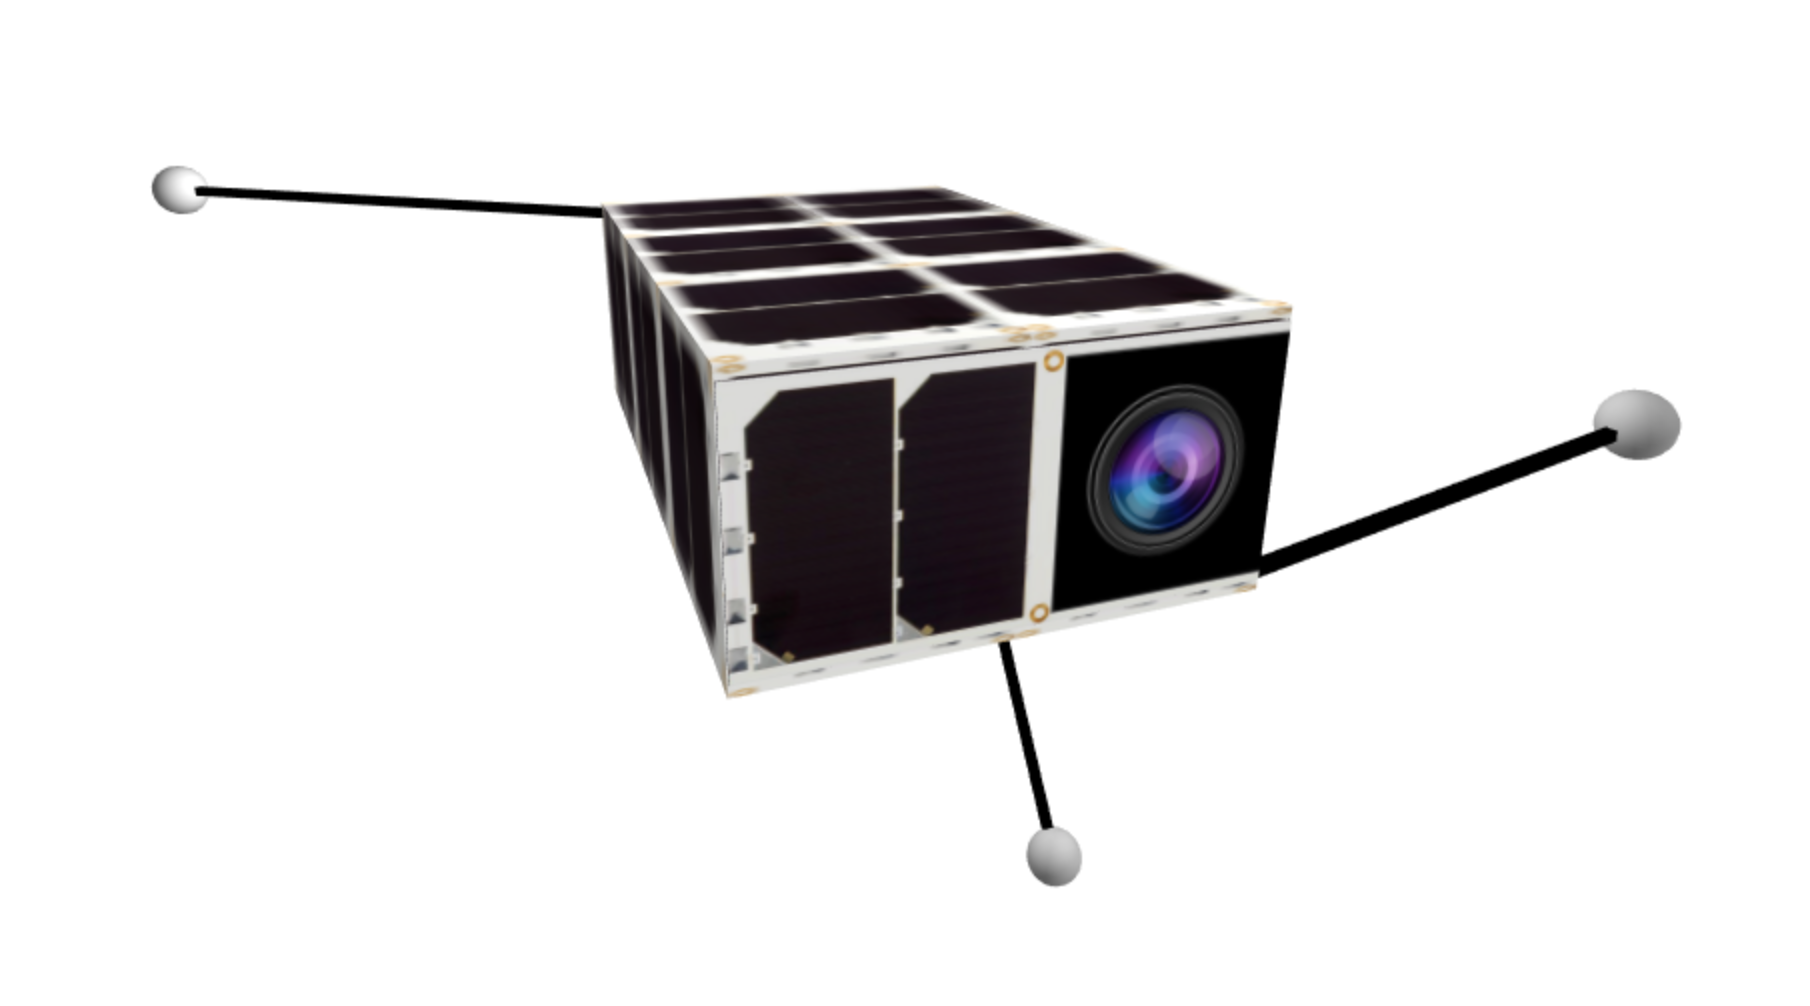
\includegraphics[width=12cm]{Figures/view1.png}
    \caption{Proposed architecture for a 6U CubeSat space telescope. Each boom has a single degree-of-freedom in linearly independent axes, enabling three-axis attitude control. Magnetorquers are used to desaturate the angular momentum of the booms and keep them within their operating limits.}
    \label{fig:meshcat_shot}
\end{figure}

In this paper, a novel actuation strategy for fine-pointing nanosatellites is explored by abandoning high-frequency rotor-based actuators in favor of low-frequency deployable booms, as shown in Figure \ref{fig:meshcat_shot}. By taking advantage of the squared relationship between boom length and the inertia of the boom, tip-mounted masses provide the control authority required for attitude control without having to accelerate or decelerate the booms too aggressively. A nanosatellite would deploy three booms about linearly independent axes and rotate them \textit{slowly} to reject the \textit{slowly} varying disturbance torques. By better matching the actuators' speed to the frequency content of the disturbances, these booms are able to eliminate jitter and enable high-accuracy body pointing of the nanosatellite. By improving body pointing, payloads are no longer restricted to those that can accommodate second-stage correction, and existing payloads can be simplified. 

For nanosatellites in low-Earth orbit, disturbance torques come in the form of drag, solar radiation pressure, magnetic, and gravity-gradient torques. All of these disturbances vary slowly throughout an orbit and can be predicted or estimated with high accuracy.  With knowledge of the incoming disturbance torques, the nanosatellite can formulate a motion plan that accounts for disturbances and keeps the deployable booms from hitting their hard stops by using the onboard magnetorquers to offload angular momentum through interactions with the Earth's magnetic field \cite{gatherer2019,markley2014}. Since nominal operations have the nanosatellites inertially pointing during payload operations, linearized attitude dynamics are sufficiently accurate for planning purposes. This allows for a convex formulation of the motion-planning problem, guaranteeing a globally optimal solution in polynomial time \cite{boyd2004}. 

Our primary contributions in this paper include:
%\vspace{-1em}
\begin{enumerate}
\item The introduction of a novel attitude-actuation strategy for fine-pointing nanosatellites.
\vspace{+2mm}
%\item A frequency analysis of the environmental disturbance torques present on a satellite in low-Earth orbit. \todo{this is from our other paper technically}
\vspace{+2mm}
\item The application of convex optimization to motion planning for nanosatellites with actuated booms.
\vspace{+2mm}
\item An estimator and controller architecture for handling boom control during payload operations.
\end{enumerate}
%\vspace{-1em}

In the remainder of this paper, we first provide details on the simulation environment used for this research in Section~\ref{sec:wigglesat:simenv}. Next, the deployable-boom actuation strategy is discussed in Section \ref{sec:wigglesat:actuation}, and a convex motion planner is developed in Section \ref{sec:wigglesat:planner} to reason about the actuator's constraints.  A lower-level estimation and control architecture is then detailed in Section \ref{sec:wigglesat:control}. Finally, numerical experiments are presented in Section \ref{sec:wigglesat:experiments} to validate the proposed ideas, and results are summarized in Section \ref{sec:wigglesat:conclusion}.

\section{Spacecraft Dynamics Model}
\label{sec:wigglesat:simenv}
This section describes the model used to analyze and simulate the dynamics of a nanosatellite space telescope in low-Earth orbit. Since the spacecraft has no propulsion onboard, the orbital and attitude dynamics are decoupled and can be modeled separately. The open-source Julia package \textit{SatelliteDynamics.jl} is used for orbital simulation, taking into account high order gravity, atmospheric drag, solar radiation pressure, and third-body accelerations. For the attitude dynamics, a rigid-body simulation is used that includes the disturbance torques present in low-Earth orbit. 

We denote the Earth-Centered Inertial frame (ECI) as $\mathbb{E}$, and the spacecraft body frame as $\mathbb{B}$. Relating these two frames is ${}^{\mathbb{B}} Q {}^{\mathbb{E}}$, the rotation matrix that takes vectors expressed in $\mathbb{E}$ and resolves them in frame $\mathbb{B}$.
\subsubsection{Gravity-Gradient Torque}
Gravity varies inversely with the square of the distance from the central body. Because of this, parts of the spacecraft that are farther away from the center of the central body experience a smaller gravitational force than the parts that are closer. The resulting non-uniform gravitational force acting on the spacecraft causes a torque. This torque can be neatly expressed in terms of the spacecraft's attitude, orbital position, and the inertia \cite{markley2014,wertz1978}. First, the normalized position vector is computed in the body frame:
\begin{align}
    \hat{m} &= \frac{{}^{\mathbb{B}} Q {}^{\mathbb{E}} r_{\mathbb{E}}}{\|r_{\mathbb{E}}\|},
\end{align}
then, the gravity-gradient torque can be calculated, 
\begin{align}
    \tau_{gg} &= \frac{3 \mu}{\|r\|^3}(\hat{m} \times J\hat{m}),
\end{align}
where $\mu$ is the standard gravitational parameter for Earth. This calculation only takes into consideration the spherical gravitational term, since the gravity gradient torque from higher-order gravity terms is of negligible magnitude.  For inertially pointing spacecraft in pure Keplerian motion, the resulting gravity gradient torque is periodic with the orbit.

\subsubsection{Atmospheric Drag Torque}
To describe the atmospheric drag torque, the relative velocity of the spacecraft with respect to the atmosphere is calculated with the following:
\begin{align}
    v_{rel} = {}^{\mathbb{B}} Q {}^{\mathbb{E}} ( v_{eci} - \omega_{Earth} \times r_{\mathbb{E}} ).
\end{align}
A normalized version of this vector will be represented as $\hat{v}_{rel} = v_{rel}/\|v_{rel}\|$.
The spacecraft in this experiment has been parameterized as a box with 6 orthogonal faces. This geometry is described with normal vectors $\hat{n}_i$ for each face, position vectors from the center of mass of the spacecraft to the center of pressure of each face $r_i$, and the area of each face $S_i$. Only the faces in the direction of the relative velocity vector are affected, and the force is proportional to the cosine of the angle between the normal face vector and the relative velocity vector. This can also be represented as the dot product between two normalized vectors:
\begin{align}
w_i &= \text{max}(0,v^T [^{\mathbb{E}}Q^{\mathbb{B}} \, \hat{n}_i]).
\end{align}
The force on each face is then calculated with the atmospheric density $\rho$ and the coefficient of drag $C_d$, 
\begin{align}
    F_{aero,i} &= -\frac{1}{2}\rho\, C_d \|v_{rel}\| v_{rel}S_i w_i.
\end{align}
The torque acting on the nanosatelite is then the sum of the moments caused by these forces:
\begin{align}
     \tau_{aero} &=  \sum_{i = 1}^6 r_i \times  F_{aero,i}.
\end{align}
\subsubsection{Solar Radiation Pressure Torque}
Similar to the aerodynamic drag torque, the radiation from the sun carries momentum, and can impart a force on the spacecraft. First, the position vector from the spacecraft to the sun is calculated as:
\begin{align}
    {}^{\mathbb{B}}r{}^{sun} &= {}^{\mathbb{E}}r{}^{sun} - {}^{\mathbb{E}}r{}^{\mathbb{B}},
\end{align}
after which it is expressed in the body frame and normalized:
\begin{align}
     \hat{s} &= \frac{ {}^{\mathbb{B}} Q {}^{\mathbb{E}} \,\,{}^{\mathbb{B}}r{}^{sun}}{\| {}^{\mathbb{B}}r{}^{sun}\|}.
\end{align}
% \begin{align}
%     {}^{B}r{}^{sun} &= {}^{E}r{}^{sun} - {}^{E}r{}^{B} \\ \hat{s} &= \frac{ {}^B Q {}^N, {}^{B}r{}^{sun}}{\| {}^{B}r{}^{sun}\|}.
% \end{align}
Based on the spectral and diffuse reflection coefficients, $R_{spec}$ and $R_{diff}$ respectively, the optical properties of the spacecraft material with respect to solar radiation pressure can be calculated. The combined effects of reflection, diffusion, and absorption are captured in our variable $q_i$, 
\begin{align}
    q_i &=  2\big[ \frac{1}{3}R_{diff} + R_{spec} \hat{s}^T \hat{n}_i\big] \hat{n}_i + (1 - R_{spec})\hat{s}. 
\end{align}
The force caused by radiation pressure on each face is then, 
\begin{align}
    F_{srp,i} &= -P_{sun} S_i q_i \cdot \text{max}(0,\hat{s}^T [^{\mathbb{E}}Q^{\mathbb{B}} \, n_i]),
\end{align}
and the final torque is the sum of the moments caused by the force on each face:
\begin{align}
    \tau_{srp} &=  \sum_{i = 1}^6 r_i \times  F_{srp,i}.
\end{align}
\subsubsection{Magnetic Torques}
We use the International Geomagnetic Reference Field (IGRF) \cite{thebault2015} to model the Earth's magnetic field. The IGRF models the scalar potential of the magnetic field with a spherical harmonic expansion and calculates the magnetic field vector as the negative gradient of this potential with respect to the position.  This potential is described by a set of time-varying coefficients that account for decades of empirical data and can predict the Earth's magnetic field up to 5 years in the future. This resulting magnetic field vector is a function of position and time, and for spacecraft with no propulsion, can be computed online to predict future magnetometer measurements. The spacecraft can then use the onboard magnetorquers to interact with the Earth's magnetic field in the following way:
\begin{align}
    \tau_{mag} = m \times b_{\mathbb{B}},
\end{align}
where $b_{\mathbb{B}}$ is the magnetic field vector expressed in the spacecraft body frame, and $m$ is the spacecraft's magnetic moment in the body frame. The total disturbance torque on the nanosatellite is the sum of the aforementioned torques:
\begin{align}
    \tau = \tau_{gg} + \tau_{aero} + \tau_{srp} + \tau_{mag}.
\end{align}
\section{Actuation Strategy}
\label{sec:wigglesat:actuation}
To justify the introduction of a novel actuation strategy, the nature of the disturbance torques was analyzed.  A 1000-trial Monte-Carlo simulation of the orbital and attitude dynamics was performed and disturbance torques were collected. The orbits in the simulations were at an altitude of 550 km with inclinations between 0$^\circ$ and 90$^\circ$, eccentricities between 0 and 0.00002, and epochs between 2014 and 2017. These dispersions served to capture the full range of potential disturbance torques, as well as accurately sample the time-varying atmospheric density.  A discrete Fourier transform of the disturbance torque data was taken, and the magnitudes of the terms in the Fourier series were used to plot its power-spectral density in Figure \ref{fig:disturbances}. 
\begin{figure}%[H]
    \centering
    % \setlength{\figureheight}{3.0in}
    % \setlength{\figurewidth}{5.0in}
    % % This file was created by matlab2tikz.
%
%The latest updates can be retrieved from
%  http://www.mathworks.com/matlabcentral/fileexchange/22022-matlab2tikz-matlab2tikz
%where you can also make suggestions and rate matlab2tikz.
%
\begin{tikzpicture}

\begin{axis}[%
width=4in,
height=2.0in,
at={(0,0)},
scale only axis,
xmode=log,
xmin=0.0001,
xmax=1000,
xminorticks=true,
xlabel style={font=\color{white!15!black}},
xlabel={Frequency (Hz)},
ymode=log,
ymin=0.01,
ymax=100,
yminorticks=true,
ylabel style={font=\color{white!15!black}},
ylabel={$\text{RMS Torque}\mu N \cdot m/\sqrt{Hz}$},
axis background/.style={fill=white},
axis x line*=bottom,
axis y line*=left,
% legend style={legend cell align=left, align=left, draw=white!15!black}
% ]
legend style={at={(0.5,-0.3)}, anchor=north, legend cell align=left, align=left, draw=white!15!black}
]
\addplot [color=black, forget plot]
  table[row sep=crcr]{%
0	0\\
1e-06	0\\
2e-06	0\\
3e-06	0\\
4e-06	0\\
5e-06	0\\
6e-06	0\\
7e-06	0\\
8e-06	0\\
9e-06	0\\
1e-05	0\\
1.1e-05	0\\
1.2e-05	0\\
1.3e-05	0\\
1.4e-05	0\\
1.5e-05	0\\
1.6e-05	0\\
1.7e-05	0\\
1.8e-05	0\\
1.9e-05	0\\
2e-05	0\\
2.1e-05	0\\
2.2e-05	0\\
2.3e-05	0\\
2.4e-05	0\\
2.5e-05	0\\
2.6e-05	0\\
2.7e-05	0\\
2.8e-05	0\\
2.9e-05	0\\
3e-05	0\\
3.1e-05	0\\
3.2e-05	0\\
3.3e-05	0\\
3.4e-05	0\\
3.5e-05	0\\
3.6e-05	0\\
3.7e-05	0\\
3.8e-05	0\\
3.9e-05	0\\
4e-05	0\\
4.1e-05	0\\
4.2e-05	0\\
4.3e-05	0\\
4.4e-05	0\\
4.5e-05	0\\
4.6e-05	0\\
4.7e-05	0\\
4.8e-05	0\\
4.9e-05	0\\
5e-05	0\\
5.1e-05	0\\
5.2e-05	0\\
5.3e-05	0\\
5.4e-05	0\\
5.5e-05	0\\
5.6e-05	0\\
5.7e-05	0\\
5.8e-05	0\\
5.9e-05	0\\
6e-05	0\\
6.1e-05	0\\
6.2e-05	0\\
6.3e-05	0\\
6.4e-05	0\\
6.5e-05	0\\
6.6e-05	0\\
6.7e-05	0\\
6.8e-05	0\\
6.9e-05	0\\
7e-05	0\\
7.1e-05	0\\
7.2e-05	0\\
7.3e-05	0\\
7.4e-05	0\\
7.5e-05	0\\
7.6e-05	0\\
7.7e-05	0\\
7.8e-05	0\\
7.9e-05	0\\
8e-05	0.247\\
8.1e-05	0.247\\
8.2e-05	0.247\\
8.3e-05	0.248\\
8.4e-05	0.248\\
8.5e-05	0.249\\
8.6e-05	0.249\\
8.7e-05	0.249\\
8.8e-05	0.25\\
8.9e-05	0.251\\
9e-05	0.252\\
9.1e-05	0.253\\
9.2e-05	0.253\\
9.3e-05	0.254\\
9.4e-05	0.255\\
9.5e-05	0.256\\
9.6e-05	0.256\\
9.7e-05	0.257\\
9.8e-05	0.258\\
9.9e-05	0.259\\
0.0001	0.26\\
0.000101	0.26\\
0.000102	0.261\\
0.000103	0.262\\
0.000104	0.263\\
0.000105	0.264\\
0.000106	0.265\\
0.000107	0.266\\
0.000108	0.268\\
0.000109	0.269\\
0.00011	0.27\\
0.000111	0.272\\
0.000112	0.273\\
0.000113	0.274\\
0.000114	0.275\\
0.000115	0.277\\
0.000116	0.278\\
0.000117	0.279\\
0.000118	0.281\\
0.000119	0.282\\
0.00012	0.283\\
0.000121	0.285\\
0.000122	0.286\\
0.000123	0.288\\
0.000124	0.29\\
0.000125	0.293\\
0.000126	0.295\\
0.000127	0.297\\
0.000128	0.3\\
0.000129	0.302\\
0.00013	0.304\\
0.000131	0.307\\
0.000132	0.309\\
0.000133	0.311\\
0.000134	0.313\\
0.000135	0.316\\
0.000136	0.318\\
0.000137	0.32\\
0.000138	0.323\\
0.000139	0.325\\
0.00014	0.329\\
0.000141	0.335\\
0.000142	0.341\\
0.000143	0.347\\
0.000144	0.353\\
0.000145	0.359\\
0.000146	0.365\\
0.000147	0.371\\
0.000148	0.377\\
0.000149	0.383\\
0.00015	0.389\\
0.000151	0.395\\
0.000152	0.401\\
0.000153	0.407\\
0.000154	0.413\\
0.000155	0.419\\
0.000156	0.425\\
0.000157	0.524\\
0.000158	1.25\\
0.000159	1.98\\
0.00016	2.72\\
0.000161	3.45\\
0.000162	4.19\\
0.000163	4.92\\
0.000164	5.65\\
0.000165	6.39\\
0.000166	7.12\\
0.000167	7.86\\
0.000168	8.59\\
0.000169	9.33\\
0.00017	10.1\\
0.000171	10.8\\
0.000172	11.5\\
0.000173	12.3\\
0.000174	13\\
0.000175	12.6\\
0.000176	11.9\\
0.000177	11.2\\
0.000178	10.4\\
0.000179	9.7\\
0.00018	8.97\\
0.000181	8.23\\
0.000182	7.5\\
0.000183	6.77\\
0.000184	6.04\\
0.000185	5.31\\
0.000186	4.57\\
0.000187	3.84\\
0.000188	3.11\\
0.000189	2.38\\
0.00019	1.65\\
0.000191	0.915\\
0.000192	0.424\\
0.000193	0.418\\
0.000194	0.413\\
0.000195	0.408\\
0.000196	0.402\\
0.000197	0.397\\
0.000198	0.392\\
0.000199	0.386\\
0.0002	0.381\\
0.000201	0.376\\
0.000202	0.371\\
0.000203	0.365\\
0.000204	0.36\\
0.000205	0.355\\
0.000206	0.349\\
0.000207	0.344\\
0.000208	0.339\\
0.000209	0.333\\
0.00021	0.333\\
0.000211	0.333\\
0.000212	0.333\\
0.000213	0.333\\
0.000214	0.333\\
0.000215	0.333\\
0.000216	0.333\\
0.000217	0.333\\
0.000218	0.334\\
0.000219	0.334\\
0.00022	0.335\\
0.000221	0.336\\
0.000222	0.337\\
0.000223	0.337\\
0.000224	0.338\\
0.000225	0.339\\
0.000226	0.34\\
0.000227	0.341\\
0.000228	0.343\\
0.000229	0.345\\
0.00023	0.347\\
0.000231	0.349\\
0.000232	0.352\\
0.000233	0.354\\
0.000234	0.356\\
0.000235	0.358\\
0.000236	0.36\\
0.000237	0.362\\
0.000238	0.364\\
0.000239	0.366\\
0.00024	0.369\\
0.000241	0.371\\
0.000242	0.373\\
0.000243	0.375\\
0.000244	0.377\\
0.000245	0.381\\
0.000246	0.384\\
0.000247	0.388\\
0.000248	0.391\\
0.000249	0.395\\
0.00025	0.398\\
0.000251	0.401\\
0.000252	0.405\\
0.000253	0.408\\
0.000254	0.412\\
0.000255	0.415\\
0.000256	0.419\\
0.000257	0.423\\
0.000258	0.427\\
0.000259	0.432\\
0.00026	0.436\\
0.000261	0.441\\
0.000262	0.447\\
0.000263	0.454\\
0.000264	0.46\\
0.000265	0.467\\
0.000266	0.473\\
0.000267	0.48\\
0.000268	0.486\\
0.000269	0.493\\
0.00027	0.5\\
0.000271	0.506\\
0.000272	0.513\\
0.000273	0.519\\
0.000274	0.526\\
0.000275	0.533\\
0.000276	0.539\\
0.000277	0.546\\
0.000278	0.552\\
0.000279	0.56\\
0.00028	0.57\\
0.000281	0.581\\
0.000282	0.592\\
0.000283	0.602\\
0.000284	0.613\\
0.000285	0.624\\
0.000286	0.634\\
0.000287	0.645\\
0.000288	0.656\\
0.000289	0.667\\
0.00029	0.677\\
0.000291	0.688\\
0.000292	0.699\\
0.000293	0.709\\
0.000294	0.72\\
0.000295	0.731\\
0.000296	0.741\\
0.000297	0.76\\
0.000298	0.781\\
0.000299	0.802\\
0.0003	0.823\\
0.000301	0.844\\
0.000302	0.865\\
0.000303	0.886\\
0.000304	0.907\\
0.000305	0.928\\
0.000306	0.949\\
0.000307	0.97\\
0.000308	0.991\\
0.000309	1.01\\
0.00031	1.03\\
0.000311	1.05\\
0.000312	1.07\\
0.000313	1.1\\
0.000314	1.13\\
0.000315	1.19\\
0.000316	1.25\\
0.000317	1.31\\
0.000318	1.37\\
0.000319	1.43\\
0.00032	1.5\\
0.000321	1.56\\
0.000322	1.62\\
0.000323	1.68\\
0.000324	1.74\\
0.000325	1.8\\
0.000326	1.86\\
0.000327	1.92\\
0.000328	1.98\\
0.000329	2.04\\
0.00033	2.1\\
0.000331	2.16\\
0.000332	4.7\\
0.000333	7.41\\
0.000334	10.1\\
0.000335	12.8\\
0.000336	15.6\\
0.000337	18.3\\
0.000338	21\\
0.000339	23.7\\
0.00034	26.4\\
0.000341	29.1\\
0.000342	31.9\\
0.000343	34.6\\
0.000344	37.3\\
0.000345	40\\
0.000346	42.7\\
0.000347	45.4\\
0.000348	48.1\\
0.000349	48.1\\
0.00035	45.4\\
0.000351	42.7\\
0.000352	40\\
0.000353	37.3\\
0.000354	34.6\\
0.000355	31.9\\
0.000356	29.2\\
0.000357	26.5\\
0.000358	23.8\\
0.000359	21.1\\
0.00036	18.4\\
0.000361	15.7\\
0.000362	13\\
0.000363	10.3\\
0.000364	7.57\\
0.000365	4.86\\
0.000366	2.38\\
0.000367	2.31\\
0.000368	2.24\\
0.000369	2.17\\
0.00037	2.1\\
0.000371	2.03\\
0.000372	1.96\\
0.000373	1.89\\
0.000374	1.82\\
0.000375	1.75\\
0.000376	1.68\\
0.000377	1.61\\
0.000378	1.54\\
0.000379	1.47\\
0.00038	1.4\\
0.000381	1.33\\
0.000382	1.26\\
0.000383	1.19\\
0.000384	1.15\\
0.000385	1.13\\
0.000386	1.1\\
0.000387	1.08\\
0.000388	1.06\\
0.000389	1.04\\
0.00039	1.01\\
0.000391	0.99\\
0.000392	0.967\\
0.000393	0.945\\
0.000394	0.922\\
0.000395	0.9\\
0.000396	0.877\\
0.000397	0.855\\
0.000398	0.832\\
0.000399	0.81\\
0.0004	0.787\\
0.000401	0.767\\
0.000402	0.756\\
0.000403	0.745\\
0.000404	0.734\\
0.000405	0.723\\
0.000406	0.712\\
0.000407	0.701\\
0.000408	0.69\\
0.000409	0.679\\
0.00041	0.668\\
0.000411	0.657\\
0.000412	0.646\\
0.000413	0.635\\
0.000414	0.624\\
0.000415	0.613\\
0.000416	0.602\\
0.000417	0.591\\
0.000418	0.58\\
0.000419	0.572\\
0.00042	0.566\\
0.000421	0.559\\
0.000422	0.553\\
0.000423	0.546\\
0.000424	0.54\\
0.000425	0.533\\
0.000426	0.527\\
0.000427	0.52\\
0.000428	0.514\\
0.000429	0.507\\
0.00043	0.501\\
0.000431	0.494\\
0.000432	0.488\\
0.000433	0.481\\
0.000434	0.474\\
0.000435	0.468\\
0.000436	0.462\\
0.000437	0.458\\
0.000438	0.454\\
0.000439	0.45\\
0.00044	0.445\\
0.000441	0.441\\
0.000442	0.437\\
0.000443	0.433\\
0.000444	0.429\\
0.000445	0.424\\
0.000446	0.42\\
0.000447	0.416\\
0.000448	0.412\\
0.000449	0.408\\
0.00045	0.403\\
0.000451	0.399\\
0.000452	0.395\\
0.000453	0.391\\
0.000454	0.388\\
0.000455	0.385\\
0.000456	0.382\\
0.000457	0.379\\
0.000458	0.377\\
0.000459	0.374\\
0.00046	0.371\\
0.000461	0.368\\
0.000462	0.365\\
0.000463	0.363\\
0.000464	0.36\\
0.000465	0.357\\
0.000466	0.354\\
0.000467	0.351\\
0.000468	0.349\\
0.000469	0.346\\
0.00047	0.343\\
0.000471	0.341\\
0.000472	0.339\\
0.000473	0.337\\
0.000474	0.336\\
0.000475	0.334\\
0.000476	0.332\\
0.000477	0.331\\
0.000478	0.329\\
0.000479	0.329\\
0.00048	0.329\\
0.000481	0.328\\
0.000482	0.328\\
0.000483	0.328\\
0.000484	0.328\\
0.000485	0.328\\
0.000486	0.327\\
0.000487	0.327\\
0.000488	0.327\\
0.000489	0.331\\
0.00049	0.334\\
0.000491	0.338\\
0.000492	0.341\\
0.000493	0.344\\
0.000494	0.348\\
0.000495	0.351\\
0.000496	0.355\\
0.000497	0.358\\
0.000498	0.361\\
0.000499	0.365\\
0.0005	0.368\\
0.000501	0.372\\
0.000502	0.375\\
0.000503	0.378\\
0.000504	0.382\\
0.000505	0.385\\
0.000506	0.501\\
0.000507	0.701\\
0.000508	0.902\\
0.000509	1.1\\
0.00051	1.3\\
0.000511	1.5\\
0.000512	1.7\\
0.000513	1.9\\
0.000514	2.1\\
0.000515	2.3\\
0.000516	2.5\\
0.000517	2.7\\
0.000518	2.91\\
0.000519	3.11\\
0.00052	3.31\\
0.000521	3.51\\
0.000522	3.71\\
0.000523	3.8\\
0.000524	3.6\\
0.000525	3.4\\
0.000526	3.2\\
0.000527	2.99\\
0.000528	2.79\\
0.000529	2.59\\
0.00053	2.39\\
0.000531	2.19\\
0.000532	1.99\\
0.000533	1.78\\
0.000534	1.58\\
0.000535	1.38\\
0.000536	1.18\\
0.000537	0.976\\
0.000538	0.774\\
0.000539	0.577\\
0.00054	0.389\\
0.000541	0.353\\
0.000542	0.346\\
0.000543	0.338\\
0.000544	0.332\\
0.000545	0.326\\
0.000546	0.321\\
0.000547	0.315\\
0.000548	0.309\\
0.000549	0.304\\
0.00055	0.298\\
0.000551	0.293\\
0.000552	0.287\\
0.000553	0.281\\
0.000554	0.276\\
0.000555	0.27\\
0.000556	0.264\\
0.000557	0.259\\
0.000558	0.255\\
0.000559	0.253\\
0.00056	0.25\\
0.000561	0.248\\
0.000562	0.246\\
0.000563	0.244\\
0.000564	0.242\\
0.000565	0.24\\
0.000566	0.238\\
0.000567	0.235\\
0.000568	0.233\\
0.000569	0.231\\
0.00057	0.229\\
0.000571	0.227\\
0.000572	0.225\\
0.000573	0.223\\
0.000574	0.22\\
0.000575	0.218\\
0.000576	0.217\\
0.000577	0.216\\
0.000578	0.215\\
0.000579	0.213\\
0.00058	0.212\\
0.000581	0.211\\
0.000582	0.21\\
0.000583	0.208\\
0.000584	0.207\\
0.000585	0.206\\
0.000586	0.205\\
0.000587	0.204\\
0.000588	0.203\\
0.000589	0.202\\
0.00059	0.201\\
0.000591	0.2\\
0.000592	0.198\\
0.000593	0.198\\
0.000594	0.197\\
0.000595	0.196\\
0.000596	0.195\\
0.000597	0.194\\
0.000598	0.194\\
0.000599	0.193\\
0.0006	0.192\\
0.000601	0.191\\
0.000602	0.191\\
0.000603	0.19\\
0.000604	0.189\\
0.000605	0.188\\
0.000606	0.188\\
0.000607	0.187\\
0.000608	0.186\\
0.000609	0.185\\
0.00061	0.185\\
0.000611	0.184\\
0.000612	0.183\\
0.000613	0.183\\
0.000614	0.182\\
0.000615	0.182\\
0.000616	0.181\\
0.000617	0.181\\
0.000618	0.18\\
0.000619	0.18\\
0.00062	0.179\\
0.000621	0.179\\
0.000622	0.178\\
0.000623	0.177\\
0.000624	0.177\\
0.000625	0.176\\
0.000626	0.176\\
0.000627	0.175\\
0.000628	0.175\\
0.000629	0.174\\
0.00063	0.174\\
0.000631	0.174\\
0.000632	0.173\\
0.000633	0.173\\
0.000634	0.173\\
0.000635	0.172\\
0.000636	0.172\\
0.000637	0.172\\
0.000638	0.171\\
0.000639	0.171\\
0.00064	0.171\\
0.000641	0.17\\
0.000642	0.17\\
0.000643	0.17\\
0.000644	0.169\\
0.000645	0.169\\
0.000646	0.169\\
0.000647	0.169\\
0.000648	0.169\\
0.000649	0.169\\
0.00065	0.169\\
0.000651	0.169\\
0.000652	0.169\\
0.000653	0.17\\
0.000654	0.17\\
0.000655	0.17\\
0.000656	0.17\\
0.000657	0.17\\
0.000658	0.17\\
0.000659	0.171\\
0.00066	0.171\\
0.000661	0.171\\
0.000662	0.171\\
0.000663	0.172\\
0.000664	0.174\\
0.000665	0.175\\
0.000666	0.177\\
0.000667	0.178\\
0.000668	0.179\\
0.000669	0.181\\
0.00067	0.182\\
0.000671	0.184\\
0.000672	0.185\\
0.000673	0.187\\
0.000674	0.188\\
0.000675	0.189\\
0.000676	0.191\\
0.000677	0.192\\
0.000678	0.194\\
0.000679	0.195\\
0.00068	0.216\\
0.000681	0.261\\
0.000682	0.307\\
0.000683	0.361\\
0.000684	0.422\\
0.000685	0.482\\
0.000686	0.542\\
0.000687	0.603\\
0.000688	0.667\\
0.000689	0.736\\
0.00069	0.805\\
0.000691	0.875\\
0.000692	0.944\\
0.000693	1.01\\
0.000694	1.08\\
0.000695	1.15\\
0.000696	1.22\\
0.000697	1.29\\
0.000698	1.22\\
0.000699	1.15\\
0.0007	1.08\\
0.000701	1.01\\
0.000702	0.944\\
0.000703	0.875\\
0.000704	0.806\\
0.000705	0.743\\
0.000706	0.685\\
0.000707	0.627\\
0.000708	0.57\\
0.000709	0.512\\
0.00071	0.454\\
0.000711	0.396\\
0.000712	0.339\\
0.000713	0.281\\
0.000714	0.223\\
0.000715	0.198\\
0.000716	0.194\\
0.000717	0.191\\
0.000718	0.188\\
0.000719	0.185\\
0.00072	0.182\\
0.000721	0.178\\
0.000722	0.175\\
0.000723	0.172\\
0.000724	0.169\\
0.000725	0.166\\
0.000726	0.162\\
0.000727	0.159\\
0.000728	0.156\\
0.000729	0.153\\
0.00073	0.15\\
0.000731	0.146\\
0.000732	0.144\\
0.000733	0.143\\
0.000734	0.142\\
0.000735	0.141\\
0.000736	0.14\\
0.000737	0.139\\
0.000738	0.138\\
0.000739	0.138\\
0.00074	0.137\\
0.000741	0.136\\
0.000742	0.135\\
0.000743	0.134\\
0.000744	0.133\\
0.000745	0.132\\
0.000746	0.131\\
0.000747	0.131\\
0.000748	0.13\\
0.000749	0.129\\
0.00075	0.128\\
0.000751	0.128\\
0.000752	0.127\\
0.000753	0.127\\
0.000754	0.126\\
0.000755	0.126\\
0.000756	0.125\\
0.000757	0.125\\
0.000758	0.124\\
0.000759	0.124\\
0.00076	0.123\\
0.000761	0.123\\
0.000762	0.122\\
0.000763	0.122\\
0.000764	0.121\\
0.000765	0.121\\
0.000766	0.12\\
0.000767	0.12\\
0.000768	0.12\\
0.000769	0.119\\
0.00077	0.119\\
0.000771	0.119\\
0.000772	0.119\\
0.000773	0.118\\
0.000774	0.118\\
0.000775	0.118\\
0.000776	0.117\\
0.000777	0.117\\
0.000778	0.117\\
0.000779	0.116\\
0.00078	0.116\\
0.000781	0.116\\
0.000782	0.116\\
0.000783	0.115\\
0.000784	0.115\\
0.000785	0.115\\
0.000786	0.115\\
0.000787	0.114\\
0.000788	0.114\\
0.000789	0.114\\
0.00079	0.114\\
0.000791	0.113\\
0.000792	0.113\\
0.000793	0.113\\
0.000794	0.113\\
0.000795	0.113\\
0.000796	0.112\\
0.000797	0.112\\
0.000798	0.112\\
0.000799	0.112\\
0.0008	0.112\\
0.000801	0.111\\
0.000802	0.111\\
0.000803	0.111\\
0.000804	0.111\\
0.000805	0.111\\
0.000806	0.111\\
0.000807	0.112\\
0.000808	0.112\\
0.000809	0.112\\
0.00081	0.112\\
0.000811	0.113\\
0.000812	0.113\\
0.000813	0.113\\
0.000814	0.113\\
0.000815	0.113\\
0.000816	0.114\\
0.000817	0.114\\
0.000818	0.114\\
0.000819	0.114\\
0.00082	0.115\\
0.000821	0.115\\
0.000822	0.116\\
0.000823	0.116\\
0.000824	0.117\\
0.000825	0.118\\
0.000826	0.118\\
0.000827	0.119\\
0.000828	0.119\\
0.000829	0.12\\
0.00083	0.12\\
0.000831	0.121\\
0.000832	0.121\\
0.000833	0.122\\
0.000834	0.123\\
0.000835	0.123\\
0.000836	0.124\\
0.000837	0.125\\
0.000838	0.127\\
0.000839	0.129\\
0.00084	0.131\\
0.000841	0.133\\
0.000842	0.135\\
0.000843	0.137\\
0.000844	0.139\\
0.000845	0.141\\
0.000846	0.143\\
0.000847	0.145\\
0.000848	0.147\\
0.000849	0.149\\
0.00085	0.151\\
0.000851	0.153\\
0.000852	0.155\\
0.000853	0.157\\
0.000854	0.166\\
0.000855	0.203\\
0.000856	0.253\\
0.000857	0.307\\
0.000858	0.361\\
0.000859	0.415\\
0.00086	0.469\\
0.000861	0.523\\
0.000862	0.576\\
0.000863	0.63\\
0.000864	0.684\\
0.000865	0.738\\
0.000866	0.792\\
0.000867	0.846\\
0.000868	0.9\\
0.000869	0.954\\
0.00087	1.01\\
0.000871	1.06\\
0.000872	1.04\\
0.000873	0.985\\
0.000874	0.934\\
0.000875	0.884\\
0.000876	0.833\\
0.000877	0.782\\
0.000878	0.731\\
0.000879	0.681\\
0.00088	0.63\\
0.000881	0.579\\
0.000882	0.528\\
0.000883	0.478\\
0.000884	0.427\\
0.000885	0.376\\
0.000886	0.325\\
0.000887	0.275\\
0.000888	0.224\\
0.000889	0.189\\
0.00089	0.184\\
0.000891	0.179\\
0.000892	0.174\\
0.000893	0.17\\
0.000894	0.165\\
0.000895	0.16\\
0.000896	0.155\\
0.000897	0.15\\
0.000898	0.145\\
0.000899	0.14\\
0.0009	0.135\\
0.000901	0.131\\
0.000902	0.126\\
0.000903	0.121\\
0.000904	0.116\\
0.000905	0.111\\
0.000906	0.106\\
0.000907	0.105\\
0.000908	0.103\\
0.000909	0.102\\
0.00091	0.101\\
0.000911	0.1\\
0.000912	0.099\\
0.000913	0.0979\\
0.000914	0.0968\\
0.000915	0.0957\\
0.000916	0.0946\\
0.000917	0.0936\\
0.000918	0.0925\\
0.000919	0.0916\\
0.00092	0.0909\\
0.000921	0.0902\\
0.000922	0.0895\\
0.000923	0.0887\\
0.000924	0.0883\\
0.000925	0.0881\\
0.000926	0.0878\\
0.000927	0.0876\\
0.000928	0.0873\\
0.000929	0.087\\
0.00093	0.0868\\
0.000931	0.0865\\
0.000932	0.0862\\
0.000933	0.086\\
0.000934	0.0857\\
0.000935	0.0855\\
0.000936	0.0852\\
0.000937	0.0849\\
0.000938	0.0847\\
0.000939	0.0844\\
0.00094	0.0841\\
0.000941	0.0839\\
0.000942	0.0837\\
0.000943	0.0835\\
0.000944	0.0833\\
0.000945	0.0832\\
0.000946	0.083\\
0.000947	0.0828\\
0.000948	0.0826\\
0.000949	0.0824\\
0.00095	0.0823\\
0.000951	0.0821\\
0.000952	0.0819\\
0.000953	0.0817\\
0.000954	0.0815\\
0.000955	0.0814\\
0.000956	0.0812\\
0.000957	0.081\\
0.000958	0.0808\\
0.000959	0.0807\\
0.00096	0.0805\\
0.000961	0.0804\\
0.000962	0.0803\\
0.000963	0.0802\\
0.000964	0.0801\\
0.000965	0.0799\\
0.000966	0.0798\\
0.000967	0.0797\\
0.000968	0.0796\\
0.000969	0.0795\\
0.00097	0.0793\\
0.000971	0.0792\\
0.000972	0.0791\\
0.000973	0.079\\
0.000974	0.0789\\
0.000975	0.0787\\
0.000976	0.0786\\
0.000977	0.0786\\
0.000978	0.0785\\
0.000979	0.0785\\
0.00098	0.0784\\
0.000981	0.0783\\
0.000982	0.0783\\
0.000983	0.0782\\
0.000984	0.0782\\
0.000985	0.0781\\
0.000986	0.078\\
0.000987	0.078\\
0.000988	0.0779\\
0.000989	0.0779\\
0.00099	0.0778\\
0.000991	0.0777\\
0.000992	0.0777\\
0.000993	0.0776\\
0.000994	0.0776\\
0.000995	0.0776\\
0.000996	0.0776\\
0.000997	0.0776\\
0.000998	0.0776\\
0.000999	0.0776\\
0.001	0.0776\\
0.00105	0.477\\
0.0011	0.0628\\
0.00115	0.0596\\
0.0012	0.0862\\
0.00125	0.0736\\
0.0013	0.0558\\
0.00135	0.0531\\
0.0014	0.157\\
0.00145	0.0478\\
0.0015	0.0452\\
0.00155	0.0618\\
0.0016	0.0675\\
0.00165	0.0429\\
0.0017	0.0411\\
0.00175	0.117\\
0.0018	0.041\\
0.00185	0.0407\\
0.0019	0.0552\\
0.00195	0.0428\\
0.002	0.0325\\
0.00205	0.0323\\
0.0021	0.0906\\
0.00215	0.0351\\
0.0022	0.0294\\
0.00225	0.0439\\
0.0023	0.0429\\
0.00235	0.0354\\
0.0024	0.0332\\
0.00245	0.0534\\
0.0025	0.0297\\
0.00255	0.0303\\
0.0026	0.0457\\
0.00265	0.031\\
0.0027	0.0268\\
0.00275	0.0252\\
0.0028	0.0316\\
0.00285	0.0259\\
0.0029	0.0255\\
0.00295	0.038\\
0.003	0.0301\\
0.00305	0.0213\\
0.0031	0.0218\\
0.00315	0.048\\
0.0032	0.0251\\
0.00325	0.0224\\
0.0033	0.0325\\
0.00335	0.0215\\
0.0034	0.0208\\
0.00345	0.0229\\
0.0035	0.05\\
0.00355	0.0186\\
0.0036	0.0188\\
0.00365	0.0311\\
0.0037	0.0205\\
0.00375	0.0193\\
0.0038	0.0199\\
0.00385	0.0326\\
0.0039	0.0174\\
0.00395	0.0178\\
0.004	0.0349\\
0.00405	0.0204\\
0.0041	0.0175\\
0.00415	0.0176\\
0.0042	0.0211\\
0.00425	0.0164\\
0.0043	0.0163\\
0.00435	0.0299\\
0.0044	0.0182\\
0.00445	0.0156\\
0.0045	0.0176\\
0.00455	0.0339\\
0.0046	0.0157\\
0.00465	0.0146\\
0.0047	0.028\\
0.00475	0.0153\\
0.0048	0.0148\\
0.00485	0.0153\\
0.0049	0.037\\
0.00495	0.0138\\
0.005	0.0135\\
0.00505	0.0323\\
0.0051	0.0142\\
0.00515	0.0137\\
0.0052	0.0138\\
0.00525	0.0219\\
0.0053	0.0129\\
0.00535	0.013\\
0.0054	0.0314\\
0.00545	0.0136\\
0.0055	0.0123\\
0.00555	0.0124\\
0.0056	0.0164\\
0.00565	0.0127\\
0.0057	0.0128\\
0.00575	0.0358\\
0.0058	0.0123\\
0.00585	0.0118\\
0.0059	0.0132\\
0.00595	0.0267\\
0.006	0.0113\\
0.00605	0.0115\\
0.0061	0.0282\\
0.00615	0.0128\\
0.0062	0.0114\\
0.00625	0.0125\\
0.0063	0.0208\\
0.00635	0.0102\\
0.0064	0.0104\\
0.00645	0.0228\\
0.0065	0.0103\\
0.00655	0.0104\\
0.0066	0.011\\
0.00665	0.0148\\
0.0067	0.0101\\
0.00675	0.0106\\
0.0068	0.0219\\
0.00685	0.00994\\
0.0069	0.00937\\
0.00695	0.0105\\
0.007	0.0103\\
0.00705	0.00965\\
0.0071	0.00996\\
0.00715	0.019\\
0.0072	0.00945\\
0.00725	0.00926\\
0.0073	0.0124\\
0.00735	0.011\\
0.0074	0.0086\\
0.00745	0.00882\\
0.0075	0.016\\
0.00755	0.0088\\
0.0076	0.00902\\
0.00765	0.00989\\
0.0077	0.0114\\
0.00775	0.00828\\
0.0078	0.00863\\
0.00785	0.0154\\
0.0079	0.00868\\
0.00795	0.00889\\
0.008	0.0087\\
0.00805	0.00938\\
0.0081	0.00834\\
0.00815	0.00867\\
0.0082	0.0198\\
0.00825	0.00758\\
0.0083	0.00781\\
0.00835	0.00974\\
0.0084	0.00761\\
0.00845	0.00768\\
0.0085	0.00792\\
0.00855	0.0167\\
0.0086	0.00789\\
0.00865	0.00762\\
0.0087	0.00984\\
0.00875	0.0111\\
0.0088	0.0073\\
0.00885	0.0074\\
0.0089	0.0149\\
0.00895	0.00718\\
0.009	0.00726\\
0.00905	0.00963\\
0.0091	0.0132\\
0.00915	0.00694\\
0.0092	0.00706\\
0.00925	0.0168\\
0.0093	0.00895\\
0.00935	0.00851\\
0.0094	0.00779\\
0.00945	0.00817\\
0.0095	0.0079\\
0.00955	0.00868\\
0.0096	0.0193\\
0.00965	0.00715\\
0.0097	0.00697\\
0.00975	0.0113\\
0.0098	0.00688\\
0.00985	0.00664\\
0.0099	0.00688\\
0.00995	0.017\\
0.01	0.00629\\
0.01005	0.00651\\
0.0101	0.0105\\
0.01015	0.0129\\
0.0102	0.00707\\
0.01025	0.00621\\
0.0103	0.0149\\
0.01035	0.00785\\
0.0104	0.00669\\
0.01045	0.0126\\
0.0105	0.0105\\
0.01055	0.0062\\
0.0106	0.00662\\
0.01065	0.0131\\
0.0107	0.0069\\
0.01075	0.00677\\
0.0108	0.0133\\
0.01085	0.00716\\
0.0109	0.00661\\
0.01095	0.00769\\
0.011	0.0133\\
0.01105	0.00657\\
0.0111	0.00626\\
0.01115	0.0144\\
0.0112	0.00609\\
0.01125	0.00587\\
0.0113	0.00581\\
0.01135	0.00995\\
0.0114	0.00594\\
0.01145	0.00611\\
0.0115	0.0111\\
0.01155	0.0095\\
0.0116	0.00583\\
0.01165	0.00597\\
0.0117	0.00933\\
0.01175	0.00711\\
0.0118	0.00578\\
0.01185	0.0114\\
0.0119	0.00665\\
0.01195	0.00545\\
0.012	0.006\\
0.01205	0.00936\\
0.0121	0.00543\\
0.01215	0.00534\\
0.0122	0.00898\\
0.01225	0.00582\\
0.0123	0.00551\\
0.01235	0.00554\\
0.0124	0.0111\\
0.01245	0.00579\\
0.0125	0.00543\\
0.01255	0.00813\\
0.0126	0.0055\\
0.01265	0.00534\\
0.0127	0.00574\\
0.01275	0.00939\\
0.0128	0.00549\\
0.01285	0.00548\\
0.0129	0.00819\\
0.01295	0.00571\\
0.013	0.00503\\
0.01305	0.00535\\
0.0131	0.00794\\
0.01315	0.00526\\
0.0132	0.00525\\
0.01325	0.00701\\
0.0133	0.00498\\
0.01335	0.00501\\
0.0134	0.00516\\
0.01345	0.0108\\
0.0135	0.00487\\
0.01355	0.0053\\
0.0136	0.00746\\
0.01365	0.00513\\
0.0137	0.0051\\
0.01375	0.00533\\
0.0138	0.0139\\
0.01385	0.00474\\
0.0139	0.00478\\
0.01395	0.00649\\
0.014	0.00502\\
0.01405	0.0048\\
0.0141	0.00486\\
0.01415	0.00907\\
0.0142	0.00482\\
0.01425	0.00496\\
0.0143	0.00935\\
0.01435	0.00491\\
0.0144	0.00469\\
0.01445	0.00586\\
0.0145	0.00707\\
0.01455	0.00468\\
0.0146	0.00475\\
0.01465	0.00739\\
0.0147	0.00564\\
0.01475	0.00461\\
0.0148	0.0056\\
0.01485	0.00864\\
0.0149	0.0046\\
0.01495	0.0054\\
0.015	0.00772\\
0.01505	0.0045\\
0.0151	0.00475\\
0.01515	0.0062\\
0.0152	0.00873\\
0.01525	0.00428\\
0.0153	0.00447\\
0.01535	0.00744\\
0.0154	0.00428\\
0.01545	0.00425\\
0.0155	0.00447\\
0.01555	0.00645\\
0.0156	0.00432\\
0.01565	0.00448\\
0.0157	0.00822\\
0.01575	0.00456\\
0.0158	0.00413\\
0.01585	0.005\\
0.0159	0.00429\\
0.01595	0.00409\\
0.016	0.00422\\
0.01605	0.00618\\
0.0161	0.00458\\
0.01615	0.00416\\
0.0162	0.00465\\
0.01625	0.00521\\
0.0163	0.00429\\
0.01635	0.00403\\
0.0164	0.00586\\
0.01645	0.00392\\
0.0165	0.00455\\
0.01655	0.00556\\
0.0166	0.00454\\
0.01665	0.00386\\
0.0167	0.00411\\
0.01675	0.00631\\
0.0168	0.00371\\
0.01685	0.00384\\
0.0169	0.00403\\
0.01695	0.00451\\
0.017	0.00384\\
0.01705	0.00399\\
0.0171	0.00634\\
0.01715	0.00443\\
0.0172	0.00374\\
0.01725	0.00387\\
0.0173	0.00422\\
0.01735	0.004\\
0.0174	0.00381\\
0.01745	0.00444\\
0.0175	0.00364\\
0.01755	0.00375\\
0.0176	0.00409\\
0.01765	0.00476\\
0.0177	0.0036\\
0.01775	0.00362\\
0.0178	0.0042\\
0.01785	0.00359\\
0.0179	0.00376\\
0.01795	0.00395\\
0.018	0.00408\\
0.01805	0.00358\\
0.0181	0.00398\\
0.01815	0.00444\\
0.0182	0.00347\\
0.01825	0.00348\\
0.0183	0.00348\\
0.01835	0.00412\\
0.0184	0.00354\\
0.01845	0.00361\\
0.0185	0.00449\\
0.01855	0.00342\\
0.0186	0.00345\\
0.01865	0.00368\\
0.0187	0.00372\\
0.01875	0.00344\\
0.0188	0.00341\\
0.01885	0.00375\\
0.0189	0.00343\\
0.01895	0.00346\\
0.019	0.00374\\
0.01905	0.00361\\
0.0191	0.00332\\
0.01915	0.00335\\
0.0192	0.0034\\
0.01925	0.00333\\
0.0193	0.00334\\
0.01935	0.00338\\
0.0194	0.00366\\
0.01945	0.00334\\
0.0195	0.00338\\
0.01955	0.00373\\
0.0196	0.00333\\
0.01965	0.00328\\
0.0197	0.0033\\
0.01975	0.00333\\
0.0198	0.00328\\
0.01985	0.00328\\
0.0199	0.00377\\
0.01995	0.00323\\
};
% \addlegendentry{Maximum RMS}
% \addlegendentry{}

\addplot[area legend, draw=black, fill=blue, draw opacity=0, fill opacity=0.3]
table[row sep=crcr] {%
x	y\\
10	0.0001\\
1000	0.0001\\
1000	100000000\\
10	100000000\\
}--cycle;
\addlegendentry{Reaction Wheel Control/Jitter}

\addplot[area legend, pattern = crosshatch, pattern color = black]
table[row sep=crcr] {%
x	y\\
100	0.0001\\
1000	0.0001\\
1000	100000000\\
100	100000000\\
}--cycle;
\addlegendentry{Structural Modes}

\end{axis}
\end{tikzpicture}%
% % This file was created by matlab2tikz.

    \includegraphics[width=6in]{Figures/mc_frequencies_2.tikz}
    \caption{The frequency content of disturbance torques on a small satellite in low-Earth orbit. Disturbances are due to atmospheric drag, solar radiation pressure, and the gravity gradient. The frequency content of the disturbances is of significantly lower frequency than both standard reaction wheels and structural modes of the nanosatellites.}
    \label{fig:disturbances}
    % \vspace{-10pt}
\end{figure}

Figure \ref{fig:disturbances} displays a clear mismatch between the speed of the disturbances and the speed of the actuators currently used in space telescopes. Jitter from traditional reaction wheels and the structural modes of the spacecraft is 3-4 orders of magnitude faster than the disturbance torques. This mismatch strongly suggests that slower actuators could be used, and as a result, interactions between the actuators and structural modes could be avoided. 

The proposed architecture is displayed in Figure \ref{fig:meshcat_shot}, with three masses mounted to deployable booms that will be used for full three-axis attitude control. Each deployable boom has a single-degree-of-freedom actuator at the interface between the boom and the spacecraft that can rotate the boom and mass combination. By moving the booms, angular momentum is transferred from the body of the spacecraft to the masses, allowing for full actuation of the spacecraft's attitude.  This actuation strategy is significantly slower than reaction wheels, and will therefore avoid both high-frequency jitter as well as the excitement of the flexible modes of the spacecraft. 

Two potential boom-actuator configurations are described in Figures \ref{fig:stepper} and \ref{fig:voice}, with a stepper motor and a linear voice coil respectively. Both of these actuators are able to precisely move the boom, but will also impart constraints on the torque, velocity, and configurations of the boom. These constraints will be accounted for by the onboard motion planner to ensure full attitude actuation is maintained. The boom actuators themselves can also contribute unwanted dynamics, like cogging torques and stiction, into the dynamics of the boom. Care must be taken when designing and building these actuators to ensure that these contributions to the dynamics are well characterized and incorporated into the planner. 
\begin{figure}
    \centering
    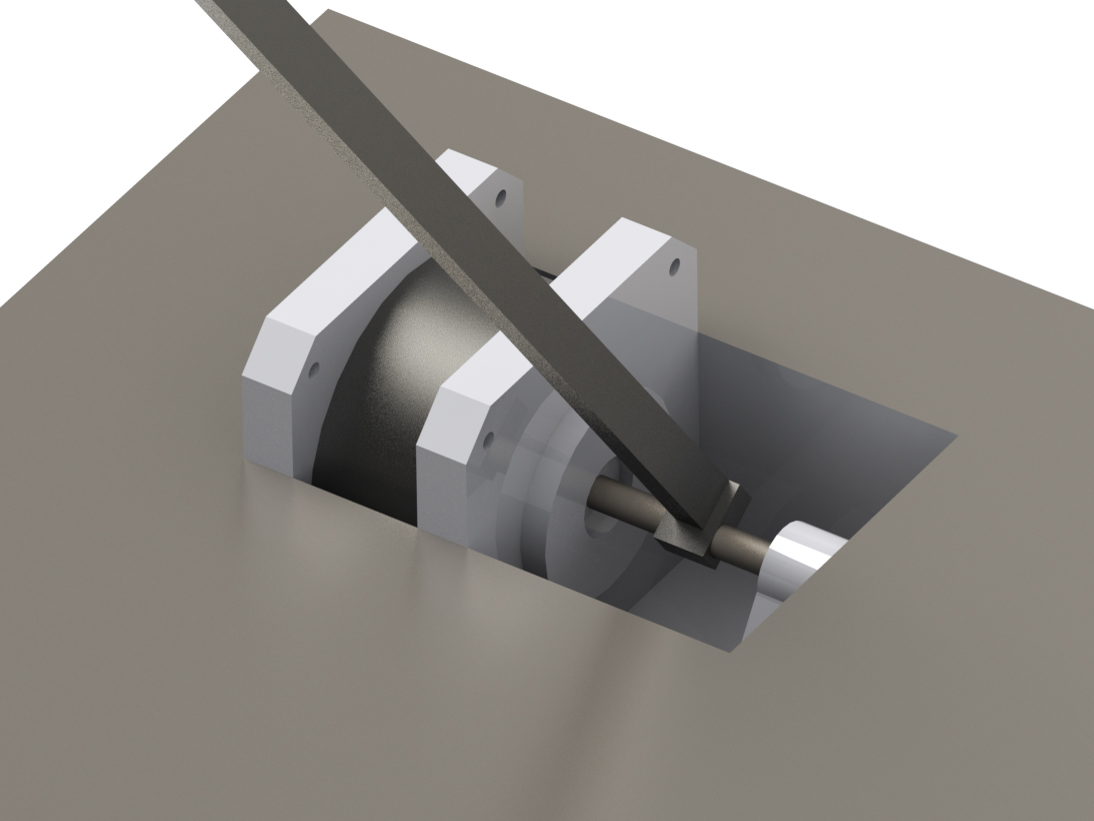
\includegraphics[width=.5\linewidth]{Figures/stepper_render.jpg}
    \caption{Boom actuation with a direct-drive micro-stepper motor. Torques commanded by the micro-stepper will accelerate and decelerate the boom, fully controlling the attitude of the nanosatellite.}
    \label{fig:stepper}
\end{figure}
\begin{figure}
    \centering
    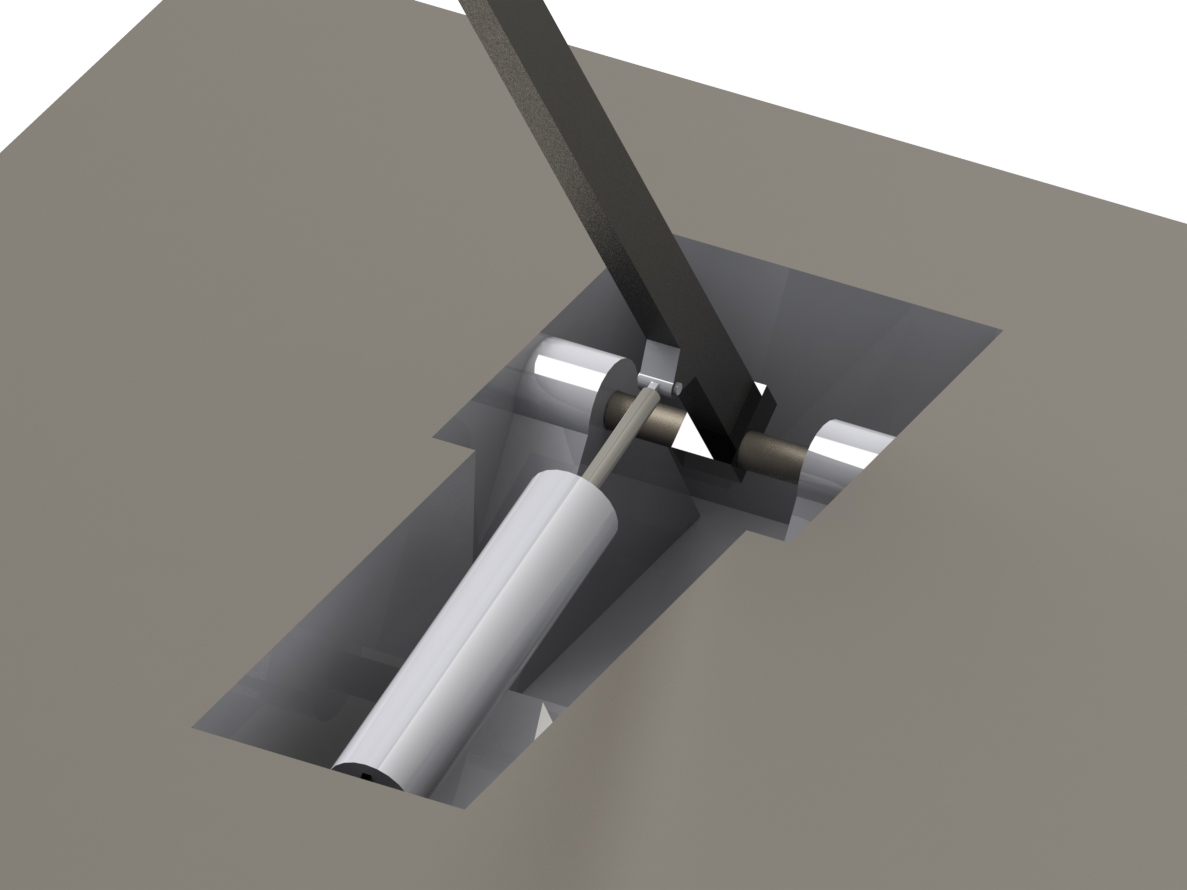
\includegraphics[width=.5\linewidth]{Figures/voice_coil_render.jpg}
    \caption{Boom actuation with a linear voice-coil actuator. By extending and contracting, the linear force is converted to a torque near the base of the boom. This moment in turn controls the angular acceleration of the boom.}
    \label{fig:voice}
\end{figure}
\section{Motion Planner}
\label{sec:wigglesat:planner}
The spacecraft must maintain pointing through a balance of magnetorquer control and boom control. A holistic planning approach is taken due to the following constraints: The magnetorquers cannot be used during payload operations, and the deployable booms must stay within their allowable ranges in position, velocity, and acceleration.  Coarse attitude control has been demonstrated using only magnetorquers \cite{gatherer2019}, but this control strategy is not precise enough for ultra-fine pointing and relies on a varying magnetic field to demonstrate full three-axis actuation. The booms provide full three-degree-of-freedom actuation of the attitude but must avoid violating their actuator constraints. These conditions can be combined into a motion planner that balances magnetorquer use for coarse pointing and momentum desaturation while utilizing the booms for precise pointing during periods of payload operation. Similar to the existing nanosatellite telescopes DeMi \cite{allan2018} and ASTERIA \cite{knapp2020}, this motion planner is tailored to the case where exposures are to be taken during eclipse. This means that the nanosatellite must turn off the magnetorquers for the duration of the $\sim$ 35-minute exposures.  

The angular positions of the booms are described with $\theta \in {\mathbb{R}}^3$, and the angular velocities of the booms as $\dot{\theta} \in {\mathbb{R}}^3$. The control input responsible for boom actuation is the angular acceleration of the booms, denoted as $\alpha \in {\mathbb{R}}^3$.  The dynamics of the booms themselves are modeled as double integrators with angular acceleration as a control input:
\begin{align}
	\ddot{\theta} &= \alpha.
\end{align}
Assuming a zero-order hold on the commanded angular acceleration and discretizing, we have,
\begin{align}
    \begin{bmatrix}\theta_{k+1}\\ \dot{\theta}_{k+1} \end{bmatrix} &= A \begin{bmatrix}\theta_{k} \\ \dot{\theta}_{k} \end{bmatrix}  +  B \alpha_k,
\end{align}
where $A$ and $B$ are a function of the sample time, $dt$:
\begin{align}
    A &= \begin{bmatrix} I_3 & dt\cdot I_3 \\ 0_3 & I_3 \end{bmatrix}, \\ 
    B &= \begin{bmatrix} \frac{1}{2} dt^2 \cdot  I_3 \\ dt \cdot I_3 \end{bmatrix}.
\end{align}
The planning problem is then posed as a convex optimization problem where the optimal sequence of actuator commands, magnetic moment $m$ and boom angular acceleration $\alpha$, are solved for that counter all expected disturbance torques. To ensure that the magnetorquers are never on during payload operations, the optimization formulation conservatively prohibits any magnetorquer usage during periods of eclipse, denoted as indexes $k \in \mathcal{E}$. The full optimization problem can be written as follows: 
\begin{mini}
  {m,\alpha, \theta, \dot{\theta}}{\sum_{k=1}^{N} \|[m_k^T,\,\,\gamma \alpha_k^T,\,\,\beta \theta_k^T,\,\,\sigma \dot{\theta}_k^T]^T\|^2}
  {\label{QP}}
  {}
  \addConstraint{\tau_k=}{ m_k \times b_{\mathbb{B}} -J_{boom}\alpha_k}{\forall k} 
  \addConstraint{\begin{bmatrix}\theta_{k+1}\\ \dot{\theta}_{k+1} \end{bmatrix}=}{ A \begin{bmatrix}\theta_{k} \\ \dot{\theta}_{k} \end{bmatrix}  +  B \alpha_k}{\forall k}
  \addConstraint{m_{min} \leq}{m_k \leq m_{max}}{\forall k}
  \addConstraint{\alpha_{min} \leq}{\alpha_k \leq \alpha_{max}}{\forall k}
  \addConstraint{\theta_{min} \leq}{\theta_k \leq \theta_{max}}{\forall k}
  \addConstraint{\dot{\theta}_{min} \leq}{\dot{\theta}_k \leq \dot{\theta}_{max}}{\forall k}
  \addConstraint{m_k=}{0}{\forall k \in \mathcal{E},}
\end{mini}
where the inertias of the deployable booms are the diagonal entries of $J_{boom}$, the magnetic field of the Earth expressed in the spacecraft body frame is $b_{\mathbb{B}}$, and the disturbance torque is $\tau$. The torque matching constraint and the kinematics of the boom are both enforced as linear equality constraints, and all the state and actuator limits are expressed as box inequality constraints \cite{stellato}. The cost function is a quadratic penalty on control usage for the two sets of actuators, with $\gamma$, $\beta$, and $\sigma$ as tuning parameters. Since the cost function is quadratic and positive definite and the constraints are all linear, problem \ref{QP} can be expressed as a convex Quadratic Program (QP).  There are many readily available and robust QP solvers available that are able to find the global optimum, as well as many specialized solvers for use on embedded systems \cite{mattingley2012,stellato,banjac2017}.  Using one of these tools, a highly performant customized solver can be generated for this specific problem, and can be implemented on compute-constrained flight hardware.
\begin{figure*}
\centering
\includegraphics[width=5in]{Figures/jump_solution.tikz}
\caption{Motion plan for a nanosatellite with control over both boom torques and magnetorquers, given estimated future disturbance torques. During eclipse, when payload operations take place, the nanosatellite is constrained to only use the boom torques due to their precision.}
\label{fig:jumpsolution}
\end{figure*}
\section{Estimation and Control}
\label{sec:wigglesat:control}
Fine-pointing nanosatellites demand the strictest pointing requirements during periods of payload operation. The boom actuators are solely responsible for attitude control during these periods since the magnetorquers are too coarse. The planner is able to leverage predicted disturbance torques to put the booms in a configuration that allows for full controllability during the exposure, but these predicted disturbance torques are not accurate enough to feed forward to the controller during these sensitive payload operations. Instead, during image captures, these disturbance torques will be estimated online in a recursive filter, and the online estimate of the disturbance torque will be incorporated as a feedforward control input. This section details the state estimator and controller combination that is used to maintain high-accuracy pointing during periods of image capture.
\subsection{State Estimator}
The disturbance torques on the nanosatellite are smooth and slowly varying, as shown in Figure \ref{fig:torque}. A Multiplicative Extended Kalman Filter (MEKF) will be used for simultaneous estimation of the attitude, angular velocity, and disturbance torque \cite{markley2014}. Conventional MEKF's on large spacecraft omit the spacecraft's angular velocity from the state due to the accuracy of the onboard gyroscope. Nanosatellites do not have gyroscopes of this caliber and must estimate the angular velocity online as a result. The filter state is denoted $z$, and is augmented to include both the disturbance torque $\hat{\tau}$, as well as its first derivative:
\begin{align}
    z &= \begin{bmatrix} q ^T & \omega^T & \hat \tau^T & \dot{\hat \tau}^T\end{bmatrix}^T,
\end{align}
where $q \in {\mathbb{R}}^4$ is the quaternion describing the rotation from $\mathbb{E}$ to the body frame $\mathbb{B}$, $\omega \in {\mathbb{R}}^3$ is the angular velocity of the nanosatellite, $ \hat \tau \in {\mathbb{R}}^3$ is the disturbance torque, and $\dot{\hat \tau} \in {\mathbb{R}}^3$ is its time derivative. Estimating the disturbance torque derivative allows the filter to better predict and anticipate changes in the disturbance torque. The deterministic dynamics model for the MEKF is as follows:
\begin{align}
\dot{z} &=  \begin{bmatrix} \frac{1}{2} q \otimes (\omega) \\ J^{-1}(\hat \tau  - J_{boom}\alpha - \omega \times J\omega )\\ \dot{ \hat{\tau}} \\ 0
\end{bmatrix}.
\end{align}
These dynamics are discretized using an explicit integrator for a given sample time $\Delta t$, and additive white Gaussian (AWGN) process noise, $\nu_x$, is added as follows:
\begin{align}
    z_{k+1} &= f(z_{k},\alpha_k,\Delta t) + \nu_{x}.
\end{align}
In the measurement model, we assume full measurements of the attitude and angular velocity,
\begin{align}
y &= \begin{bmatrix}q \\ \omega \end{bmatrix} + \nu_y,
\end{align}
where $\nu_y$ is AWGN sensor noise. From here, the MEKF as described in \cite{markley2014} is implemented with the addition of the angular velocity to the estimator state. 

\subsection{Feedback Controller}
By linearizing the dynamics of the nanosatellite about a nominal desired attitude, and replacing the quaternion with an axis-angle vector $\phi\in {\mathbb{R}}^3$, the local error dynamics can be expressed as the following:
% \begin{align}
% \dot{x}_{lqr} = \begin{bmatrix} \dot{\phi} \\ \dot{\omega} \\ \dot{\tau} \\ \ddot{\tau}\end{bmatrix} &= \begin{bmatrix} 0_3 & I_3 & 0_3 & 0_3 \\ 0_3 & 0_3 & J^{-1} & 0_3 \\ 0_3 & 0_3 & 0_3 & I_3 \\ 0_3 & 0_3 & 0_3 & 0_3
% \end{bmatrix}\begin{bmatrix} {\phi} \\ {\omega} \\ {\tau} \\ \dot{\tau}\end{bmatrix} + \begin{bmatrix}0_3 \\ -J_{boom} \\ 0_3 \\ 0_3 \end{bmatrix} \alpha 
% \end{align}
\begin{align}
\dot{x}_{lqr} = \begin{bmatrix} \dot{\phi} \\ \dot{\omega}\end{bmatrix} &= \begin{bmatrix} 0 & I  \\ 0 & 0 
\end{bmatrix}\begin{bmatrix} {\phi} \\ {\omega} \end{bmatrix} + \begin{bmatrix}0 \\ -J_{boom} \end{bmatrix} \alpha .
\end{align}
From here, the dynamics can be discretized assuming a zero-order hold on $\alpha$, and a feedback gain $K$ is solved for that minimizes the following infinite-horizon Linear Quadratic Regulator (LQR) cost function:
\begin{align}
\ell(x,u) = \frac{1}{2}\sum_{k=0}^\infty x_{k}^TQx_{k} + \alpha_k^TR\alpha_k , 
\end{align}
where $Q\in {\mathbb{R}}^{6 \times 6}$ and $R\in {\mathbb{R}}^{3\times 3}$ are positive definite diagonal matrices \cite{stengel1994}. The resulting control law takes the form,
\begin{align}
    u = -Kx_{lqr} - J_{boom}^{-1}\hat{\tau},
\end{align}
where $\hat{\tau}$ is the estimated disturbance torque from the MEKF.
\begin{figure}
    \centering
    \includegraphics[width=.4\linewidth]{Figures/control/torque.tikz}
    \caption{Disturbance torques over a 45 minute period. These torques are smooth and slowly varying, making estimation of this torque possible in a Kalman Filter.}
    \label{fig:torque}
\end{figure}
% \begin{figure*}
% \centering
% \includegraphics[width=5in]{Figures/jump_solution.tikz}
% \caption{Motion plan for a nanosatellite with control over both boom torques and magnetorquers, given estimated future disturbance torques. During eclipse, when payload operations take place, the nanosatellite is constrained to only use the boom torques due to their precision.}
% \label{fig:jumpsolution}
% \end{figure*}
\section{Numerical Experiments}
\label{sec:wigglesat:experiments}
\begin{figure}
    \centering
    \includegraphics[width=.5\linewidth]{Figures/control/mekf_converge.tikz}
    \caption{MEKF estimation errors for the unknown disturbance torque, as well as 3-$\sigma$ bounds from the covariance. By modeling the disturbance torques as a double integrator system, where both the torque and its time derivative are estimated, the MEKF is able to converge on accurate estimates of the true torque values in less than 1 minute.}
    \label{fig:mekf}
\end{figure}
\begin{figure}
    \centering
    \includegraphics[width=.5\linewidth]{Figures/control/loop.tikz}
    \caption{Closed-loop yaw and pitch error with an attitude sensor standard deviation of 1 arcsecond. The combined estimator and controller are able to maintain sub-arcsecond pointing even in the presence of the sensor noise and unknown disturbance torques.}
    \label{fig:loop}
\end{figure}
\begin{figure}
    \centering
    \includegraphics[width=.5\linewidth]{Figures/control/mc.tikz}
    \caption{For each attitude sensing error, a series of simulations were run to estimate the mean and 3-$\sigma$ bounds for the RMS body pointing error. Despite all the simulations using the same gyroscope, the estimator and controller combination is able to continue driving down the body pointing error with the sensing error.}
    \label{fig:mc}
\end{figure}

All experiments were run in Julia \cite{bezanson2017}, using the optimization modeling language JuMP \cite{lubin2015} with Mosek \cite{mosekaps2014} as the solver for the motion-planning problem.  All of the code used for the experiments is readily available at \url{https://github.com/RoboticExplorationLab/WiggleSat.jl}.

To test the planning and control algorithms presented in this paper, a nanosatellite in a low-Earth orbit with an altitude of 420 km, inclination of $51.4^\circ$, and eccentricity of $0.00108$ is considered. The orbit is propagated with accelerations from a high-order gravity model, atmospheric drag, solar radiation pressure, and third body contributions from the Moon and the Sun \cite{montenbruck2002}. The disturbance torques as described in Section \ref{sec:wigglesat:simenv} are then calculated given the desired attitude.  The attitude measurement has a standard deviation of 1 arcsecond \cite{douglas2021}, the gyroscope is modeled after the Honeywell GG1320AN with an angle random walk of 0.0035 deg/$\sqrt{hr}$, and the sample rate on the sensors, filter, and controller is 1 Hz \cite{honeywell}.

The motion planner, as detailed in Section \ref{sec:wigglesat:planner}, is used to calculate a nominal control plan for both the magnetorquers and the booms. With a time horizon of 4 hours, the planner is able to account for two eclipse periods where the magnetorquers are unavailable. The solution from the planner is shown in Figure \ref{fig:jumpsolution}, with the nominal control plans for both boom torques as well as commanded magnetic moment. The planner effectively balances momentum management with the requirement to put the arms in a configuration prior to eclipse that allows for full controllability throughout the duration of the eclipse.

During eclipse, the estimator and controller designed in Section \ref{sec:wigglesat:control} are used to maintain the desired attitude.   Instead of relying on the predicted disturbance torque, an MEKF is used to estimate both the attitude and angular velocity, as well as the disturbance torque and its time derivative. The convergence of this filter on the unknown disturbance torque is shown in Figure \ref{fig:mekf}. Even with a poor initialization of all zeros for the estimate of the disturbance torque, the filter is able to converge on the true value within one minute of operation.

The pointing performance of the combined estimator and controller is shown in Figure \ref{fig:loop}. Here, the initial condition starts outside the 1-arcsecond error circle, and the controller is able to keep the error inside the circle for a Root Mean Square (RMS) body pointing error of 0.39 arcseconds. To better evaluate the robustness and performance of this estimator and controller combination, this same simulation was run for a variety of initial conditions with a range of attitude sensing errors. The RMS body pointing error as a function of this attitude sensing error is shown in Figure \ref{fig:mc}, where the mean body pointing performance as well as three-sigma bounds are shown. We also note that the filter performs well enough that body-pointing errors are able to decrease with attitude sensing error, despite using the same gyroscope for all simulations. 
\section{Conclusions}
\label{sec:wigglesat:conclusion}
This paper proposes a novel attitude actuation strategy for fine-pointing nanosatellites. The new approach abandons traditional high-frequency reaction wheels in favor of low-frequency actuated booms. As shown by a spectral analysis of the environmental disturbance torques, these low-frequency deployable booms are a much better fit for the slowly varying disturbance torques encountered in low-Earth orbit. By performing control in the same frequency range as these disturbances, many of the complications that reaction wheels introduce, including high-frequency jitter and excitement of flexible structural modes, can be avoided. This actuation methodology results in finer body-pointing performance, reducing the need for second-stage correction systems to point sensitive payloads.

Control of a spacecraft equipped with the proposed boom actuators was demonstrated via a convex-optimization-based motion planner paired with an MEKF estimator and LQR controller during sensitive payload operations. This planner was able to balance magnetorquer usage and boom actuation to combat environmental disturbances, reason about actuator limits and boom constraints, and avoid magnetorquer usage during periods of eclipse for improved payload operations. This optimization problem was formulated as a quadratic program and can be solved quickly and reliably onboard spacecraft with limited computing resources. 




%%% Local Variables:
%%% coding: utf-8
%%% mode: latex
%%% TeX-engine: xetex
%%% TeX-master: "../thesis"
%%% End:
% \graphicspath{{dcol/}}


\chapter{Differentiable Collision Detection}
\label{sec:dcol}

Collision detection between objects is critical for simulation, control, and learning for robotic systems. However, existing collision detection routines are inherently non-differentiable, limiting their applications in gradient-based optimization tools. In this work, we propose DCOL: a fast and fully differentiable collision-detection framework that reasons about collisions between a set of composable and highly expressive convex primitive shapes. This is achieved by formulating the collision detection problem as a convex optimization problem that solves for the minimum uniform scaling applied to each primitive before they intersect.  The optimization problem is fully differentiable with respect to the configurations of each primitive and is able to return a collision detection metric and contact points on each object, agnostic of interpenetration. We demonstrate the capabilities of DCOL on a range of robotics problems from trajectory optimization and contact physics, and have made an open-source implementation available.

The contents of this chapter have been previously published at ICRA 2023 in \citet{tracy2023b}.


\section{Introduction}
% \cite{zimmermann2022} this forms the GJK problem (solving for distance) but with only sphere, capsule, plane, and rectangular prism. 
% \cite{montaut2022, montaut2022a} first one is on GJK as optimization, second one is a sample based randomized smoothing way to get derivatives. 
% \cite{gilbert1994} this is the paper that introduces the "scale" parameter but only on polytopes. 
Computing collisions is of great interest to the computer graphics, video game, and robotics communities. Popular algorithms for collision detection include the Gilbert, Johnson, and Keerthi (GJK) algorithm \cite{gilbert1988}, its updated variant enhanced-GJK \cite{cameron1997}, and Minkowski Portal Refinement (MPR) \cite{snethen2008,newth2013}.  For objects that have interpenetration, the Expanding Polytope Algorithm (EPA) \cite{vandenbergen2001} is used to return a metric that describes the depth of penetration between two objects. These algorithms are implemented in the widely used Flexible Collision Library (FCL) \cite{pan2012}, and are employed in most physics engines including Bullet \cite{coumans2015}, Drake \cite{tedrake2019a}, Dart \cite{lee2018}, and MuJoCo \cite{todorov2012a}. While efficient and robust, all of these algorithms are inherently non-differentiable due to their logical control flow and pivoting.  
% bullet \cite{coumans2015}, drake \cite{tedrake2019a}, dart \cite{lee2018}, mujuco \cite{todorov2012a}.

Two methods have been proposed for calculating approximate gradients of a collision metric: The first is sample-based randomized smoothing of GJK for finite-differenced gradients \cite{montaut2022a}, and the second formulates the closest distance between spheres, capsules, planes, and boxes, as a differentiable optimization problem \cite{zimmermann2022}, similar to \cite{tracy2022}.  The approximate gradients from the first method are expensive to compute and are unable to return useful information if penetration occurs, while the second method is only able to handle a limited selection of convex primitives.
% Two methods have been proposed for computing approximate derivatives for collision detection routines. First, an accelerated version of GJK was combined with sample-based randomized smoothing in \cite{montaut2022a} for finite-differenced gradients. Second, the closest distance between spheres, capsules, planes, and boxes, was formulated as a differentiable optimization problem \cite{zimmermann2022}, similar to \cite{tracy2022}.
% To get around this, an accelerated version of GJK \cite{montaut2022} was combined with sample-based randomized smoothing in \cite{montaut2022a} to provide approximate gradients of GJK. Alternati
% a few approaches have been proposed to provide approximate derivatives of a collision parameter. First, an accelerated version of GJK \cite{montaut2022} was combined with a sample-based randomized smoothing

This paper introduces DCOL, a differentiable collision-detection framework that computes closest points, minimum distance, and interpenetration depth between any pair of six convex primitive shapes: polytopes, capsules, cylinders, cones, ellipsoids, and padded polygons (Fig. \ref{fig_sim}). We do this by formulating a convex optimization problem that solves for the minimum uniform scaling that must be applied to the primitives for an intersection to occur, an idea first proposed for polytopes in \cite{gilbert1994}. When primitives are not in contact, the minimum scaling for an intersection is greater than one, and when there is interpenetration between objects, the minimum scaling is less than one.  The ability to return an informative collision metric in the presence of interpenetration is a key distinction between DCOL and GJK variants.  In addition to the scaling parameter detecting a collision, the contact points on each object can be calculated from this solution as well.
\begin{figure}[t!]
\centerline{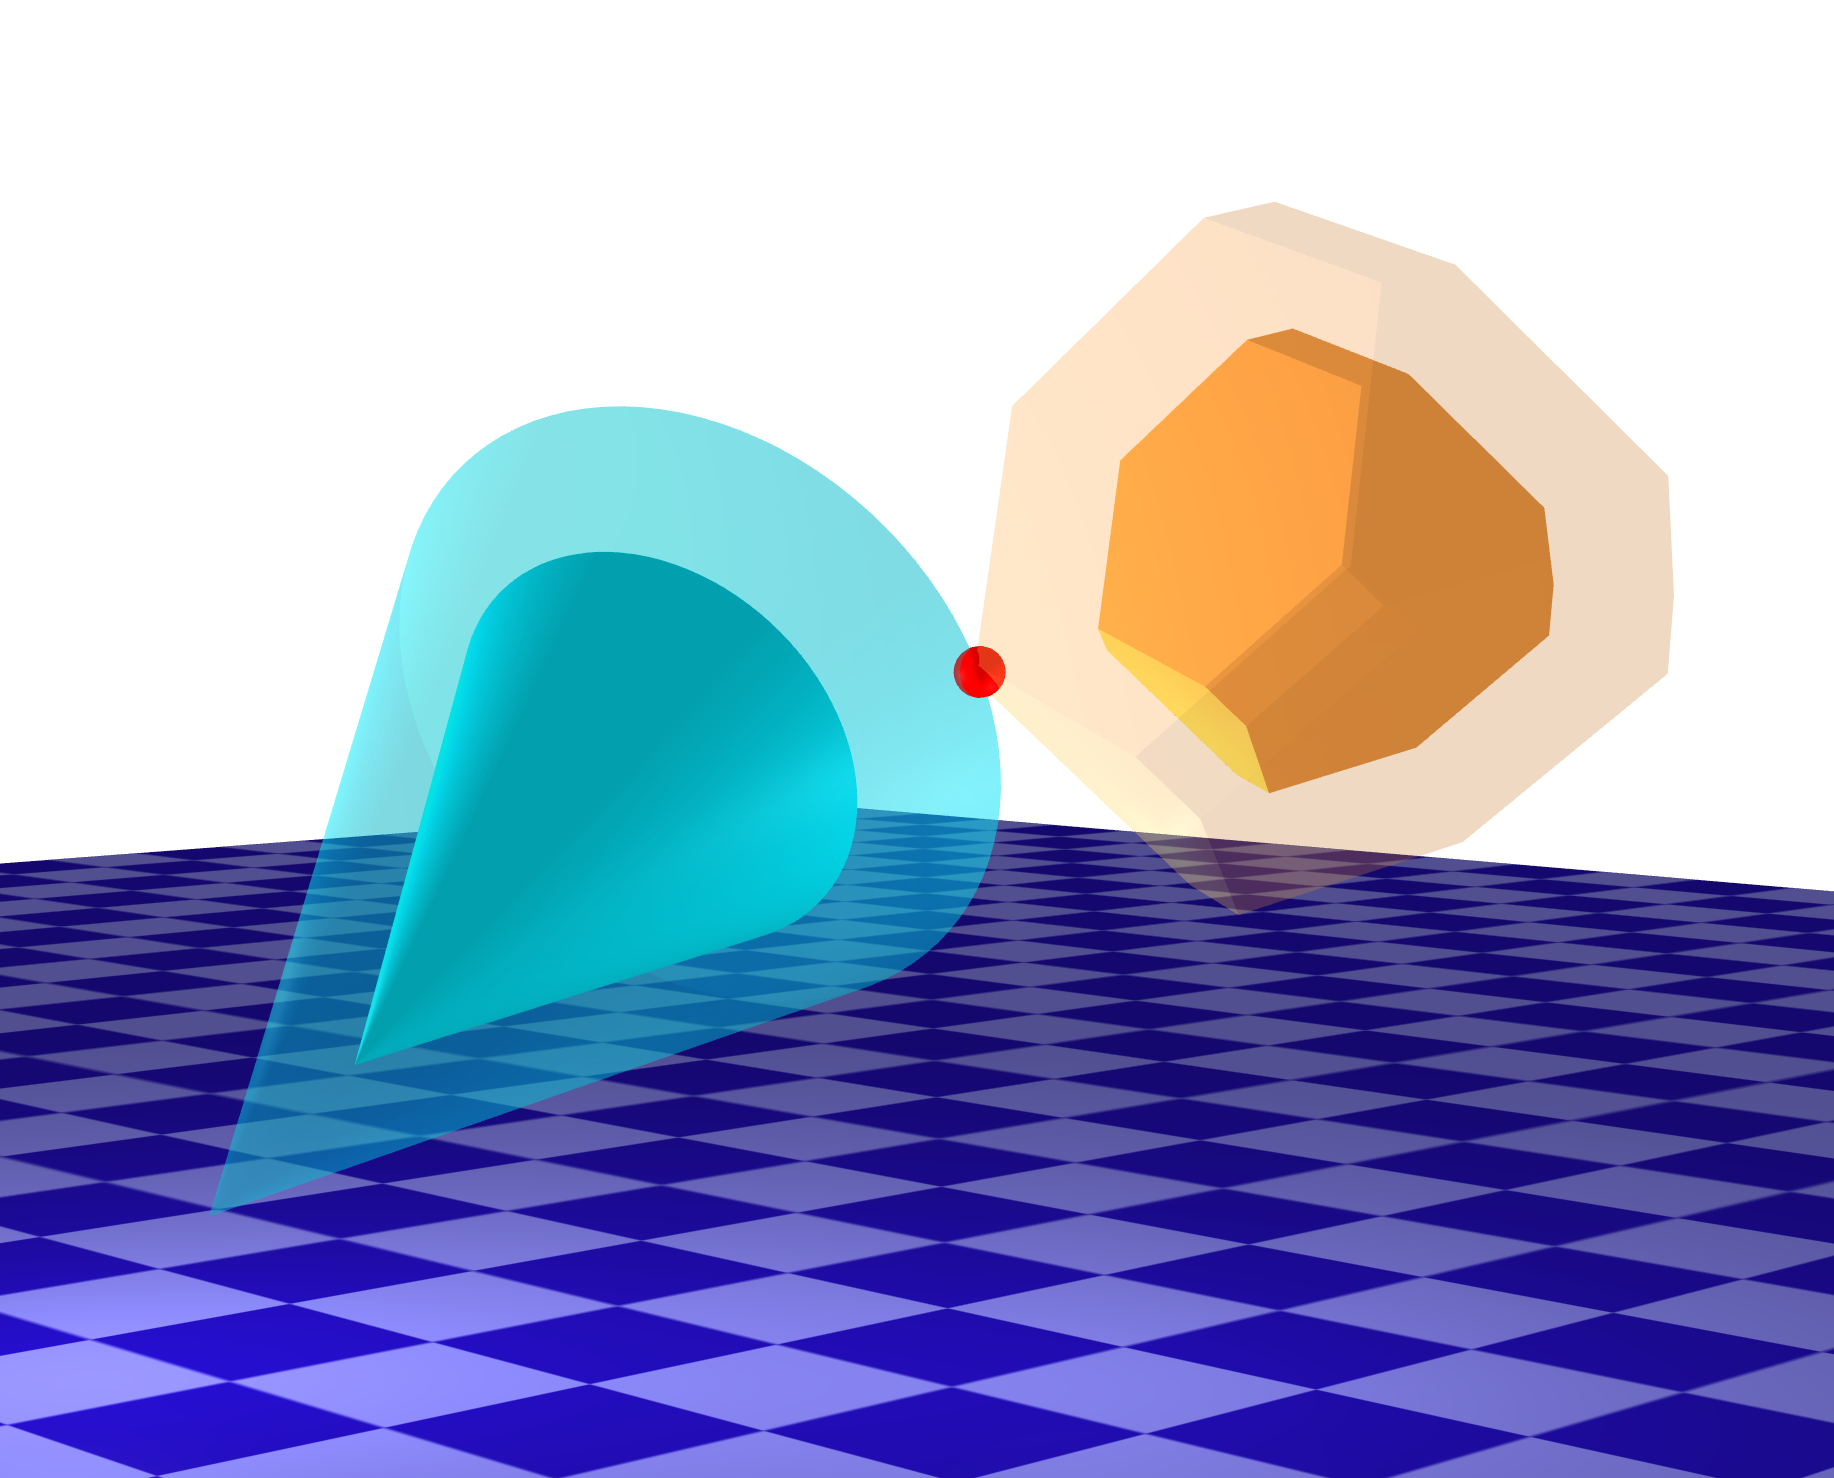
\includegraphics[width = 7.5cm]{figures/cone_poly_v9.png}}
\caption{Collision detection between a cone and a polytope. DCOL works by solving an optimization problem for the minimum scaling of each object that produces an intersection which, in this example, is greater than one, meaning there is no collision. The scaled objects are translucent and the intersection point between these scaled objects is shown in red.}
\label{fig:conepoly}
% \vspace{-10pt}
\end{figure}

The optimization problems produced by our formulation are bounded, feasible, and well-defined for all configurations of the primitives. Differentiable convex optimization allows the sensitivities of the solution to be calculated with respect to problem parameters with minimal added computation. This allows informative and smooth derivatives of the minimum scaling as well as the contact points with respect to the configurations of the primitives to be computed efficiently.

The ability to differentiate through our collision detection algorithm enables the inclusion of accurate collision information into gradient-based robotic simulation, control, and learning frameworks. We demonstrate this on several relevant robotics problems from trajectory optimization and contact physics. 
% \todo{We demonstrate this on several robotics problems, including...}

Our specific contributions in this paper are the following:
\begin{itemize}
    \item An optimization-based collision detection formulation between convex primitives that returns an informative collision metric even in the case of interpenetration
    \item Efficient differentiation of this optimization problem with respect to the configurations of each primitive 
    \item A fast and efficient open-source implementation of these algorithms built on a custom primal-dual interior-point solver
\end{itemize}

The paper proceeds by providing background on standard convex conic optimization and differentiation of conic optimization problems in Section \ref{sec:dcol:conic_opt}, a derivation of DCOL in Section \ref{sec:dcol:framework} with the corresponding constraints for each of the six convex primitives shown in Fig. \ref{fig_sim}, example use cases in trajectory optimization and contact physics in Section \ref{sec:dcol:examples}, and our conclusions in Section \ref{sec:dcol:conclusion}.

 \section{Background} \label{sec:dcol:conic_opt}
 The differentiable collision detection algorithm, DCOL, proposed in this paper is built on differentiable convex optimization. In this section, convex optimization with the relevant conic constraints is detailed, as well as a method for efficiently computing derivatives of these optimization problems with respect to problem parameters. 
 \subsection{Conic Optimization}
 DCOL formulates collision detection problems as a convex optimization problem with conic constraints \cite{boyd2004}. In standard form, these optimization problems have linear objectives and constraints of the following form:
 \begin{mini}
{x}{ c^Tx }{\label{conic_form}}{}
\addConstraint{h-Gx}{\in \mathcal{K},}%{k = 1,\ldots,N-1}
\end{mini}
where $x\in\R{n}$, $c \in \R{n}$, $G \in \R{m \times n}$, $h \in \R{m}$, and $\mathcal{K} = \mathcal{K}_1 \times \dotsm \times \mathcal{K}_N$ is a Cartesian product of $N$ proper convex cones. The optimality conditions for problem \ref{conic_form} are as follows:
\begin{align}
    c + G^Tz &= 0, \label{conic_kkt_1}\\
    h - Gx &\in \mathcal{K}, \label{conic_kkt_2}\\ 
    z &\in \mathcal{K}^*, \label{conic_kkt_3}\\ 
    (h-Gx) \circ z &= 0, \label{conic_kkt_4}
\end{align}
where a dual variable $z \in \R{m}$ is introduced, $\mathcal{K}^*$ is the dual cone, and $\circ$ is a cone product specific to each cone  \cite{vandenberghe}. 

The cones required for DCOL include the nonnegative orthant, denoted as $\mathbf{R}_+^m$, and the second-order cone, denoted as $\mathcal{Q}_m$. The nonnegative orthant contains any vector $s \in \mathbf{R}_+^m$ where $s \geq 0$, and the a second-order cone contains any vector $s \in \mathcal{Q}_m$ such that $\|s_{2:m}\|_2 \leq s_1$.

We develop a custom primal-dual interior-point solver for DCOL, with support for both of the relevant cones, based on the \textit{conelp} solver from \cite{vandenberghe}, with features taken from  \cite{domahidi2013a,nesterov1997,andersen2003,nesterov1998}.  The memory for this custom solver is entirely stack-allocated and is optimized for the small problems that DCOL creates, dramatically outperforming off-the-shelf primal-dual interior-point conic solvers like ECOS \cite{domahidi2013a} and Mosek \cite{mosekaps2014}.

\subsection{Differentiating Through a Cone Program}
Recent advances in differentiable convex optimization have enabled efficient differentiation through problems of the form \eqref{conic_form} \cite{agrawal2019,agrawal2019a,amos2019}.  Solutions to \eqref{conic_form} can be differentiated with respect to any parameters used in $c$, $G$, and $h$. %This allows for the construction of algorithms that solve problem \eqref{conic_form} while still remaining differentiable. 

At the core of differentiable convex optimization is the implicit function theorem. An implicit function $g:\R{a} \times \R{b} \rightarrow \R{a} $ is defined as:
\begin{align}
    g(y^*,\theta) &= 0 ,\label{ift:res}
\end{align}
for an equilibrium point $y^* \in \R{a}$, and problem parameters $\theta \in \R{b}$. Approximating \eqref{ift:res} with a first-order Taylor series results in: 
\begin{align}
    \frac{\partial g}{\partial y} \delta y + \frac{\partial g}{\partial \theta} \delta \theta &= 0 ,
\end{align}
which can be re-arranged to solve for the sensitivities of the solution with respect to the problem parameters:
\begin{align}
    \frac{\partial y}{\partial \theta} &= - \bigg( \frac{\partial g}{\partial y} \bigg)^{-1} \frac{\partial g}{\partial \theta}. \label{eq:ift}
\end{align}
By treating the optimality conditions in equations \eqref{conic_kkt_1} and \eqref{conic_kkt_4} as an implicit function at a primal-dual solution, the sensitivities of the solution with respect to the problem data can be computed. When the original optimization problem is solved using a primal-dual interior-point method as described in \cite{vandenberghe}, these derivatives can be computed after the solve without any additional matrix factorizations \cite{amos2019}.  This enables fast differentiation of conic programs that are fit for use in our differentiable collision detection algorithm.

In the case where only the gradient of the objective value $J$ with respect to the problem parameters $\theta$ is needed, the implicit function theorem is unnecessary. Instead, we need only the gradient of the Lagrangian for \eqref{conic_form}: 
\begin{align}
    \mathcal{L}(x,z,\theta) &= c(\theta)^Tx + z^T(G(\theta) x - h(\theta)),
\end{align}
where the problem matrices $c$, $h$, and $G$, are functions of the problem parameters $\theta$. Given a primal-dual solution $(x^*,z^*)$, the gradient of the objective value with respect to the problem parameters is simply the gradient of the Lagrangian with respect to these problem parameters, $ \nabla_\theta J = {\nabla_\theta \mathcal{L}(x^*,z^*,\theta)}$.
% In the case where only the gradient of the objective value $J \in \R{}$ of the optimization problem with respect to the problem parameters is needed, there is an alternative way of getting this derivative without requiring the solution to a linear system. The Lagrangian for a problem of the form \eqref{conic_form}, where the problem matrices are a function of parameters $\theta$ is the following:
% \begin{align}
%     \mathcal{L}(x,z,\theta) &= c(\theta)^Tx + z^T(h(\theta) - G(\theta) x).
% \end{align}
% To differentiate the optimal objective value with respect to these problem parameters, the following gradient is taken at primal and dual solutions $x^*$ and $z^*$
% \begin{align}
%     \nabla_\theta J &= {\nabla_\theta \mathcal{L}(x^*,z^*,\theta)}.
% \end{align}
This allows for a faster computation of this specific gradient without using the implicit function theorem.
\section{The DCOL Algorithm}\label{sec:dcol:framework}
\begin{figure}[!t]
\centering
\subfloat[]{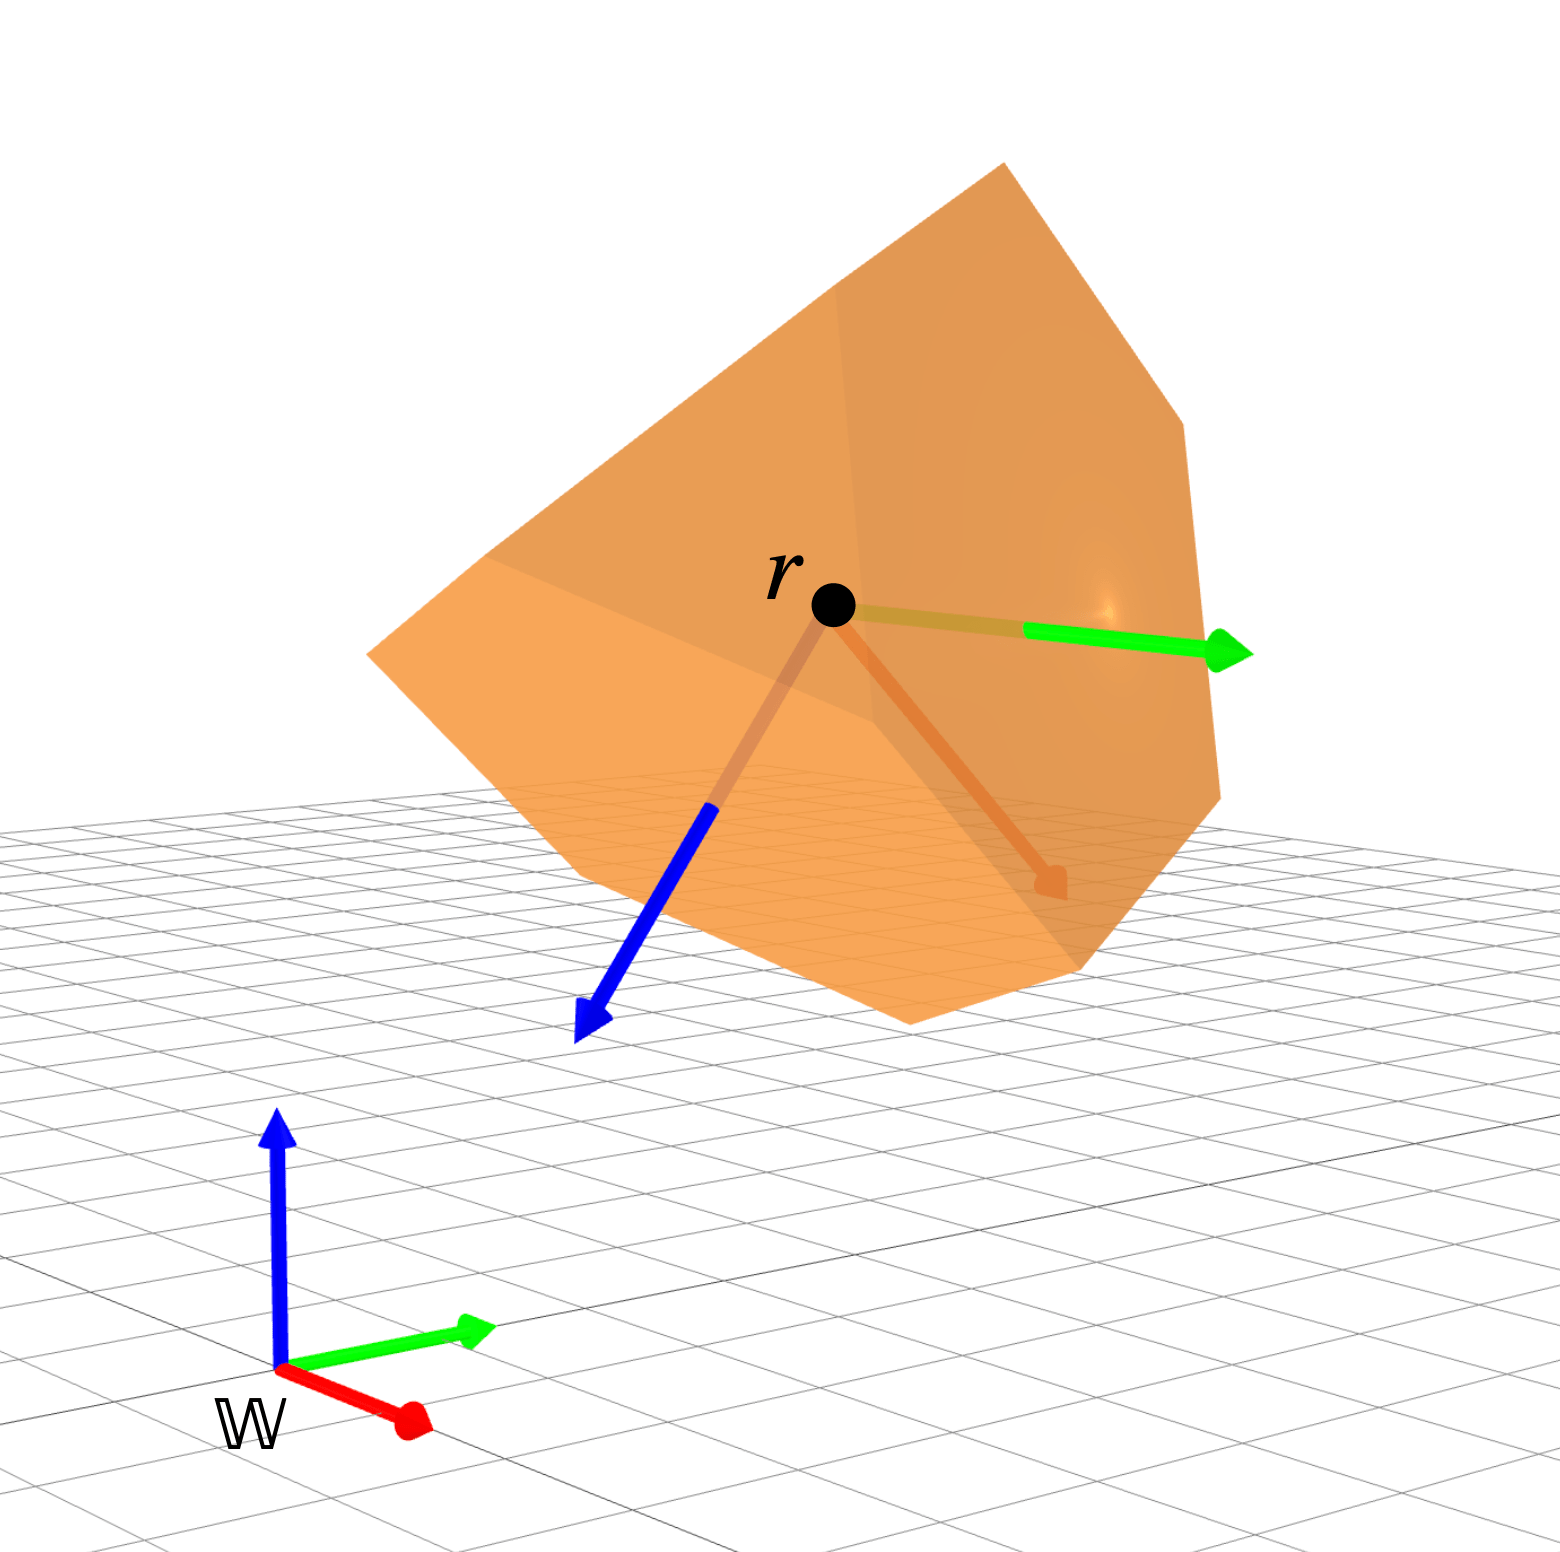
\includegraphics[width=1.8in]{figures/lineup_wire/polytope.png}%
\label{fig_polytope}}
\hfil
\subfloat[]{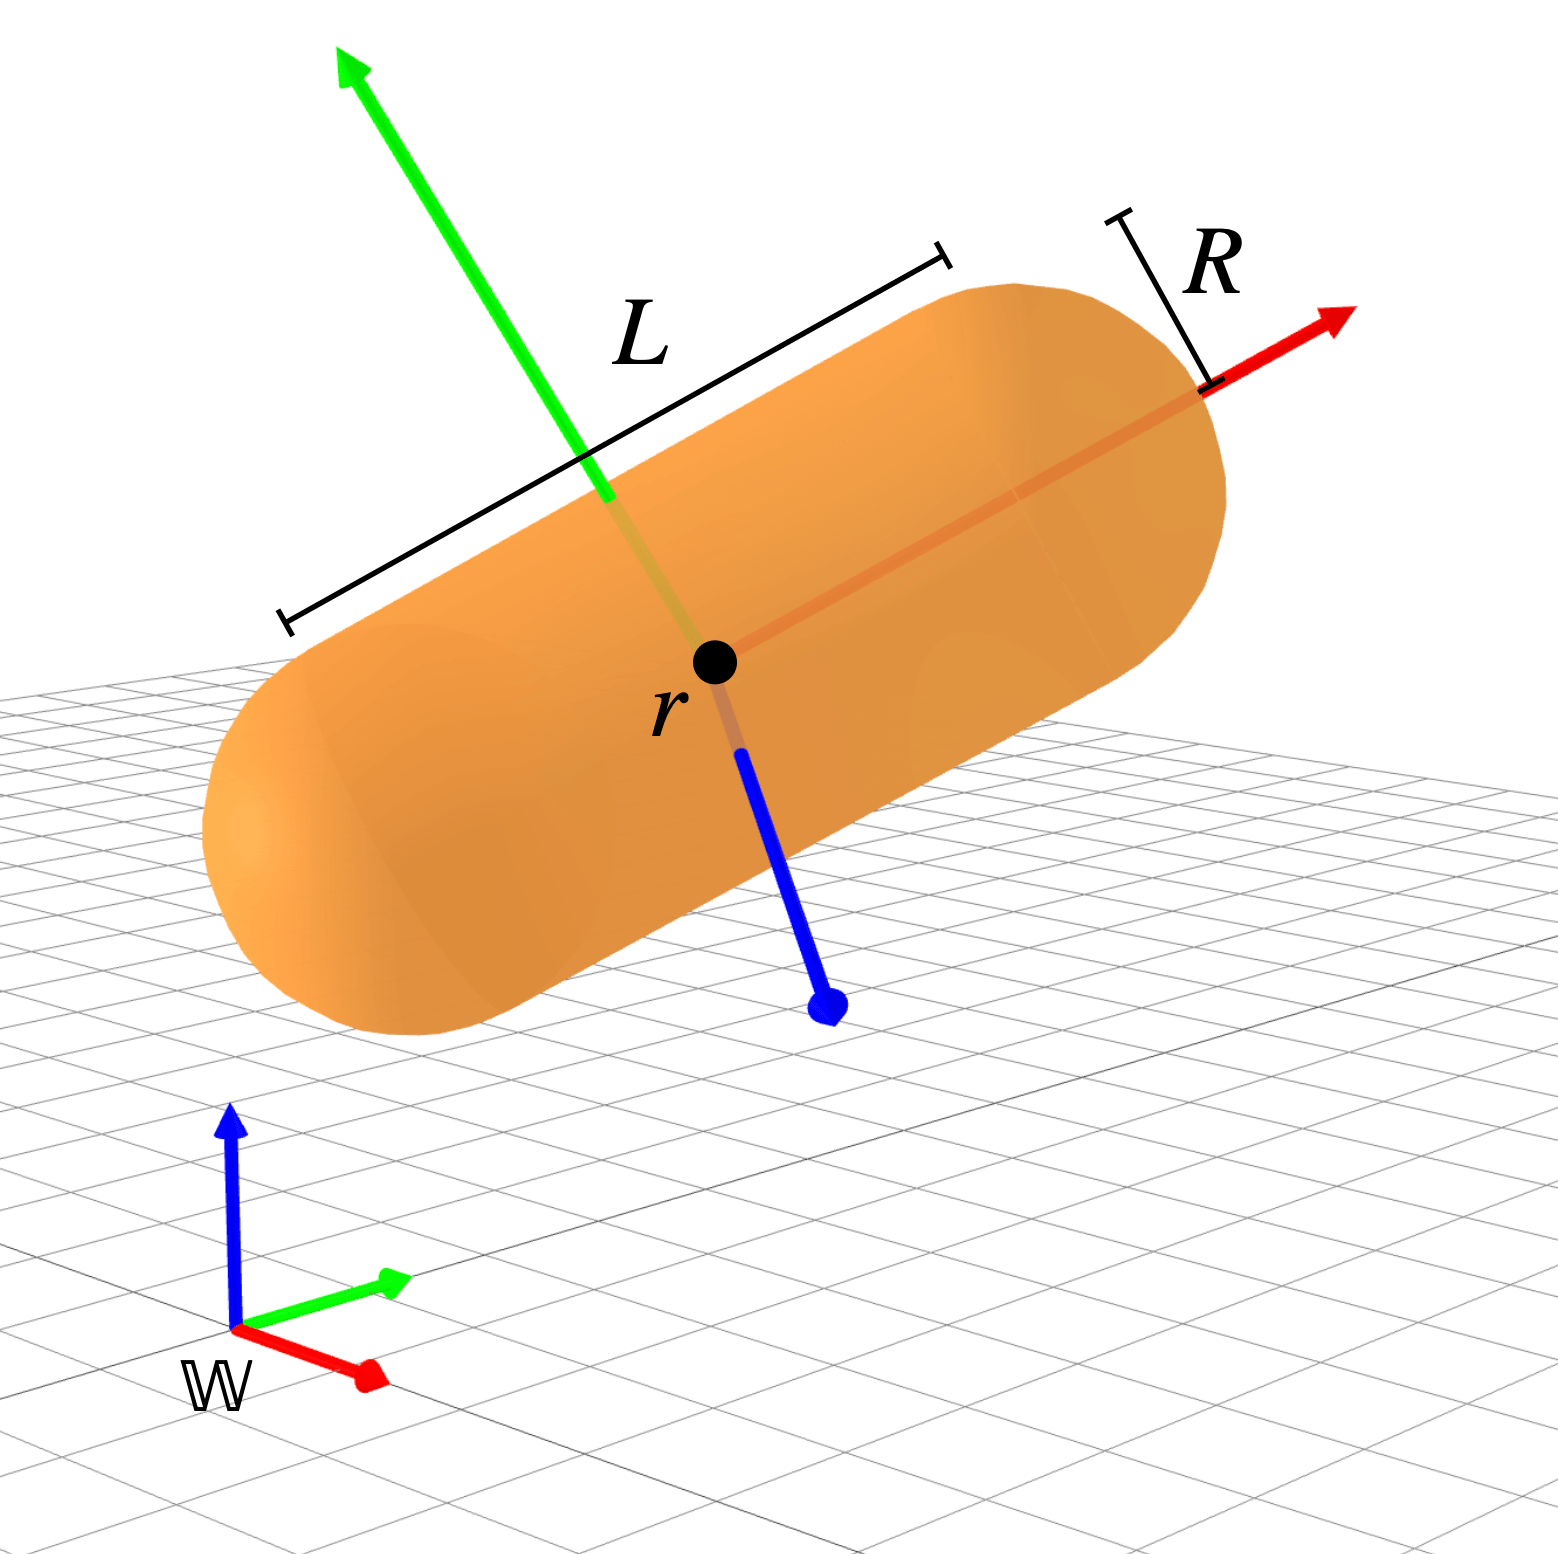
\includegraphics[width=1.8in]{figures/lineup_wire/capsule.png}%
\label{fig_capsule}}
\hfil
\subfloat[]{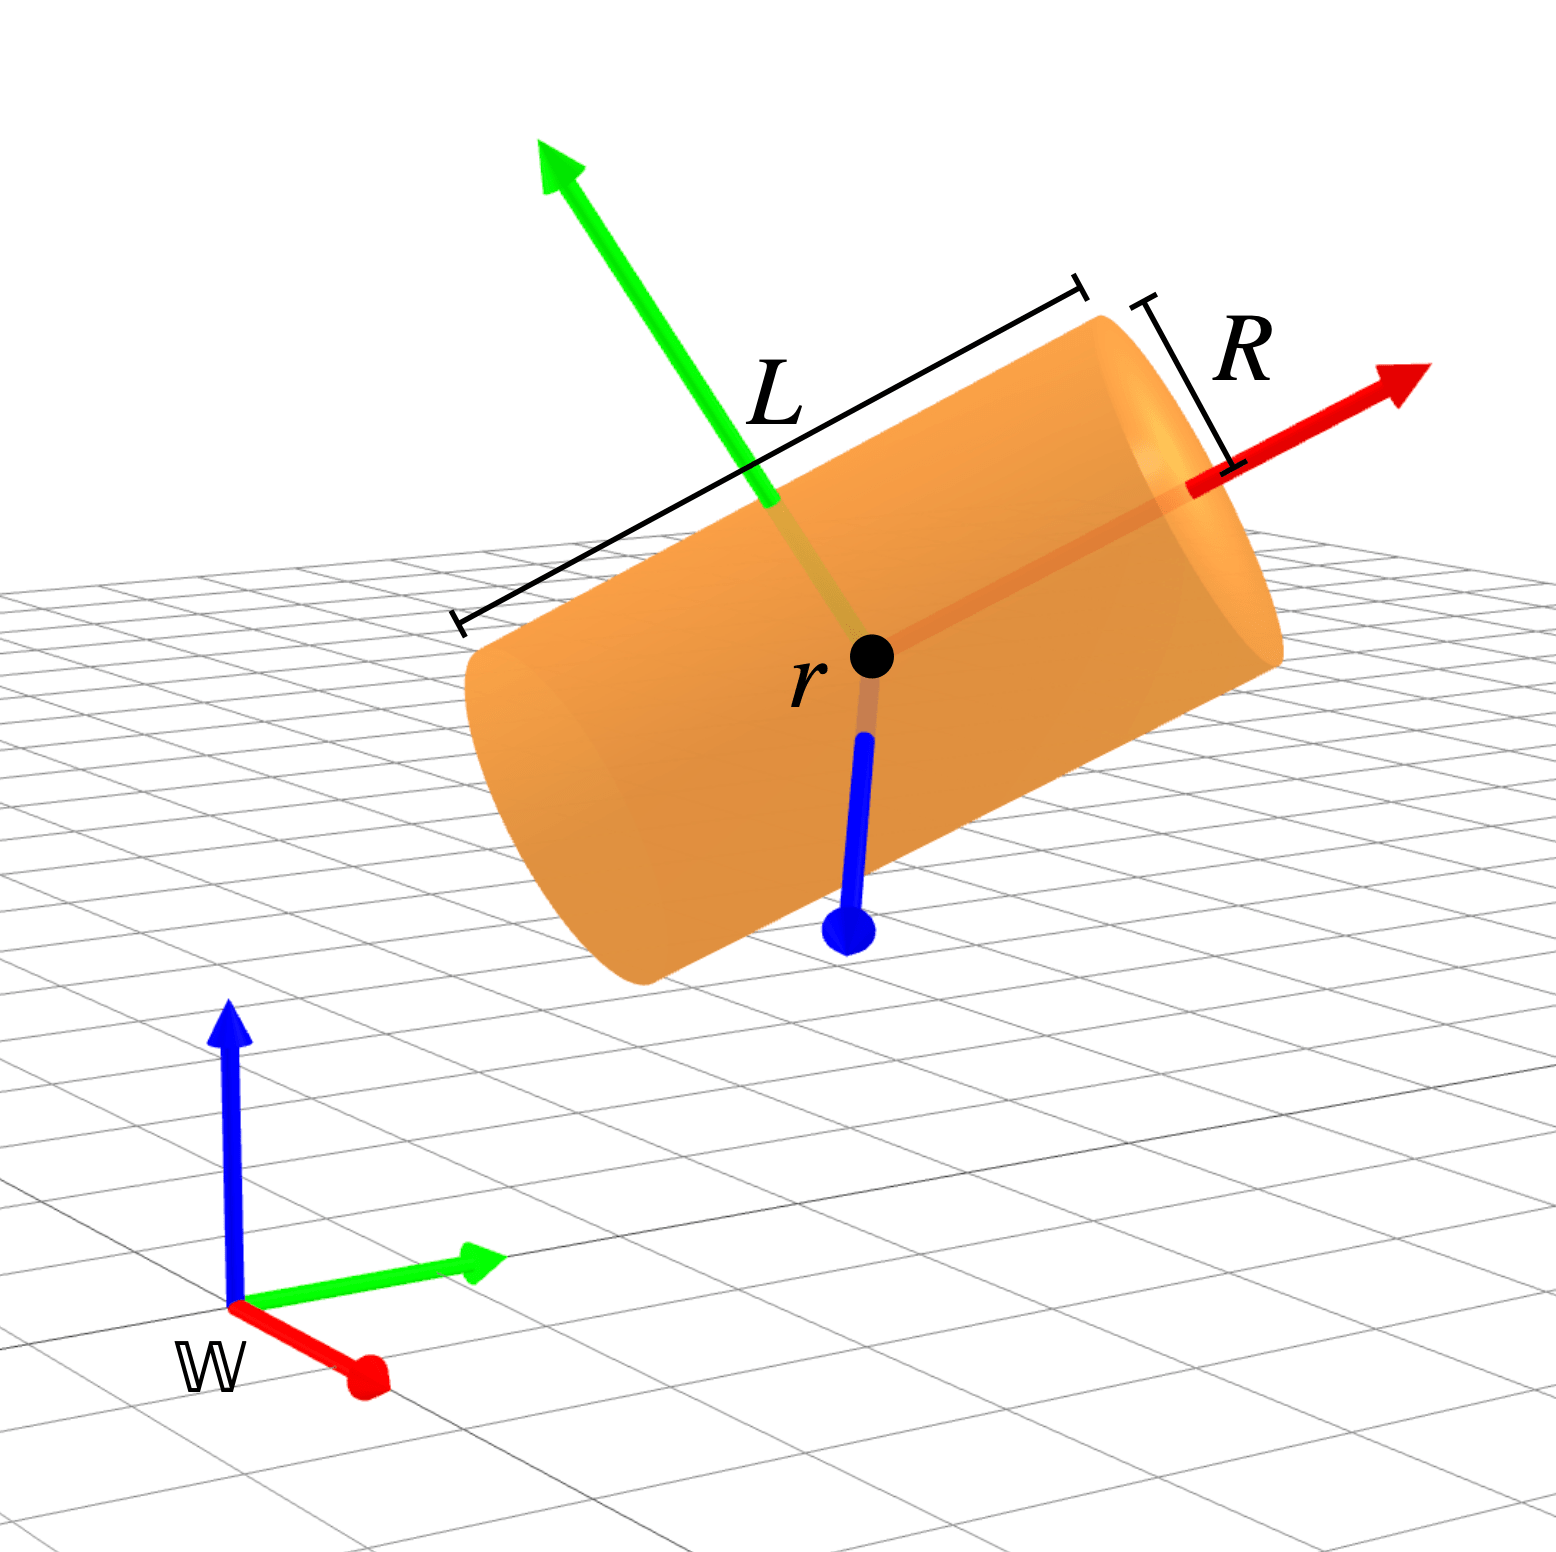
\includegraphics[width=1.8in]{figures/lineup_wire/cylinder.png}%
\label{fig_cyl}}
\hfil
\subfloat[]{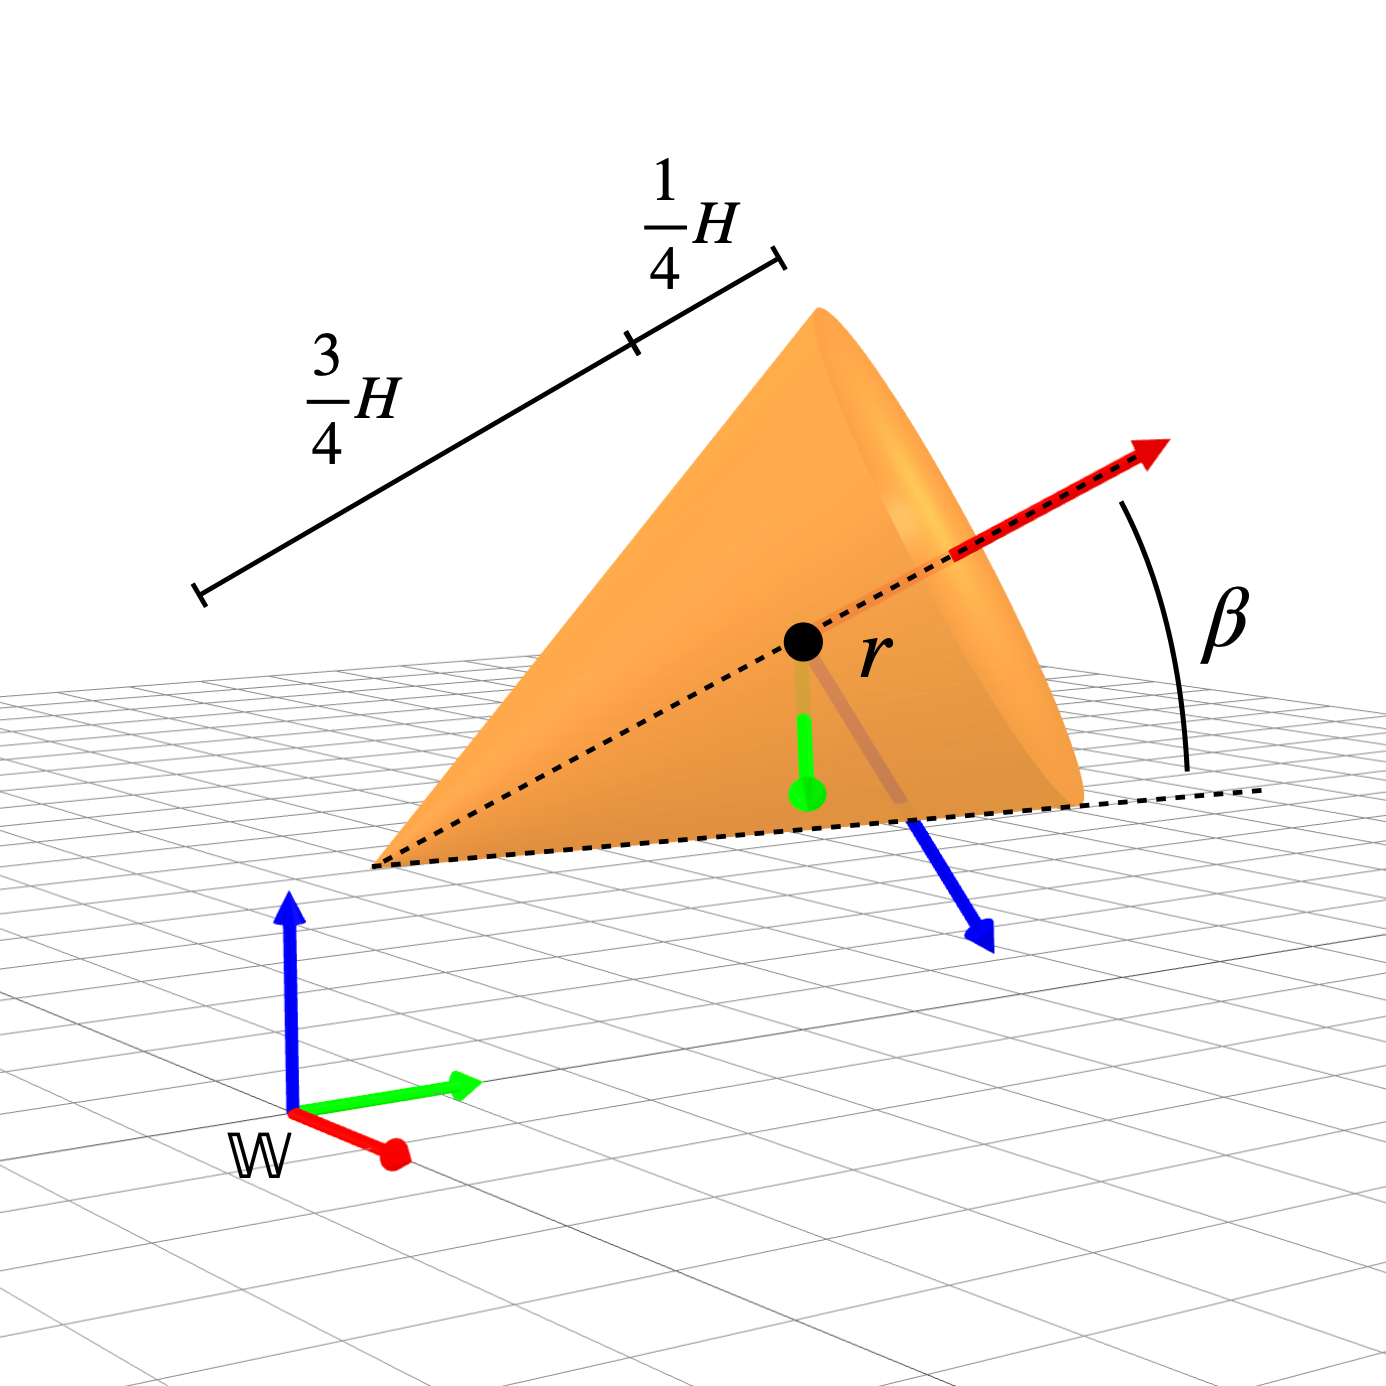
\includegraphics[width=1.8in]{figures/lineup_wire/cone.png}%
\label{fig_cone}}
\hfil
\subfloat[]{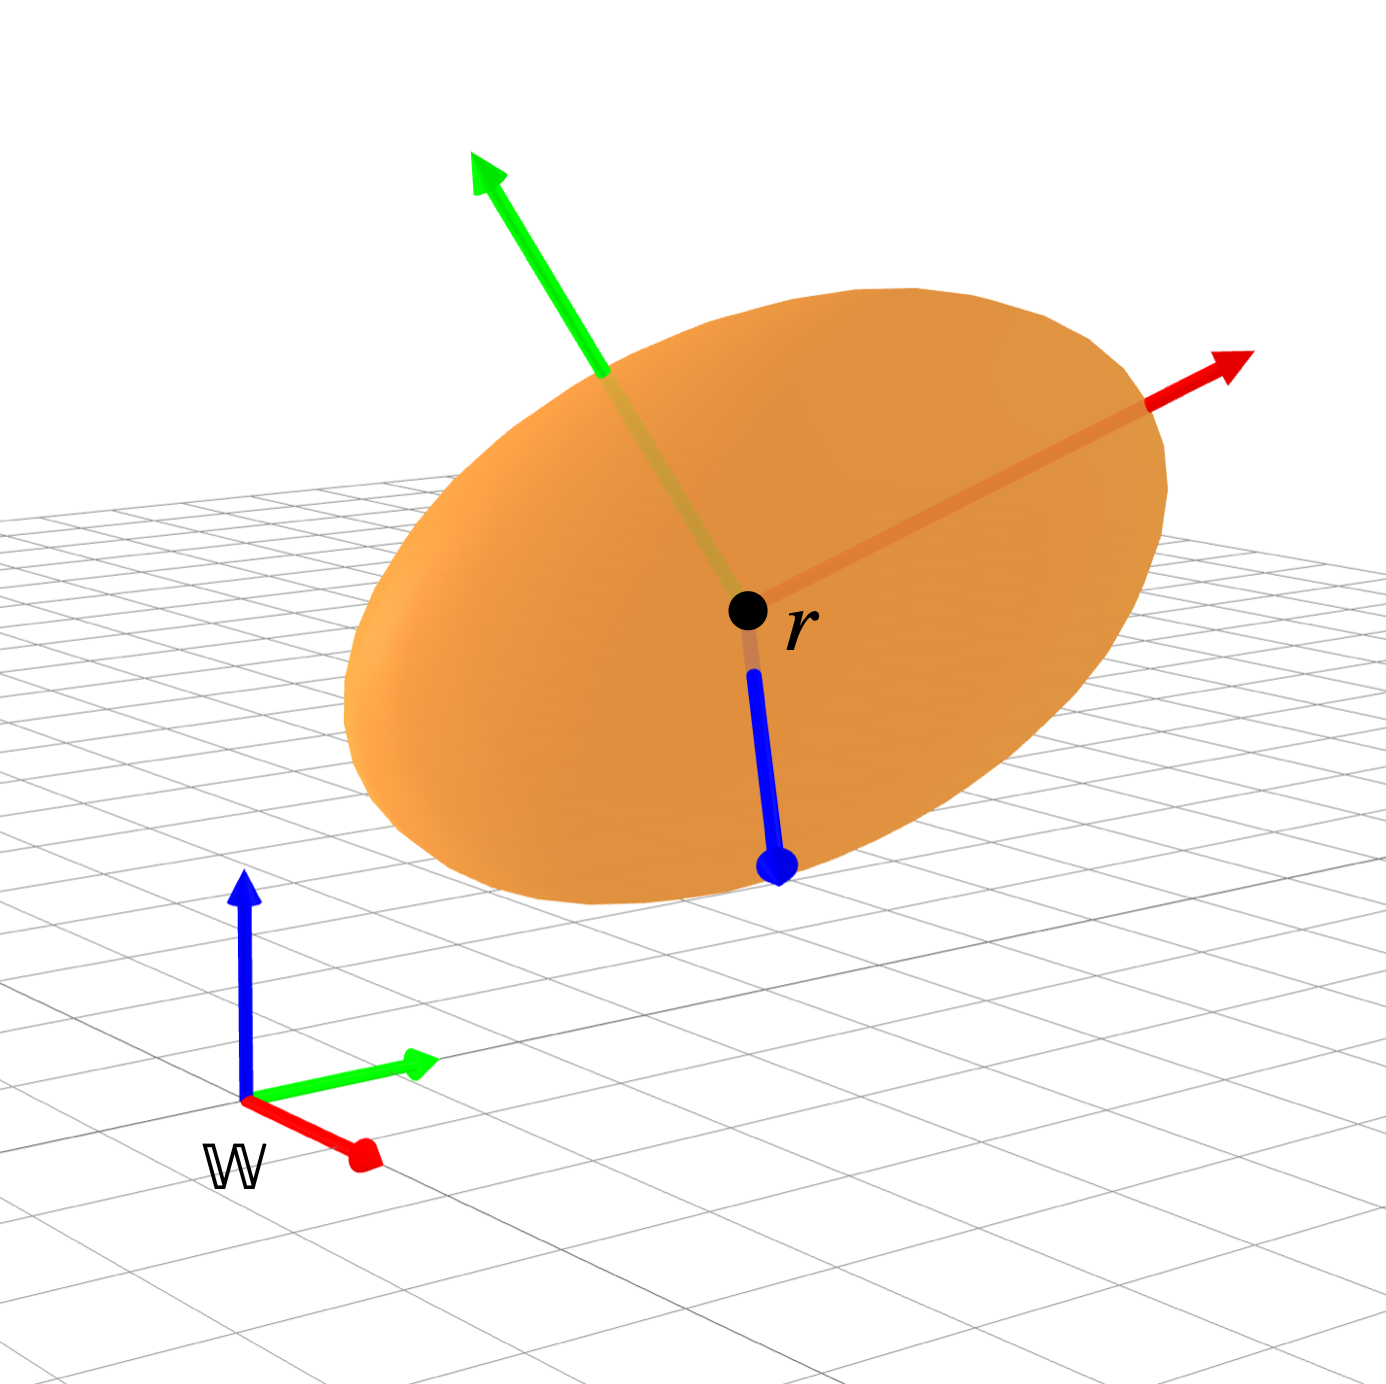
\includegraphics[width=1.8in]{figures/lineup_wire/ellipse.png}%
\label{fig_sphere}}
\hfil
\subfloat[]{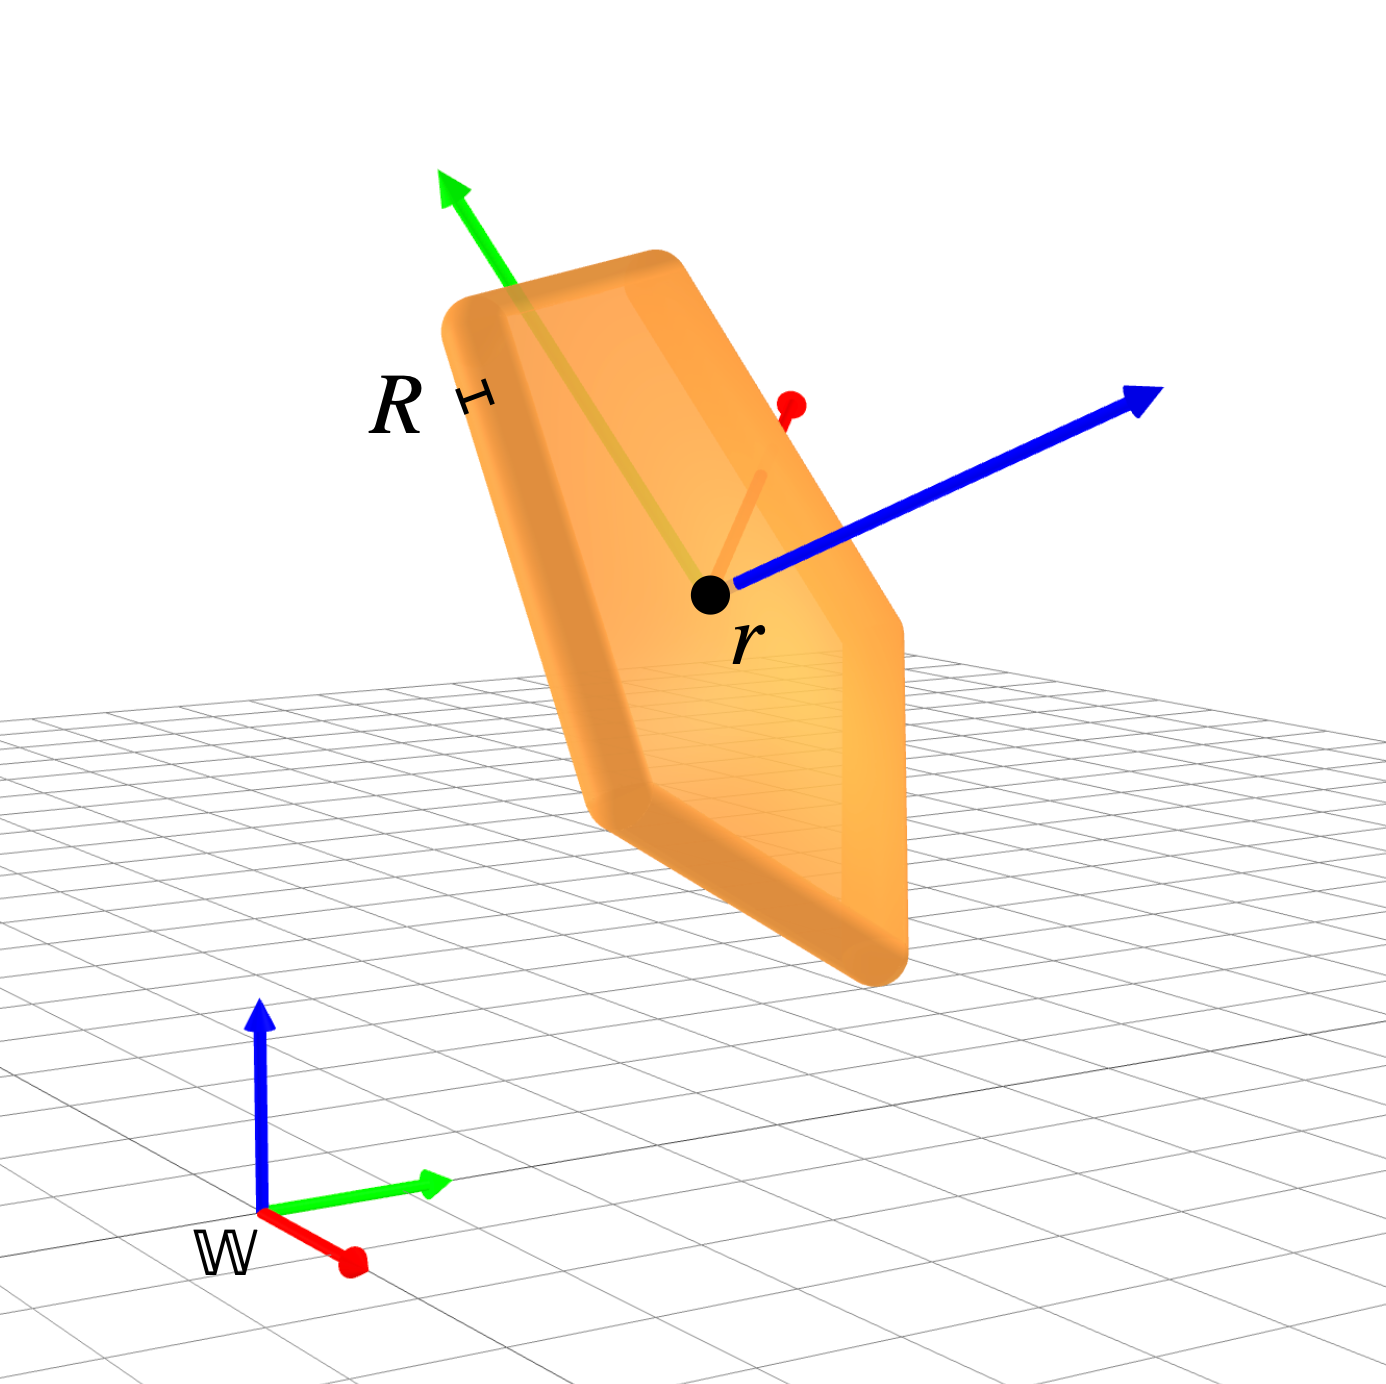
\includegraphics[width=1.8in]{figures/lineup_wire/polygon.png}%
\label{fig_polyg}}
\caption{Geometric descriptions of the six primitive shapes that are compatible with this differentiable collision detection algorithm. These shapes include a polytope (a), capsule (b), cylinder (c), cone (d), ellipsoid (e), and padded polygon (f). Collision information including the collision status as well as the contact points can be computed between any of two of these primitives using DCOL.}
\label{fig_sim}
\end{figure}
This section details how DCOL computes collision information between two convex primitives.  The core part of this framework is an optimization problem that solves for a minimum uniform scaling $\alpha \in \R{}$ applied to both objects that result in an intersection. In the case where there is no collision between the two objects, the minimum scaling is greater than one, and when there is interpenetration, the minimum scaling is less than one. Because of this, we find the minimum scaling $\alpha$ is a better collision metric than the closest distance between the primitives, allowing for the straightforward description of collision constraints that are agnostic of interpenetration.  All steps in the creation and solving of this optimization problem are fully differentiable, and average timing results for computing both solutions and derivatives are provided in Table \ref{speed_table} as an average over each primitive.
\begin{table}[!t]
\centering 
\caption{Average DCOL Computation Times}
\begin{tabular}{c c c c c c c}
		\toprule
	                 &
                  \textbf{polyt.} & 
                  \textbf{caps.} & 
                  \textbf{cyl.} & 
                  \textbf{cone} & 
                  \textbf{ellips.} & 
                  \textbf{polyg.} \\
		\toprule
        evaluate & 5.9 $\mu$s &  8.5 $\mu$s     & 8.4 $\mu$s     & 5.0 $\mu$s     & 6.8 $\mu$s        & 9.4 $\mu$s       \\
differentiate &  1.4 $\mu$s                        &  1.4 $\mu$s     &  1.6 $\mu$s    &  1.3 $\mu$s    &   1.3 $\mu$s      &  1.7 $\mu$s      \\
		\toprule
\end{tabular}
\label{speed_table}
\end{table}
\subsection{Optimization Problem}
Scaled convex primitives are described as a set $S(\alpha)$, which is a specific instance of the primitive scaled by some $\alpha$. A point $x\in \R{3}$ is said to be in the set $x \in S(\alpha)$ if $x$ is within the scaled primitive. This notation allows for the following formulation of the optimization problem:
 \begin{mini}
{x, \alpha}{ \alpha }{\label{dcd}}{}
\addConstraint{x}{\in \mathcal{S}_1(\alpha)}
\addConstraint{x}{\in \mathcal{S}_2(\alpha)}
\addConstraint{\alpha}{\geq 0,}
\end{mini}
where the minimum scaling $\alpha$ is computed such that $x$ is in the interior of both of the scaled primitives, making $x$ an intersection point. This optimization problem is convex, bounded, and feasible for all of the primitives described in this paper. The boundedness comes from the constraint $\alpha \geq 0$, and the guarantee of feasibility comes from the fact that each object is uniformly scaled, so that in the limit $\alpha \rightarrow \infty$ each shape will encompass the entirety of $\R{3}$, guaranteeing an intersection between objects. Another benefit to this problem formulation is that the only time the minimum scaling $\alpha = 0$ is when the origins of the two objects are coincident, in which the problem and its derivatives are still well defined.
\subsection{Primitives}
This section details the constraints that define set membership for each of the six scaled primitives.  Each object is defined with an attached body reference frame $\mathbb{B}$ with an origin $r\in\R{3}$ expressed in a world frame $\mathbb{W}$. The uniform scaling of these objects is always centered about this position $r$, and when the scaling parameter $\alpha$ is $0$, the object is simply a point centered at $r$.  The orientation of an object is defined by a rotation matrix ${}^\mathbb{W} Q {}^\mathbb{B} \in \R{3 \times 3}$ relating the world frame to the object-fixed body frame, denoted as $Q$ for shorthand.  For each primitive, the constraints are also explicitly written in standard conic form for direct inclusion in our custom conic solver in the form of \eqref{conic_form}, where $h - Gx \in \mathcal{K}$.
\subsubsection{Polytope}
A polytope is a convex shape in $\R{3}$ defined by a set of halfspace constraints, an example of which is shown in Fig. \ref{fig_polytope}. This polytope is described as the set of points $w \in \R{3}$ such that  $Aw\leq b$ for $w$ expressed in $\mathbb{B}$, where $A \in \R{m \times 3}$ and $b \in \R{m}$ represent the $m$ halfspace constraints comprising the polytope. This polytope can be scaled by $\alpha$, resulting in the following constraint for $x$ to be inside the polytope:
\begin{align}
    AQ^T (x - r) &\leq \alpha b.
\end{align}
The scaling parameter $\alpha$ scales the vector $b$, resulting in uniform scaling of all halfspace constraints and subsequent uniform scaling of the polytope. This constraint in standard form is the following: 
\begin{align}
   AQ^Tr  - \begin{bmatrix} A Q^T & -b \end{bmatrix} \begin{bmatrix} x \\ \alpha \end{bmatrix} &\in \mathbf{R}_+ .
\end{align}
\subsubsection{Capsule}
A capsule can be defined by the set of points within some radius $R$ of a line segment, as shown in Fig. \ref{fig_capsule}.  This internal line segment is along the $x$ axis of the attached reference frame $\mathbb{B}$, and the end points of this line segment are some distance $L$ apart. The scaled constraints for this primitive are that the point $x$ must be within a scaled radius of the line segment, where the distance of the endpoints of the line segment from $r$ is also scaled: 
\begin{align}
    \| x - (r + \gamma \hat{b}_x) \|_2 &\leq \alpha R, \label{cyl_con_1}\\ 
    -\alpha \frac{L}{2} \leq \gamma &\leq \alpha \frac{L}{2},\label{cyl_con_2}
\end{align}
where $\hat{b}_x = Q [1,0,0]^T$, and $\gamma \in \R{}$ is a slack variable.  These constraints contain a linear inequality and one second-order cone constraint, shown here in standard form:
\begin{align}
    \begin{bmatrix} 0 \\ 0 \end{bmatrix} - \begin{bmatrix} 0_{1 \times 3} & -L/2 & 1 \\ 0_{1 \times 3} & -L/2 & -1 \end{bmatrix} \begin{bmatrix} x \\ \alpha \\ \gamma \end{bmatrix} &\in \mathbf{R}_+^2, \label{eq:std_caps1}\\ 
    \begin{bmatrix}0 \\ -r  \end{bmatrix}  - \begin{bmatrix} 0_{1 \times 3} & -R & 0 \\ -I_3 & 0_{3 \times 1} & \hat{b}_x  \end{bmatrix} \begin{bmatrix} x \\ \alpha \\ \gamma \end{bmatrix} &\in \mathcal{Q}_4. \label{eq:std_caps2}
\end{align}
\subsubsection{Cylinder}
The description of a cylinder is shown in Fig. \ref{fig_cyl}, with an orientation, a radius $R$, and a length $L$. The constraints for this primitive are the same as for the capsule in equations \eqref{cyl_con_1} and \eqref{cyl_con_2}, with the introduction of two new scaled halfspace constraints that give the cylinder its flat ends:
\begin{align}
    [x - (r - \alpha \frac{L}{2} \hat{b}_x)]^T \hat{b}_x &\geq 0, \\ 
    [x - (r + \alpha \frac{L}{2} \hat{b}_x)]^T \hat{b}_x &\leq 0.
\end{align}
These constraints in standard form include those shown in equations \eqref{eq:std_caps1} and \eqref{eq:std_caps2} with the following addition:
\begin{align}
    \begin{bmatrix}  -\hat{b}_x^Tr \\ \phantom{-}\hat{b}_x^Tr \end{bmatrix} - \begin{bmatrix}  -\hat{b}_x^T & -L/2 & 0 \\ \phantom{-} \hat{b}_x^T & -L/2 & 0\end{bmatrix} \begin{bmatrix} x \\ \alpha \\ \gamma \end{bmatrix} &\in \mathbf{R}_+^2.
\end{align}
\subsubsection{Cone}
As shown in Fig. \ref{fig_cone}, a cone can be described with a height $H$, and a half angle $\beta$. The origin of the object-fixed frame $r$ is one-quarter of the way from the flat face to the point of the cone, and $\alpha$ scales the distance of these two ends from the center point $r$:
\begin{align}
    \|\tilde{x}_{2:3}\|_2 &\leq \tan(\beta) \tilde{x}_1, \\ 
    (x - r - \alpha \frac{H}{4} \hat{b}_x)^T \hat{b}_x &\leq 0 ,
\end{align}
where $\tilde{x} = Q^T  (x - r + \alpha \frac{3H}{4} \hat{b}_x)$.  These constraints in standard form are:
\begin{align}
    \hat{b}_x^Tr - \begin{bmatrix} \hat{b}_x^T  & -H/4  \end{bmatrix} \begin{bmatrix} x \\ \alpha \end{bmatrix} &\in \mathbf{R}_+^m, \\ 
    -EQ^Tr  - \begin{bmatrix} -EQ^T & v \end{bmatrix} \begin{bmatrix} x \\ \alpha \\  \end{bmatrix} &\in \mathcal{Q}_3,
\end{align}
where $E = \operatorname{diag}(\tan \beta,1,1)$ and $v = (-\frac{3H}{4} \tan \beta,0,0)$.
% \begin{align}
% E &= \operatorname{diag}(\tan(\beta),1,1), \\ v &= [-3\tan(\beta)H/4,0,0]^T
% \end{align}
% \todo{switch these to display mode (not inline) if you have space left at the end of the paper}.
\subsubsection{Ellipsoid}
An ellipsoid, shown in Fig. \ref{fig_sphere}, can be described by a quadratic inequality $x^TPx \leq 1$, where $P\in \mathbf{S}^n_{++}$ is strictly positive definite and has an upper-triangular Cholesky factor $U \in \R{n \times n}$ \cite{boyd2004}. From here, a scaled ellipsoid with arbitrary position and orientation can be expressed in the following way:
\begin{align}
    \|U Q^T (x - r)\|_2 \leq \alpha,
\end{align}
where a sphere of radius $R$ is just a special case of an ellipsoid with $P = I/R^2$. These constraints can be written in standard form as:
\begin{align}
   \begin{bmatrix} 0 \\ -UQ^Tr \end{bmatrix} - \begin{bmatrix} 0_{1 \times 3} & -1 \\ -UQ^T & 0_{3 \times 1} \end{bmatrix} \begin{bmatrix} x \\ \alpha \end{bmatrix} &\in \mathcal{Q}_4 .
\end{align}
\subsubsection{Padded Polygon}
A ``padded" polygon is defined as the set of points within some radius $R$ of a two-dimensional polygon. Shown in Fig. \ref{fig_polyg}, the first two basis vectors of $\mathbb{B}$ span the polygon, and the polygon itself is defined with a slack variable $y \in \R{2}$, and $Cy\leq \alpha d$, where $C \in \R{m \times 2}$, and $d \in \R{m}$, describe the $m$ halfspace constraints for the polygon. This polygon is scaled in the same fashion as the polytope, and results in the following constraints:
\begin{align}
    \| x - (r + \tilde{Q} y)\|_2 &\leq \alpha R, \\ 
    Cy &\leq \alpha d,
\end{align}
where $\tilde{Q} \in \R{3\times 2}$ is the first two columns of $Q$. These constraints can be represented in standard form as the following:
\begin{align}
    0_{m} - \begin{bmatrix} 0_{m \times 3} & -d & C  \end{bmatrix} \begin{bmatrix} x \\ \alpha \\ y\end{bmatrix} &\in \mathbf{R}_+^m, \\
   \begin{bmatrix} 0 \\ -r \end{bmatrix} - \begin{bmatrix} 0_{1 \times 3} & -R & 0_{1 \times 2} \\ -I_3 & 0_{3 \times 1} & \tilde{Q} \end{bmatrix} \begin{bmatrix} x \\ \alpha \end{bmatrix} &\in \mathcal{Q}_4.
\end{align}
\subsection{Contact Points and Minimum Distance}
While the computation of contact points and minimum distance between primitives is not needed for any of the examples in Section \ref{sec:dcol:examples}, they are easy to compute with DCOL if desired. The intersection point on the two scaled primitives is referred to as $x^*$, but unless $\alpha^*=1$, this point does not exist on the surface of the primitives. The corresponding contact point for primitive $i$, $p_i \in \R{3}$, is calculated using the optimal $x^*$ and $\alpha^*$ from \eqref{dcd} as
\begin{align}
    p_i &= r_i + \frac{x^* - r_i}{\alpha^*},
\end{align}
% Which can be differentiated with respect to an arbitrary variable $y$ in the following manner:
% \begin{align}
%     \jac{p}{y} &= \jac{r_i}{y} + \frac{1}{\alpha^2} \bigg[ \alpha \bigg( \jac{x}{y} - \jac{r_i}{y} \bigg) - (x - r_i)\jac{\alpha}{y} \bigg].
% \end{align}
where the intersection point between the scaled primitives is simply scaled back to each unscaled primitive. The distance between these points can also be calculated as follows:
\begin{align}
    \|d\|_2 = \|p_1 - p_2\|_2 &= \|r_1 - r_2 + \frac{r_2 - r_1}{\alpha}\|_2.
\end{align}
% which is again differentiable with the following:
% \begin{align}
%     \jac{\|d\|}{y} = \frac{1}{\|d\|}d^T\jac{d}{y},
% \end{align}
% where
% \begin{align}
% \jac{d}{y} &= \jac{r_1}{y} - \jac{r_2}{y} + \frac{1}{\alpha^2} \bigg[ \alpha \bigg( \jac{r_2}{y} - \jac{r_1}{y} \bigg) - (r_2 - r_1)\jac{\alpha}{y} \bigg]
% \end{align}
Both of these operations are fully differentiable given the derivatives from DCOL, allowing for the calculation of the sensitivities of the contact points with respect to the configurations of the primitives. 
\begin{figure}[t!]
    \centering
    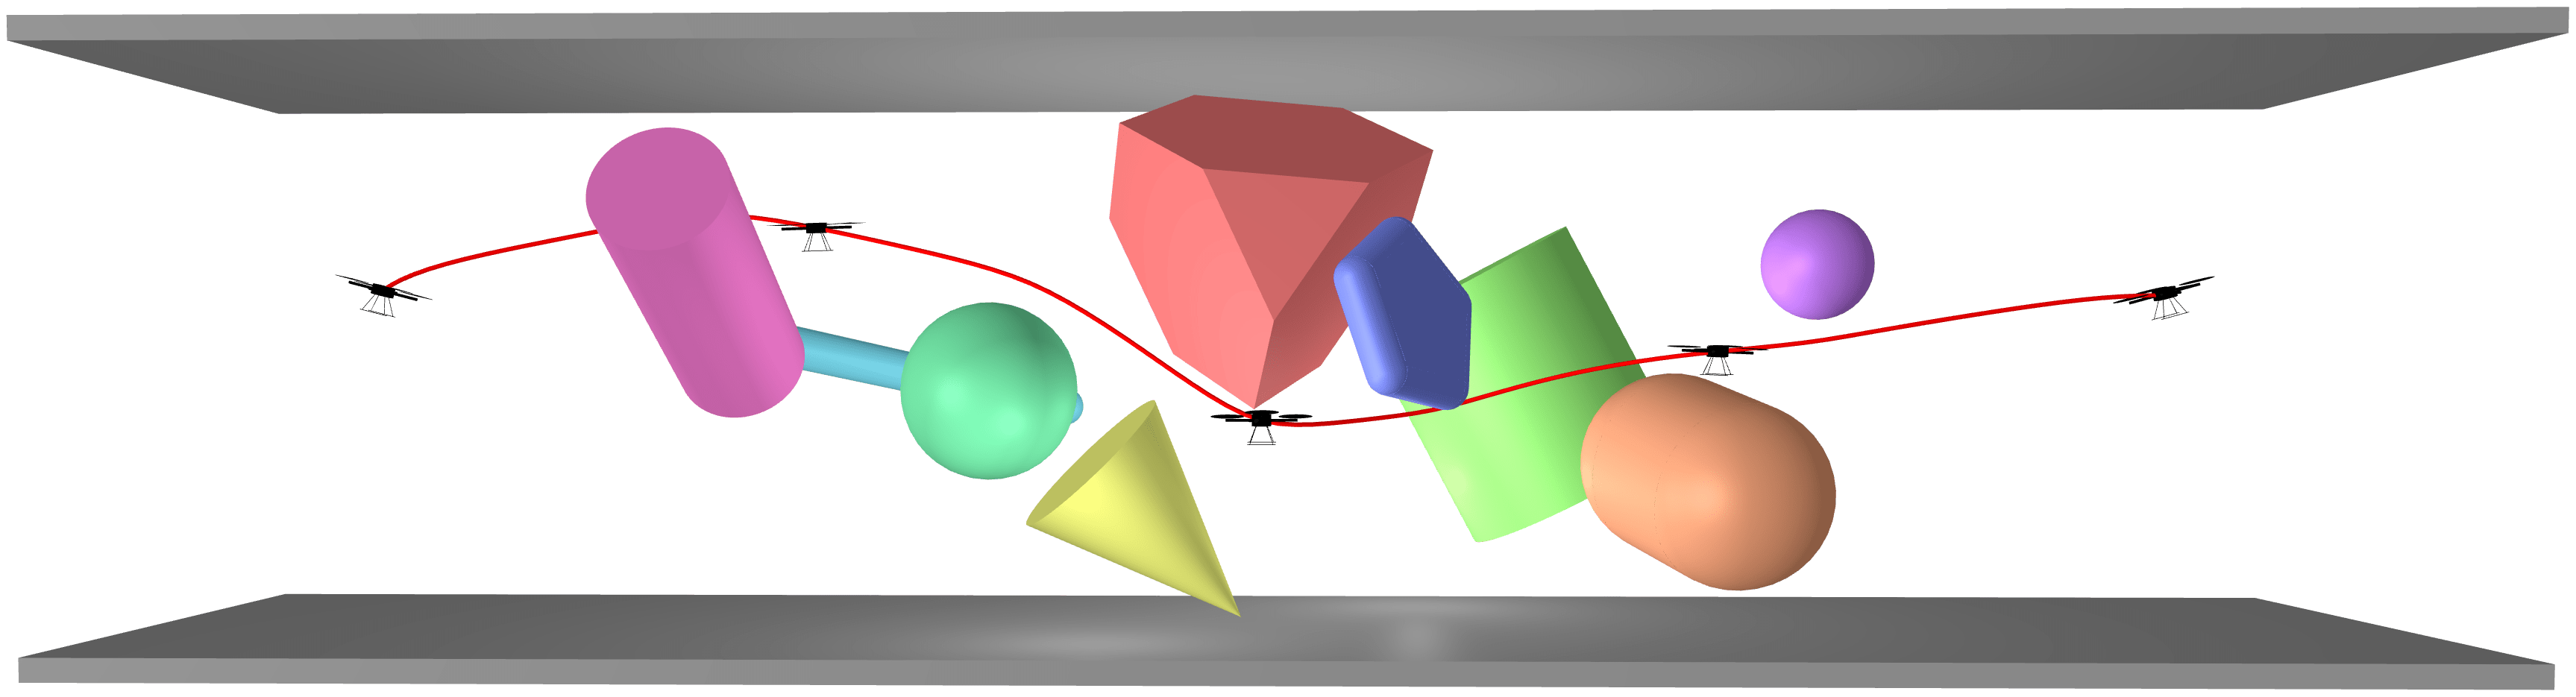
\includegraphics[width=.9\textwidth]{figures/hallway_v5.png}
    \caption{Trajectory optimization for a 6-DOF quadrotor as it moves from left to right through a cluttered hallway. The collision constraints were represented with DCOL, and the trajectory optimizer was initialized with a static hover at the initial condition.}
    \label{fig:hallway}
\end{figure}
\section{Examples}\label{sec:dcol:examples}
In this section, we demonstrate the utility of differentiable collision detection in trajectory optimization problems where contact is to be avoided, and in physics simulation with contact where exact and differentiable collision information is required.  In both of these applications, a collision constraint $\alpha \geq 1$ is used to enforce no interpenetration between each pair of primitives, where $\alpha$ is the minimum scaling from DCOL.
\subsection{Trajectory Optimization}
Trajectory optimization is a powerful tool in motion planning and control, where a numerical optimization problem is formulated to solve for a constrained trajectory that minimizes a cost function.  A generic trajectory optimization problem with collision avoidance constraints from DCOL is as follows:
 \begin{equation}
	\begin{array}{ll}
	\underset{x_{1:N},u_{1:N-1}}{\mbox{minimize }} & \ell_N(x_N) + \sum_{k=1}^{N-1} \ell_k(x_k,u_k) \\
	\mbox{subject to } & x_{k+1} = f_k(x_k,u_k), \\
	                   & h_k(x_k,u_k) \leq 0, \\
                          & g_k(x_k,u_k) = 0, \\
                          & \alpha_k(x_k) \geq 1,
	\end{array} \label{eq:trajopt}
\end{equation}
where $k$ is the time step, $x_k$ and $u_k$ are the state and control inputs, $\ell_k$ and $\ell_N$ are the stage and terminal costs, $f(x_k,u_k)$ is the discrete dynamics function, $h_k(x_k,u_k)$ and $g_k(x_k,u_k)$ are inequality and equality constraints, and $\alpha_k(x_k)$ are the collision avoidance constraints from DCOL. Problems of this form can be solved with general purpose nonlinear program solvers like SNOPT \cite{gill2005}, and Ipopt \cite{wachter2006}, or more specialized solvers like ALTRO \cite{howell2019a,jackson2021c}. 

A key requirement for any gradient-based solver used to solve \eqref{eq:trajopt} is the ability to differentiate all of the cost and constraint functions with respect to the state and control inputs. This requirement has made collision-avoidance constraints difficult to incorporate into trajectory optimization frameworks because traditional collision detection methods are non-differentiable. In this section, DCOL is used to formulate collision-avoidance constraints in trajectory optimization problems to solve for collision-free trajectories.
% \begin{figure*}[t!]
%     \centering
%     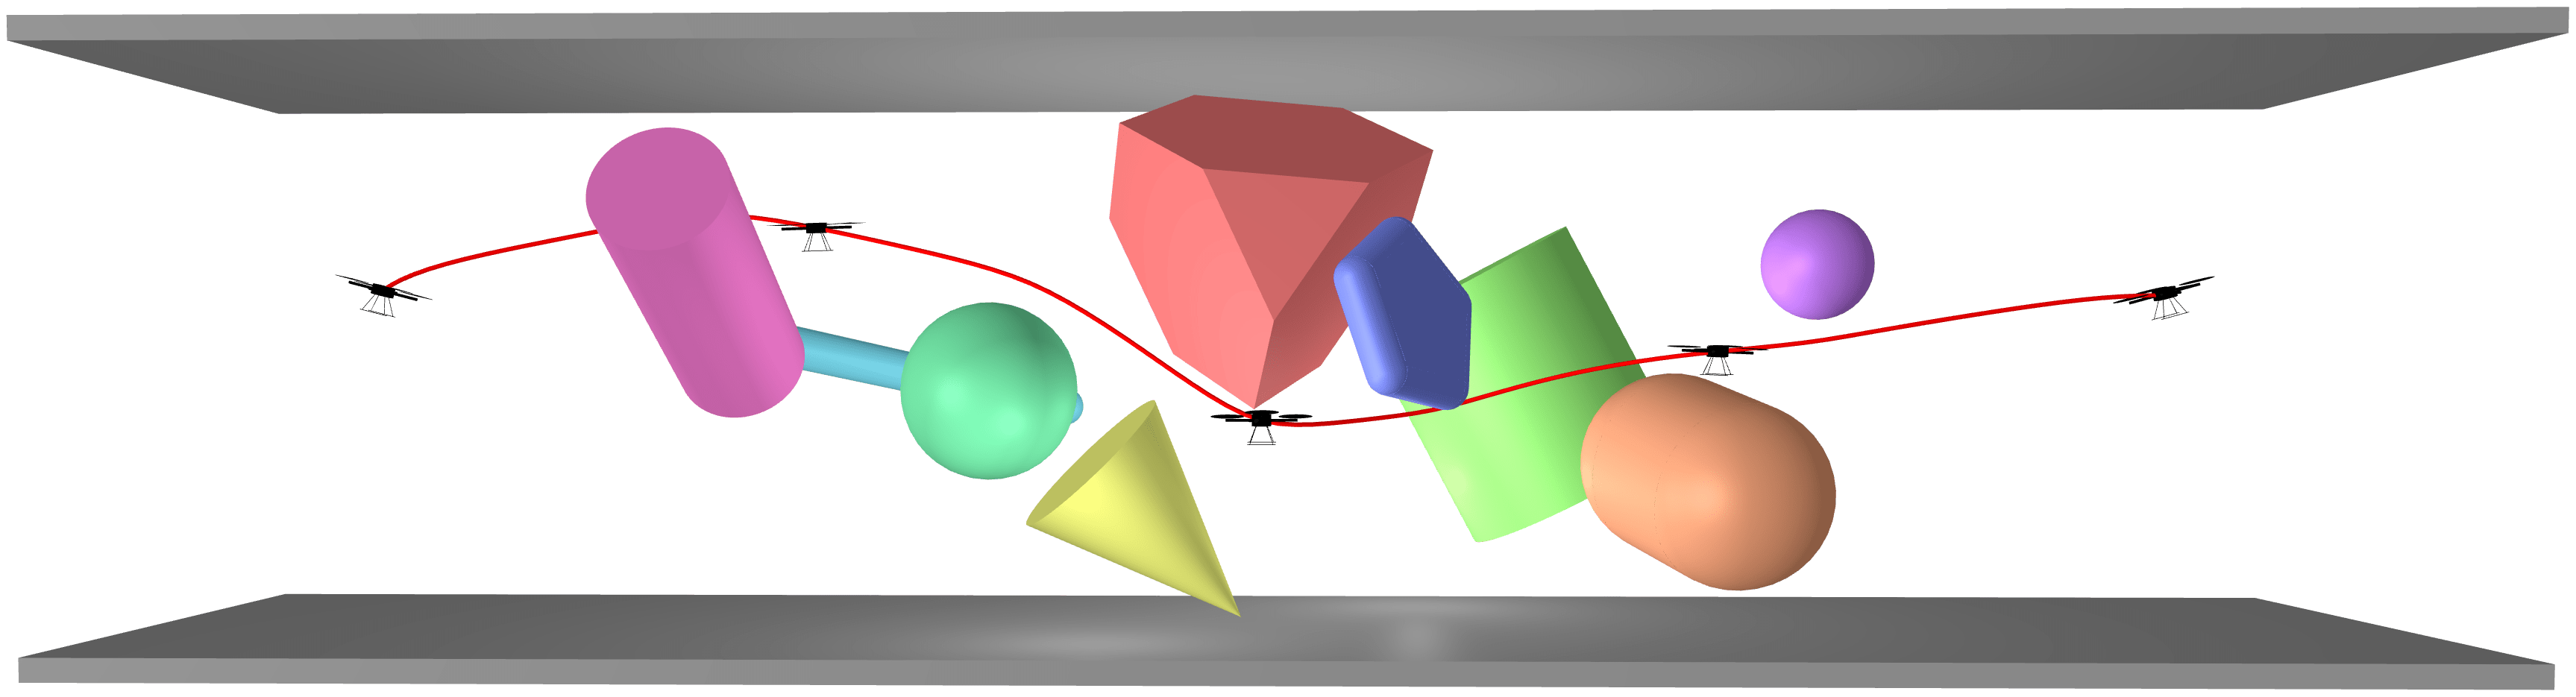
\includegraphics[width=.9\textwidth]{figures/hallway_v5.png}
%     \caption{Trajectory optimization for a 6-DOF quadrotor as it moves from left to right through a cluttered hallway. The collision constraints were represented with DCOL, and the trajectory optimizer was initialized with a static hover at the initial condition.}
%     \label{fig:hallway}
% \end{figure*}
\subsubsection{``Piano Mover'' Problem}
The first problem we will look at is a variant of the \textit{``Piano Mover''} problem, where a piano must maneuver around a 90-degree turn in a hallway \cite{wilson2013,schwartz1983}. The walls are 1 meter apart, and the ``piano'' (a line segment) is 2.6 meters long, making the path around the corner nontrivial. This problem is solved with trajectory optimization and collision constraints, where the piano is parameterized as a cylindrical rigid body in two dimensions, with a position and orientation, and the hallway is modeled with polytopes. The solution to this problem is shown in Fig. \ref{fig:piano}, where the piano successfully maneuvers around the tight corner and reaches the goal state without traveling through any of the walls. The trajectory optimizer was initialized with the piano in a static pose at the initial condition.
\cite{wilson2013} \cite{schwartz1983}
\begin{figure}[t]
\centerline{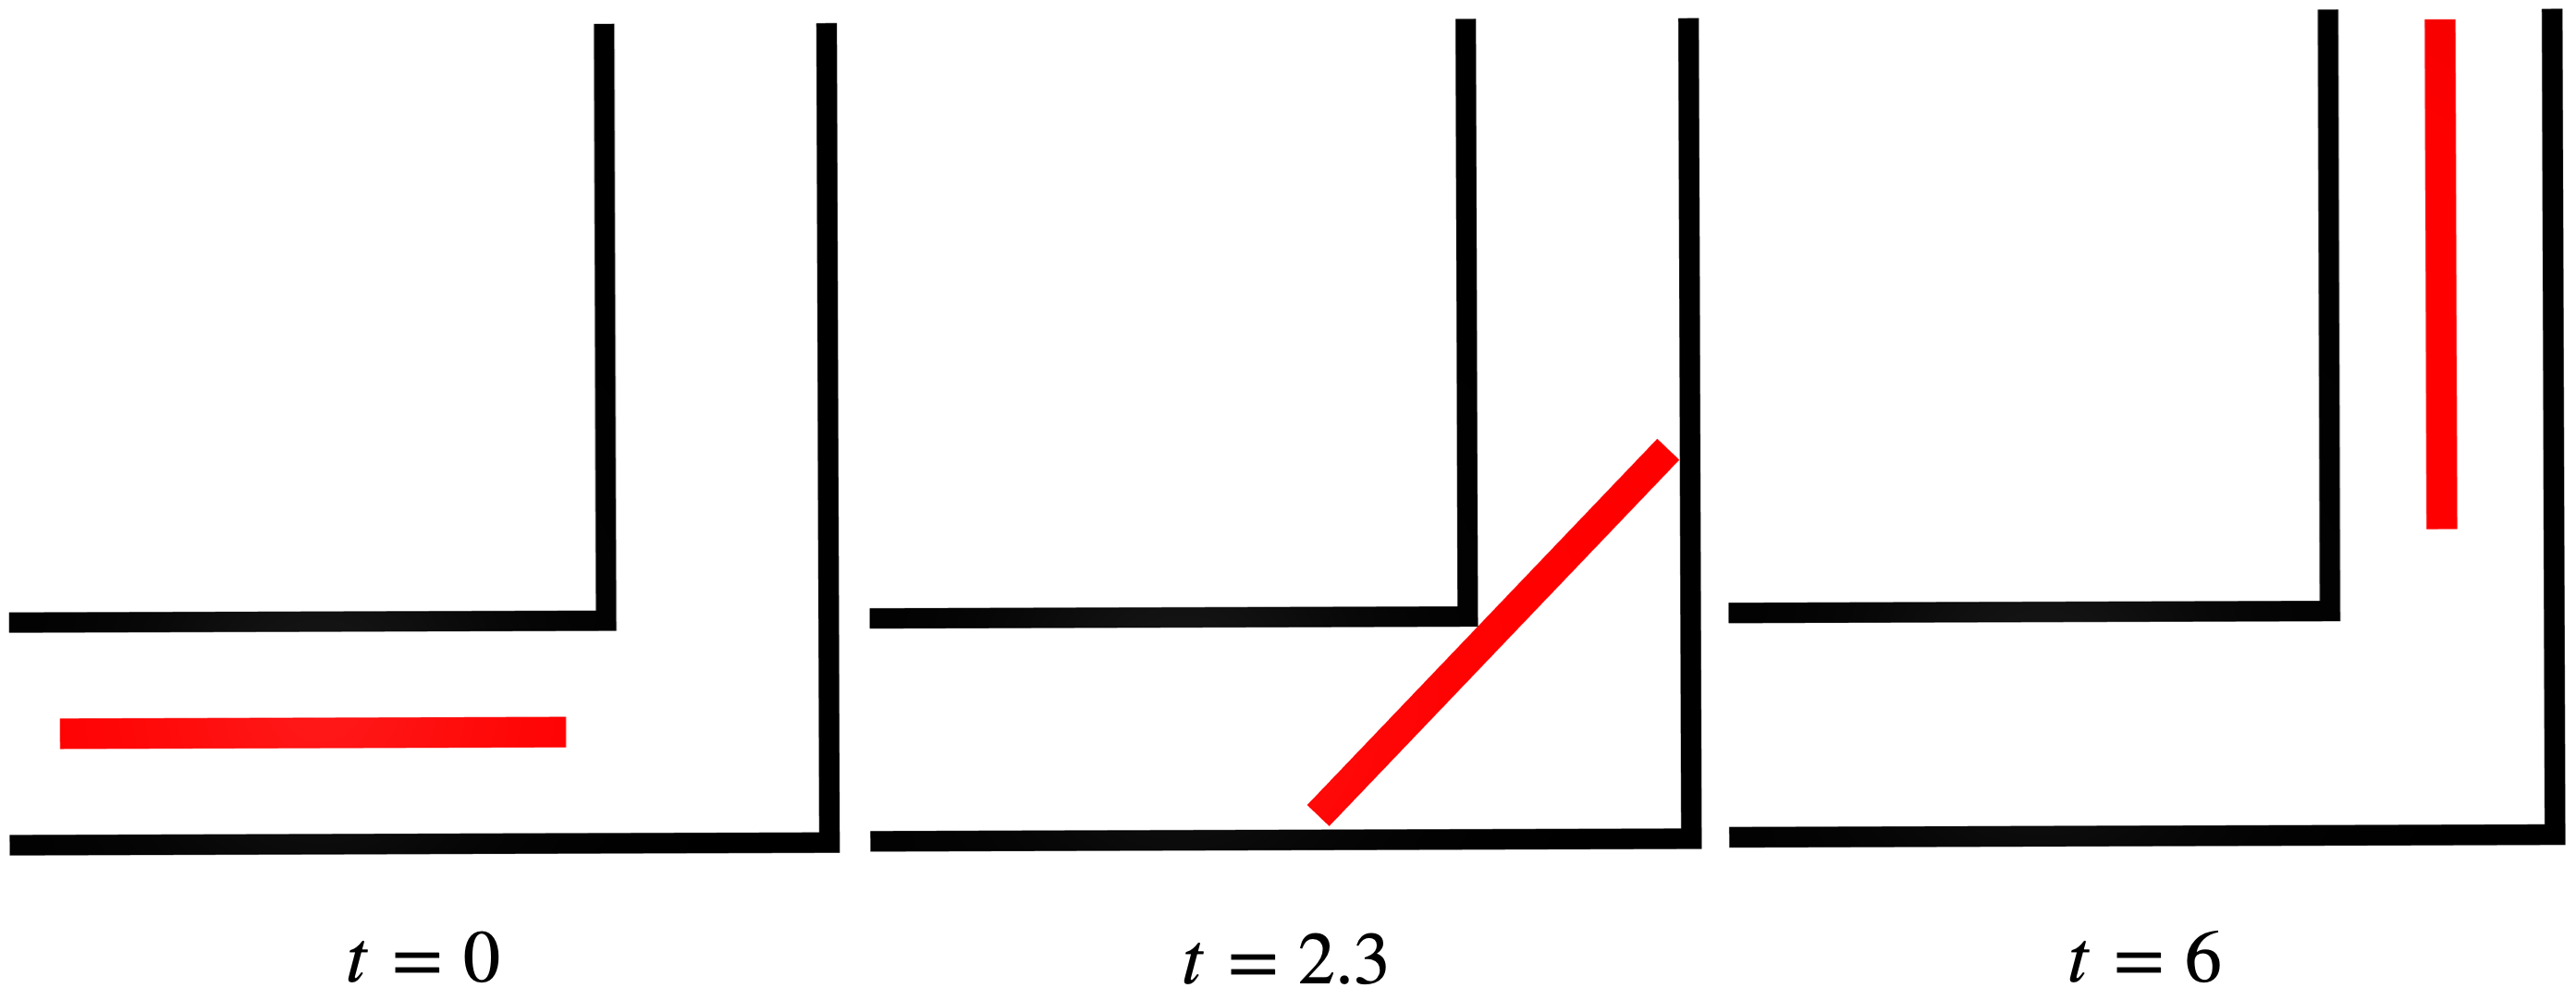
\includegraphics[width = .95\columnwidth]{figures/piano_mover_v3.png}}
\caption{The \textit{``Piano Movers"} problem, where a ``piano'' (red rectangle) has to make a turn down a hallway, is solved with trajectory optimization. The piano and the walls are modeled as rectangular prisms. DCOL was used to represent all of the collision avoidance constraints that ensure the piano cannot travel through the wall, and the trajectory optimizer was able to converge on a feasible trajectory to deliver the piano to the goal state.}
\label{fig:piano}
\vspace{-10pt}
\end{figure}
\subsubsection{Quadrotor}
Motion planning for quadrotors has received significant attention in recent years \cite{mellinger2011,mellinger,sun2022}, with collision avoidance featured in many of these works \cite{falanga2020,penicka2022,shraim2018}. With DCOL, we are able to directly and exactly incorporate collision avoidance constraints into a quadrotor motion planner to solve for trajectories through cluttered environments. In this example, we use trajectory optimization for a classic 6-DOF quadrotor model from \cite{mellinger2011,jackson2020} to solve for a trajectory that traverses a cluttered hallway with 12 objects in it, shown in Fig. \ref{fig:hallway}. The solver was initialized with the quadrotor hovering at the initial condition, and a spherical outer approximation of the quadrotor geometry was used to compute collisions. Despite this naive guess, the solver was able to quickly converge on a collision-free trajectory through the obstacles. 
% \todo{add timing?}
\subsubsection{Cone Through an Opening}
This example demonstrates how trajectory optimization with DCOL can route a cone through a square hole in a wall, as shown in Fig. \ref{fig:conewall}. The dynamics of the cone are modeled as a rigid body with full translational and rotational control, and the wall is comprised of four rectangular prisms, making a rectangular opening in the wall. The trajectory optimizer converged on a solution where the cone successfully passes through the opening in the wall, requiring that the cone slewed its orientation and ``squeezed through'' the opening.  This example demonstrates the importance of the differentiability of the collision avoidance constraints, as the optimizer was forced to leverage both translational and rotational manipulation of the cone in order to successfully pass through the opening.  As with the previous two examples, there was no expert initial guess provided to the trajectory optimizer, just a static initial condition. 
\begin{figure}
\centering
\subfloat[]{%
  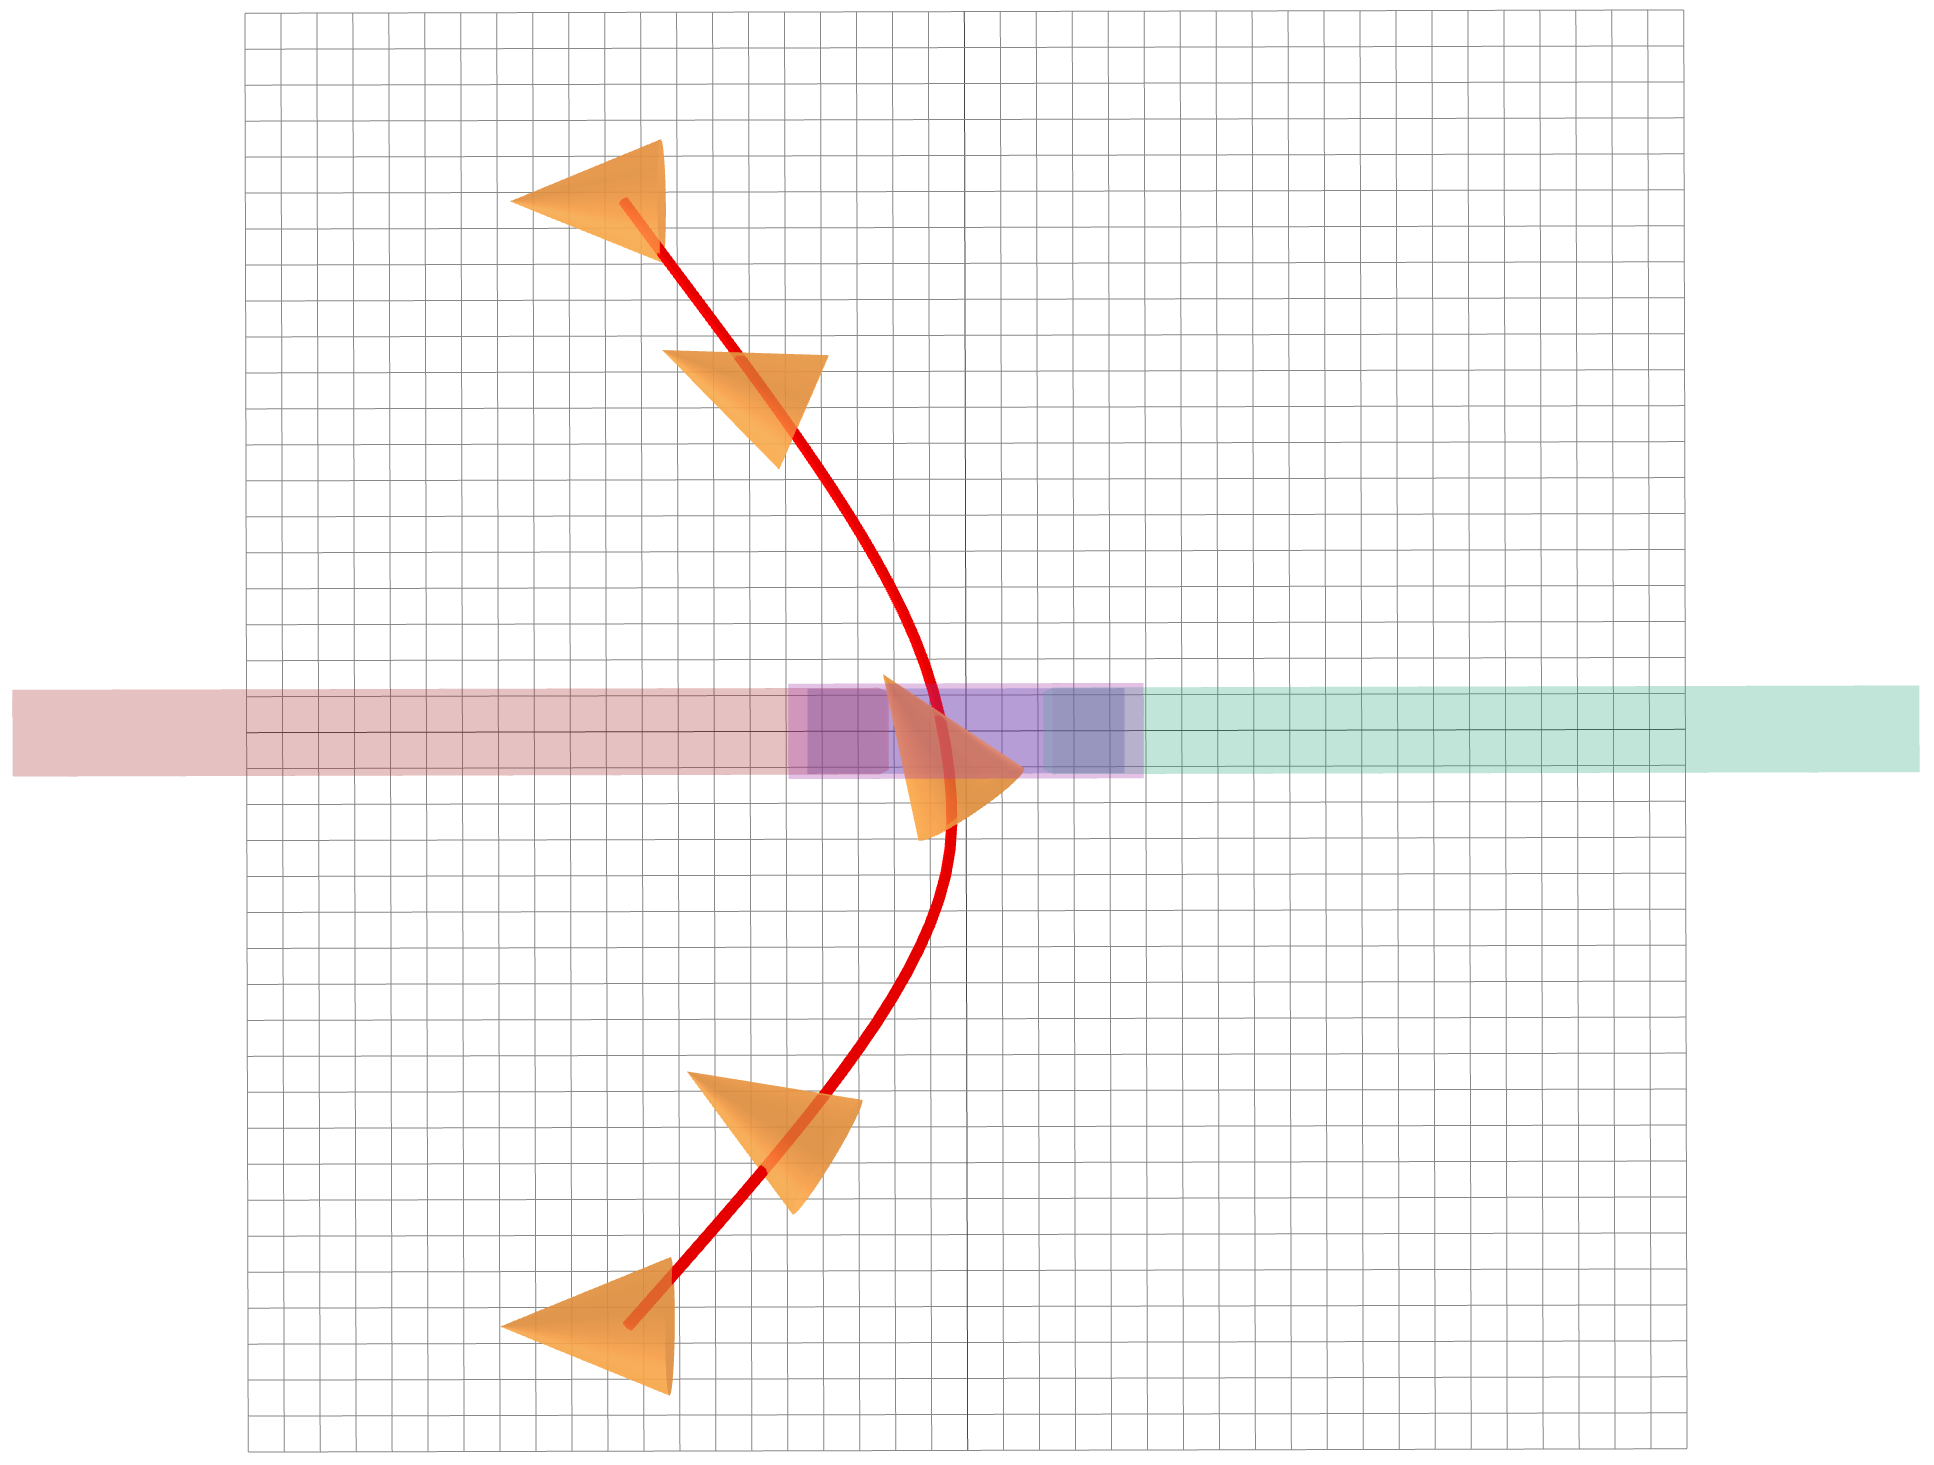
\includegraphics[clip,width=.65\columnwidth]{figures/hole_in_wall/hole_top_wire.png}%
}
 
\subfloat[]{%
  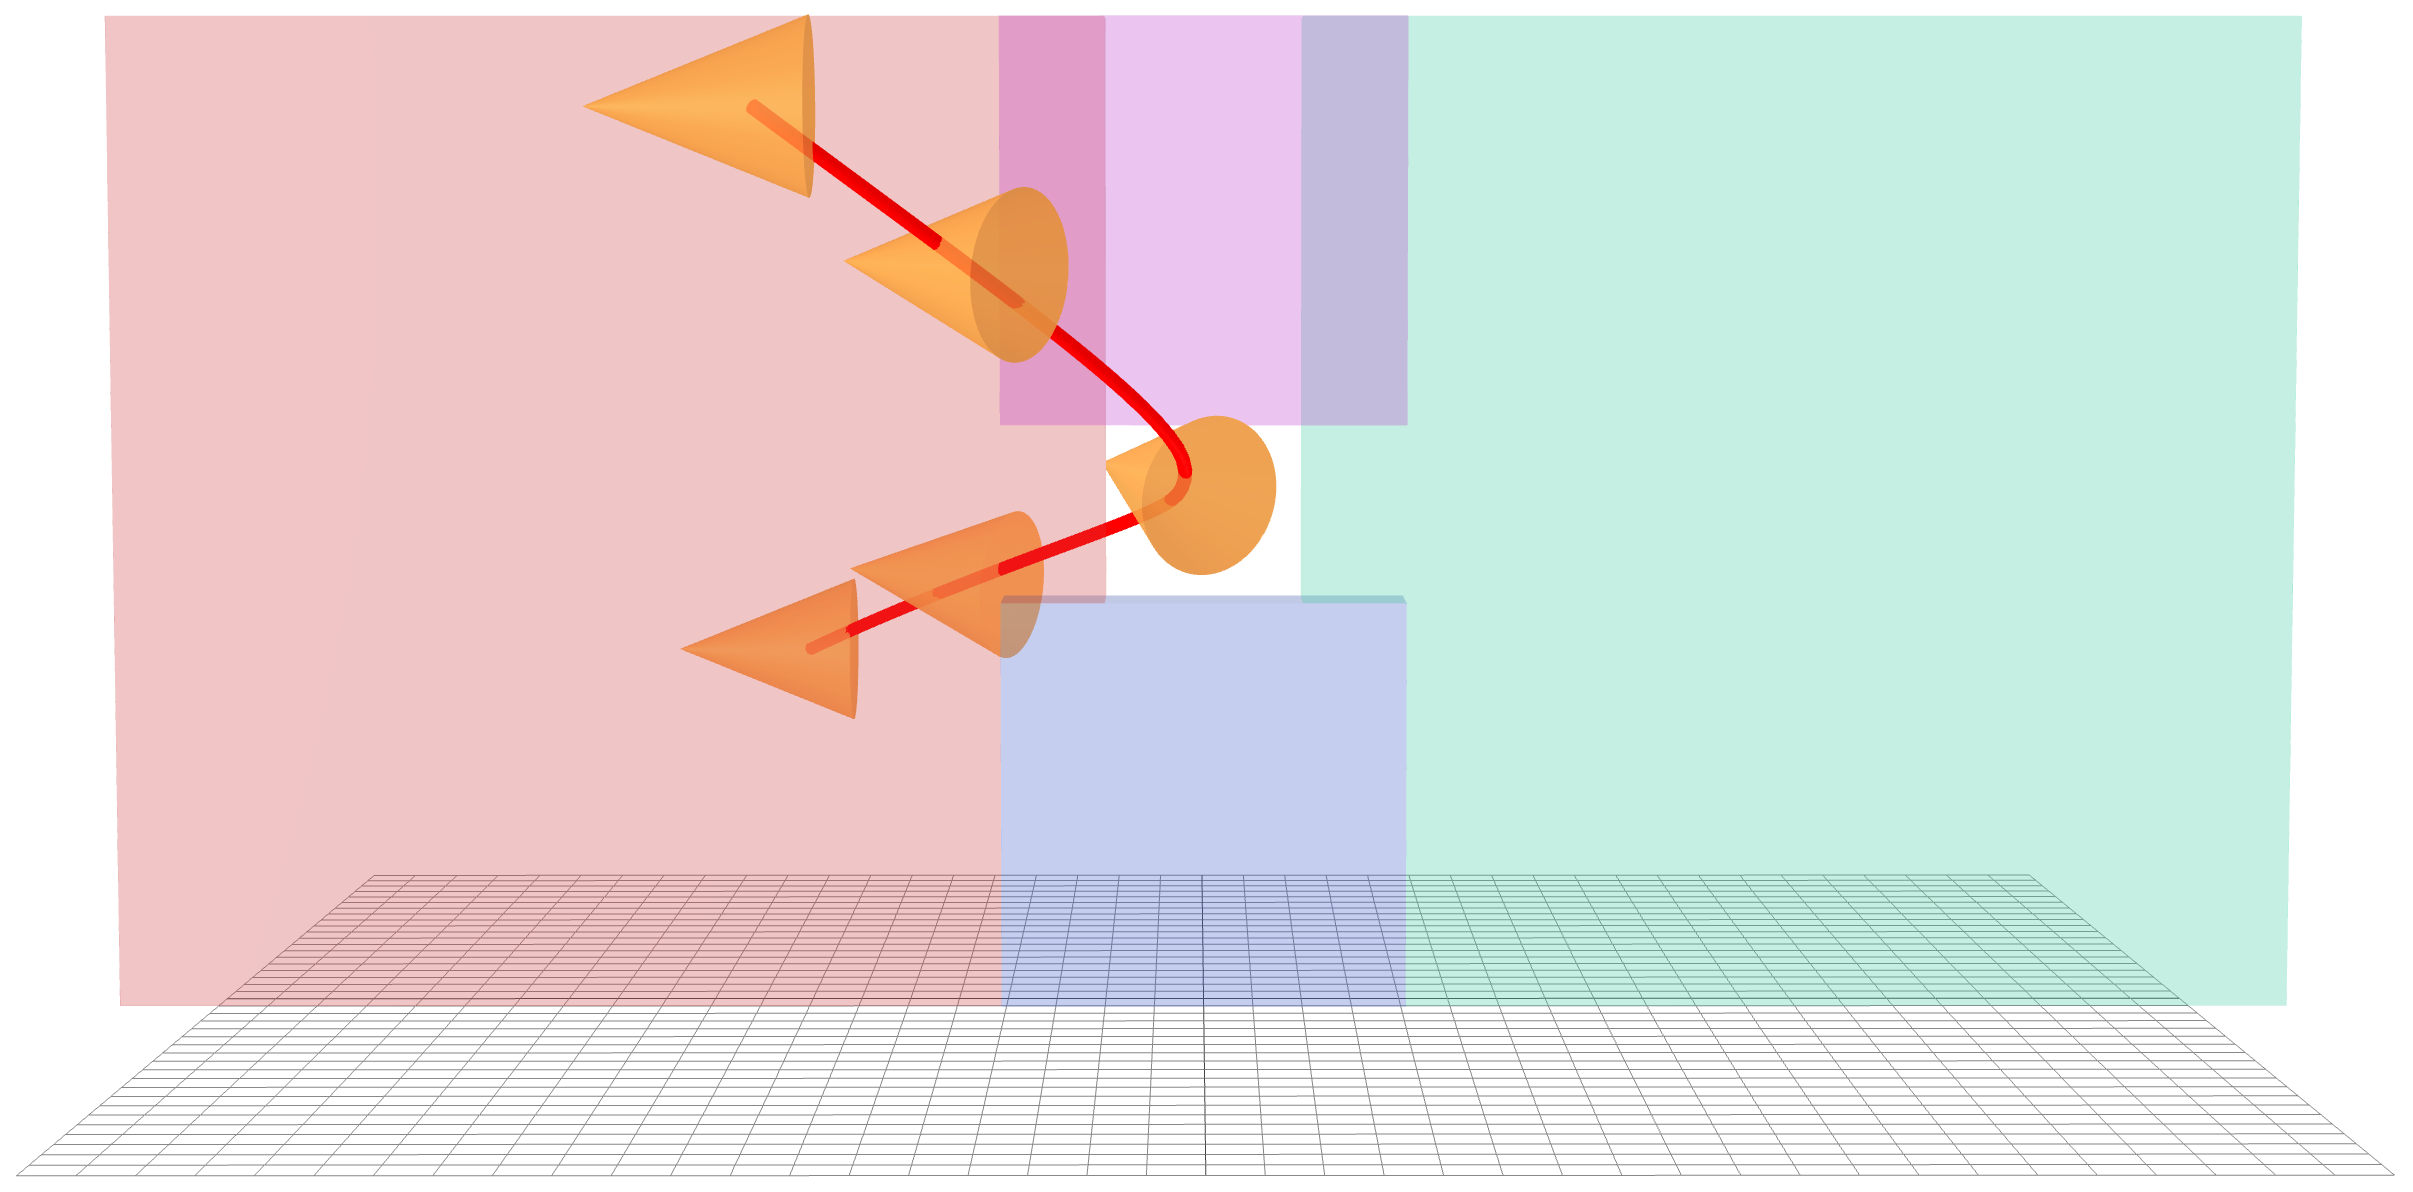
\includegraphics[clip,width=0.8\columnwidth]{figures/hole_in_wall/hole_side_wire.png}%
}
\caption{Trajectory optimization for a cone (orange) with translation and attitude control as it travels through a square opening in a wall. Top-down and side views are shown in (a) and (b), respectively. The cone is forced to slew to an attitude that allows for the passing of the cone through the opening before returning to the initial attitude. The trajectory optimizer was simply initialized with the static initial condition.}
\label{fig:conewall}
\end{figure}
\subsection{Contact Physics}
Another application of differentiable collision detection in robotics is contact physics for simulation. Rigid-body mechanics with inelastic collisions can be simulated using complementarity-based time-stepping schemes \cite{howell2022}, where stationary points of a discretized action integral are solved for subject to contact constraints \cite{marsden2001}.  Normally these constraints are limited to traditionally differentiable ones like those between fixed contact points and a floor.  The differentiability of DCOL enables these same methods to be extended for simulating contact between convex primitives, as shown in Fig. \eqref{fig:mashup} where twelve primitives collide.  In terms of computation times, using DCOL for contact physics is reasonable given each constraint evaluation and differentiation are usually less than 10 $\mu$s as shown in Table \ref{speed_table}.
% Variational integrators \cite{marsden2001} can be used to accurately simulate rigid body mechanics with inelastic collisions \cite{howell2022}, and work by finding stationary points of a discretized approximation of the action integral. This allows for the direct incorporation of differentiable collision constraints. 
% Just as with trajectory optimization, the collision constraint can be represented as $\alpha(q) \geq 1$, where $q$ are the configurations of two primitives. This means that within the variational integrator, a contact force $\rho \in \R{}$ is introduced for each collision constraint, such that the following set of complementarity constraints are satisfied:
% \begin{align}
%     \alpha(q) \geq 1,\quad  \rho \geq 0,\quad  (\alpha(q)-1) \cdot \rho =0,
% \end{align}
% where $\alpha(q) \geq 1$ ensures there is no interpenetration, the contact force $\rho$ must be positive, and $ (\alpha(q)-1) \cdot \rho =0$ guarantees that there is no contact force without collision. The incorporation of these constraints is straightforward but only if derivatives $\partial \alpha / \partial q$ are available, made possible by DCOL.
% To demonstrate the utility and robustness of this approach for contact physics, 
\begin{figure}[t]
\centerline{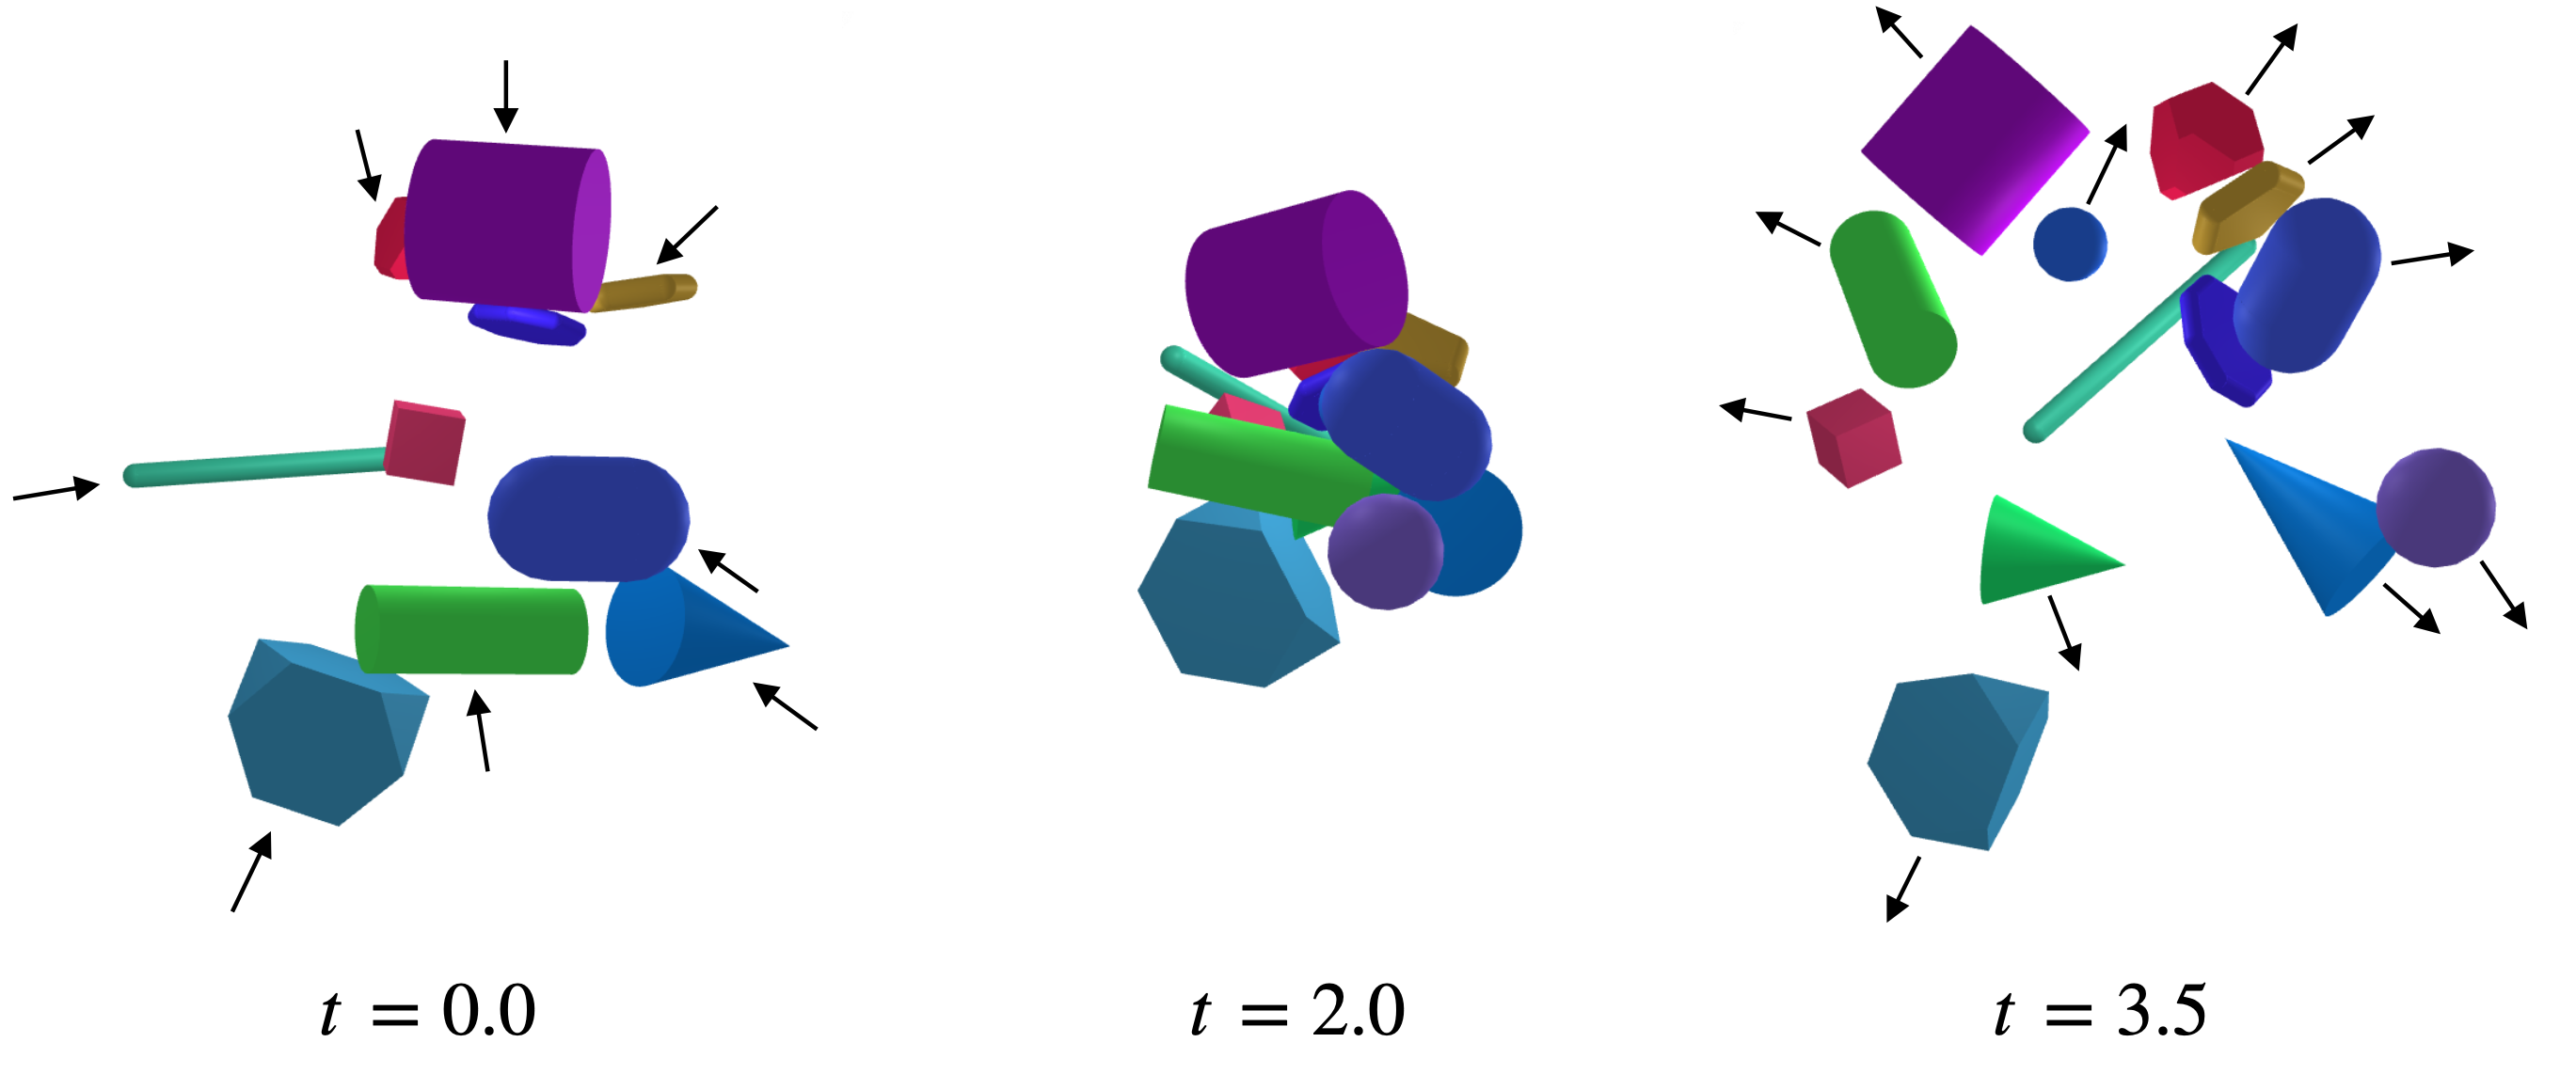
\includegraphics[width = .98\columnwidth]{figures/mashup.png}}
\caption{Contact physics with differentiable collision constraints embedded in a complementarity-based time-stepping scheme, simulated at 100 Hz.  Twelve convex objects are started at random positions with velocities pointing towards the origin at $t=0$. The objects impact each other at $t=2$ and spread out again by $t=3.5$.  Despite the complexity of the simulation, the collision constraints can be enforced to machine precision and the integration is stable.}
\label{fig:mashup}
\vspace{-10pt}
\end{figure}
\section{Conclusion}\label{sec:dcol:conclusion}
We have presented DCOL, a fast differentiable collision detection algorithm capable of computing useful collision information and derivatives for pairs of any of six convex primitives. By formulating the collision-detection problem as an optimization problem that solves for the minimum uniform scaling that must be applied to each primitive before an intersection occurs, a surrogate proximity value is returned that is informative for primitives with or without a collision. Using differentiable convex optimization and a primal-dual interior-point conic solver, smooth derivatives of this optimization problem are returned after convergence with very little additional computation. The utility of DCOL is demonstrated in a wide variety of robotics applications, including motion planning and contact physics, where collision derivatives are required. Future work includes methods for convex decompositions of complex shapes as well as the incorporation of DCOL into existing physics engines. Our open-source Julia implementation of DCOL is available at \url{https://github.com/kevin-tracy/DifferentiableCollisions.jl}. 




%%% Local Variables:
%%% coding: utf-8
%%% mode: latex
%%% TeX-engine: xetex
%%% TeX-master: "../thesis"
%%% End:
% \graphicspath{{cdcol/}}


\chapter{Differentiable Continuous Collision Detection}
\label{sec:cdcol}

Typical discrete collision detection can only consider robots and environments in their static configurations at discrete time steps. For sequences in which either the robot or the environment moves, discrete collision detection is unable to reason about collisions that occur \textit{between} time steps. This can result in accidental collisions, as well as ``tunneling,'' where two objects pass directly through one another. By contrast, continuous collision detection directly models and evaluates motion between two adjacent time steps. These continuous methods are often computationally expensive and nondifferentiable, restricting them to simple primitives for practical use in robotics. In this work, we present a method for performing continuous collision detection on arbitrary convex sets that reduces to a small convex optimization problem.  The proposed formulation is indifferent to penetration, has no degenerate cases, and is fully differentiable and highly parallelizable. Videos, code, and more examples are available at \url{https://continuous-collisions.github.io/}.

\section{Introduction}\label{sec:cdcol:introduction}
% \todo{Maybe introduce Continuous Collision Detection (CCD) and Discrete Collision Detection (DCD) everywhere?}
%
%
%
%
% Fast and accurate collision detection is a fundamental part of robotic simulation, motion planning, and control. For tasks where collisions must be avoided and tasks where collisions are a means to manipulation, collision information is a critical part of any model-based algorithm. Broadly speaking, collision information is computed on a pairwise basis and can contain closest points between objects, contact normal vectors, penetration depths, and time of contacts. 
%
Given two objects in fixed configurations, Discrete Collision Detection (DCD) is used to determine if and where a collision exists. Modern robotic motion planning tools rely on collision detection between convex objects to synthesize collision-free trajectories. When DCD is used to identify collisions in a trajectory, it runs the risk of missing unintentional collisions between the discrete time steps. These collisions come from an effect called ``tunneling,'' where an object speeds through an obstacle without violating collision avoidance constraints. This happens when collision checking is performed just before and after the object passes through the obstacle. In early video game engines, this would often result in players speeding through walls or getting stuck underneath floors \cite{ericson2004}.
%
%
\begin{figure}[t!]
\centering 
% \begin{tikzpicture}
%     \draw (0, 0) node[inner sep=0] {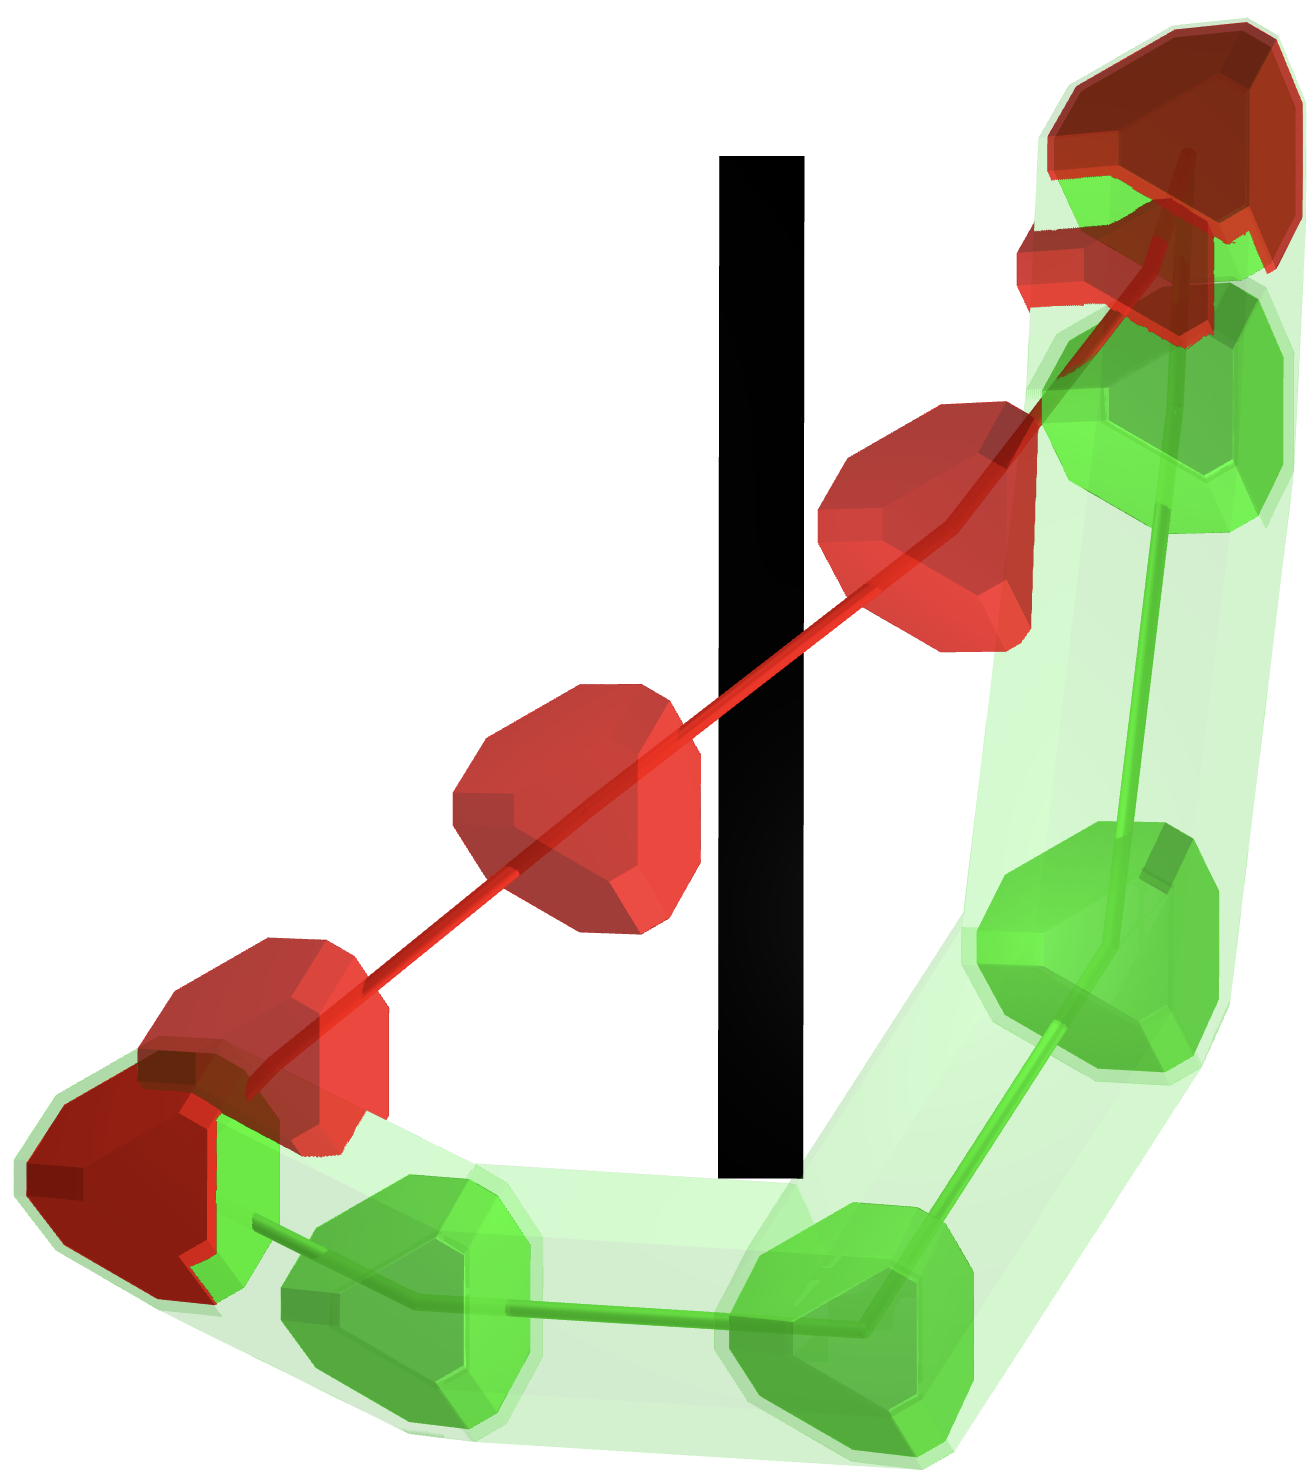
\includegraphics[width=2.4in]{figures/thru_wall/thru_wall_2.png}};
%     \node at (-3.615,3.085)[fill=red!90, text=white] {Discrete};
%     \node at (-3.4,2.4) [fill=green!90, text=black] {Continuous};
% \end{tikzpicture}
\includegraphics[width=.8\linewidth]{figures/thru_wall/thru_wall_3.png}
\caption{
Example trajectory optimization solutions for a polytope passing near a wall where collision avoidance constraints are specified with discrete collision detection (red) and the proposed continuous collision detection (green). In the discrete case, the solver only has to satisfy the collision avoidance constraints at each of the discrete knot points, allowing the polytope to ``speed'' through the wall while appearing collision-free to the solver. Using the proposed continuous collision detection, the solver is able to directly reason about collision that happen at and between the time steps to ensure that no collision exists.
}
\label{fig:thru_wall}
\end{figure}

To ensure that DCD is adequate for collision avoidance planning, a myriad of algorithmic enhancements have been proposed to combat these shortcomings. First, the time between discrete collision checks can be decreased, resulting in finer-grained collision checking at the expense of compute and problem complexity. Another common strategy is to add a collision margin that is conservative enough to combat any tunneling by making obstacles appear thicker than they are. In cuRobo~\cite{sundaralingam2023}, this collision margin is augmented with a penalty that effectively increases the margin when the robot is moving faster, thus discouraging any ``speeding through'' obstacles. In TrajOpt~\cite{schulman2013a}, collisions between pairs of convex objects at adjacent time steps are avoided by forming a convex hull for each object and checking these convex hulls for any intersections. This approach successfully captures continuous collisions but is a potentially limiting over approximation of the collision environment since the objects are not actually encompassing the convex hulls for the duration of the time step. 

Based on the complexity of the primitive, there are many available methods for DCD that each carry their own tradeoffs. For simple sphere-capsule-box interactions, analytical collision information can be solved for in closed form \cite{ericson2004}. For generic convex shapes, iterative methods such as Gilbert-Johnson-Keerthi (GJK) \cite{gilbert1988, cameron1997} and Minkowski Portal Refinement (MPR) \cite{snethen2008,newth2013} are used. Both GJK and MPR only return useful collision information when objects are not in contact; as soon as penetration occurs, the Expanding Polytope Algorithm (EPA) \cite{vandenbergen2001} must be used to determine a penetration depth. Highly mature implementations of these algorithms are available in the Flexible Collision Library (FCL) \cite{pan2012}, which many modern physics simulators rely on \cite{coumans2015,tedrake2019a,lee2018,todorov2012a}.  While these DCD algorithms are fast and reliable, they involve significant logic and branching, making them inherently nondifferentiable and challenging to put on a GPU. 
%
%

While DCD examines pairs of objects in static configurations, Continuous Collision Detection (CCD) reasons about objects as they move between sequential configurations. CCD computes the same information that DCD does, but in addition, also calculates the time of impact, indicating when a collision takes place between two configurations. This new information comes at an expense, as CCD is significantly more difficult and limited in the primitives it can handle compared to DCD. For simple sphere-capsule-box primitives, a mix of analytical and iterative methods are available for computing the time of impact~\cite{ericson2004}. In \cite{vandenbergen2004}, a GJK-based ray-casting method was proposed to compute the continuous collision information between a moving convex object and a static configuration-space obstacle. A method for direct handling of moving nonconvex meshes was introduced in \cite{zhang2006}, and was updated to include angular motion in \cite{coumans}. While these existing CCD methods are readily available, they suffer from the same branching and nondifferentiability issues as DCD methods.

This work focuses on convex-convex CCD as it relates to gradient-based motion planning, where cost and constraint functions are required to be differentiable. There has been growing interest in differentiable DCD with sampling-based methods \cite{montaut2022a}, and differentiable optimization-based methods \cite{tracy2023b,zimmermann2022,tracy2022}.  The work proposed in this paper serves more closely as a continuous follow-on to the differentiable DCD solution introduced in \cite{tracy2023b}, where a framework for computing smooth gradients through collision detection was enabled by scale-based collision detection and differentiable convex optimization. 

We introduce a true CCD routine for pairs of arbitrary convex sets that is fully differentiable with respect to each configuration. By solving for collision information with a geometric scale factor, the collision check reduces to a small convex optimization problem that is guaranteed to be globally solvable, bounded, and feasible for any configuration of the objects.  The solution of this optimization problem is then used to form smooth gradients of the collision information with respect to any problem parameters with very limited computational expense (significantly less than solving the problem). Together, this enables gradient-based motion planners to solve for collision-free trajectories with a coarse and efficient discretization of the trajectories.

Our specific contributions in this paper are the following:
\begin{itemize}
    \item An optimization-based continuous collision-detection method between pairs of moving convex sets without any branching or degenerate cases 
    \item A fast and efficient method for differentiating the method in automatic-differentiation frameworks
    \item A convex interior-point algorithm for solving the collision problem that can be arbitrarily parallelized on a GPUs or TPUs for problems with varying numbers of constraints
\end{itemize}

This paper proceeds by providing background information in Section \ref{sec:cdcol:background}, introducing our CCD algorithm in Section \ref{sec:cdcol:cdcol}, detailing a parallelizable convex solver in Section \ref{sec:cdcol:qp_solver}, examples of these methods used for collision avoidance motion planning in Section \ref{sec:cdcol:examples}, and our concluding remarks in Section \ref{sec:cdcol:conclusion}.
%
%
% \begin{figure}[t!]
%     \centering
%     \includegraphics[width=.47\textwidth]{figures/ballet/ballet1.png}
%     \caption{A multi-robot assembly task where four robotic arms interact with a structure in a common workspace. The proposed continuous collision detection is used to certify trajectories as collision-free and is fully differentiable with respect to the configurations of the robots.}
%     \label{fig:growth}
% \end{figure}
%
%
\section{Background}\label{sec:cdcol:background}
%
%
%
%
The continuous collision-detection algorithm introduced in this paper involves forming, solving, and differentiating a convex optimization problem. In this section, the necessary background to understand this formulation is presented.

%
%
\subsection{Perspective Operators} \label{sec:cdcol:perspective}
% %
% %
% \begin{figure}[]
%     \centering
%     \includegraphics[width=.4\textwidth]{figures/growth/growth.png}
%     \caption{Demonstration of the scaling factor $\alpha$ as applied to a convex set. The original set, shown when $\alpha = 1$, is uniformly scaled down for $\alpha < 1$ and and up for $\alpha > 1$. As $\alpha \rightarrow 0$ the set becomes just a single point. This scaling idea is formalized as a perspective operator, where an arbitrary convex set can be scaled up and down in this fashion.}
%     \label{fig:growth}
% \end{figure}
% %
% %
In order to simplify the notation around scale-based collision detection, the idea of a perspective operator for a convex set is introduced. For collision purposes, each rigid body in a robot is decomposed into a collection of convex sets \cite{schulman2013a}.
Given a closed convex set $\mathcal{X} \subseteq \mathbf{R}^N$, a perspective operator is used to map this $n$-dimensional set to a cone in $n+1$ dimensions \cite{marcucci2023, marcucci, rockafellar1997, hiriart-urruty1993}.
The new dimension comes from a scale factor $\alpha \in \mathbf{R}_+$ that geometrically scales up the set when $\alpha > 1$ and scales down the set when $\alpha \leq 1$ until it is just a point at $\alpha = 0$. 
% This scaling and its effect on a convex set are demonstrated in Fig. \ref{fig:growth}. 

For practical purposes, the simplest way to exploit the perspective operator is to define the original convex set in standard conic form, $\mathcal{X} = \{x : Ax + b \in \mathcal{K}\}$, where $x \in \R{3}$ is a point in some world frame $\mathbb{W}$, and $\mathcal{K}$ is a proper convex cone \cite{boyd2004, lobo1998}. Common convex sets such as polytopes, cylinders, cones, capsules, and ellipsoids, can easily be represented in this form \cite{tracy2023b}. From here, the perspective operator defines a new scaled convex set $\bar{\mathcal{X}}$ as the following:
%
\begin{align}
    \bar{\mathcal{X}} &= \{(x, \alpha) : \alpha \geq 0, Ax + \alpha b \in \mathcal{K}\}.
\end{align}
%
For example, for a polytope described by $Bx + c \geq 0$ (where the cone $\mathcal{K}$ is the nonnegative orthant $\mathbf{R}_+$), the scaled polytope becomes $Bx + \alpha c \geq 0$.

It is often most convenient to express a convex set with an attached body frame $\mathbb{B}$, with an origin $\mathbb{B}_0$. Instead of redefining the convex set every time it moves in the world frame, we can instead simply define it once in its own body frame and parameterize any SE(3) rigid transformation with translation $r = {}^\mathbb{W} r {}^{\mathbb{B}_0}_\mathbb{B} \in \R{3}$ and rotation $Q = {}^\mathbb{W} Q {}^\mathbb{B} \in \R{3 \times 3}$. This allows us to write a general constraint for a convex set given a specific position and attitude as:
%
\begin{align}
    A Q^T(x - r) + \alpha b &\in \mathcal{K}. \label{eq:se3_standard_form}
\end{align}
%
This method for defining scaled convex sets in a world frame enables a straightforward extension to optimization-based collision detection built on this scaling. 
%
%
\subsection{Scale-Based Collision Detection}\label{sec:cdcol:background_scale_based}
%
%
\begin{figure}
\centering
\begin{tabular}{p{.6cm}cc}
\toprule
   &
  initial configuration & scaled to collision 
  \\
  \midrule
  \begin{tabular}{l}
    \small with \\
    \small collision
  \end{tabular} &
  \begin{tabular}{l}
   \includegraphics[height=1.5cm]{figures/four_panel/one.png}
  \end{tabular} & \begin{tabular}{l}
   \includegraphics[height=1.5cm]{figures/four_panel/two.png}
  \end{tabular}\\
  % \hline
  \begin{tabular}{l}
    \small without \\
    \small collision
  \end{tabular} &
  \begin{tabular}{l}
    \begin{tabular}{l}
   \includegraphics[height=1.1cm]{figures/four_panel/three.png}
  \end{tabular}
  \end{tabular} & \begin{tabular}{l}
   \includegraphics[height=1.1cm]{figures/four_panel/four.png} \end{tabular}\\
% \hline
\bottomrule
\end{tabular}
\caption{Scale-based collision detection for objects that are in and out of collision. In the upper row, the two objects are not in collision, so the minimum scaling that results in an intersection is able to ``grow'' the objects to $\alpha^* = 1.3$. In the bottom row, the two objects are already in collision, so the minimum uniform scaling shrinks the objects down to $\alpha^* = 0.8$.}
\end{figure}
%
%
Traditionally, collision detection between two convex sets is done by searching for the closest point between these two sets. If the closest points are not coincident, the objects are not in collision. This is the backing for the popular collision detection algorithms GJK~\cite{gilbert1988, cameron1997} and MPR~\cite{snethen2008,newth2013}, enabling fast and efficient collision detection between common convex primitives. The two main drawbacks of this approach come from nondifferentiability of these algorithms and the degenerate case when the two sets are in collision. In the latter case, GJK and MPR cannot return useful information and instead must default to an alternative algorithm such as EPA to establish a ``penetration depth.'' 

As shown in \cite{tracy2023b}, scale-based collision detection avoids both of these shortcomings by solving a different optimization problem. Instead of searching for the closest points between two fixed sets, the perspective operator is used to scale the two sets by a common $\alpha$ and solve for the minimum shared scaling that results in an intersection. 

With a point in the world frame $x \in \R{3}$ and two convex sets defined with \eqref{eq:se3_standard_form} as $A_iQ_i^T(x - r_i) + \alpha b_i \in \mathcal{K}$, the optimization problem that finds the minimum scaling $\alpha$ that results in an intersection between two scaled convex sets is:
%
\begin{mini}
{x, \alpha}{ \alpha}{\label{dcol2}}{}
% \addConstraint{A_1 Q_1^T(x - r_1) + \alpha b_1}{\in \mathcal{K}_1}{}
% \addConstraint{A_2 Q_2^T(x - r_2) + \alpha b_2}{\in \mathcal{K}_2}{}
\addConstraint{A_i Q_i^T(x - r_i) + \alpha b_i}{\in \mathcal{K}_i}{\quad i = 1, 2}
\addConstraint{\alpha}{\geq 0.}{}
\end{mini}
%
This is a convex optimization problem that is guaranteed to be both feasible and bounded. In the event that the two convex sets are in collision, the sets are scaled down to $\alpha < 1$ to the smallest possible scale factor that has an intersection. If the two sets are not in collision, they are scaled up to $\alpha > 1$ until an intersection is reached. In both cases, the fundamental algorithm remains unchanged, as the optimization formulation in ~\eqref{dcol2} handles both cases. Furthermore, there are no degenerate cases based on the geometry or configurations of the sets, since there always exists a minimum scaling for an intersection, even when the intersection is another set (a line or a plane). 
%
%
\subsection{Differentiable Optimization}
%
%
Collision detection as a solution to an optimization problem in \eqref{dcol2} makes taking derivatives with automatic differentiation tools challenging. Both forward and reverse-mode automatic differentiation are unable to accurately compute derivatives through an iterative numerical solver \cite{amos2017}. To avoid this, differentiable optimization tools are used to compute these derivatives in a fast and accurate way without propagating derivatives through iterative schemes.

Given a generic optimization problem in the following form:
%
\begin{mini}
{y}{ f_\theta(y)}{\label{generic_opt}}{}
\addConstraint{c_\theta(y)}{\in \mathcal{K},}{}
\end{mini}
%
with the cost and constraints as functions of some problem parameters $\theta$, a dual variable $\lambda \in \R{m}$ is used to enforce the constraint in the following Lagrangian:
%
\begin{align}
    \mathcal{L}_\theta(y, \lambda) &= f_\theta(y) + \lambda^Tc_\theta(y).
\end{align}
%
Using this, the KKT conditions necessary for optimality are,
%
\begin{align}
    \nabla_y f_\theta(y) + \bigg[ \frac{\partial c}{\partial y} \bigg]^T\lambda  &= 0 \label{kkt:1} \\ 
    c_\theta(y) &\in \mathcal{K}\label{kkt:2} \\ 
    \lambda &\in \mathcal{K}^* \label{kkt:3}\\ 
    c_\theta(y) \circ \lambda &= 0,\label{kkt:4}
\end{align}
%
where $\mathcal{K}$ is a proper cone and $\mathcal{K}^*$ and $\circ$ are the corresponding dual cone and cone product, respectively \cite{vandenberghe}. Any primal-dual values $(y, \lambda)$ that satisfy equations \eqref{kkt:1}-\eqref{kkt:4} are a locally optimal solution to \ref{generic_opt}.

By viewing equations \eqref{kkt:1} and \eqref{kkt:4} as the following implicit function of $w = (y, \lambda)$,
%
\begin{align}
    g_\theta(w) &= \begin{bmatrix}
        \nabla_y f_\theta(y) + \big[ \frac{\partial c}{\partial y} \big]^T\lambda \\ 
         c_\theta(y) \circ \lambda
    \end{bmatrix},
\end{align}
%
an approximate primal-dual solution $w^* = (y^*, \lambda^*)$ is an equilibrium point where $g_\theta(w^*) \approx 0$. At this equilibrium, the implicit function theorem can be used to calculate the Jacobian of the primal-dual solution with respect to the to the problem parameters \cite{howell2022}:
%
\begin{align}
    \frac{\partial y}{\partial \theta} = - \bigg( \frac{\partial g}{\partial y} \bigg)^{-1}\frac{\partial g}{\partial \theta}. \label{eq:ift2}
\end{align}
%
Practically, this works by solving the problem with a standard numerical solver, after which the approximate solution is used with the implicit function theorem to provide the necessary derivatives.

Alternatively, if the only derivative we need is that of the optimal objective value $f(x^*)$ with respect to the problem parameters, an even simpler approach can be used: At a primal-dual solution, the gradient of the objective value with respect to the problem parameters is simply the gradient of the Lagrangian with respect to these same parameters \cite{castillo2006},
%
\begin{align}
    \nabla_\theta f_\theta(y^*)= \nabla_\theta \mathcal{L}_\theta(y^*, \lambda^*), \label{eq:lag_grad}
\end{align}
%
allowing us to calculate the derivative we need without forming or solving a linear system.

These differentiable optimization methods are used to convert the always-feasible convex optimization problem in \eqref{dcol2} into a fully differentiable algorithm, as shown in \cite{tracy2023b}. The optimal objective value ($\alpha$) or the primal and dual variables can be differentiated with respect to both the configurations of the objects and the geometry of the objects themselves. In \cite{tracy2023b} this was used in trajectory optimization to solve for collision-free trajectories simply by enforcing $\alpha > 1$ as a differentiable constraint in a motion planner.
%
%
%
%
\section{Continuous Collision Detection}\label{sec:cdcol:cdcol}
%
%
%
%
\begin{figure*}[t!]
    \centering
    \includegraphics[width=.8\textwidth]{figures/tau/third.png}
    \caption{Graphical description of how the $\tau \in [0, 1]$ parameter linearly interpolates the origin of the objects from their initial positions at $r_i^{(-)}$ at $\tau = 0$, to $r_i^{(+)}$ at $\tau = 1$. Discrete collision detection can only check objects for collisions at $\tau = 0$ and $\tau = 1$, while the proposed continuous collision detection method can determine whether there is a collision as each object moves between the two positions. It is important to note that this sweeping motion is \textit{not} simply checking if two convex hulls are in collision, but rather checks for contact as both objects move simultaneously on the path.}
    \label{fig:sweep_tau}
\end{figure*}
%
With the necessary background on perspective operators, scale-based collision detection, and differentiable optimization, the novel CCD algorithm can now be introduced that checks for collisions between two convex sets as they move between configurations. 

The core assumption in this CCD framework is that the two objects move linearly between time steps with a fixed attitude. This motion can be seen in Fig. \ref{fig:sweep_tau}, where two shapes ``sweep'' between the time steps. Given the two convex sets with positions $r_i \in \R{3}$ and attitudes $Q_i \in \R{3 \times 3}$, as described in Section \ref{sec:cdcol:perspective}, we can introduce the notation for time. Positions and attitudes from the first time step will be denoted with
$\Box^{(-)}$, and those from the second time step with $\Box^{(+)}$. A new normalized time parameter $\tau \in [0,1]$ is introduced where $\tau=0$ denotes the first time step and $\tau = 1$ denotes the second. Together, we can express this notation as $r_i(\tau=0) = r_i^{(-)}$, and $r_i(\tau=1) = r_i^{(+)}$. A line segment between these two positions can be calculated with the following,
%
\begin{align}
    r_i(\tau) = \tau r_i^{(-)} + (1 - \tau)r_i^{(+)},
\end{align}
%
where we simply linearly interpolate from the position at one time step to the position at the next with a constant linear velocity.  The attitudes between the time steps are simply averaged as $Q_i$, which is straightforward depending on the parameterization of the attitude~\cite{markley2014, markley2007}. Now, a scale-based collision-detection problem, similar to \eqref{dcol2}, is introduced as follows,
%
\begin{mini}
{x, \alpha, \tau}{ \alpha}{\label{cdcol}}{}
\addConstraint{A_i Q_i^T(x - \tilde{r}_i) + \alpha b_i}{\in \mathcal{K}_i,}{ \quad i = 1,2}
\addConstraint{\tau r_i^{(-)} + (1 - \tau)r_i^{(+)}}{= \tilde{r}_i,}{\quad i = 1,2}
\addConstraint{0 \leq \tau }{\leq 1}{}
\addConstraint{\alpha}{\geq 0,}{}
\end{mini}
%
where we are searching for the minimum positive scale factor $\alpha$ such that an intersection exists between the two scaled convex sets as they sweep between the time steps.  Similar to \eqref{dcol2}, a collision exists if and only if $\alpha^* \leq 1$. This is a small convex optimization problem that is guaranteed to have a solution no matter the configuration of the objects. It makes no difference to the algorithm if the objects are in or out of collision for any amount of the sweep, or if they don't collide at all. The constraint $\alpha \geq 0$ is written here as a formality, since it is implicitly satisfied by the perspective operator.

Once this problem is formed and solved, the primal and dual variables can be used to calculate the gradients of the optimal $\alpha^*$ with respect to the poses or geometries of the objects using \eqref{eq:lag_grad}. If Jacobians of the primal or dual variables with respect to the problem parameters are needed, the implicit function theorem can be used to form these derivatives with \eqref{eq:ift2}. 

For numerical stability, it is often advantageous to add a very small regularization term to \eqref{cdcol},
%
\begin{align}
    J_{{reg}} &= \epsilon [\|x - r_{avg}\|_2^2 + (\alpha - 1)^2 + (\tau - 0.5)^2 ],
\end{align}
%
where $\epsilon << 1$ and $r_{avg} \in \R{3}$ is the average of the four positions (two objects at two time steps). This regularizer serves to guarantee that \eqref{cdcol} is \textit{strongly} convex, and can sometimes help the solver converge in fewer iterations \cite{boyd2004,nocedal2006}. With a small regularizer in the range $\epsilon \in [10^{-8}, 10^{-5}]$, the regularized optimal objective value does not differ meaningfully from $\alpha^*$.
%
%
% \subsection{Time of Collision Formulation}
% %
% %
% \todo{I may remove this section}
% If a collision has been identified with \eqref{cdcol}, it may be of interest when the Time of Collision (TOC) is. This can also be solved in an optimization-based way with a very similar formulation. Instead of minimizing the scaling that results in an intersection, we can fix $\alpha = 1$ and solve for the minimum $\tau$ that results in a collision:
% %
% \begin{mini}
% {x, \tau}{ \tau}{\label{toc}}{}
% \addConstraint{A_i Q_i^T(x - \tilde{r}_i) + b_i}{\in \mathcal{K}_i,}{ \quad i = 1,2}
% \addConstraint{\tau r_i^{(-)} + (1 - \tau)r_i^{(+)}}{= \tilde{r}_i,}{\quad i = 1,2}
% \addConstraint{0 \leq \tau }{\leq 1.}{}
% \end{mini}
% %
% This problem is again a small convex optimization problem that can be solved and differentiated quickly. Unlike \eqref{cdcol}, this problem will not have a feasible solution if there is no collision, so it should only be solved if \eqref{cdcol} has already identified a collision.
%
%
%
%
\section{Parallelizable QP Solver}\label{sec:cdcol:qp_solver}
%
%
%
%
In this section, a fast and efficient Primal-Dual Interior-Point (PDIP) solver will be described that is capable of running in parallel on accelerator units (GPU/TPU). Since the optimization problem in \eqref{cdcol} is small (5 primal variables), state-of-the-art PDIP methods can solve this problem quickly and reliably. We focus on polytopes as our convex primitive, as they are expressive and result in \eqref{cdcol} being a convex Quadratic Program (QP).  

Writing convex optimization solvers on a GPU has become significantly easier in recent years, with the advent of domain-specific languages like PyTorch \cite{paszke2019} and JAX \cite{bradbury2018}. High-level Python code can be compiled to run directly on GPUs/TPUs allowing for massively parallel computation with minimal implementation effort. 

The challenge in scaling up these computations for our proposed collision detection comes from the varying sizes of the convex sets in the scene. Since we are focusing on polytopes in this section, this translates to dealing with polytopes with different numbers of faces. In JAX, the best way to parallelize a computation is to call the same function over a list of equal sized arrays. In the case of polytopes with varying numbers of faces, this results in QPs with different numbers of constraints, violating our assumption of equal-sized arrays. 

In order to ensure that the arrays being parallelized over are of equal size, many algorithms simply choose the largest array in the set and pad all of the smaller arrays with zeros. In the case of constraints for a QP solver, this results in redundant constraints, violating the Linear Independence Constraint Qualification (LICQ) assumption that many solvers rely on to function properly \cite{nocedal2006, howell2022}. Violations of LICQ result in solvers failing due to rank-deficient linear systems caused by a nonuniquness of the dual variables. We propose a custom PDIP algorithm that solves the necessary linear systems with a block reduction that is capable of handling redundant constraints. 

The solver presented in Alg. \ref{pdip} handles convex QPs in the following form:
%
\begin{mini}
{x, s}{ \frac{1}{2}x^TPx + q^Tx}{\label{qp}}{}
\addConstraint{Gx + s}{= h}{}
\addConstraint{s}{\geq 0,}{}
\end{mini}
%
with a primal and slack variable $x \in \R{n}$ and $s \in \R{m}$ , a cost described with $P \in \mathbb{S}^n_+$ and $q \in \R{n}$, and an inequality constraint described with $G \in \R{m \times n}$ and $h \in \R{m}$.  The constraint is enforced with a dual variable $z \in \R{m}$, and the only requirement for the initialization of this solver is $(s, z) \geq 0$. An advanced initialization from \cite{mattingley2012} can also be used for added robustness.

To ensure that all the problem instances have the same number of constraints, the inequality constraint parameters $G$ and $h$ are padded with zeros. To avoid numerical problems in the solver, care is taken to use a binary mask vector $m \in \R{m}$ that identifies zero-padded constraints, and a specialized block reduction method is used to calculate the step directions in Alg. \ref{pdip_step_solve}.  Once a step direction has been computed, an analytical linesearch is used to ensure non-negativity of the slack and dual variables:
%
\begin{align}
    \gamma = \operatorname{min} \big( 1, \min_{i:\Delta s_i < 0} \frac{-s_i}{\Delta s_i}, \min_{i:\Delta z_i < 0} \frac{-z_i}{\Delta z_i} \big). \label{eq:linesearch}
\end{align}
%
%
% \begin{algorithm}
% \caption{Interior-Point initialization}\label{pdip_init}
% \begin{algorithmic}[1]
% \State \textbf{function} $\operatorname{initialize}(P,q,G,h)$ %\Comment{capsule description}
% \State $x \gets (Q + G^TG)^{-1}(G^Th - q)$
% \State $z, s \gets Gx - h$ 
% \State $\gamma_p = \operatorname{minimum}(-z)$
% \If{$\gamma_p < 0$}
% \State $s \gets -z$
% \Else 
% \State $s \gets -z + (1 + \alpha_p)$
% \EndIf
% \State $\gamma_d = -\operatorname{minimum}(z)$
% \If{$\gamma_d \geq 0$}
% \State $z \gets z + (1 + \gamma_p)$
% \EndIf
% \State \textbf{return:} $x, s, z$
% \end{algorithmic}
% \end{algorithm}
%
%
\begin{algorithm}
\caption{Primal-Dual Interior-Point Method}\label{pdip}
\begin{algorithmic}[1]
\State \textbf{function} $\operatorname{solve\_qp}(P,q,G,h)$ %\Comment{capsule description}
\State $m \gets \operatorname{get\_mask}(G, h)$ \Comment{identify empty rows}
\State $x, s, z \gets \operatorname{initialize}(P, q, G, h)$ 
\For{$i \gets 1:\text{max\_iters}$} 
\State // evaluate KKT and check convergence
\State $v_1 \gets G^Tz + Px + q$ \Comment{stationarity}
\State $v_2 \gets s \circ z$ \Comment{complimentarity}
\State $v_3 \gets Gx + s - h$ \Comment{primal feasibility}
\If{$\operatorname{min}(\|v_1\|_\infty, \|m \circ v_2\|_\infty, \|m \circ v_3\|_\infty) < \text{tol}$}
\State \textbf{return:} $x, m \circ s, m \circ z$
\EndIf 
\State 
\State // calculate affine step direction
\State $\Delta x_a, \Delta s_a, \Delta z_a \gets \operatorname{solve\_step}(P,q, z, s, v_1, v_2, v_3)$
\State 
\State // centering + step correction
\State $\mu \gets s^Tz/\operatorname{len}(s)$
\State $\gamma_a\gets \operatorname{linesearch}(s, \Delta s_a, z, \Delta z_a)$ \Comment{\eqref{eq:linesearch}}
\State $\sigma \gets [(s + \gamma_a \Delta s_a)^T(z + \gamma_a \Delta z_a)/(s^Tz)]^3$
\State $v_2 \gets v_2 - \sigma \mu + \Delta s_a \circ \Delta z_a$
\State $\Delta x, \Delta s, \Delta z \gets \operatorname{solve\_step}(P,q, z, s, v_1, v_2, v_3)$
\State 
\State // final linesearch to ensure $s, z > 0$
\State $\gamma \gets \operatorname{min}(1, 0.99 \operatorname{linesearch}(s, \Delta s), z, \Delta z))$ \Comment{\eqref{eq:linesearch}}
% \State $\alpha \gets \operatorname{min}(1, 0.99\bar{\alpha})$
\State $(x, s, z) \gets (x, s, z) + \gamma (\Delta x, m \circ \Delta s, m \circ \Delta z)$
\EndFor
\end{algorithmic}
\end{algorithm}
%
%
\begin{algorithm}
\caption{Interior-Point Linear System Solver}\label{pdip_step_solve}
\begin{algorithmic}[1]
\State \textbf{function} $\operatorname{solve\_step}(P,G,s, z,v_1,v_2,v_3)$ %\Comment{capsule description}
\State $W \gets D(z / s)$ 
\State $L \gets \operatorname{cholesky}(P + G^TWG)$ \Comment{cache and re-use}
\State $\Delta x \gets L^{-T}L^{-1}(-v_1 + G^TW(v_2/\lambda - v_3))$
\State $\Delta s \gets -G\Delta x - v_3$
\State $\Delta z \gets -(v_2 + (z \circ \Delta s)) / s$
\State \textbf{return:} $\Delta x, \Delta s, \Delta z$
\end{algorithmic}
\end{algorithm}
%
%
\subsection{Differentiation of the QP}
%
%
Using the differentiable optimization technique described in \eqref{eq:lag_grad}, the gradients of the optimal objective value $J^*$ at the primal-dual solution $(x^*, z^*)$ can be formed by simply taking the gradients of the Lagrangian as follows:
%
\begin{align}
    \nabla_P J^* &= \frac{1}{2} (x^*) (x^*)^T, & \nabla_q J^* &= x^*, \\
    \nabla_G J^* &= z (x^*)^T, & \nabla_q J^* &= -z^*. 
\end{align}
%
From here we can simply write a custom gradient rule in an automatic differentiation framework like JAX to seamlessly integrate CCD into existing differentiable pipelines. 
%
%
%
%
\section{Examples} \label{sec:cdcol:examples}
\begin{figure}[t!]
    \centering
    \includegraphics[width=.47\textwidth]{figures/hallway/hallway1.png}
    \caption{A polytope with position and attitude control navigates a field of moving obstacles. Differentiable continuous collision detection is used in a trajectory optimization to solve for the collision-free sequence.}
    \label{fig:hallway2}
\end{figure}


% \begin{figure}
% \centering
% \begin{subfigure}[b]{0.4\textwidth}
%    \includegraphics[width=1\linewidth]{figures/ballet/ballet1.png}
%    \caption{}
%    \label{fig:Ng1} 
% \end{subfigure}

% \begin{subfigure}[b]{0.4\textwidth}
%    \includegraphics[width=1\linewidth]{figures/ballet/hulls.png}
%    \caption{}
%    \label{fig:Ng2}
% \end{subfigure}

% \caption[Two numerical solutions]{(a) Numerical solutions for the small-time system 
% with a constant-curvature body shape showing the scaled leading-order veritcal 
% reaction force $N_0$ versus the scaled body mass $M$ for various values of $g$. 
% Again, $I=M$ for definiteness and $A=0.7$. (b) As for (a) but over a wider range of 
% values of $M,I$.}
% \end{figure}
% \begin{figure}
% 	\centering
% 	\begin{subfigure}{0.3\linewidth}
% 		\includegraphics[width=\linewidth]{car1.jpg}
% 		\caption{Yellow color}
% 		\label{fig:subfigA}
% 	\end{subfigure}
% 	\begin{subfigure}{0.3\linewidth}
% 		\includegraphics[width=\linewidth]{car2.jpg}
% 		\caption{Red color}
% 		\label{fig:subfigB}
% 	\end{subfigure}
% 	\begin{subfigure}{0.3\linewidth}
% 	        \includegraphics[width=\linewidth]{car3.jpg}
% 	        \caption{Green color}
% 	        \label{fig:subfigC}
%          \end{subfigure}
% 	\caption{Showing three cars in different colors horizontally.}
% 	\label{fig:subfigures}
% \end{figure}


% \begin{figure}
%   \centering
%   \begin{tabular}{@{}c@{}}
%     \includegraphics[width=.8\linewidth]{figures/ballet/ballet1.png} \\[\abovecaptionskip]
%     % \small (a) An image
%   \end{tabular}

%   \vspace{\floatsep}

%   \begin{tabular}{@{}c@{}}
%     \includegraphics[width=.45\linewidth]{figures/ballet/hulls.png} \\[\abovecaptionskip]
%     % \small (b) Another image
%   \end{tabular}
%   \caption{A multi-robot assembly task where four robotic arms interact with a structure in a common workspace. The proposed continuous collision detection is used to certify collision-free trajectories and is fully differentiable with respect to the configurations of the robots. Shown below is an }\label{fig:ballet}
% \end{figure}


%
%
%
%
The utility of flexible and differentiable CCD is demonstrated in motion-planning examples in which gradient-based trajectory optimization is used to solve for collision-free trajectories. To do this, we consider discrete-time dynamical systems of the form $x_{k+1} = f(x_k, u_k)$, and solve the motion planning problem as a numerical optimization problem:
%
\begin{mini}
{x_{1:N}, u_{1:N-1}}{\sum_{i=1}^{N-1} \ell(x_i, u_i) + \ell_N(x_N)}{\label{trajopt}}{}
\addConstraint{x_1}{= x_{init}}{}
\addConstraint{x_{k+1}}{= f(x_k, u_k)}{\quad i = 1:N-1}
\addConstraint{\alpha(x_k, x_{k+1})}{\geq 1 + d}{\quad i = 1:N-1}
\addConstraint{x_N}{= x_{goal},}{}
\end{mini}
%
where $x_{1:N}$ and $u_{1:N-1}$ are the states and controls for an N-step trajectory, $x_{init}$ and $x_{goal}$ are the initial and final conditions, $\ell(x,u)$ and $\ell_N(x)$ make up the cost function, and $\alpha(x_k, x_{k+1})$ represent the continuous collision constraints that $\alpha$ from \eqref{cdcol} must be greater than $1 + d$, where $d \in \mathbb{R}_+$ is some margin. From here, this problem can be solved with generic nonlinear programming (NLP) solvers like SNOPT \cite{gill2005} or Ipopt \cite{wachter2006}.
%
%
\subsection{Tunneling}
%
%
The first example, shown in Fig. \ref{fig:thru_wall}, showcases a classic failure mode of discrete collision checking --- tunneling. Trajectory optimization is used to find a trajectory that guides a polytope around a wall, and we directly compare the optimal trajectories when DCD and CCD are used. With DCD (shown in red), the polytope passes directly through the wall in a straight line towards the goal. On inspection, this is clearly an infeasible trajectory despite each the configuration at each time step being out of collision. Since the solver can only reason about discrete collision checks, it is a feasible and optimal trajectory in the context of the solver. With our differentiable CCD, even with a very coarse trajectory discretization, the solver is able to avoid tunneling and navigate around the wall instead of through it. 
% \todo{trim this section}
%
%
\subsection{Moving Obstacles}
%
%
In this example, shown in Fig. \ref{fig:hallway2}, trajectory optimization with CCD constraints is used to navigate a polytope through a field of moving obstacles. Every object in this scene is moving, and the CCD is able to reason directly about this motion to ensure that there are no accidental collisions.  The resulting collision-free trajectory successfully takes the polytope from the start to the goal without hitting any of the ten obstacles.
%
%
\subsection{Multi-Robot Assembly}
\begin{figure}[t!]
    \centering
    \includegraphics[width=.47\textwidth]{figures/ballet/ballet1.png}
    \caption{A multi-robot assembly task where four robotic arms interact with a structure in a common workspace. The proposed continuous collision detection is used to certify collision-free trajectories and is fully differentiable with respect to the configurations of the robots.}
    \label{fig:ballet}
\end{figure}
As shown in Fig. \ref{fig:ballet}, this scenario involes four Franka Panda robots completing a mock assembly task in unison in a shared workspace. The robots have had their end effectors discretized into convex sets and are interacting with a structure made up of polytopes. CCD ensures the whole operation is collision-free, even between timesteps.
% \todo{I can't get the multi-franka example working so I have to settle for a nother arm example}
% \subsection{Multi-Robot Manipulation}
% %
% %
% As shown in Fig. \todo{make fig}, this example uses differentiable continuous collision checking to ensure that four Franka Panda robots do not collide with each other or the obstacles in the workspace during a group manipulation task. By decomposing both the environment and robots into polytopes, the proposed continuous collision framework is used to generate differentiable collision constraints used by the trajectory optimization solver. This guarantees that the end effectors of the robots will not tunnel through the environment or eachother, avoiding any accidental collisions. 
% %
% %
% %
% %
\section{Conclusion}\label{sec:cdcol:conclusion}
%
%
%
%
In this paper we present a fully differentiable continuous collision-detection framework that is fast, robust, and entirely branch free. This algorithm is readily parallelized in modern compute frameworks such as JAX, and directly integrates with automatic differentiation tools for seamless differentiation through the routine. The resulting method is used in gradient-based trajectory optimization problems as collision avoidance constraints and is demonstrated on a range of practical examples.  

%%% Local Variables:
%%% coding: utf-8
%%% mode: latex
%%% TeX-engine: xetex
%%% TeX-master: "../thesis"
%%% End:
% \graphicspath{{plugging/}}


\chapter{Efficient Online Learning of Contact Force Models}
\label{sec:plugging}

Contact-rich manipulation tasks with stiff frictional elements like connector insertion are difficult to model with rigid-body simulators.  In this work, we propose a new approach for modeling these environments by learning a quasi-static contact force model instead of a full simulator. Using a feature vector that contains information about the configuration and control, we find a linear mapping adequately captures the relationship between this feature vector and the sensed contact forces.  A novel Linear Model Learning (LML) algorithm is used to solve for the globally optimal mapping in real time without any matrix inversions, resulting in an algorithm that runs in nearly constant time on a GPU as the model size increases. 
We validate the proposed approach for connector insertion both in simulation and hardware experiments, where the learned model is combined with an optimization-based controller to achieve smooth insertions in the presence of misalignments and uncertainty. Our website featuring videos, code, and more materials is available at \url{https://model-based-plugging.github.io/}.


%
% ----------------------------------------------
\section{Introduction} \label{sec:plugging:intro}
% ----------------------------------------------

Model-based control for robotic systems is incredibly effective when the model of the system is accurate \citep{tedrake2014}. In many instances, the model can be made accurate through system identification, where experimental data is used with a parametrized physics model to estimate geometric, mass, contact, and friction properties \citep{galrinho2016, hoburg2009}.  In scenarios where contact-free rigid-body dynamics accurately capture the behavior of the robot, system identification can enable highly performant model-based control. For robots in contact-rich settings where they make and break contact with the environment, system identification and simulation become much more challenging due to discontinuities and inevitable approximations in the physics modeling \citep{zhao2020}.

Modern robotics simulators like MuJoCo \citep{todorov2012}, Bullet \citep{coumans2015}, Dart \citep{lee2018}, Dojo \citep{howell2022}, and Isaac Gym \citep{makoviychuk2021}, approximate all bodies as rigid, where friction is either the idealized Coulomb friction or a closely related approximation. This results in a significant gap between simulation and reality, even with the use of system identification \citep{acary2018, horak2019, chatterjee, elandt2019}. Accurate simulation of contact-rich manipulation tasks is challenging due to deformability in the bodies, approximate geometries, and complex friction behavior not captured by Coulomb friction \citep{drumwright2010}.
\begin{figure}[t]
\centering 
\begin{tikzpicture}
    \draw (0, 0) node[inner sep=0] {\includegraphics[width=11cm]{figures/mujoco/mj_compare_4.png}};
    \node at (-1.0,-1.6) [fill=red!20, text=black] {Baseline};
    \node at (4.7,-1.6) [fill=green!20, text=black] {Ours};
\end{tikzpicture}
\caption{Inserting a significantly misaligned connector in MuJoCo, where a scripted insertion (left) results in large contact forces shown in white. During a short calibration sequence, a model is learned that predicts these contact forces as a function of the configuration of the connector and applied control wrench. A model-based controller is then able to solve for actions that minimize these forces and guide the connector to a smooth insertion (right). Our approach is fast, data efficient, robust to misalignments and uncertainty, and does not require any a priori knowledge of the plug.
}
\label{fig:mujoco}
\end{figure}


This paper focuses on the problem of robotic connector insertion, which displays rich contact interactions between a plug and its corresponding socket. This task is difficult to simulate accurately because of the precision required (being off by a millimeter results in jamming), and the contact/friction interactions between the two slightly deformable objects. The point-contact assumption that rigid-body simulators make begins to break down as the contact area dynamically changes.  As a result, accurately simulating the insertion is challenging, and a policy that relies on the accuracy of this simulation is poorly suited for the diverse range of connectors available. Furthermore, even if a single connector style is modeled in great detail, there exists a significant amount of variability amongst connectors of the exact same specification.

The difficulty of the connector-insertion problem has motivated multiple approaches, some model-based and others model-free. The authors in \cite{zhao2022} propose an offline model-free meta-reinforcement-learning algorithm to pre-train policies for insertion tasks using offline demonstration data and then adapt them to new tasks using online fine tuning. In \cite{fu2023}, the insertion is divided into an alignment phase and an insertion phase. During the alignment phase, a policy that relies on tactile feedback is used to line up the connector, and insertion is achieved with a separate RGB-image-based policy. In \cite{nair2023}, a simulation is used with domain randomization to train a robust policy over a wide variety of connectors, enabling generalization; and in \cite{tang2023} a simulation-aware policy training style is used to prioritize experiences that align with the physics model. Alternatively, in \cite{kang2022}, a policy is used solely to generate a search pattern that systematically inserts connectors in the presence of model and state uncertainty. In all of these approaches, significant time and effort must be devoted to offline training from experiments, making rapid adaptation to new plugs challenging.

In this work, we present a different approach to model-based connector insertion that relies on a learned quasi-static \textit{contact-force model} instead of a full simulator.  Many contact-rich robotic manipulation tasks can be assumed to be quasi-static, meaning the system moves slowly enough that the Coriolis forces and accelerations in the dynamics are small enough to be ignored \citep{mason2001a, halm2019}. This approximation allows us to describe the state of the robot solely by its configuration (without velocity).  When compared to full second-order dynamics simulation, quasi-static simulators are more stable, simpler, and have shown great promise for use in contact-rich manipulation planning \citep{pang2023,suh2020}.

When analyzing experimental data, a linear model with an engineered feature vector was found to be expressive enough to accurately predict contact forces on the connector during an insertion task. The linearity (in the features) of this model allows for an entirely decoupled model-learning process, where a novel Linear Model Learning (LML) filter is developed for learning the maximum a posteriori estimate to global optimality in a recursive fashion. The resulting algorithm is entirely free of matrix inversions, and the run time is nearly constant on a GPU as the size of the model increases. This model is then used in a convex-optimization-based control policy where the connector is smoothly inserted. The contributions of this paper include:
%
\begin{itemize}
\itemsep0em 
    \item A validated contact-force model that linearly maps a feature vector with information about the configuration and control to predicted force torque sensor values during a connector insertion.
    \item The Linear Model Learning (LML) algorithm that recursively updates the optimal estimated contact force model without any matrix inversions. 
    \item A model-based controller that uses this contact force model to achieve smooth connector insertions.
\end{itemize}
%
% ----------------------------------------------
\section{Feature-Based Contact Force Model} \label{sec:plugging:force-model}
% ----------------------------------------------
%
Conventionally, physics simulations used in model-based control take the form of a discrete dynamics function $x_{k+1} = f(x_k, u_k)$, where the current state, $x_k$, and control, $u_k$, are used to calculate the state at the next time step, $x_{k+1}$. The state of the system, $x$, is normally comprised of a configuration, $q \in \R{n_q}$, and velocity, $v \in \R{n_v}$ \citep{tedrake2014}. For systems modeled with standard rigid-body dynamics, the full second-order dynamics depend on both the configuration of the system as well as the velocity. However, for the damped,  slow-moving systems common in contact-rich manipulation, velocity-dependent terms like Coriolis forces can be small enough to be effectively ignored \citep{mason2001a}. The quasi-static assumption also simplifies the actuator dynamics of impedance-controlled robots, where the behavior of the controller is directly incorporated as part of the model \citep{pang2018}. 

For quasi-static contact-rich tasks where the end effector of the robot is in constant contact with the environment, we can learn a contact-force model and still maintain all of the predictive power of a full simulator. To accurately represent the dynamics in this regime, all we need is a model that takes in the current configuration of the robot and applied control, and outputs the predicted force-torque sensor reading.  With the ability to predict how the force-torque sensor responds to control inputs, a model-based controller is able to fully reason about the contact environment. 

The model we seek to learn takes the configuration of the system, the control, $u \in \R{n_u}$, and the contact force torque measurement, $\tilde{y} \in \R{n_y}$ as inputs. Specifically, we are going to map the configuration and control into a feature vector, $w \in \R{n_w}$, using an arbitrary mapping function,
%
\begin{align}
    w = \Omega(q, u), \label{eq:feature_vector_mapping}
\end{align}
%
after which we learn a \textit{linear} mapping that transforms the feature vector into the predicted force, $f \in \R{3}$, and torque, $\tau \in \R{3}$, on the connector, $\tilde{y} = [f^T, \tau^T]^T \in \R{6}$:
%
\begin{align}
    \tilde{y} \approx \tilde{G}w \label{eq:linmod},
\end{align}
%
where $\tilde{G} \in \R{n_y \times n_w}$. There are multiple benefits to representing our force model as a linear function of the feature vector, both in terms of system identification and control. For system identification, the resulting optimization problem is convex and can be solved to global optimality in real time with minimal computational cost. For control, as long as the feature vector in \eqref{eq:feature_vector_mapping} is linear in $u$, the predicted force and torque can be minimized with convex optimization. This is true even in the presence of a feature vector that is highly nonlinear in $q$.
%
% ----------------------------------------------
\section{Linear Model Learning} \label{sec:plugging:model-learning}
% ----------------------------------------------
%
Given data from a trajectory, a maximum-likelihood estimate (MLE) of the linear mapping $\tilde{G}$ can be computed with numerical optimization by penalizing differences between the predicted and observed sensor measurements \citep{xinjilefu2014}. To express this, we consider our contact force model from \eqref{eq:linmod} with a force-torque sensor noise covariance $R \in \mathbf{S}_+^{n_y}$, and introduce the following optimization problem:
% 
\begin{mini}
{\tilde{G}}{\sum_{k=1}^{m} \|\tilde{G}w_k - \tilde{y}_k\|_{R^{-1}}^2, }{\label{full_opt}}{}
\end{mini}
%
where the subscript $k$ denotes the quantity from the $k^{\text{th}}$ timestep, $m$ is the length of the trajectory, and $\|\nu \|_{R^{-1}}^2 = \nu^TR^{-1}\nu$. It is worth pointing out that the primal variable in \eqref{full_opt} is a matrix and not a vector, so it is not a canonical least squares problem. That being said, the linearity of the model still makes this an unconstrained convex optimization problem, where a closed-form solution exists \citep{boyd2004}. However, for systems where the dimension of the feature vector is large, this problem can be both expensive to solve and numerically ill-conditioned when the trajectory is long \citep{benesty2005}.

There is a long history of solving variants of \eqref{full_opt} from data, starting with the Ho-Kalman algorithm \citep{ho1966} to more modern versions as shown in \cite{galrinho2016, ghahramani,hazan2017,hardt2019}. Instead of solving this problem directly, the following subsections walk through a method for decomposing \eqref{full_opt} into a set of smaller decoupled problems that can be solved in parallel, as well as a recursive method for solving this problem online in a scalable and numerically robust way that completely avoids matrix inversions.
%
\subsection{Decoupled Model Learning}
%
The first step in decoupling \eqref{full_opt} into a set of $n_y$ smaller problems is to take a Cholesky decomposition of the inverse sensor covariance, $R^{-1}$, such that $R^{-1} = LL^T$, where $L \in \R{n_y \times n_y}$ is the lower-triangular Cholesky factor. From here, \eqref{full_opt} can be re-written as the following:
%
\begin{mini}
{\tilde{G}}{\sum_{k=1}^{m} \|L^T \tilde{G}w_k - L^T\tilde{y}_k\|_2^2  }{\label{full_opt_ls}}{}
\end{mini}
%
Next, we introduce new variables $G = L^T \tilde{G}$ and $y = L^T \tilde{y}$ that decouple each row of $G$ and $y$ from the others:
%
\begin{mini}
{{G}}{\sum_{k=1}^{m} \|Gw_{k} - y_{k}\|_2^2,  }{\label{full_opt_ls_2}}{}
\end{mini}
%
where the solution to \eqref{full_opt_ls} can be recovered from the solution to \eqref{full_opt_ls_2} by simply transforming our matrix back with $\tilde{G} = L^{-T}G$. The inverse $L^{-T}$ is computed once offline for a specific sensor and stored. 

Next, we add regularization to the problem to improve conditioning and ensure that values in $G$ are of reasonable magnitudes. To do this, a quadratic regularizer is added in the following manner:
%
\begin{mini}
{{G}}{\sum_{k=1}^{m} \|Gw_{k} - y_{k}\|_2^2 + \|G b\|_2^2, }{\label{full_opt_ls_3}}{}
\end{mini}
%
where $b \in \R{n_w}$ contains the regularization weights. This allows for \eqref{full_opt_ls_3} to be decoupled into a set of $n_y$ problems where each row of $G$ is solved for entirely independently.  The resulting optimization problem over the $j^{\text{th}}$ row of $G$, and $y$ can now be formulated:
%
\begin{mini}
{g^{(j)}}{\sum_{k=1}^{m} \|(g^{(j)})^Tw_k - y_k^{(j)}\|_2^2 +  (b^T g^{(j)})^2, }{\label{mini_opt}}{}
\end{mini}
%
where the $g^{(j)}$ corresponds to the $j^{\text{th}}$ row of $G$.  This allows us to solve $n_y$ parallel instances of \eqref{mini_opt} with $n_w$ decision variables each, instead of one large problem with $n_y \cdot n_w$ variables.  It is important to note that there are no approximations made between \eqref{full_opt_ls_3} and \eqref{mini_opt}, and that they will always recover the same solution.
%
% ----------------------------------------------
\section{Linear Model Learning with a Kalman Filter}
% ----------------------------------------------
% 
The problem posed in \eqref{mini_opt} is an unconstrained convex optimization problem whose solution can be computed by solving a single linear system, with a solution complexity that is cubic in the length of the feature vector, $n_w$. In scenarios where online, real-time system identification is desired, a recursive method can be used that updates the solution for each new sensor measurement. One option for solving \eqref{mini_opt} in a recursive fashion would be to use a standard Recursive Least Squares (RLS) algorithm. While this method can work, it has three major downsides: Long trajectories present numerical instability, adaptively updating the regularizer is expensive and approximate, and most importantly, there is no way to directly reason about process noise on the parameters \citep{liavas1998,liavas1999,benesty2005}. 

To tackle these issues, we formulate our model-learning problem as a dynamical system and use a Kalman Filter to estimate each row of $G$ independently. First, the connection between the canonical Kalman Filter and its corresponding optimization problem must be made \citep{kalman1960}. 
For a canonical dynamical system with a state $x\in\R{n_x}$ and measurement $z \in \R{n_z}$, the dynamics and measurement functions are described by,
%
\begin{align}
    x_{k+1} &= Ax_k + q_k, & q &\sim \mathcal{N}(0, V), \label{vanilla_kf_1}\\ 
    z_{k} &= Cx_{k} + r_k, & r&\sim \mathcal{N}(0, W),\label{vanilla_kf_2}
\end{align}
%
where $q$ and $r$ are the (unknown) process and sensor noises, and $x$ is the (unknown) state being estimated. The Kalman Filter is then initialized with a Gaussian belief over the initial condition, $x_0 \sim \mathcal{N}(\mu_{ic}, \Sigma_{ic})$. Since the initial belief, the process noise, and the sensor noise are all assumed to be Gaussian, the maximum a posteriori (MAP) problem takes the form of an unconstrained convex quadratic program:
%
\begin{mini}
{\mu_{0:m}}{ \|\mu_{ic} - \mu_0\|_{\Sigma_{ic}^{-1}}^2 + \sum_{k=0}^{m-1}  \|\mu_{k+1} - A \mu_{k}\|_{Q^{-1}}^2 + \|z_{k+1} - C \mu_{k+1}\|_{R^{-1}}^2, }{\label{map}}{}
\end{mini}
%
where the trajectory $\mu_{0:m}$ that minimizes the covariance-weighted errors in the dynamics, the sensor, and the initial belief is solved for.  This is the optimization problem that the Kalman Filter solves (to global optimality) in a recursive fashion. 


\begin{figure}[t]
    \centering
    \includegraphics[width=.9\linewidth]{figures/cpu_gpu_heatmap/heatmap.tikz}
    \caption{A comparison between run times of the LML algorithm on a CPU and an NVIDIA V100 GPU. The LML algorithm is comprised entirely of highly parallelizable operations (no matrix inversions), so the GPU is able to run the algorithm in constant time as the number of parameters in the model grows by a factor of 100.\vspace{0pt}}
    \label{fig:cpu_vs_gpu_heatmap}
\end{figure}

%
\subsection{Parallelizing a Kalman Filter over Sensor Dimensions}
%
We now convert our decoupled optimization problems from \eqref{mini_opt} into a form such that a Kalman Filter can be used to solve for the estimates of each of the $n_y$ rows of $G$ in parallel. From here, a common structure amongst these $n_y$ filters allows us to handle the estimated $G$ directly in a single, parallelizable LML algorithm in which the most expensive operations are matrix multiplications.


To start, the estimate of each row of $G$ has its own Gaussian belief. Each of these $n_y$ beliefs are represented with a mean estimate $\hat{g}^{(j)}$ and covariance $\Sigma^{(j)}$. From here,
the discrete-time dynamics for the filter are:
\begin{align}
    g^{(j)}_{k+1} &= g^{(j)}_k + q^{(j)}_k, & q^{(j)} &\sim \mathcal{N}(0, Q),\label{lml_dynamics}
\end{align}
where $q^{(j)} \in \R{n_w}$ is the (unknown) additive Gaussian process noise, with a covariance of $Q \in \mathbf{S}_+^{n_w}$.  This can also be interpreted as a more expressive version of a ``forgetting factor'', where a non-zero process-noise covariance quantifies the expected change in parameters over the course of the experiment, therefore putting more emphasis on newer measurements than old. 

The measurement function in the filter for row $j$ is where we use the row parameters $g^{(j)}$ with our feature vector $w$ to predict the $j^{\text{th}}$ measurement:
%
\begin{align}
    y^{(j)}_k &=  w_k^T g^{(j)}_k + v_k, & v &\sim \mathcal{N}(0, 1.0), \label{lml_measurement}
\end{align}
%
where $v \in \R{}$ is the (unknown) sensor noise with a variance of one, a result that comes from our change of variables in \eqref{full_opt_ls_2}. Importantly, the measurement in \eqref{lml_measurement} is a scalar, which means the computation of the Kalman Gain only requires the inversion of a scalar instead of a matrix:
%
\begin{align}
    \ell = (\Sigma w)(w^T \Sigma w + 1)^{-1} = \frac{\Sigma w}{w^T \Sigma w + 1},
\end{align}
%
eliminating the only matrix inversion present in the Kalman Filter. 

  \begin{algorithm} 
	\begin{algorithmic}[1]
		\caption{Linear Model Learning}\label{alg:lml}
		\State \textbf{input} $\hat{G}_{k|k}, \Sigma_{k|k}, w_{k+1}, y_{k+1}$ \Comment{belief at time $t$}
            \State \texttt{/* predict belief updates */}
            \State $\hat{G}_{k+1|k} \leftarrow \hat{G}_{k|k}$ \Comment{no change to mean}
            \State $\Sigma_{k+1|k}\leftarrow \Sigma_{k|k} + Q$ \Comment{covariance propagation}
            \State \texttt{/* innovation and Kalman Gain */}
            \State $z \leftarrow y_{k+1} - \hat{G}_{k+1|k} w_{k+1}$ \Comment{innovation}
            \State $s \leftarrow w_{k+1}^T \Sigma_{k+1|k} w_{k+1} + 1$ \Comment{vector of innovation variances}
            \State $\ell \leftarrow \Sigma_{k+1|i} w_{k+1} / s $ \Comment{Kalman Gain via element-wise division}
            \State \texttt{/* update mean and covariance */} 
            \State $\hat{G}_{k+1|k+1} \leftarrow \hat{G}_{k+1|k} + z\ell^T  $ \Comment{parallelized mean update with outer product}
            \State $\Sigma_{k+1|k+1} \leftarrow (I - \ell w_{k+1}^T)\Sigma_{k+1|k}(I - \ell w_{k + 1}^T) + \ell \ell^T$ \Comment{Joseph form covariance update}
		\State \textbf{return} $\hat{G}_{k+1|k+1}, \Sigma_{k+1|k+1}$ \Comment{belief at time $t + 1$}
	\end{algorithmic}
\end{algorithm}

\begin{algorithm} 
	\begin{algorithmic}[1]
		\caption{Adaptive Regularization of Belief State}\label{alg:adapt}
		\State \textbf{input} $\hat{G}, \Sigma, \rho$ \Comment{belief and regularizer}
            \For{$i = 1$ \textbf{to} $n_w$} \Comment{this loop assumes 1-based indexing}
            \State $c \leftarrow 0_{n_w}$ 
        \State $c[i] \leftarrow 1 $
        \State $r \leftarrow {(1}/{\rho[i])^2}$ 
        % $z \leftarrow -\hat{G}[:,i]$ \;
        \State $s \leftarrow \Sigma[i, i] + r$ 
        \State $\ell \leftarrow \Sigma[:,i] / s$  
        \State $\Sigma \leftarrow (I - \ell c^T)\Sigma(I - \ell c^T) + r\ell \ell^T$
        \State $\hat{G}\leftarrow \hat{G} -\hat{G}[:,i]\ell^T$
            \EndFor
            \State \textbf{return} $\hat{G}, \Sigma$
	\end{algorithmic}
\end{algorithm}


The dynamics and measurement equations in (\ref{lml_dynamics}-\ref{lml_measurement}) are in the canonical form shown in (\ref{vanilla_kf_1}-\ref{vanilla_kf_2}), where $A = I$ and $C = w_k^T$.  Critically missing from these matrices is any reference to row $j$, meaning the filters for all $n_y$ rows have the same process and measurement functions. This enables two important commonalities amongst the $n_y$ filters: They all share the same covariance and Kalman Gain. Therefore, we only need to maintain a single ``global'' covariance $\Sigma$ that represents each of the $n_y$ rows, and use the shared Kalman Gain, $\ell \in \R{n_y}$ to update everything.

Using the Kalman Gain, the updates to the mean estimate of each row are:
%
\begin{align}
    \hat{g}^{(j)}_{k+1|k+1} = \hat{g}^{(j)}_{k+1|k} + \ell (y_{k+1}^{(j)} - \hat{g}^{(j)}_{k+1|k} w_{k+1}) \quad \quad \quad \forall j \in [1, \,\,n_y],
\end{align}
%
and since the Kalman Gain is shared, these individual row updates can be broadcast to an estimate of the full matrix $\hat{G}$ :
\begin{align}
    \hat{G}_{k+1|k+1} = \hat{G}_{k+1|k} + (y_{k+1} - \hat{G}_{k+1|k} w_{k+1})\ell^T,
\end{align}
where the parallelism is simply handled by a vector outer product and matrix addition. Using this technique on the parallel filters results in the LML algorithm, which is detailed in Algorithm \ref{alg:lml}.

Lastly, the regularization term from \eqref{mini_opt} must be included in the LML algorithm as an initialization. To do this, the cost terms associated with the initial Gaussian belief in the MAP problem \eqref{map} are adapted to replicate the regularization in \eqref{mini_opt} in the form of an initial Gaussian belief over row $j$:
%
\begin{align}
    \hat{g}^{(j)}_{0|0} &= 0_{n_w}, & \Sigma_{0|0} &= \operatorname{diag}(1 / b^2). \label{eq:init_reg}
\end{align}
%
With this initialization, the LML algorithm is called recursively every time a new measurement is available. The entire algorithm is matrix-inversion free, requiring only simple matrix products and additions that are trivial to parallelize on a GPU. To demonstrate the importance of this, timing results of the LML algorithm run on a GPU and CPU are shown in Fig. \ref{fig:cpu_vs_gpu_heatmap}, where the run time on a GPU stays constant as the number of parameters in $\hat{G}$ grows by a factor of 100. 
%
\begin{figure}
    \centering
    \includegraphics[width=.8\linewidth]{figures/sim2real.tikz}
    \caption{The sim-to-real gap for a connector insertion calibration sequence, where the real force torque sensor measurements are solid and the predicted measurements from our learned model are dotted.  The learned model is able to accurately capture the contact force behavior of the connector inside the socket.}
    \label{fig:sim2real}
\end{figure}


\subsection{Adaptive Regularization}
%
In the original cost function of \eqref{full_opt}, the relative importance of the regularization term is dependent on the trajectory length.  As the trajectory gets longer, the impact the regularization has on the estimate decreases. In cases where the LML algorithm is being run for an unknown amount of time, choosing the appropriate regularizer offline is difficult. To deal with this, we present a method for updating the regularization term online that can handle arbitrary quadratic regularization and does not require any matrix inversions. 

We specify this additional regularizer in a general form $\|G\rho\|_2^2$ that will be included in the cost function of \eqref{full_opt}. To add this to the LML algorithm, the connection between the MAP problem in \eqref{map} and the Kalman Filter is used once again. As before, we formulate a fictitious measurement equation for each $\hat{g}^{(j)}$ such that we recover the quadratic regularizer in the MAP cost, then use the same parallelization strategy to generalize it to $\hat{G}$.

Our estimated mean $\hat{g}^{(j)}$ will have stationary dynamics, but we use a measurement function where each row has the values of the row $j$ returned,
%
\begin{align}
    z_{k} &= \hat{g}^{(j)}_k + r_k\label{kf_reg_2}.
\end{align}
%
By expecting this ``measurement'' to be zero, we use our regularizer as a covariance for the fictitious sensor, $r\sim \mathcal{N}(0, \operatorname{diag}(1/\rho^2))$, reconstructing our desired regularization cost in the MAP problem.  Normally the Kalman Filter requires a matrix the size of the measurement to be inverted, however, since this fictitious sensor noise is diagonal, we can use the method of sequential scalar measurement updates to once again avoid any matrix inversions \citep{kailath2000}. Similar to the LML algorithm, these operations can be broadcast to each row of $G$ using matrix multiplication, as shown in Algorithm \ref{alg:adapt}.
%
% ----------------------------------------------
\section{Experiments}
% ----------------------------------------------
%
We demonstrate LML algorithm on a contact-rich connector-insertion task, where the resulting contact-force model is used in a convex-optimization control policy. This approach is first shown to work in simulation with MuJoCo, then on hardware with a Franka robot arm with a parallel gripper holding a standard C13 power plug.

To learn the relationship between the configuration, control, and contact wrench on the plug, the LML algorithm will be used with the following feature vector:
%
\begin{align}
    w = \operatorname{vcat}(r,\, \operatorname{vec}(R),\, r_{des},\, \phi,\, 1),
\end{align}
%
where $r\in \R{3}$ is the cartesian position of the end effector, $R \in \mathbf{SO(3)}$ is the rotation matrix describing the attitude of the end effector, $r_{des} \in \R{3}$ is the desired position sent to an impedance controller, $\phi \in \R{3}$ is the axis-angle rotation between current attitude and desired attitude, and the $1$ is included to account for a constant bias. The control inputs in this feature vector are $r_{des}$ and $\phi$, where the axis-angle parameterization is used to avoid any attitude-related constraints \citep{jackson2021a}. 

\begin{figure}
    \centering
    \includegraphics[width=.35\linewidth]{figures/plug_pic_frame_2.png}
    \caption{Calibration and insertion of a power plug into a socket with a Franka robot arm and parallel gripper.}
    \label{fig:plug}
\end{figure}
\begin{figure}
    \centering
    \includegraphics[width=.75\linewidth]{figures/force_during_experiment.tikz}
    \caption{Magnitude of the force on the plug in the XY axis during insertion of eight different plugs. The scripted insertion leaves a constant force on the plug, after which the policy is used to reduce the force on the connector.}
  \label{fig:force_during_experiment}
\end{figure}


The LML algorithm learns a linear relationship between this feature vector and the force torque sensor, $y \approx G w$. To do this, a calibration sequence is run where both the position and attitude are varied. The force-torque sensor measurements and feature vectors are input to the LML algorithm during this calibration, and the resulting estimated sensor measurements are able to closely align with the true sensor measurements as shown in Fig. \ref{fig:sim2real}.
To align the connector for insertion, a model-based controller uses this linear relationship to solve for controls that minimize the resistance measured by the force-torque sensor. The controller is posed as the solution to the following optimization problem:
%
\begin{equation}
    \begin{array}{ll}
    \underset{r_{des},\, \phi}{\mbox{minimize}} & \|S\hat{y}\|_2^2 + \lambda \|r - r_{des}\|_2^2 + \mu \| \phi \|_2^2\\ 
    \mbox{subject to} &  \hat{y} = G [r^T,\, \operatorname{vec}(R)^T,\, r_{des}^T,\, \phi^T,\, 1]^T,\\ 
    & \|r - r_{des}\|_\infty \leq 1 \, \, \text{cm}, \\ 
    & \|\phi\|_\infty \leq 3^\circ ,
    \end{array} \label{mdp2}
\end{equation}
%
where $S = \operatorname{diag}([1,1,0,1,1,1])$ is used to penalize all forces and torques except for force in the Z (plug insertion) direction, $\lambda \in \R{+}$ and $\mu \in \R{+}$ are regularization weights, and the primal constraints ensure the commanded end-effector pose doesn't deviate too far from the current pose. Due to the linearity of our model, this problem is a small convex quadratic program, for which there are many available solvers for fast online execution \citep{mattingley2012}. We have found that a solver is not necessary since the controls can be sub-optimally clipped in the rare case the constraints are violated.

This system-identification and control strategy was first demonstrated in MuJoCo, as seen in Fig. \ref{fig:mujoco}, where the controller was successfully able to align the plug with initial misalignments. Second, a Franka robot arm with a parallel gripper was able to insert the C13 power plug into eight different sockets in the presence of misalignment, sensor noise, and actuator uncertainty. In both of these scenarios, LML was run on the force-torque sensor data during a quick 10-second calibration sequence, after which the controller was turned on and smooth insertion was achieved. On the Franka, the forces on the plug during these eight alignments are shown in Fig. \ref{fig:force_during_experiment}, where the forces from the initial misalignment are dramatically reduced by over 80\% once the controller takes over.
%
% ----------------------------------------------
\section{Conclusion}
% ----------------------------------------------
%
This work proposes a new approach for the modeling and control of connector-insertion tasks, where an estimated quasi-static contact model is used to predict the contact forces on the connector as a function of the configuration and control. This contact force model is learned online to global optimality with a novel Linear Model Learning algorithm that is free of matrix inversions. The runtime of this algorithm is shown to be constant on a GPU as the model size increases, since it is entirely comprised of parallelizable operations. The effectiveness of this modeling strategy is demonstrated both in simulation and in hardware experiments, where the contact-force model is used to solve for an optimal alignment policy for C13 power connectors. 



%%% Local Variables:
%%% coding: utf-8
%%% mode: latex
%%% TeX-engine: xetex
%%% End:

% \graphicspath{{quasidynamics/}}


\chapter{Convex Quasi-Dynamic Simulation of Rigid Point Clouds with Torsional Friction}
\label{sec:quasidynamics}

Many common manipulation tasks move slowly enough that velocities and Coriolis forces do not contribute meaningfully to the dynamics of the robot. As a result, quasi-dynamic simulation of these systems, in which all forces are assumed to be in equilibrium, can produce physically accurate results for use in motion-planning and control. Recent work has combined the quasi-dynamic model with a relaxed formulation of Coulomb friction, where the resulting dynamics are the solution to a convex quadratic program. We extend this recent work by directly manipulating rigid point clouds, without the need for meshing or decomposition into convex primitives. We also introduce a novel torsional friction model to mimic the frictional behaviors of the sorts of patch contacts that exist on real systems. These ideas are demonstrated in a grasping example, where a dense point cloud is manipulated with and without torsional friction, clearly showing the utility of the torsional friction model. 

The contents of this chapter have been previously published at the ICRA Leveraging Models in Contact-Rich Manipulation Workshop in \citet{tracy2023c}

\section{Introduction}


Accurate and computationally efficient simulation for contact-rich robotic manipulation tasks is crucial for developing model-based control policies. Existing simulators like Bullet \cite{coumans2015}, Drake \cite{tedrake2019a}, Dart \cite{lee2018}, and MuJoCo \cite{todorov2012a}, are able to model complex contact and friction interactions between a wide variety of geometries. While these simulators evaluate the full second-order dynamics of a robot, for many manipulation tasks, these second-order dynamics are not always necessary, and substantial computational savings are possible. 

For manipulation systems where objects are generally moving slowly, the velocities of the bodies are small enough that accelerations and Coriolis forces do not impact the dynamics in a meaningful way. As a result, quasi-dynamic \cite{mason2001} simulation methods, in which all forces are assumed to be in equilibrium, can be employed to solve for displacements in the configurations at each time step. 

This work is inspired by \cite{pang2018}, where a relaxed friction model from \cite{anitescu2006} is incorporated into a quasi-dynamic simulation method that treats actuators as impedances. Each simulation step consists of solving a small, well-defined convex Quadratic Program (QP), making the method fast and efficient, with virtually none of the stability problems encountered with full second-order dynamics formulations. This quasi-dynamic model was used successfully in a global planner in \cite{pang2023} where it was leveraged to build sophisticated motion plans for common manipulation tasks. In both of these works, only relatively simple shapes like spheres, capsules, and boxes were considered, due to the complications involved in collision checking.

In this paper, we make two contributions to the state of the art for quasi-dynamic simulation: the first is a computationally efficient framework for computing the dynamics of rigid objects whose complex geometry is represented by point clouds, and the second is a convex torsional friction model to effectively model patch contacts and avoid some of the non-physical behaviors seen when manipulating a rigid point cloud with rigid manipulators. Since the new torsional friction model is also represented as a convex constraint, each simulation step can still be computed efficiently by solving a QP. Together, these contributions enable fast and robust simulation of manipulation tasks involving complex non-convex geometries that would otherwise be challenging to decompose into simpler primitives.
% solver stuff 
%  \cite{mattingley2012} \cite{mehrotra1992} \cite{vandenberghe} \cite{nocedal2006a}
%  julia 
%  \cite{bezanson2017}
%  jax 
%  \cite{frostig2018, bradbury2018}
%  silico 
%  \cite{cleach2023a}
%  dojo 
%  \cite{howell2022}
%  Bullet \cite{coumans2015}, Drake \cite{tedrake2019a}, Dart \cite{lee2018}, and MuJoCo \cite{todorov2012a}.
% tao peng's stuff 
% first quasistatic \cite{pang2018}
% convex quasistatic \cite{pang2021}
% global planning \cite{pang2023} and gradients \cite{suh2020}
% differentiable optimization \cite{amos2019, agrawal2019, agrawal2019a}
% dcol \cite{tracy2022b}
% matt masons book 
% \cite{mason2001}
% anitescu \cite{anitescu2006}
% lcp sim \cite{stewart1996, stewart2000}
% \cite{boyd2004}
\section{Convex Quasi-Dynamic Models}

\begin{figure}[t]
\centering 
\begin{tikzpicture}
    \draw (0, 0) node[inner sep=0] {\includegraphics[width=4.3in]{figures/bunny_lift_3.png}};
    \draw (-4.6, -4.5) node {\small t = 0.0s};
    \draw (-1.0, -4.5) node {\small t = 0.7s};
    \draw (2.6, -4.5) node {\small t = 1.2s};
    % \draw (-3.2, 0) node {\color{white}{\Large Baseline}};
    \node at (-4.45,-.35) [fill=red!20, text=black] {Baseline};

    \node at (-4.75,4.35) [fill=green!20, text=black] {Ours};


    % \draw (-1.5, 6.5) node {\small no torsional frict.};
    % \draw (1.5, 6.5) node {\small with torsional frict.};
\end{tikzpicture}
\caption{Quasi-dynamic simulation of grasping a point cloud with and without torsional friction on the points. In the bottom sequence of frames, a simulation without torsional friction results in non-physical rotation of the bunny about single-point contacts with each gripper. Our method (top) includes torsional Coulomb friction at each contact point to avoid this behavior. %These constraints are formulated as linear inequalities and the simulation step is the solution to a convex quadratic program.
}
\label{fig:bunny_drop2}
\end{figure}


This section describes the general quasi-dynamic formulation with actuators modeled by impedances, closely following \cite{pang2018,pang2021}. The configuration of the whole system, $q \in \R{n_u + n_a}$, can be partitioned into an actuated part, $q_a \in \R{n_a}$, and an un-actuated part $q_u \in \R{n_u}$, stacked as $q = [q_a^T, q_u^T]^T$. In a quasi-dynamic model, there is no accumulation of velocity between time steps. As a result, a new velocity or a configuration displacement is computed at each time step. 
% When dealing with quaternions in the configurations, $\dot{q} \neq v$, but instead there exists a mapping between the two as $\dot{q} = G(q) v$. More details on this can be found in \cite{pang2018, mason2001}.  

The actuated degrees of freedom are treated as if they were controlled with impedance control. This means that we have some diagonal joint stiffness matrix $K_q \in \mathbb{S}^{n_a \times n_a}$, with the generalized force $\tau_k$ modeled as:
\begin{align}
    K_q \delta \bar{q}_a &= \tau_k,
\end{align}
where $\delta \bar{q}_a$ is the desired change in actuated configuration. The un-actuated degrees of freedom are simply acted upon by an external generalized force $\tau_a$, and contact forces.


\begin{figure}
\centering
\tdplotsetmaincoords{70}{110} % Set the viewing angle

\begin{tikzpicture}[scale=1.7,tdplot_main_coords]
    % Draw the axes
    \draw[thick,->] (0,0,0) -- (1,0,0) node[anchor=north east]{$x$};
    \draw[thick,->] (0,0,0) -- (0,1,0) node[anchor=north west]{$y$};
    \draw[thick,->] (0,0,0) -- (0,0,1) node[anchor=south]{$z$};
    % Draw the second sphere
    \tdplotsetrotatedcoords{0}{30}{0} % Set rotation for the second sphere
    \begin{scope}[tdplot_rotated_coords]
        \shade[ball color=blue!30, opacity=0.8] (0.6,2.2,3) circle (0.6);
        \shade[ball color=red!30, opacity=0.8] (1.0,0.8,5) circle (0.5);
        \begin{scope}[->, thick, black]
            \draw (0.68,1.917,3.404) -- ++(0.16,-.56,0.81) node[above]{$n$};
            \draw (0.68,1.917,3.404) -- ++(.07,0.82,0.56) node[above]{$d_1$};
            \draw (0.68,1.917,3.404) -- ++(-.98,-0.03,.17) node[right]{$d_2$};
        \end{scope}
    \end{scope}

           \shadedraw[tdplot_screen_coords,ball color = black] (1.03,1.5) circle (0.05) node[below,xshift=0.3cm]{$\alpha$};

           \shadedraw[tdplot_screen_coords,ball color = black] (-.2,2.3) circle (0.05) node[above,xshift=-0.3cm]{$\beta$};

           \coordinate (A_screen) at (0.0,1.10,1.735);
        \coordinate (B_screen) at (0., -.2,2.43);
        % \draw[dashed] (A_screen) -- (B_screen);
\draw[thick,decoration={brace,raise=4.5pt},decorate] (A_screen) -- (B_screen)
node[midway,below=4mm, left=.1mm]{$\phi$};

\end{tikzpicture}
\caption{Description of contact geometry for a given signed distance function $\phi = \|\beta - \alpha\|$, where $\alpha$ and $\beta$ are the closest points between two convex shapes. The unit contact normal vector $n$ extends from $\alpha$ to $\beta$, with a set of orthogonal tangent-plane vectors $d_1$ and $d_2$.}
\label{fig:contact_frame}
\end{figure}



\subsection{Contact and Friction Model}
Rigid contact and Coulomb friction can be incorporated into a quasi-dynamic model in the same fashion as a second-order dynamic model. First, collision information between pairs of convex objects can be computed with any number of methods, given that they return the closest points between objects as well as a contact normal vector \cite{gilbert1988,snethen2008,pan2012,tracy2022b}.
As shown in figure \ref{fig:contact_frame}, these closest points are denoted $\alpha$ and $\beta$, with the signed-distance function (SDF) between these denoted by $\phi$. Each of the $n_c$ pairwise contact interactions has its own $\alpha$, $\beta$, normal vector pointing from $\alpha$ to $\beta$, and a set of orthogonal tangent vectors $d_1$ and $d_2$. Together, the set $\{d_1, d_2, n\}$ describe a dextral triad of orthonormal vectors \cite{mitiguy2018, kane1983}. 

In \cite{anitescu2006}, Anitescu introduces a convex relaxation of tangential Coulomb friction that is exact when objects are sticking, and only introduces a slight "boundary layer" when objects are sliding. This relaxation allows for the inclusion of friction as a linear inequality in a quadratic program, enabling convex time-stepping methods \cite{pang2021}. In this work, we extend Anitescu's friction model to handle torsional friction about the contact normal.   This section omits indices that specify which contact pair is being considered for clarity, but the method extends to an arbitrary number of contacts.  

A Jacobian mapping forces $\lambda_i \in \R{3}$ at the contact point into generalized coordinates is calculated by taking the Jacobian of the following function with respect to the generalized velocity $v \in \R{n_v}$:
\begin{align}
    f(q,v) = \begin{bmatrix} \nu_\beta - \nu_\alpha \\ n^T(\omega_\beta -  \omega_\alpha) \end{bmatrix}, \label{eq:f}
\end{align}
where the relative velocity of the contact points is calculated by taking the difference between the velocity of $\beta$ ($\nu_\beta \in \R{3}$) and $\alpha$ ($\nu_\alpha \in \R{3}$). This Jacobian will be referred to as $J$:
\begin{align}
    J = \frac{\partial f(q,v)}{\partial v}.
\end{align}
where each vector in \eqref{eq:f} is resolved in the world frame. With this Jacobian, we can now write our friction constraints for a given point as the following:
\begin{align}
    \phi + [J^T(\tilde{n} + \tilde{d}_i)]^T  \delta q \geq 0 \quad \forall i
\end{align}
where $\tilde{n} = [n^T,0]^T$, and the the first four $\tilde{d}$'s describing the standard pyramidal tangential friction-cone approximation are the following:
\begin{align}
    \tilde{d}_1 &= \begin{bmatrix} \mu_v d_1 \\ 0 \end{bmatrix}, & \tilde{d}_2 &= \begin{bmatrix} \mu_v d_2 \\ 0 \end{bmatrix}, \\ \tilde{d}_3 &= \begin{bmatrix} -\mu_v d_1 \\ 0 \end{bmatrix},  & \tilde{d}_4 &= \begin{bmatrix} -\mu_v d_2 \\ 0 \end{bmatrix} .
\end{align}
We also introduce two more $\tilde{d}$'s describing torsional friction:
\begin{align}
    \tilde{d}_5 &= \begin{bmatrix} 0_3 \\ \mu_\omega \end{bmatrix}, & \tilde{d}_6 &= \begin{bmatrix} 0_3 \\ -\mu_\omega \end{bmatrix} ,
\end{align}
where $\mu_v \in \R{}_+$ is the tangential coefficient of friction and $\mu_\omega \in \R{}_+$ is the torsional coefficient of friction. These six linear inequalities describe the contact and friction for a given pair and can be vertically concatenated into a single $A\delta q \geq b$ constraint for convenience:
\begin{align}
    A &= \begin{bmatrix} J^T(\tilde{n} + \tilde{d}_1) \\ J^T(\tilde{n} + \tilde{d}_1) \\ \vdots \\ J^T(\tilde{n} + \tilde{d}_6) \end{bmatrix}, & b &= -\phi 1_6. \label{eq:a_b}
\end{align}
\subsection{Optimization Formulation}
The force balance for the actuated and un-actuated components of the configuration with contact forces can be posed as,
\begin{align}
    \begin{bmatrix} hK_q \delta q_a - hK_q\delta \bar{q}_a + \tau_a \\ \frac{1}{h}M_u\delta q_u - h \tau_u \end{bmatrix} + \sum_{n}^{n_c} A_j^T \lambda_j &= 0 ,\label{eq:stationarity}
\end{align}
where the contact/friction model is described as follows:
\begin{align}
    A_j \delta q &\geq b_j, \label{eq:pfeas}\\ 
    \lambda_j &\geq 0, \label{eq:dfeas} \\ 
    (A_j \delta q - b_j) \circ \lambda &= 0. \label{eq:compl}
\end{align}
These conditions are the KKT optimality conditions for a convex Quadratic Program (QP) where \eqref{eq:stationarity} is stationarity, \eqref{eq:pfeas} is primal feasibility, \eqref{eq:dfeas} is dual feasibility, and \eqref{eq:compl} is complementarity \cite{boyd2004}.  This QP is as follows:
 \begin{mini}|s|
{\delta q}{ \frac{1}{2}\delta q^T \begin{bmatrix} hK_q & 0 \\ 0 & M_u/h\end{bmatrix} \delta q - h\begin{bmatrix} K_q\delta \bar{q}_a + \tau_a \\ \tau_u \end{bmatrix}^T \delta q}{\label{opt}}{}
\addConstraint{A_j \delta q \geq}{b_j,}{ \quad \quad \forall j \in \mathcal{E}}
\end{mini}
where $\mathcal{E}$ is the set of contact pairs being considered and $h \in \R{}_+$ is the time-step size.  For large point clouds, this pruning of constraints is critical for keeping the resulting QP small. %For QP's of this size, a primal-dual interior-point method can reliably solve these to low tolerance with low
Another benefit to the QP formulation is differentiability: In recent years, differentiable convex optimization has enabled smooth automatic differentiation through QP solvers with good results \cite{tracy2022a, howell2022, amos2019,suh2020}.
\section{Numerical Examples}
Two examples are shown to demonstrate the behavior and utility of our formulation: The first example is a simple spinning sphere that showcases the tightness of the relaxed friction constraints, and the second is a more practical example of gripping a dense point cloud with and without torsional friction. 
\subsection{Torsional Boundary Layer}
\begin{figure}
    \centering
    \includegraphics[width=.55\textwidth]{figures/torsion_slipping.tikz}
    \caption{Visualization of the boundary layer that exists only when a point in contact begins rotating due to an external torque $\tau$. In the exact same fashion as the tangential friction constraints, a boundary layer is introduced during sliding that is proportional to the time step $h$.}
    \label{fig:boundary_layer}
\end{figure}
To demonstrate the boundary layer induced by the relaxed torsional friction constraints, figure \ref{fig:boundary_layer} demonstrates what happens when a sphere in contact with the floor is spun. An increasing external torque is applied to the sphere, and up until the maximum allowable friction torque is saturated, the sphere does not move. Once the external torque exceeds this limit, the sphere begins to spin and lifts off from the surface by a fraction of a centimeter. 

This boundary-layer behavior mirrors the tangential friction case, where this is the only deviation from Coulomb friction and the size of this boundary layer decreases with step size. For most manipulation tasks that aren't pushing or sliding, full sticking behavior is desirable, making this relaxed model appropriate. 

\subsection{Grasping a Point Cloud}
In this example, shown in Fig. \ref{fig:bunny_drop2}, parallel grippers are used to grasp a point-cloud bunny with and without torsional friction. The bunny was modeled as a rigid body with 992 points, each of which was constrained to consider the floor, the left gripper, and the right gripper. The simulator checks the signed distance function for each of these 992 points with respect to the three objects, and selects five points for each object to include in the quadratic program. Each of the selected points contributes the constraints shown in \eqref{eq:a_b} to the optimization. 

While these five closest points in question can change from time step to time step, the size of the QP remains the same. 
The resulting QP for this example has 13 primal variables with 80 inequality constraints, and is solved with a custom primal-dual interior-point algorithm \cite{mehrotra1992, nocedal2006, vandenberghe} that leverages templating based on the number of contacts considered during a simulation. 

When the grippers close on the bunny, it is possible for there to be single points of contact with each gripper. In this case, the lack of torsional friction results in the bunny rotating about these contact points. While this is technically correct behavior given point contacts, the true system does not exhibit this behavior due to patch-contact effects, resulting in a significant sim-to-real gap. On a real robotic system, there is always some compliance either on the gripper or the object that manifests in a patch contact instead of a point contact. The patch contact provides a lever arm for torsional friction, preventing the bunny from pivoting.  Just like with tangential friction, the torsional friction is proportional to the normal force on the contact.

\emph{By including torsional friction for each point contact, we are able to replicate torsional friction behaviors while still treating the object as a rigid point cloud.}


The full simulation step takes less than 90 $\mu s$ for a time step size of $h = 0.01 s$., with the profile of this function shown in Fig. \ref{fig:speeds}.\footnote{Timing results are reflective of a Mac M1 Pro, running Julia 1.9.2} Since a majority of the time is spent solving the QP, there is reason to believe this sort of simulation makes more sense on a CPU than a GPU, despite the possibility of a very dense point cloud. There may be cases where the point cloud is dense enough that computing and sorting all of the pairwise contacts is the limiting computational factor, in which case a GPU implementation would make more sense. 
\begin{figure}
\centering 
\begin{tikzpicture}[scale=0.70]
   \pie[rotate=0, text=pin,color={blue!10, red!10, orange!10, blue!30}]  
 {11/SDFs,  16.6/sort, 8/build QP, 64.3/solve QP}  
\end{tikzpicture}  
\caption{Average timing results for a step in the quasi-dynamic simulator with the bunny where the total time was $<$90 $\mu s$  for a time step size of $h = 0.01s$. A majority of the time is spent solving the QP, despite the fact there are almost 3,000 signed distance functions evaluations. %The QP minimizes a function with respect to 13 variables subject to 80 inequalities.
}
\label{fig:speeds}
\end{figure}

%%% Local Variables:
%%% coding: utf-8
%%% mode: latex
%%% TeX-engine: xetex
%%% TeX-master: "../thesis"
%%% End:
\graphicspath{{bundles/}}


\chapter{The Trajectory Bundle Method}
\label{sec:bundles}
We present a derivative-free trajectory optimization technique that approximates functions with linear interpolation between samples instead of using a Taylor series. The resulting algorithm, the trajectory bundle method, is able to exploit accelerators to compute parallelized samples of the cost, dynamics, and constraint functions to form the linear interpolants. These so-called bundles are then used in a convex optimization problem that is solved for the next iterates within a trust region. This process is repeated until tight constraint satisfaction is achieved, and is a significant improvement over existing derivative-free optimization techniques when applied to trajectory optimization problems. The efficacy of this method is demonstrated on a variety of robotics platforms.


\section{Introduction}\label{sec:bundles:introduction}
Linear dynamical systems of the form $x_{+} = Ax + Bu$ underpin many of the foundational methods in modern optimal control. Ideas like the Linear Quadratic Regulator (LQR) and convex trajectory optimization are able to reason about dynamical systems of this form in a way that is exact and globally optimal \cite{kalman1960,borrelli2017,boyd2004}. As a result, these techniques are often applied to nonlinear systems where a locally approximate linear dynamical system is used instead of the nonlinear model in a process called linearization \cite{slotine1991}. In many cases, this approximation is appropriate given this approximation is not used too far outside of the linearization point where the approximation was formed. By being careful about where these approximations are initialized and how far from their linearization point they are being used, this method of linearizing nonlinear systems can be extremely effective in practice, even for highly nonlinear systems.  The two caveats here are that the nonlinear system must be both smooth and differentiable. 

For many systems such as robotic arms, quadrotors, and vehicles, this assumption of smooth differentiability is appropriate. For rigid-body dynamics, there are specialized methods for computing derivatives through the continuous-time dynamics in a fast and efficient way \cite{featherstone1987}. However, there are also scenarios where these derivatives are either unavailable, prohibitively expensive to compute, or are unreliable. If the dynamics model is learned from data, the approximation of the dynamics function may be good while the approximation of the derivatives may be very poor. This scenario is often explored in the context of model-predictive path-integral control, where a learned simulator is only used to produce parallelized rollouts \cite{williams2016, wagener2019}. Another scenario in which derivatives are unavailable or unusable is in the presence of systems that make or break contact. While there has been a lot of recent interest in making simulations with contact differentiable \cite{freeman2021, newbury2024, pang2023, tracy2023b, suh2022a, howell2022}, there remains a strong need for optimal control methods that do not rely on these derivatives at all.  

A prevalent trend in robotic simulation is the introduction of simulators that can be run on accelerators for massively parallel simulation. Popular simulators like Isaac Sim \cite{makoviychuk2021, mittal2023}, Brax \cite{freeman2021}, and MuJoCo XLA (MJX) \cite{todorov2012}, are all capable of running thousands of simulations in parallel. This paper looks to leverage the innovation of parallel simulation to motivate a new optimal control paradigm where derivative-free simulations are used to describe the dynamics and cost landscapes present in the problem. To this effect, we present the trajectory bundle method for solving nonconvex trajectory optimization problems in an entirely derivative-free manner. This method uses interpolated short simulations instead of derivative-based linearization to approximate the cost, dynamics, and constraint functions in the problem. The result is a simple and efficient trajectory optimization solver that can fully utilize parallelized simulation without requiring any derivatives. 

Derivative-Free Optimization (DFO) is a well-studied technique for solving optimization problems where derivatives are unavailable for whatever reason. John Dennis gives an appropriate description of motivation for DFO problem in \cite{powell1994} as to ``find the deepest point of a muddy lake,
given a boat and a plumb line, when there is a price to be paid for each sounding''. With modern accelerators capable of massively parallel dynamics, cost, and constraint evaluation, there is still a price to take soundings, but no longer a price \textit{for each} sounding.   In a seminal 1965 paper, the Nelder-Mead method for derivative-free function minimization was proposed where a simplex of sample points is used to approximate the cost landscape instead of derivatives. Methods like Mesh Adaptive Direct Search (MADS) \cite{audet2006} and NOMAD \cite{ledigabel2011, audet2021} followed, with improvements to the Nelder-Mead method. 

Although there has been much work on general DFO \cite{conn1997, kochenderfer2019,conn2009}, there are two notably similar approaches to the trajectory bundle method. The first is the Constrained Optimization by Linear Interpolation (COBYLA) solver, where the cost and constraint functions are approximated with linear interpolation \cite{powell1994}, and \cite{cartis2019}, where a residual cost function structure is assumed and samples are used for linear interpolation. The trajectory bundle method builds on these two methods and specializes to trajectory optimization problems where the decision variables are only coupled via the dynamics constraints. By exploiting this problem-specific structure and massively parallelizable simulation, the trajectory bundle method is  simple and robust method for solving trajectory optimization problems to tight constraint and optimality tolerances.


% \plan{
% \begin{itemize}
%     \item talk about how optimal control and trajectory optimization work on linear models
%     \item we extend these methods to deal with nonlinear systems by linearizing these models 
%     \item this is usually done with a first order taylor series 
%     \item there are many scenarios where these derivatives are hard to get, expensive to get, or are entirely meaningless 
%     \item in the meantime, the cost of parallel simulation is rapidly decreasing 
%     \item this work we propose a new method for trajectory optimization based on multiple shooting 
%     \item there are no derivatives required of anything, all we need is a black box simulator 
% \end{itemize}
% }
% Our specific contributions in this paper are the following:
% \begin{itemize}
%     \item A derivative-free method for constrained trajectory optimization
%     \item An extension of this method to batch state estimation problems
% \end{itemize}


% citations:

% \begin{itemize}
%     \item original nelder mead \cite{nelder1965}
%     \item closest example from powell (direct search opt by linear interp) \cite{powell1994}
%     \item recent progress in unconstarined opt without derivatives \cite{conn1997}
%     \item mesh adaptive search for constrained \cite{audet2006}
%     \item textbook on derivative-free opti \cite{conn2009}
%     \item robust optimization with simulated annealing \cite{bertsimas2010}
%     \item NOMAD algorithm (which is really MADS alg) \cite{ledigabel2011}
%     \item sqp for derivative free optimization with equality cons \cite{troltzsch2016}
%     \item another textbook on blackbox opt \cite{audet2017}
%     \item mykels book \cite{kochenderfer2019}
%     \item another nomad reference \cite{audet2021}
%     \item evosax \cite{lange2022}
%     \item derivative-free gauss newton \cite{cartis2019}
% \end{itemize}




\section{Background}\label{sec:bundles:background}
Like many nonlinear optimization algorithms, the trajectory bundle method handles nonlinear cost and constraint functions by approximating them locally with affine functions. In this section, the standard method for approximating functions as affine with a Taylor series is detailed, followed by a derivative-free method using linear interpolation over sampled points.  Using these linear interpolants, the process for locally approximating a generic constrained optimization problem as convex is shown. 
%
%
\subsection{Affine Function Approximation}\label{btb:sect:interp}
%
%
% Nonlinear functions present a challenge for numerical optimization, where the nonlinearity often results in nonconvex optimization problems. For optimization problems where 



% In the context of numerical optimization, affine functions (both in the costs and constraints) are significantly easier to deal with than nonlinear ones. 
% This often means that it is adventageous to approximate an intractible nonlinear optimization problem with a locally-approximate 
An arbitrary function $p : \mathbf{R}^a \rightarrow \mathbf{R}^b$ is only affine if it can be represented in the following form: $p_\text{aff}(y) = d + Cy$, where $d \in \R{b}$ and $C \in \R{b \times a}$.
% Nonlinear functions can often be be approximated locally with an affine function through a variety of methods.
The process of locally approximating a nonlinear function with an affine function around a point $\bar{y}$ is often referred to as linearization, with $\bar{y}$ denoted as the linearization point. In this section, the standard method of approximation by first-order Taylor series is presented, followed by a derivative-free method involving linear interpolation of sample points.
% While these affine approximations are only accurate in some local neighborhood, the 
% Replacing nonlinear unctions with locally-approximate affine functions is a powerful tool when solving a nonconvex optimization problem with a sequence of (tractible) convex optimization problems.
% By replacing a nonlinear function with a locally-approximate affine one, nonlinear optimization problems can be solved by iteratively approximating the nonlinear functions and solving 
% This motivates the use of affine approximation where nonlinear functions are replaced with affine approximations that are
% An arbitrary function $p : \mathbf{R}^a \rightarrow \mathbf{R}^b$ is only affine if it can be represented in the following form: $p_\text{aff}(z) = b + Az$. In the context of numerical optimization, affine functions (both in the constraints and costs) are significantly easier to deal with than nonlinear ones. The process of approximating a nonlinear function as affine is often referred to a linearization, with the resulting affine function approximating the nonlinear one in a region surrounding a linearization point $\bar{z}$. 
% and the result is a locall
% Although
% nonlinear functions do not fit in this form, 
% Since nonlinear functions can result in challenging/intractible optimization problems, a common strategy 
% In the context of optimization, affine functions are significantly easier to deal with than nonlinear functions, 
% Since affine functions are significantly easier to deal with than nonlinear 
% While nonlinear functions are not affine, they can often be approximated with affine functions that are able to locally approximate the real function around a point $\bar{z}$. This process if often referred to a linearizing, and $\bar{z}$ is said to be the linearization point. 
% % nonlinear function can be approximated 
% Since affine functions are straightforward to reason about in an optimization context, it is often advantageous to approximate 
% For nonlinear functions that do not fit into this form, an affine approximation of the function can be formed that is locally accurate in some region of the search space. 
% The process of approximating a nonlinear function locally with an affine approximation 
% Replacing nonlinear functions with locally-approximate affine functions is a powerful tool when solving a nonconvex optimization problem with a sequence of (tractible) convex optimization problems.
%
\subsubsection{Taylor Series}
An affine approximation of this function ${p}(y) \approx \hat{p}(y)$ can be formed in the vicinity of an input value $\bar{y}$ through the use of the first-order Taylor series,
%
\begin{align}
    p(y) \approx \hat{p}(y) = p(\bar{y}) + \jac{p}{y} (y - \bar{y}),
\end{align}
%
where both the value and the Jacobian of $p$ are calculated at the point $\bar{y}$. This approximation is exact at $\bar{y}$, and, generally speaking, becomes less accurate the further the deviation from $\bar{y}$. For affine functions, the first-order Taylor series simply recovers the original function and the approximation is exact.

% This is the most popular method for linearization, as it uses 
%
% Replacing nonlinear functions with locally-approximate affine function in the neighborhood of a selected point is a powerful tool in nonlinear optimization. For instance, if the nonlinear function of interest is a constraint function, the affine approximation results in a convex constraint that can be reasoned about exactly with convex optimization. 
\subsubsection{Linear Interpolation}
%
Alternatively, nonlinear functions can be approximated in a derivative-free manner by linearly interpolating between sampled function values. This is useful for when the derivatives of a function are unavailable, challenging to compute, or unreliable.
% 
% To clarify this, first an important property of affine functions must be detailed. 

For an affine function, any linear interpolation between two inputs is equal to the linear interpolation of the outputs. This means for an interpolation parameter $\theta \in [0, 1]$ and two inputs $y_1$ and $y_2$, the following holds:
\begin{align}
    p_\text{aff}(\,\underbrace{\theta y_1 + (1-\theta)y_2}_\text{interpolated inputs}\,) &= \underbrace{\,\theta p_\text{aff}(y_1) + (1 - \theta) p_\text{aff}(y_2)\,}_\text{interpolated outputs}.
\end{align}
This concept can be extended to $m$ points with an interpolation vector $\alpha \in \mathbf{R}^m$ that belongs to a standard simplex:
% \begin{align}
%     \alpha \in \Delta^{m-1} \quad \text{where} \quad \Delta^{m-1} = \biggl\{  \alpha \in \R{m} : \sum_{i=1}^m \alpha_i =1,\, \alpha \geq 0\biggl\}
% \end{align}
\begin{align}
    \alpha \in \Delta^{m-1} = \biggl\{  \alpha \in \R{m} \,\,\bigg|\,\, \sum_{i=1}^m \alpha_i =1,\, \alpha \geq 0\biggl\},
\end{align}
% \begin{align}
%     p_\text{aff}\bigg(\underbrace{\sum_{i=1}^m\alpha_i y_i}_\text{interpolate inputs}\bigg) &= \underbrace{\sum_{i=1}^m \alpha_i p_\text{aff}(y_i)}_\text{interpolate outputs}.
% \end{align}
where again the convex combination of these $m$ inputs is equal to the same convex combination of the $m$ outputs,
\begin{align}
    p_\text{aff}\bigg({\sum_{i=1}^m\alpha_i y_i}\bigg) &= {\sum_{i=1}^m \alpha_i p_\text{aff}(y_i)}.
\end{align}
This means that we can locally approximate the original nonlinear function $p$ in the neighborhood of $\bar{y}$ by sampling $m$ points from a distribution centered around $\bar{y}$ with $y_i \sim \mathcal{D}(\bar{y})$, and constraining the inputs to this approximation to be a linear combination of the sample points.  For notational convenience, the lists of inputs and outputs are horizontally concatenated as columns of the matrices 
% $W_y = [y_1\,\, y_2 \,\, \cdots \,\, y_m] \in \R{a \times m}$ and $W_p =[p(y_1) \,\, p(y_2) \,\, \cdots \,\, p(y_M)] \in \R{b \times m}$, allowing for the affine approximation to be posed as the following:
\begin{align}
    W_y &= \begin{bmatrix}
        y_1 & y_2 & \cdots & y_m
    \end{bmatrix} \in \R{n_y \times m}, \\
    W_p &= \begin{bmatrix}
        p(z_1) & p(z_2) & \cdots & p(z_m)
    \end{bmatrix} \in \R{n_r \times m}, 
\end{align}
enabling the affine approximation $\hat{p}$ to be summarized as the following:
\begin{align}
    y &= W_y \alpha \quad \quad \quad  \text{linear interpolation of inputs}\\ 
    \hat{p} &= W_p \alpha \quad \quad \quad  \text{linear interpolation of outputs}\label{btb:blend1}
\end{align}


% \plan{add an image of this linear interpolation in 2d, where we show a sine wave, and the taylor series vs the linear interpolation}
\begin{figure}
    \centering
    \includegraphics[width=0.9\linewidth]{bundles/interp_fig.pdf}
    \caption{A comparison of the accuracy of a first-order Taylor series taken about $(x,y)=(1,1)$ with linear interpolation of the four corner points on the function $f(x,y) = \sin(x)e^{y}$. While the errors are comparable between these two approximations, the patterns of these errors are notably different. This is because approximation by linear interpolation results in an affine model that can be different than the first-order Taylor series.}
    \label{fig:btb:interp}
\end{figure}
% \begin{align}
%     W_z &= \begin{bmatrix}
%         z_1 & z_2 & \cdots & z_M
%     \end{bmatrix}
% \end{align}


% \plan{
% \begin{itemize}
%     \item here is a nonlinear function, we can linearize this with a taylor series 
%     \item or, we can compute some samples of this function and linear interpolate between them 
%     \item for a linear function, this is exact (as is the first order taylor series) 
% \end{itemize}
% }

% \subsection{Trajectory Optimization}
% \plan{
% \begin{itemize}
%     \item trajectory optimization problems look like this:
%     \item one method for solving these problems is multiple shooting
% \end{itemize}
% }


\subsection{Approximation for Optimization}
We will now consider a general nonlinear optimization problem and examine how these linearization techniques can be utilized to form a convex approximation of the original problem. This approach is used in sequential convex programming (SCP) methods where nonconvex optimization problems are solved by iteratively approximating the problem as convex in the neighborhood of the local iterate and solving for a step direction \cite{gill2005, nocedal2006, malyuta2021, pantoja1989}. 

To demonstrate how an SCP method would work with the two approximation techniques outlined, we examine a generic constrained optimization of the following form:
% Given a primal variable $z \in \R{n_z}$, we consider equality-constrained problems of the following form:
%
\begin{mini}
    {z}{ \| r(z) \|_2^2 }{\label{btb:gen_nl_opt}}{}
    \addConstraint{c(z)}{=0,}{}
\end{mini}
%
with a decision variable $z \in \R{n_z}$, residual cost function $r : \R{n_z} \rightarrow \R{n_r}$, and constraint function $c : \R{n_z} \rightarrow \R{n_c}$. By approximating both of these functions as affine with a first-order Taylor series around a current iterate $\bar{z}$, we are left with the following convex optimization problem:
\begin{mini}
    {z}{ \| \hat{r}\|_2^2 }{\label{btb:lin_prob}}{}
    \addConstraint{\hat{r}}{= r(\bar{z}) + \frac{\partial r}{\partial z}(z - \bar{z})}{}
    \addConstraint{\hat{c}}{= c(\bar{z}) + \frac{\partial c}{\partial z}(z - \bar{z})=0}{}
    % \addConstraint{\hat{c}}{=0.}{}
\end{mini}
While this problem is convex and we are guaranteed to find a globally optimal solution if one exists, we do not have a guarantee of feasibility. There are circumstances in which the linearization of the constraint function results in infeasible problems \cite{nocedal2006}. In order to guarantee that this problem is always feasible, many sequential convex programming methods convert the constraint into a penalty and reformulate \eqref{btb:lin_prob} with an always-feasible variant,
\begin{mini}
    {z}{ \| \hat{r} \|_2^2 + \phi(\hat{c}) }{\label{btb:lin_prob_slack}}{}
    \addConstraint{\hat{r}}{= r(\bar{z}) + \frac{\partial r}{\partial z}(z - \bar{z})}{}
    \addConstraint{\hat{c}}{= c(\bar{z}) + \frac{\partial c}{\partial z}(z - \bar{z}),}{}
\end{mini}
where $\phi : \R{n_c} \rightarrow \R{}_+$ is a nonnegative penalty that discourages constraint violations.
% Common choices for this penalty are $\phi(s) = \rho \|s\|_2^2$ and $\phi(s) = \rho \|s\|_1$, where $\rho \in \R{}_+$ can be adjusted to trade-off between lowering the cost and lowering the constraint violation.
No matter the structure of the cost and constraint functions, the convex optimization problem in \eqref{btb:lin_prob_slack} is guaranteed to always have a solution. 

Alternatively, a linear interpolant like that shown in \eqref{btb:blend1} can be used to approximate the cost and constraint functions. To do this, $m$ sample points centered around the current iterate $\bar{z}$ are used to evaluate the cost and constraint functions. These values are then horizontally concatenated into the following matrices:
% 
% and horizontally concatenated as columns of $W_z = [z_1 \, \, z_2 \,\,\cdots\,\,z_m]\in \R{n_z \times m}$, and the cost and constraint functions are calculated for each of these samples and stacked in an analogous manner for $W_r = [r(z_1) \, \, r(z_2) \,\,\cdots\,\,r(z_m)]\in \R{n_r \times m}$ and $W_c = [c(z_1) \, \, c(z_2) \,\,\cdots\,\,c(z_m)]\in \R{n_c \times m}$. 
% 
\begin{align}
    W_z &= \begin{bmatrix}
        z_1 & z_2 & \cdots & z_m
    \end{bmatrix} \in \R{n_z \times m}, \label{btb:Wz}\\
    W_r &= \begin{bmatrix}
        r(z_1) & r(z_2) & \cdots & r(z_m)
    \end{bmatrix} \in \R{n_r \times m}, \label{btb:Wr}\\
    W_c &= \begin{bmatrix}
        c(z_1) & c(z_2) & \cdots & c(z_m)
    \end{bmatrix} \in \R{n_c \times m}.\label{btb:Wc}
\end{align}
The interpolation vector $\alpha \in \R{m}$ is used to interpolate between these samples and their corresponding cost and constraint values. These approximations are used to recreate the relaxed problem shown in \eqref{btb:lin_prob_slack} as the following:
% \begin{mini*}
%     {\alpha, s}{ \| W_r \alpha  \|_2^2 + \phi(s) }{\label{qp_standard_form2}}{}
%     \addConstraint{W_c \alpha }{=s,}{}
%     \addConstraint{\sum \alpha }{=1,}{}
%     \addConstraint{\alpha }{\geq 0,}{}
% \end{mini*}
\begin{mini}
    {\alpha}{ \| \hat{r} \|_2^2 + \phi(\hat{c}) }{\label{btb:lin_prob2}}{}
    % \addConstraint{\hat{z} }{=W_z \alpha}{}
    \addConstraint{\hat{r} }{=W_r \alpha}{}
    \addConstraint{\hat{c} }{=W_c \alpha}{}
    \addConstraint{\alpha}{\in \Delta^{m-1},}{}
\end{mini}
where the optimal solution is $z^* = W_z \alpha^*$.  It is important to note the similarities between \eqref{btb:lin_prob_slack} and \eqref{btb:lin_prob2}, where the only difference is the the method for approximating the cost residual and constraint functions. Another key difference between these methods is the implicit trust region present in the simplex constraint on $\alpha$. Since $\alpha \in \Delta ^{m-1}$, this means that the approximated functions are constrained to be within the convex hull of the sampled points. By utilizing a sampling scheme that only samples points within a set trust region, the solution to \eqref{btb:lin_prob2} is guaranteed to stay within the trust region.

% Here we have shown how to take a constrained nonconvex optimization problem and approximate it locally with a convex one, all without taking any derivatives. 
% \plan{
% \begin{itemize}
%     \item here is an arbitrary constrained optimization problem 
%     \item we can solve this by linearly interpolating
% \end{itemize}
% }


\section{The Trajectory Bundle Method}
% Modern optimal control is based on the formation and solving of trajectory optimization problems with potentially non-linear c.
In this section we outline a canonical trajectory optimization problem specification and use linearly interpolated trajectory bundles to approximate the cost and constraint functions. This formulation is not only general enough to handle a variety of robotics platforms, it can also be extended to solve batch state estimation problems that share the trajectory optimization problem structure.

Trajectories will be represented in discrete-time as a list of vectors. For a dynamical system with a state $x \in \R{n_x}$ and control $u\in\R{n_u}$, the discrete-time dynamics function $x_{k+1} = f(x_k, u_k)$ maps the state and control at time-step $k$ to the state at $k+1$. A trajectory comprised of $N$ time-steps is represented with $(x_{1:N}, \, u_{1:N-1})$, such that numerical optimization can be used to solve for these values. 

\subsection{Trajectory Optimization}
Trajectory optimization is a powerful tool for reasoning about challenging control problems by solving for the optimal control sequence with numerical optimization. This technique leverages advances in nonlinear programming to solve a variety of underactuated control tasks with nonlinear dynamics.  A canonical trajectory optimization problem considering a trajectory with $N$ time-steps is represented as the following:
%
\begin{mini}
    {x_{1:N}, u_{1:N-1}}{  \|r_N(x_N)\|_2^2 + \sum_{k=1}^{N-1}\|r_k(x_k,u_k)\|_2^2}{\label{btb:trajopt}}{}
    \addConstraint{x_{k+1}}{=f(x_k, u_k)}{}%{\quad \quad  k \in [1, N-1]}
    % \addConstraint{x_{1}}{=x_\text{ic},}{}
    % \addConstraint{x_{N}}{=x_\text{goal},}{}
    \addConstraint{c(x_{k}, u_k)}{\geq 0,}%{}{ \quad \quad k \in [1, N]}
\end{mini}
where $c(x_k)$ is a generic constraint function. We will assume that all relevant constraints will be expressed in this form, including initial/goal constraints, state/control limits, and other arbitrary constraints present in the problem. 

The problem format in \eqref{btb:trajopt} is often referred to as multiple shooting \cite{hargraves1987, betts2001}, where both the state and control histories are optimized over, and the trajectory only becomes dynamically feasible at constraint convergence. This differs from single shooting, where only the controls are optimized over, and a rollout is performed to recover the states. One important distinction between these two methods is that in single shooting, the discrete-time dynamics must be evaluated sequentially $N-1$ times during the rollout, where in multiple shooting, the $N-1$ dynamics constraints can be evaluated entirely in parallel. This is especially relevant with GPU-based physics simulation, where the speed of a single simulation can be comparable to thousands of simulations run in parallel. 

\subsubsection{Solving Multiple Shooting with Trajectory Bundles}
The trajectory bundle method is able to reason about the trajectory optimization problem in \eqref{btb:trajopt} without having to differentiate any of the cost, dynamics, or constraint functions. Instead of using derivatives to approximate these functions with their first-order Taylor series, sampled trajectories near the current iterate are used to evaluate these functions for approximation with linear interpolation. This idea shown in \ref{btb:sect:interp}
Given an initial guess or current iterate $(\bar{x}_{1:N}, \bar{u}_{1:N-1})$, the costs, constraint, and dynamics functions are computed for each of the $M$ samples surrounding each knot points. To demonstrate this, let us examine a single knot point, $k$, where the current iterate is $(\bar{x}_k, \bar{u}_k)$. From here, $m$ points are sampled near the iterate, and these samples are horizontally concatenated into the following matrices:
\begin{align}
    W_x^{(k)} &= \begin{bmatrix}
        x_{k,1} & x_{k,2} & \cdots & x_{k,m}
    \end{bmatrix} \in \R{n_x \times m}, \label{btb:Wx}\\
    W_u^{(k)} &= \begin{bmatrix}
        u_{k,1} & u_{k,2} & \cdots & u_{k,m}
    \end{bmatrix} \in \R{n_u \times m}, \label{btb:Wu}
    % W_r &= \begin{bmatrix}
    %     r(z_1) & r(z_2) & \cdots & r(z_m)
    % \end{bmatrix} \in \R{n_r \times m}, \label{btb:Wr}\\
    % W_c &= \begin{bmatrix}
    %     c(z_1) & c(z_2) & \cdots & c(z_m)
    % \end{bmatrix} \in \R{n_c \times m}.\label{btb:Wc}
\end{align}
after which, all of the cost, dynamics, and constraint functions are computed and stored in a similar fashion,
\begin{align}
    W_r^{(k)} &= \begin{bmatrix}
        r(x_{k,1}, u_{k,1}) & r(x_{k,2}, u_{k,2}) & \cdots & r(x_{k,m}, u_{k,m})
    \end{bmatrix} \in \R{n_r \times m}, \label{btb:Wr2}\\
    W_f^{(k)} &= \begin{bmatrix}
        f(x_{k,1}, u_{k,1}) & f(x_{k,2}, u_{k,2}) & \cdots & f(x_{k,m}, u_{k,m})
    \end{bmatrix} \in \R{n_x \times m}, \label{btb:Wf2}\\
    W_c^{(k)} &= \begin{bmatrix}
        c(x_{k,1}, u_{k,1}) & c(x_{k,2}, u_{k,2}) & \cdots & c(x_{k,m}, u_{k,m})
    \end{bmatrix} \in \R{n_c \times m}. \label{btb:Wc2}
\end{align}
These matrices are computed for time-steps $1\rightarrow N$, with time-step $N$ omitting the dynamics evaluation matrix $W_f$ (since there is no need to propagate dynamics after the end of the trajectory). Together, these matrices can be used to locally approximate the potentially nonconvex optimization problem in \eqref{btb:trajopt}  as the following convex optimization problem:
% x_{1:N}, u_{1:N-1}, \hat{c}_{1:N-1}, s_{1:N+1}, w_{1:N-1}
\begin{mini}
    {\alpha_{1:N}}{ \|W_r^{(N)} \alpha^{(N)} \|_2^2 + \sum_{k=1}^{N-1} \|W_r^{(k)} \alpha^{(k)}\|_2^2 + \phi(s) + \phi(w)}{\label{btb:trajopt_bundled}}{}
    \addConstraint{x_k}{=W_x^{(k)} \alpha^{(k)}}{}
    \addConstraint{u_k}{=W_u^{(k)} \alpha^{(k)}}{}
    \addConstraint{c_k}{=W_c^{(k)} \alpha^{(k)}}{}
    \addConstraint{x_{k+1}}{=W_f^{(k)} \alpha^{(k)} + s_{k+1}}{}
    \addConstraint{c_k + w_k}{\geq 0}{}
    % \addConstraint{\sum \alpha^{(k)} }{=1}{}
    % \addConstraint{\alpha^{(k)} }{\geq 0}{}
    \addConstraint{\alpha^{(k)}}{\in \Delta^{m-1}.}{}
\end{mini}
After each time this problem is solved, the new iterates $(x_{1:N}, u_{1:N-1})$ are used to generate $m$ new samples around the iterate, and the problem is formed and solved again. This is a sequential convex programming algorithm, where the solution to the original nonconvex optimization problem is solved for with a sequence of convex ones \cite{nocedal2006}.  In this implementation, the penalty function used is $\phi(\cdot) = \rho \|\cdot \|_1$ with a large ($\rho \in [10^5,10^8]$). As soon as the solver is able to treat the constraints as real constraints instead of penalties, the penalties are removed and true constraint satisfaction is achieved. 


\subsection{Batch State Estimation}
Another valuable extension of the trajectory bundle method is for batch state estimation, where the maximum a posteriori (MAP) can be solved for in a framework compatible with \eqref{btb:trajopt}. Like the Unscented Kalman Filter (UKF), this approach does not require any derivatives from the dynamics or measurement functions. 

We consider a dynamical system with the following process and measurement models:
\begin{align}
    x_{k+1} &= f(x_k )+ q_k, & q &\sim \mathcal{N}(0, Q), \label{btb:vanilla_kf_1}\\ 
    v_{k} &= g(x_{k}) + r_k, & r&\sim \mathcal{N}(0, R),\label{btb:vanilla_kf_2}
\end{align}
where $f : \R{n_x} \rightarrow \R{n_x}$ is the dynamics function, and $g : \R{n_x} \rightarrow \R{n_v}$ is the measurement function. Oftentimes there exists a Gaussian prior belief state, that is represented with $x_1 \sim \mathcal{N}(\mu_{ic}, \Sigma_{ic})$, representing the belief over the state estimate at the first time-step. From here, the MAP problem solving for the optimal mean $(\mu_{1:N})$ takes the form of the following optimization problem:
\begin{mini}
    {\mu_{1:N}}{  \|\mu_{ic} - \mu_1 \|^2_{\Sigma^{-1}} + \sum_{k=1}^{N-1} \|q_k\|_{Q^{-1}}^2 + \|r_{k+1}\|_{R^{-1}}^2}{\label{btb:map}}{}
    \addConstraint{\mu_{k+1}}{=f(\mu_k) + q_k}{}
    \addConstraint{y_{k}}{=g(\mu_k) + r_k,}{}
\end{mini}
which falls within the structure of the canonical trajectory optimization problem shown in \eqref{btb:trajopt}. The trajectory bundle method is then used to approximate the dynamics and measurement functions with $m$ samples at each time-step in the same way shown in \eqref{btb:Wx}-\eqref{btb:Wc2}


\begin{mini}
    {\mu_{1:N}}{   \|\mu_{ic} - \mu_1 \|^2_{\Sigma^{-1}} + \sum_{k=1}^{N-1} \|q_k\|_{Q^{-1}}^2 + \|r_{k+1}\|_{R^{-1}}^2}{\label{btb:map_bundle}}{}
    % \addConstraint{\mu_{k+1}}{=f(\mu_k) + q_k,}{\quad \quad k = 0,\ldots,m-1}
    % \addConstraint{y_{k}}{=g(\mu_k) + r_k,}{\quad \quad k = 1,\ldots,m}
    \addConstraint{\mu_k}{=W^{(k)}_{\mu}\alpha^{(k)}}{}
    \addConstraint{\mu_{k+1}}{=W^{(k)}_{f}\alpha^{(k)} + q_k}{}
    \addConstraint{v_{k}}{=W^{(k)}_{g}\alpha^{(k)} + r_k}{}
    \addConstraint{\alpha^{(k)}}{\in \Delta^{m-1},}{}
    % \addConstraint{\alpha^{(k)}}{\geq0,}{\quad \quad k = 1,\ldots,N}
\end{mini}
where $v_k$ are the true measurements (not being optimized over).  Since there are no hard constraints in this formulation, there is no need for a penalty $\phi$ to reduce the constraint violations. Instead, the process for solving \eqref{btb:map} simply involves forming the bundles, solving \eqref{btb:map_bundle}, and repeating until convergence. 

%
%
%
\section{Examples}
%
%
%
To demonstrate the efficacy of the trajectory bundle method for solving derivative-free nonconvex trajectory optimization problems, a variety of classic and challenging robotics problems are solved. In each of these examples, the discrete-time dynamics were evaluated with MuJoCo XLA (MJX) \cite{todorov2012}, such that the evaluation of the bundles is parallelized over both the samples for each time-step, as well as over all time-steps. The convex optimization problems are solved with Clarabel \cite{goulart2024} through CVXPY \cite{diamond}.


\begin{figure}
    \centering
    \includegraphics[width=0.9\linewidth]{bundles/examples/cartpole_fig.pdf}
    \caption{The classic cartpole swingup task solved with the trajectory bundle method. In 2.5 seconds, the pole must swing from the lowest position to the highest position, with control constraints on the force on the cart. Without the need for any derivatives, the proposed method is able to achieve tight constraint satisfaction in fewer than 40 iterations.}
    \label{fig:btb:cartpole}
\end{figure}

\begin{figure}
    \centering
    \includegraphics[width=0.9\linewidth]{bundles/examples/drone_fig.pdf}
    \caption{Given a figure eight reference trajectory, a quadrotor with rotor velocity control is tasked with tracking this trajectory as closely as possible. The trajectory bundle method is used to solve for the aggressive trajectory, with angular velocity in excess of 200 degrees per second at times. The trajectory is discretized into 100 time-steps and the method converges to a solution in fewer than 60 iterations.}
    \label{fig:btb:drone}
\end{figure}


\begin{figure}
    \centering
    \includegraphics[width=0.9\linewidth]{bundles/examples/satellite_fig_2.pdf}
    \caption{A highly nonlinear satellite rest-to-rest slew is solved for with the trajectory bundle method. The satellite has direct torque control on the body with limits of 2 Nm.}
    \label{fig:btb:satellite}
\end{figure}

\begin{figure}
    \centering
    \includegraphics[width=0.9\linewidth]{bundles/examples/obstacle_fig.pdf}
    \caption{A double integrator with acceleration control is tasked with navigating around three obstacles to arrive at a goal position. The trajectory bundle method is able to directly reason about these arbitrary nonconvex constraints without the need for any derivatives, with strong constraint satisfaction and optimality achieved in fewer than 40 iterations.}
    \label{fig:btb:obstacle}
\end{figure}

\section{Conclusion}
In this work, we present the trajectory bundle method, a derivative-free trajectory optimization technique capable of solving nonconvex constrained optimization problems with strong constraint satisfaction. Instead of approximating the nonconvex functions with first-order Taylor series, the trajectory bundle method samples points locally and computes the cost, dynamics, and constraint functions for each of these samples in what we refer to as bundles. These bundles are used to linearly interpolate between these sampled values to approximate the cost, dynamics, and constraint functions. After the computation of these highly parallelizeable function calls, a convex optimization problem is solved where the nonconvex functions are replaced with linear interpolants, and the solution is used to generate new samples for the bundles.  The effectiveness of this method is demonstrated on a variety of robotics platforms.
%%% Local Variables:
%%% coding: utf-8
%%% mode: latex
%%% TeX-engine: xetex
%%% TeX-master: "../thesis"
%%% End:



% \part{Foundations}
% \chapter{OptNet: Differentiable Optimization
  as a Layer in Deep Learning}
\label{sec:optnet}

\graphicspath{{optnet/images/}}

This chapter describes OptNet, a network architecture that integrates
optimization problems (here, specifically in the form of quadratic programs)
as individual layers in larger end-to-end trainable deep networks.
These layers encode constraints and complex dependencies
between the hidden states that traditional convolutional and
fully-connected layers often cannot capture.
We explore the foundations for such an architecture:
we show how techniques from sensitivity analysis, bilevel
optimization, and implicit differentiation can be used to
exactly differentiate through these layers and with respect
to layer parameters;
we develop a highly efficient solver for these layers that exploits fast
GPU-based batch solves within a primal-dual interior point method, and which
provides backpropagation gradients with virtually no additional cost on top of
the solve;
and we highlight the application of these approaches in several problems.
In one notable example, we show that the method is
capable of learning to play mini-Sudoku (4x4) given just input and output games,
with no a priori information about the rules of the game;
this highlights the ability of our architecture to learn hard
constraints better than other neural architectures.

The contents of this chapter have been previously published
at ICML 2017 in \citet{amos2017optnet}.

\section{Introduction}

In this chapter, we consider how to treat exact, constrained optimization as
an individual layer within a deep learning architecture.
Unlike traditional feedforward networks, where the output of each
layer is a relatively simple (though non-linear) function of the previous layer,
our optimization framework allows for individual layers to capture much richer
behavior, expressing complex operations that in total can reduce the overall
depth of the network while preserving richness of representation.  Specifically,
we build a framework where the output of the $i+1$th layer in a network is the
\emph{solution} to a constrained optimization problem based upon previous
layers.  This framework naturally encompasses a wide variety of inference
problems expressed within a neural network, allowing for the potential of much
richer end-to-end training for complex tasks that require such inference
procedures.

Concretely, in this chapter we specifically consider the task of
solving small quadratic programs as individual layers.
These optimization problems are well-suited to capturing interesting
behavior and can be efficiently solved with GPUs.
Specifically, we consider layers of the form
\begin{equation}
\begin{split}
z_{i+1} = \argmin_{z} \;\; & \frac{1} {2}z^T Q(z_i) z + q(z_i)^T z \\
\subjectto \;\; & A(z_i) z  = b(z_i) \\
& G(z_i) z \leq h(z_i)
\end{split}
\label{eq:qp}
\end{equation}
where $z$ is the optimization variable, $Q(z_i)$, $q(z_i)$, $A(z_i)$, $b(z_i)$,
$G(z_i)$, and $h(z_i)$ are parameters of the optimization problem.
As the notation suggests, these parameters can depend in any differentiable way
on the previous layer $z_i$, and which can eventually be optimized just like
any other weights in a neural network.  These layers can be learned by taking
the gradients of some loss function with respect to the parameters.
In this chapter, we derive the gradients of \eqref{eq:qp} by taking
matrix differentials of the KKT conditions of the optimization
problem at its solution.

In order to the make the approach practical for larger
networks, we develop a custom solver which can simultaneously solve multiple
small QPs in batch form.  We do so by developing a custom primal-dual
interior point method tailored specifically to dense batch operations on a GPU.
In total, the solver can solve batches of quadratic programs over 100 times
faster than
existing highly tuned quadratic programming solvers such as Gurobi and CPLEX.
One crucial algorithmic insight in the solver is that by using a
specific factorization of the primal-dual interior point update, we can obtain a
backward pass over the optimization layer virtually ``for free''
(i.e., requiring no additional factorization once the optimization problem itself
has been solved).
Together, these innovations enable parameterized optimization problems
to be inserted within the architecture of existing deep networks.

We begin by highlighting background and related work, and then present our
optimization layer itself.  Using matrix differentials we derive rules for
computing all the necessary backpropagation updates.  We then detail our
specific solver for these quadratic programs, based upon a
state-of-the-art primal-dual interior point method, and highlight the
novel elements as they apply to our formulation, such as the aforementioned fact
that we can compute backpropagation at very little additional cost.
We then provide experimental results that demonstrate the capabilities of the
architecture, highlighting potential tasks that these architectures can solve,
and illustrating improvements upon existing approaches.

\section{Connections to related work}
Optimization plays a key role in modeling complex phenomena and providing
concrete decision making processes in sophisticated environments.
A full treatment of optimization applications is beyond our scope
\citep{boyd2004convex} but these methods have bound applicability in
control frameworks \citep{morari1999model,sastry2011adaptive};
numerous statistical and mathematical formalisms
\citep{sra2012optimization}, and physical simulation problems like
rigid body dynamics \citep{lotstedt1984numerical}.

We contrast the OptNet approach to the related
differentiable optimization-based inference methods
in \cref{sec:bg:opt}.
We do \textbf{not} use analytical differentiation or unrolling,
as the optimization problem we consider is constrained and
does not have an explicit closed-form solution.
The argmin differentiation work we discuss in
\cref{sec:bg:argmin-diff} is the most closely related
to this chapter.
\citet{johnson2016composing} performs implicit differentiation on
(multi-)convex objectives with coordinate subspace constraints,
but don't consider inequality constraints and don't consider in
detail general linear equality constraints.
Their optimization problem is only in the final layer of a
variational inference network while we propose to insert optimization
problems anywhere in the network.
Therefore a special case of OptNet layers (with no inequality constraints)
has a natural interpretation in terms of Gaussian inference,
and so Gaussian graphical models (or CRF ideas more generally)
provide tools for making the computation more efficient and interpreting
or constraining its structure.
Similarly, the older work of \citet{mairal2012task} considered argmin
differentiation for a LASSO problem, deriving specific rules for this case, and
presenting an efficient algorithm based upon our ability to solve the LASSO
problem efficiently.

In this chapter, we use implicit differentiation
\citep{dontchev2009implicit,griewank2008evaluating}
and techniques from matrix differential calculus \citep{magnus1988matrix}
to derive the gradients from the KKT matrix of the problem
we are interested in.
A notable difference from other work within ML that we are
aware of, is that we analytically differentiate through inequality as well as
just equality constraints, but differentiating the complementarity conditions;
this differs from e.g., \citet{gould2016differentiating} where they instead
approximately convert the problem to an unconstrained one via a barrier method.
We have also developed methods to make this approach practical and reasonably
scalable within the context of deep architectures.

\section{Solving optimization within a neural network}
\label{sec:optnet:formulation}
Although in the most general form, an OptNet layer can be any
optimization problem, in this chapter we will study OptNet layers defined by a
quadratic program
\begin{equation}
\begin{split}
\minimize_{z} \;\; & \frac{1} {2}z^T Q z + q^T z \\
\subjectto \;\; & A z = b, \; G z \leq h
\end{split}
\label{eq:qp2}
\end{equation}
where $z \in \mathbb{R}^n$ is our optimization variable
$Q \in \mathbb {R}^{n \times n} \succeq 0$
(a positive semidefinite matrix),
$q \in \mathbb {R}^n$, $A\in \mathbb{R}^{m \times n}$,
$b \in \mathbb{R}^m$,
$G \in \mathbb{R}^ {p \times n}$ and
$h \in \mathbb{R}^{p}$ are problem data,
and leaving out the dependence on the
previous layer $z_i$ as we showed in \eqref{eq:qp}
for notational convenience.
As is well-known,
these problems can be solved in polynomial time using a variety of methods; if
one desires exact (to numerical precision) solutions to these problems, then
primal-dual interior point methods, as we will use in a later section, are the
current state of the art in solution methods.
In the neural network setting, the \emph{optimal solution} (or more generally,
a \emph{subset of the optimal solution}) of this optimization problems becomes
the output of our layer, denoted $z_{i+1}$, and any of the problem data
$Q, q, A, b, G, h$
can depend on the value of the previous layer $z_i$.
The forward pass in our OptNet architecture thus involves simply setting up
and finding the solution to this optimization problem.

Training deep architectures, however, requires that we not just have a forward
pass in our network but also a backward pass. This requires that we compute the
derivative of the solution to the QP with respect to its input parameters,
a general topic we topic we discussed previously.
To obtain these derivatives, we differentiate the KKT conditions
(sufficient and necessary conditions for optimality) of \eqref{eq:qp2} at a
solution to the problem using techniques
from matrix differential calculus \citep{magnus1988matrix}.
Our analysis here can be extended to
more general convex optimization problems.

The Lagrangian of \eqref{eq:qp2} is given by
\begin{equation}
L(z,\nu,\lambda)=\frac{1}{2}z^TQz+q^Tz+\nu^T(Az-b)+\lambda^T(Gz-h)
\end{equation}
where $\nu$ are the dual variables on the equality constraints
and $\lambda\geq 0$ are the dual variables on the inequality constraints.
The KKT conditions for stationarity, primal feasibility,
and complementary slackness are
\begin{equation}
\begin{split}
Qz^\star+q+A^T\nu^\star+G^T\lambda^\star &= 0 \\
Az^\star-b &= 0 \\
D(\lambda^\star)(Gz^\star-h) &= 0,
\end{split}
\end{equation}
where $D(\cdot)$ creates a diagonal matrix from a vector
and $z^\star$, $\nu^\star$ and $\lambda^\star$ are the optimal
primal and dual variables.
Taking the differentials of these conditions gives the equations
\begin{equation}
\begin{split}
\dd Qz^\star + Q \dd z + \dd q + \dd A^T \nu^\star + & \\
A^T \dd \nu + \dd G^T
\lambda^\star + G^T \dd \lambda & = 0 \\
\dd A z^\star + A \dd z - \dd b & = 0 \\
D(Gz^\star -h)\dd \lambda + D(\lambda^\star)(\dd G z^\star  + G \dd z  - \dd h)
& = 0
\end{split}
\end{equation}
or written more compactly in matrix form
\begin{equation}
  \begin{split}
\begin{bmatrix}
Q & G^T & A^T \\
D(\lambda^\star)G  & D(Gz^\star-h) & 0 \\
A & 0 & 0 \\
\end{bmatrix}
\begin{bmatrix}
\dd z \\
\dd \lambda \\
\dd \nu \\
\end{bmatrix} =
\begin{bmatrix}
-\dd Qz^\star - \dd q - \dd G^T\lambda^\star - \dd A^T\nu^\star \\
-D(\lambda^\star)\dd Gz^\star + D(\lambda^\star)\dd h \\
-\dd Az^\star + \dd b \\
\end{bmatrix}.
  \end{split}
  \label{eq:kkt-diff}
\end{equation}
Using these equations, we can form the Jacobians of $z^\star$ (or
$\lambda^\star$ and $\nu^\star$, though we don't consider this case here), with
respect to any of the data parameters.  For example, if we wished to compute the
Jacobian $\frac{\partial z^\star}{\partial b} \in \mathbb{R}^{n \times m}$, we
would simply substitute $\dd b = I$ (and set all other differential terms in
the right hand side to zero), solve the equation, and the resulting value of
$\dd z$ would be the desired Jacobian.

In the backpropagation algorithm, however, we never want to explicitly form the
actual Jacobian matrices, but rather want to form the left matrix-vector product
with some previous backward pass vector $\frac{\partial \ell}{\partial z^\star}
\in \mathbb{R}^n$, i.e., $\frac{\partial \ell}{\partial z^\star} \frac {\partial
z^\star}{\partial b}$.   We can do this efficiently by noting the
solution for the $(\dd z, \dd \lambda, \dd \nu)$ involves multiplying the \emph
{inverse} of the left-hand-side matrix in \eqref{eq:kkt-diff} by some right hand
side.  Thus, if we multiply the backward pass vector by the transpose of the
differential matrix
\begin{equation}
\label{eq-d-def}
\begin{bmatrix}
d_z \\ d_\lambda \\ d_\nu
\end{bmatrix}
=
-
\begin{bmatrix}
Q & G^T D(\lambda^\star) & A^T \\
G  & D(Gz^\star-h) & 0 \\
A & 0 & 0 \\
\end{bmatrix}^{-1}
\begin{bmatrix}
\nabla_{z^\star}\ell \\ 0 \\ 0
\end{bmatrix}
\end{equation}
then the relevant gradients with respect to all the QP parameters can be given by
\begin{equation}
  \hspace{-4mm}
  \begin{aligned}
    \nabla_Q \ell &= \frac{1}{2}(d_z z^T + zd_z^T)
    & \nabla_q \ell &= d_z \\
    \nabla_A \ell &= d_\nu z^T + \nu d_z^T
    & \nabla_b \ell &= -d_\nu \\
    \nabla_G \ell &= D(\lambda^\star)(d_\lambda z^T + \lambda d_z^T)
    & \nabla_h \ell &= -D(\lambda^\star) d_\lambda
  \end{aligned}
  \label{eq:grads}
\end{equation}
where as in standard backpropagation, all these terms are at most the size of
the parameter matrices.
We note that some of these parameters should depend on the previous layer
$z_i$ and the gradients with respect to the previous layer can
be obtained through the chain rule.
As we will see in the next section, the solution to an
interior point method in fact already provides a factorization we can use to
compute these gradient efficiently.

\subsection{An efficient batched QP solver}
\label{sec:optnet:qp-solver}

Deep networks are typically trained in mini-batches to take advantage
of efficient data-parallel GPU operations.
Without mini-batching on the GPU, many modern deep learning
architectures become intractable for all practical purposes.
However, today's state-of-the-art QP solvers like Gurobi and CPLEX
do not have the capability of solving multiple optimization
problems on the GPU in parallel across the entire minibatch.
This makes larger OptNet layers become quickly intractable
compared to a fully-connected layer with the same number of parameters.

To overcome this performance bottleneck in our quadratic program layers,
we have implemented a GPU-based primal-dual interior point
method (PDIPM) based on \citet{mattingley2012cvxgen}
that solves a batch of quadratic programs, and which provides the necessary
gradients needed to train these in an end-to-end fashion.
Our performance experiments in \cref{sec:optnet:qp-timing} shows
that our solver is significantly faster than the standard
non-batch solvers Gurobi and CPLEX.

Following the method of \citet{mattingley2012cvxgen},
our solver introduces slack variables on the inequality constraints
and iteratively minimizes the residuals from the KKT conditions
over the primal variable $z\in\RR^n$, slack variable $s\in\RR^p$,
and dual variables
$\nu\in\RR^m$ associated with the equality constraints and
$\lambda\in\RR^p$ associated with the inequality constraints.
Each iteration computes the affine scaling directions by solving
\begin{equation}
  K
  \begin{bmatrix}
    \Delta z^{\rm aff} \\
    \Delta s^{\rm aff} \\
    \Delta \lambda^{\rm aff} \\
    \Delta \nu^{\rm aff} \\
  \end{bmatrix}
  =
  \begin{bmatrix}
    -(A^T\nu + G^T\lambda + Qz + q) \\
    -S\lambda \\
    -(Gz+s-h) \\
    -(Az-b) \\
  \end{bmatrix}
  \label{eq:cvxgen:affine}
\end{equation}
where
\begin{equation*}
  K =
  \begin{bmatrix}
    Q & 0 & G^T & A^T \\
    0 & D(\lambda) & D(s) & 0 \\
    G & I & 0 & 0 \\
    A & 0 & 0 & 0 \\
  \end{bmatrix},
\end{equation*}
then centering-plus-corrector directions by solving
\begin{equation}
  K
  \begin{bmatrix}
    \Delta z^{\rm cc} \\
    \Delta s^{\rm cc} \\
    \Delta \lambda^{\rm cc} \\
    \Delta \nu^{\rm cc} \\
  \end{bmatrix}
  =
  \begin{bmatrix}
    0 \\
    \sigma\mu 1 - D(\Delta s^{\rm aff}) \Delta \lambda^{\rm aff} \\
    0 \\
    0 \\
  \end{bmatrix},
  \label{eq:cvxgen:cc}
\end{equation}
where $\mu=s^T\lambda/p$ is the duality gap
and $\sigma$ is defined in \citet{mattingley2012cvxgen}.
Each variable $v$ is updated with
$\Delta v = \Delta v^{\rm  aff} + \Delta v^{\rm cc}$
using an appropriate step size.  We actually solve a symmetrized version of the
KKT conditions, obtained by scaling the second row block by $D(1/s)$.
We analytically decompose these systems into smaller
symmetric systems and pre-factorize portions of them
that don't change (i.e. that don't involve $D(\lambda/s)$
between iterations).
We have implemented a batched version of this method with the
PyTorch library \citep{paszke2017automatic}
and have released it as an open source library
at \url{https://github.com/locuslab/qpth}.
It uses a custom CUBLAS extension that provides an interface to solve multiple
matrix factorizations and solves in parallel, and which provides the necessary
backpropagation gradients for their use in an end-to-end learning system.

\subsubsection{Efficiently computing gradients}
\label{sec:optnet:qp-solver-grads}
A key point of the particular form of primal-dual interior point method that we
employ is that it is possible to compute the backward pass gradients ``for
free'' after solving the original QP, without an additional matrix factorization
or solve.  Specifically, at each iteration in the primal-dual interior point, we
are computing an LU decomposition of the matrix $K_{\mathrm{sym}}$.\footnote{We
actually perform an LU decomposition of a certain subset of the matrix formed
by eliminating variables to create only a $p \times p$ matrix (the number of
inequality constraints) that needs to be factor during each iteration of the
primal-dual algorithm, and one $m \times m$ and one $n \times n$ matrix once at
the start of the primal-dual algorithm, though we omit the detail here.  We also
use an LU decomposition as this routine is provided in batch form by CUBLAS, but
could potentially use a (faster) Cholesky factorization if and when the
appropriate functionality is added to CUBLAS).}  This matrix is essentially a
symmetrized version of the matrix needed for computing the backpropagated
gradients, and we can similarly compute the $d_{z,\lambda,\nu}$ terms by solving
the linear system
\begin{equation}
  K_{\rm sym}
  \begin{bmatrix}
    d_z \\
    d_s \\
    \tilde{d}_\lambda \\
    d_\nu \\
  \end{bmatrix}
  =
  \begin{bmatrix}
    \nabla_{z_{i+1}} \ell \\
    0 \\
    0 \\
    0 \\
  \end{bmatrix},
  \label{eq:grads-system}
\end{equation}
where $\tilde{d}_\lambda = D(\lambda^\star) d_\lambda$ for $d_\lambda$ as
defined in \eqref{eq-d-def}.  Thus, all the backward pass gradients can be computed
using the factored KKT matrix at the solution.  Crucially, because the
bottleneck of solving this linear system is computing the factorization of the
KKT matrix (cubic time as opposed to the quadratic time for solving via
backsubstitution once the factorization is computed), the additional time
requirements for computing all the necessary gradients in the backward pass is
virtually nonexistent compared with the time of computing the solution.  To the
best of our knowledge, this is the first time that this fact has been exploited
in the context of learning end-to-end systems.

\subsection{Properties and representational power}
\label{sec:optnet:rep-power}
In this section we briefly highlight some of the mathematical properties of
OptNet layers.  The proofs here are straightforward and are mostly based upon
well-known results in convex analysis.  The
first result simply highlights that (because the solution of
strictly convex QPs is continuous), that OptNet layers are subdifferentiable
everywhere, and differentiable at all but a measure-zero set of points.

\begin{theorem}
  \label{theorem:existence}
  Let $z^\star(\theta)$ be the output of an OptNet layer, where $\theta =
  \{Q,p,A,b,G,h\}$.  Assuming $Q \succ 0$ and that $A$ has full row rank, then
  $z^\star(\theta)$ is subdifferentiable
  everywhere: $\partial z^\star(\theta) \neq \varnothing$, where $\partial
  z^\star(\theta)$ denotes the Clarke generalized subdifferential
  \citep{clarke1975generalized} (an extension of the subgradient to non-convex
  functions), and has a single unique element (the Jacobian) for all but a
  measure zero set of points $\theta$.
\end{theorem}

\begin{proof}
  The fact that an OptNet layer is subdifferentiable from strictly convex QPs
  ($Q \succ 0$) follows directly from the well-known result that the solution of a
  strictly convex QP is continuous (though not everywhere differentiable).  Our
  proof essentially just boils down to showing this fact, though we do so by
  explicitly showing that there \emph{is} a unique solution to the Jacobian
  equations \eqref{eq:kkt-diff} that we presented earlier, except on a measure
  zero set.  This measure zero set consists of QPs with degenerate solutions,
  points where inequality constraints can hold with equality yet also have
  zero-valued dual variables.  For simplicity we assume that $A$ has full row
  rank, but this can be relaxed.

  From the complementarity condition, we have that at a primal dual solution
  $(z^\star, \lambda^\star, \nu^\star)$
  \begin{equation}
    \begin{split}
      (Gz^\star - h)_i < 0 & \rightarrow \lambda^\star_i = 0 \\
      \lambda^\star_i > 0 & \rightarrow (Gz^\star - h)_i = 0
    \end{split}
  \end{equation}
  (i.e., we cannot have both these terms non-zero).

  First we consider the (typical) case where exactly one of $(Gz^\star - h)_i$
  and $\lambda^\star_i$ is zero.  Then the KKT differential matrix
  \begin{equation}
    \begin{bmatrix}
      Q & G^T & A^T \\
      D(\lambda^\star)G  & D(Gz^\star-h) & 0 \\
      A & 0 & 0 \\
    \end{bmatrix}
  \end{equation}
  (the left hand side of \eqref{eq:kkt-diff}) is non-singular.  To see this,
  note that if we let $\mathcal{I}$ be the set where $\lambda^\star_i  > 0$,
  then the matrix
  \begin{equation}
    \begin{bmatrix}
      Q & G_{\mathcal{I}}^T & A^T \\
      D(\lambda^\star)G_{\mathcal{I}}  & D(Gz^\star-h)_{\mathcal{I}} & 0 \\
      A & 0 & 0 \\
    \end{bmatrix}
    = \;\; \begin{bmatrix}
      Q & G_{\mathcal{I}}^T & A^T \\
      D(\lambda^\star)G_{\mathcal{I}}  & 0 & 0 \\
      A & 0 & 0 \\
    \end{bmatrix}
  \end{equation}
  is non-singular (scaling the second block by $D(\lambda^\star)^{-1}$ gives a
  standard KKT system \citep[Section 10.4]{boyd2004convex}, which is nonsingular
  for invertible $Q$ and $[G_\mathcal{I}^T$ \; $A^T]$ with full column rank,
  which must hold due to our condition on $A$ and the fact that there must be
  less than $n$ total tight constraints at the solution.  Also note that for any
  $i \not \in \mathcal{I}$, only the
  $D(Gz^\star -h)_{ii}$ term is non-zero for the entire row in the second block
  of the matrix.  Thus, if we want to solve the system
  \begin{equation}
    \begin{bmatrix}
      Q & G_{\mathcal{I}}^T & A^T \\
      D(\lambda^\star)G_{\mathcal{I}}  & D(Gz^\star-h)_{\mathcal{I}} & 0 \\
      A & 0 & 0 \\
    \end{bmatrix}
    \begin{bmatrix}
      z \\ \lambda \\ \nu
    \end{bmatrix} =
    \begin{bmatrix}
      a \\ b \\ c
    \end{bmatrix}
  \end{equation}
  we simply first set $\lambda_i$ = $b_i / (Gz^\star - h)_i$ for
  $i \not \in \mathcal{I}$ and then solve the nonsingular system
    \begin{equation}
    \begin{bmatrix}
      Q & G_{\mathcal{I}}^T & A^T \\
      D(\lambda^\star)G_{\mathcal{I}}  & 0 & 0 \\
      A & 0 & 0 \\
    \end{bmatrix}
    \begin{bmatrix}
      z \\ \lambda_\mathcal{I} \\ \nu
    \end{bmatrix} =
    \begin{bmatrix}
      a - G^T_{\bar{\mathcal{I}}} \lambda_{\bar{\mathcal{I}}} \\ b_\mathcal{I} \\ c.
    \end{bmatrix}
  \end{equation}

  Alternatively, suppose that we have both $\lambda^\star_i = 0$ and $(Gz^\star
  - h)_i = 0$.  Then although the KKT matrix is now singular (any row for which
  $\lambda^\star_i = 0$ and $(Gz^\star -  h)_i = 0$ will be all zero), there
  still exists a solution to the system \eqref{eq:kkt-diff}, because the right
  hand side is always in the range of $D(\lambda^\star)$ and so will also be
  zero for these rows.  In this case there will no longer be a \emph{unique}
  solution, corresponding to the subdifferentiable but not differentiable case.
\end{proof}


The next two results show the representational power of the OptNet layer,
specifically how an OptNet layer compares to the common linear layer followed by
a ReLU activation.  The first theorem shows that an OptNet layer can
approximate arbitrary elementwise piecewise-linear functions, and so among other
things can represent a ReLU layer.

\begin{theorem}
  \label{theorem:pwlinear}
Let $f: \mathbb{R}^n \rightarrow \mathbb{R}^n$ be an elementwise piecewise
linear function with $k$ linear regions.  Then the function can be represented
as an OptNet layer using $O(nk)$ parameters.  Additionally, the layer $z_{i+1} =
\max\{Wz_i + b, 0\}$ for $W \in \mathbb{R}^{n \times m}, b \in \mathbb{R}^n$ can
be represented by an OptNet layer with $O(mn)$ parameters.
\end{theorem}

\begin{proof}
The proof that an OptNet layer can represent any piecewise linear univariate
function relies on the fact that we can represent any such function in
``sum-of-max'' form
\begin{equation}
  f(x) = \sum_{i=1}^k w_i \max\{a_i x + b, 0\}
\end{equation}
where $w_i \in \{-1,1\}$, $a_i,b_i \in \mathbb{R}$ (to do so, simply proceed
left to right along the breakpoints of the function adding a properly scaled
linear term to fit the next piecewise section).  The OptNet layer simply
represents this function directly.

That is, we encode the optimization problem
\begin{equation}
  \begin{split}
  \minimize_{z \in \mathbb{R},t\in \mathbb{R}^k} \;\; &  \|t\|_2^2 + (z - w^T t)^2 \\
  \subjectto \;\; & a_i x + b_i \leq t_i, \;\; i=1,\ldots,k
\end{split}
\end{equation}
Clearly, the objective here is minimized when $z = w^T t$, and $t$ is as small
as possible, meaning each $t$ must either be at its bound $a_i x + b \leq
t_i$ or, if $a_i x + b < 0$, then $t_i = 0$ will be the optimal solution due to
the objective function.  To obtain a multivariate but elementwise function, we
simply apply
this function to each coordinate of the input $x$.

To see the specific case of a ReLU network, note that the layer
\begin{equation}
  z = \max\{Wx + b, 0\}
\end{equation}
is simply equivalent to the OptNet problem
\begin{equation}
  \begin{split}
  \minimize_{z} \;\; & \|z - Wx - b\|_2^2 \\
  \subjectto \;\; & z \geq 0.
  \end{split}
\end{equation}
\end{proof}


Finally, we show that the converse does not hold: that there are function
representable by an OptNet layer which cannot be represented exactly by a
two-layer ReLU layer, which take exponentially many units to approximate
(known to be a universal function approximator).  A simple example
of such a layer (and one which we use in the proof) is just the max over three
linear functions  $f(z) = \max \{a_1^T x, a_2^Tx, a_3^T x\}$.

\begin{theorem}
  \label{theorem:rep}
  Let $f(z) : \mathbb{R}^{n} \rightarrow \mathbb{R}$ be a scalar-valued function
  specified by an OptNet layer with $p$ parameters.  Conversely, let
  $f'(z) = \sum_{i=1}^m w_i \max\{a_i^Tz + b_i, 0\}$ be the output of a
  two-layer ReLU network.
  Then there exist functions that the ReLU network cannot represent
  exactly over all of $\mathbb{R}$, and which require $O(c^p)$ parameters to
  approximate over a finite region.
\end{theorem}

\begin{proof}
The final theorem simply states that a two-layer ReLU network (more
specifically, a ReLU followed by a linear layer, which is sufficient to achieve
a universal function approximator), can often require exponentially many more
units to approximate a function specified by an OptNet layer. That is, we
consider a single-output ReLU network, much like in the previous section, but
defined for multi-variate inputs.
\begin{equation}
  f(x) = \sum_{i=1}^m w_i \max \{ a_i^T x + b, 0\}
\end{equation}

\begin{figure}[t]
  \centering
  \includegraphics[scale=0.6]{creases.pdf}
  \includegraphics[scale=0.6]{creases_relu.pdf}
  \caption{Creases for a three-term pointwise maximum (left), and a ReLU network
    (right).}
  \label{fig:creases}
\end{figure}

Although there are many functions that such a network cannot represent, for
illustration we consider a simple case of a maximum of three linear functions
\begin{equation}
  f'(x) = \max\{a_1^Tx, a_2^T x, a_3^T x\}
\end{equation}
To see why a ReLU is not capable of representing this function exactly, even for
$x \in \mathbb{R}^2$, note that any sum-of-max function, due to the nature of
the term $\max\{a_i^Tx + b_i, 0\}$ as stated above must have ``creases''
(breakpoints in the piecewise linear function), than span the entire input
space; this is in contrast to the max terms, which can have creases that only
partially span the space.  This is illustrated in Figure \ref{fig:creases}.  It
is apparent, therefore, that the two-layer ReLU cannot exactly approximate the
three maximum term (any ReLU network would necessarily have a crease going
through one of the linear region of the original function).  Yet this max
function can be captured by a simple OptNet layer
\begin{equation}
  \begin{split}
    \minimize_z \;\; & z^2  \\
    \subjectto \;\; & a_i^T x \leq z, \; i=1,\ldots, 3.
  \end{split}
\end{equation}

The fact that the ReLU network is a universal function approximator means that
the we \emph{are} able to approximate the three-max term, but to do so means
that we require a dense covering of points over the input space, choose an equal
number of ReLU terms, then choose coefficients such that we approximate the
underlying function on this points; however, for a large enough radius this will
require an exponential size covering to approximate the underlying function
arbitrarily closely.
\end{proof}

Although the example here in this proof is quite simple (and perhaps somewhat
limited, since for example the function can be exactly approximated using a
``Maxout'' network), there are a number of other such functions for which we
have been unable to find any compact representation.  For example, projection of
a point on to the simplex is easily written as the OptNet layer
\begin{equation}
  \begin{split}
  \minimize_{z} \;\; & \|z - x\|_2^2 \\
  \subjectto \;\; & z \geq 0, 1^T z = 1
  \end{split}
\end{equation}
yet it does not seem possible to represent this in closed form as a simple
network: the closed form solution of such a projection operator requires sorting
or finding a particular median term of the data \cite{duchi2008efficient}, which
is not feasible
with a single layer for any form of network that we are aware of.  Yet for
simplicity we stated the theorem above using just ReLU networks and a
straightforward example that works even in two dimensions.

\subsection{Limitations of the method}
Although, as we will show shortly, the OptNet layer has several strong points,
we also want to highlight the potential drawbacks of this approach.
First, although, with an efficient batch solver, integrating an OptNet layer into
existing deep learning architectures is potentially practical, we do note that
solving optimization problems exactly as we do here has has cubic complexity in
the number of variables and/or constraints.  This contrasts with the quadratic
complexity of standard feedforward layers.  This means that we \emph{are}
ultimately limited to settings where the number of hidden variables in an OptNet
layer is not too large (less than 1000 dimensions seems to be the limits of what
we currently find to the be practical, and substantially less if one wants
real-time results for an architecture).

Secondly, there are many improvements to the OptNet layers that are still
possible.  Our QP solver, for instance, uses fully dense matrix operations,
which makes the solves very efficient for GPU solutions, and which also makes
sense for our general setting where the coefficients of the quadratic problem
can be learned.  However, for setting many real-world optimization problems
(and hence for architectures that wish to more closely mimic some real-world
optimization problem), there is often substantial structure (e.g., sparsity), in
the data matrices that can be exploited for efficiency.
There is of course no prohibition of incorporating sparse matrix methods into
the fast custom solver, but doing so would require substantial added complexity,
especially regarding efforts like finding minimum fill orderings for different
sparsity patterns of the KKT systems.
In our open source solver \verb!qpth!, we have started experimenting
with cuSOLVER's batched sparse QR factorizations and solves.

Lastly, we note that while the OptNet layers can be trained just as any neural
network layer, since they are a new creation and since they have manifolds in
the parameter space which have no effect on the resulting solution (e.g.,
scaling the rows of a constraint matrix and its right hand side does not change
the optimization problem), there is admittedly more tuning required to get these
to work.
This situation is common when developing new neural
network architectures and has also been reported in the
similar architecture of \citet{schmidt2014shrinkage}.
Our hope is that techniques for overcoming some of the challenges
in learning these layers will continue to be developed in future work.

\section{Experimental results}
\label{sec:icnn:exp}

In this section, we present several experimental results that highlight the
capabilities of the QP OptNet layer.
Specifically we look at
1) computational efficiency over exiting solvers;
2) the ability to improve upon existing convex problems such as those used
in signal denoising;
3) integrating the architecture into an generic deep learning architectures;
and 4) performance of our approach on a problem that is challenging for current approaches.
In particular, we want to emphasize the results of our system on learning
the game of (4x4) mini-Sudoku, a well-known logical puzzle;
our layer is able to directly learn the necessary constraints
using just gradient information and no a priori knowledge
of the rules of Sudoku.
The code and data for our experiments are open sourced in the
\verb!icml2017! branch of \url{https://github.com/locuslab/optnet}
and our batched QP solver is available as a library at
\url{https://github.com/locuslab/qpth}.

\subsection{Batch QP solver performance}
\label{sec:optnet:qp-timing}

All of the OptNet performance results in this section are run on
an unloaded Titan X GPU. Gurobi is run on an unloaded quad-core
Intel Core i7-5960X CPU @ 3.00GHz.

Our OptNet layers are much more computationally expensive than
a linear or convolutional layer and a natural question is to ask
what the performance difference is.
We set up an experiment comparing a linear layer to a QP OptNet layer
with a mini-batch size of 128 on CUDA with
randomly generated input vectors sized 10, 50, 100, and 500.
Each layer maps this input to an output of the same dimension;
the linear layer does this with a batched matrix-vector multiplication
and the OptNet layer does this by taking the argmin of a random QP that
has the same number of inequality constraints as the dimensionality
of the problem.
\cref{fig:qp-perf-linear} shows the profiling results
(averaged over 10 trials) of the forward and backward passes.
The OptNet layer is significantly slower than the linear layer
as expected, yet still tractable in many practical contexts.

\begin{figure}[t]
  \begin{minipage}{0.45\linewidth}
  \centering
  \includegraphics[width=\textwidth]{{qpth-timing-linear}.pdf}
  \caption{Performance of a linear layer and a QP layer. (Batch size 128)}
  \label{fig:qp-perf-linear}
  \end{minipage}
  \hfill
  \begin{minipage}{0.45\linewidth}
  \centering
  \includegraphics[width=\textwidth]{{qpth-timing-gurobi}.pdf}
  \caption{Performance of Gurobi and our QP solver.}
  \label{fig:qp-perf-gurobi}
  \end{minipage}
\end{figure}

Our next experiment illustrates why standard baseline QP solvers
like CPLEX and Gurobi without batch support are too
computationally expensive for QP OptNet layers to be tractable.
We set up random QP of the form \eqref{eq:qp} that have 100 variables
and 100 inequality constraints
in Gurobi and in the serialized and batched versions
of our solver \verb!qpth! and vary the batch size.%
\footnote{Experimental details: we sample
entries of a matrix $U$ from a random uniform distribution and set $Q = U^TU +
10^{-3}I$, sample $G$ with random normal entries, and set $h$ by
selecting generating some $z_0$ random normal and $s_0$ random uniform and
setting $h = Gz_0 + s_0$ (we didn't include equality constraints just for
simplicity, and since the number of inequality constraints in the primary
driver of complexity for the iterations in a primal-dual interior point
method). The choice of $h$ guarantees the problem is feasible.}

\cref{fig:qp-perf-gurobi} shows the means and standard deviations
of running each trial 10 times, showing that our batched solver
outperforms Gurobi, itself a highly tuned solver for reasonable batch sizes.
For the minibatch size of 128, we solve all problems in an average of 0.18
seconds, whereas Gurobi tasks an average of 4.7 seconds.  In the context of
training a deep architecture this type of speed difference for a single
minibatch can make the difference between a practical and a completely unusable
solution.


\subsection{Total variation denoising}
Our next experiment studies how we can use the OptNet architecture to
\emph{improve} upon signal processing techniques that currently use convex
optimization as a basis.  Specifically, our goal in this case is to denoise a noisy
1D signal given training data consistency of noisy and clean signals generated
from the same distribution.  Such problems are often addressed by convex
optimization procedures, and (1D) total variation denoising is a particularly
common and simple approach.  Specifically, the total variation denoising
approach attempts to smooth some noisy observed signal $y$ by solving the
optimization problem
\begin{equation}
  \argmin_z \frac{1}{2} ||y-z|| + \lambda ||Dz||_1
  \label{eq:tv}
\end{equation}
where $D$ is the first-order differencing operation, which
can be expressed in matrix form by a matrix with rows $D_i=e_i-e_{i+1}$
Penalizing the $\ell_1$
norm of the signal \emph{difference} encourages this
difference to be sparse,
i.e., the number of changepoints of the signal is small, and we end
up approximating $y$ by a (roughly) piecewise constant function.

To test this approach and competing ones on a denoising task,
we generate piecewise constant signals
(which are the desired outputs of the learning algorithm)
and corrupt them with independent Gaussian noise
(which form the inputs to the learning algorithm).
\cref{tab:den} shows the error rate of these
four approaches.

\subsubsection{Baseline: Total variation denoising}
To establish a baseline for denoising performance with total variation,
we run the above optimization problem varying values of
$\lambda$ between 0 and 100.
The procedure performs best with a choice of $\lambda \approx 13$,
and achieves a minimum test MSE on our task of about
16.5 (the units here are unimportant, the only relevant quantity is the
relative performances of the different algorithms).

\subsubsection{Baseline: Learning with a fully-connected neural network}
An alternative approach to denoising is by learning from data.
A function $f_\theta(x)$ parameterized by $\theta$ can
be used to predict the original signal.
The optimal $\theta$ can be learned by using
the mean squared error between the true and predicted signals.
Denoising is typically a difficult function to learn and
\cref{tab:den} shows that a fully-connected neural network perform
substantially worse on this denoising task than the
convex optimization problem.
\cref{fig:denoise:fc} shows the error of the fully connected
network on the denoising task.

\begin{figure}[h]
  \centering
  \includegraphics[width=0.4\textwidth]{{optnet/data/denoising/relu.nHidden:1000/error}.pdf}
  \caption{Error of the fully connected network for denoising}
  \label{fig:denoise:fc}
\end{figure}

\subsubsection{Learning the differencing operator with OptNet}
Between the feedforward neural network approach and the convex total variation
optimization, we could instead use a generic OptNet layers that effectively
allowed us to solve \eqref{eq:tv} using \emph{any} denoising matrix, which we
randomly initialize.  While the accuracy here is substantially lower
than even the fully connected case, this is largely the result of learning an
over-regularized solution to $D$.  This is indeed a point that should be
addressed in future work (we refer back to our comments in the previous section
on the potential challenges of training these layers), but the point we want to
highlight here is that the OptNet layer seems to be learning something very
interpretable and understandable.  Specifically, \cref{fig:denoiseE:D}
shows the $D$ matrix of our solution before and after learning (we permute the
rows to make them ordered by the magnitude of where the large-absolute-value
entries occurs).  What is interesting in this picture is that the learned $D$
matrix typically captures exactly the same intuition as the $D$ matrix used by
total variation denoising: a mainly sparse matrix with a few entries of
alternating sign next to each other.  This implies that for the data set we
have, total variation denoising is indeed the ``right'' way to think about
denoising the resulting signal, but if some other noise process were to generate
the data, then we can learn that process instead.  We can then attain lower
actual error for the method (in this case similar though slightly higher than
the TV solution), by fixing the learned sparsity of the $D$ matrix and then fine
tuning.

\begin{figure}[t]
  \centering
  \includegraphics[width=0.7\textwidth]{{optnet/data/denoising/optnet.eps=0.0001.learnD.0.1/Ds}.png}
  \caption{Initial and learned difference operators for denoising.}
  \label{fig:denoiseE:D}
\end{figure}

\begin{table}[t]
\begin{center}
\begin{tabular}{lll}
Method & Train MSE & Test MSE \\ \hline
FC Net & 18.5 & 29.8 \\
Pure OptNet & 52.9 & 53.3 \\
Total Variation & 16.3 & 16.5 \\
OptNet Tuned TV & 13.8 & \textbf{14.4}
\end{tabular}
\caption{Denoising task error rates.}
\label{tab:den}
\end{center}
\end{table}

\subsubsection{Fine-tuning and improving the total variation solution}

To finally highlight the ability of the OptNet methods to \emph{improve} upon
the results of a convex program, specifically tailoring to the data.  Here, we
use the same OptNet architecture as in the previous subsection, but initialize
$D$ to be the differencing matrix as in the total variation solution.
As shown in \cref{tab:den}, the procedure is able
to improve both the training and testing MSE over the TV solution,
specifically improving upon test MSE by 12\%.
\cref{fig:denoise:optnet-tv-init} shows the
convergence of the OptNet fine-tuned TV solution.

\begin{figure}[h]
  \centering
  \includegraphics[width=0.35\textwidth]{{optnet/data/denoising/optnet.eps=0.0001.tvInit/error}.pdf}
  \caption{Error rate from fine-tuning the TV solution for denoising}
  \label{fig:denoise:optnet-tv-init}
\end{figure}


\subsection{MNIST}
\label{sec:optnet:mnist}
In this section we consider the integration of QP OptNet layers into a traditional
fully connected network for the MNIST problem.  The results here show only very
marginal improvement if any over a fully connected layer (MNIST, after all, is
very fairly well-solved by a fully connected network, let alone a convolution
network). But our main point of this comparison is simply to illustrate that we
can include these layers within existing network architectures and efficiently
propagate the gradients through the layer.

Specifically we use a
FC600-FC10-FC10-SoftMax fully connected network and compare it to a
FC600-FC10-Optnet10-SoftMax network, where the numbers after each layer indicate
the layer size.
The OptNet layer in this case includes only inequality constraints and
the previous layer is only used in the linear objective term $p(z_i)=z_i$.
To keep $Q\succ 0$, we use a Cholesky factorization $Q=LL^T+\epsilon I$
and directly learn $L$ (without any information from the previous layer).
We also directly learn $A$ and $G$, and to ensure a feasible solution
always exists, we select some learnable $z_0$ and $s_0$ and set
$b=A z_0$ and $h=Gz_0+s_0$.

Figure~\ref{fig:mnist} shows that the results are similar for
both networks with slightly lower error and less variance in
the OptNet network.

\begin{figure}[h]
  \centering
  \includegraphics[width=0.35\textwidth]{{optnet/data/mnist/mnist.fc.nHidden:600/error}.pdf}
  \includegraphics[width=0.35\textwidth]{{optnet/data/mnist/mnist.optnet.nHidden:600.nineq:50.eps:1e-4/error}.pdf}
  \caption{Training performance on MNIST; top: fully connected network;
  bottom: OptNet as final layer.)}
  \label{fig:mnist}
\end{figure}



\begin{figure}[t]
\begin{center}
\begin{TAB}(e,1mm,1mm){|c|c|c|c|}{|c|c|c|c|}
   &  &  & 3 \\
  1 &  &  &  \\
   &  & 4 &  \\
  4 &  &  & 1 \\
\end{TAB}
\hspace{2mm}
\begin{TAB}(e,1mm,1mm){|c|c|c|c|}{|c|c|c|c|}
  2 & 4 & 1 & 3 \\
  1 & 3 & 2 & 4 \\
  3 & 1 & 4 & 2 \\
  4 & 2 & 3 & 1 \\
\end{TAB}
\label{fig-sudoku}
\caption{Example mini-Sudoku initial problem and solution.}
\end{center}
\end{figure}

\subsection{Sudoku}
Finally, we present the main illustrative example of the representational power
of our approach, the task of learning the game of Sudoku.  Sudoku is a popular
logical puzzle, where a (typically 9x9) grid of points must be arranged given
some initial point, so that each row, each column, and each 3x3 grid of points
must contain one of each number 1 through 9.  We consider the simpler
case of 4x4 Sudoku puzzles, with numbers 1 through 4, as shown in
\cref{fig-sudoku}.

Sudoku is fundamentally a constraint satisfaction problem, and is trivial for
computers to solve when told the rules of the game.  However, if we do not know
the rules of the game, but are only presented with examples of unsolved and the
corresponding solved puzzle, this is a challenging task.  We consider this to be
an interesting benchmark task for algorithms that seek to capture complex
strict relationships between all input and output variables.  The input to the
algorithm consists of a 4x4 grid (really a 4x4x4 tensor with a one-hot
encoding for known entries an all zeros for unknown entries), and the desired
output is a 4x4x4 tensor of the one-hot encoding of the solution.

This is a problem where traditional neural networks have difficulties learning
the necessary hard constraints.
As a baseline inspired by the models at
\url{https://github.com/Kyubyong/sudoku},
we implemented a multilayer feedforward network to attempt to solve
Sudoku problems. Specifically, we report results for a
network that has 10 convolutional layers with 512 3x3 filters each,
and tried other architectures as well.
The OptNet layer we use on this task is a completely generic QP in
``standard form'' with only positivity inequality constraints but an
arbitrary constraint matrix $Ax = b$, a small
$Q=0.1I$ to make sure the problem is strictly feasible, and with the linear term
$q$ simply being the input one-hot encoding of the Sudoku problem.
We know that Sudoku \emph{can} be approximated well with a linear program
(indeed, integer programming is a typical solution method for such problems),
but the model here is told nothing about the rules of Sudoku.

We trained these models using ADAM \citep{kingma2014adam} to
minimize the MSE (which we refer to as ``loss'') on a dataset
we created consisting of 9000 training puzzles, and we then tested
the models on 1000 different held-out puzzles.
The error rate is the percentage of puzzles solved correctly
if the cells are assigned to whichever index is largest in the prediction.
\cref{fig:sudoku:convergence} shows that the convolutional is
able to learn all of the necessary logic for the task and ends up
over-fitting to the training data.
We contrast this with the performance of the OptNet network,
which learns most of the correct hard constraints within the
first three epochs and is able to generalize much better to
unseen examples.

\begin{figure}[t]
  \centering
  \includegraphics[width=0.7\textwidth]{{optnet/data/sudoku/legend}.pdf}
  \vspace{3mm} \\
  \includegraphics[width=0.45\textwidth]{{optnet/data/sudoku/loss}.pdf}
  \includegraphics[width=0.45\textwidth]{{optnet/data/sudoku/error}.pdf}
  \caption{Sudoku training plots.}
  \label{fig:sudoku:convergence}
\end{figure}

\section{Conclusion}
We have presented OptNet, a neural network architecture where we use
optimization problems as a single layer in the network.  We have derived the
algorithmic formulation for differentiating through these layers, allowing for
backpropagating in end-to-end architectures.  We have also developed an
efficient batch solver for these optimizations based upon a primal-dual interior
point method, and developed a method for attaining the necessary gradient
information ``for free'' from this approach.  Our experiments highlight the
potential power of these networks, showing that they can solve problems where
existing networks are very poorly suited, such as learning Sudoku problems
purely from data.  There are many future directions of research for these
approaches, but we feel that they add another important primitive to the toolbox
of neural network practitioners.

%%% Local Variables:
%%% coding: utf-8
%%% mode: latex
%%% TeX-engine: xetex
%%% TeX-master: "../thesis"
%%% End:
% \graphicspath{{icnn/images/}}

\chapter{Input-Convex Neural Networks}
\label{sec:icnn}
This chapter describes the input-convex neural network (ICNN)
architecture that helps make inference and learning in deep
energy-based models and structured prediction more tractable.
These are scalar-valued (potentially
deep) neural networks with constraints
on the network parameters such that the output
of the network is a convex function of (some
of) the inputs. The networks allow for efficient
inference via optimization over some inputs to
the network given others, and can be applied to
settings including structured prediction, data imputation,
reinforcement learning, and others. In
this chapter we lay the basic groundwork for these
models, proposing methods for inference, optimization
and learning, and analyze their representational
power. We show that many existing
neural network architectures can be made input-convex
with a minor modification, and develop
specialized optimization algorithms tailored to
this setting. Finally, we highlight the performance
of the methods on multi-label prediction,
image completion, and reinforcement learning
problems, where we show improvement over the
existing state of the art in many cases.

The contents of this chapter have been previously published
at ICML 2017 in \citet{amos2017input}.

\section{Introduction}
Input-convex neural networks (ICNNs) are scalar-valued (potentially deep) neural
networks with constraints on the network parameters such that the
output of the network is a convex function of (some of) the inputs.
The networks allow for efficient inference via optimization over some
inputs to the network given others, and can be applied to settings
including structured prediction, data imputation, reinforcement
learning, and others.
In this chapter we lay the basic groundwork for these models,
proposing methods for inference, optimization and learning, and
analyze their representational power.
We show that many
existing neural network architectures can be made input-convex with
a minor modification, and develop specialized optimization
algorithms tailored to this setting. Finally, we highlight the
performance of the methods on multi-label prediction, image
completion, and reinforcement learning problems, where we show
improvement over the existing state of the art in many cases.

More specifically, input-convex neural networks are
\emph{scalar-valued} neural networks $f(x, y;\theta)$ where $x$ and
$y$ denotes inputs to the function and $\theta$
denotes the parameters, built in such a way that the network is convex in
(a subset of) \emph{inputs} $y$.\footnote{
We emphasize the term ``input convex''
since convexity in machine learning typically refers to convexity (of the loss
minimization learning problem) in the \emph{parameters}, which is not the case
here.  Note that in our notation, $f$ needs only be a convex function in
$y$, and may still be non-convex in the remaining inputs $x$.  Training these
neural networks remains a nonconvex problem, and the
convexity is only being exploited at inference time.}
The fundamental benefit to these ICNNs is that we can \emph{optimize} over
the convex inputs to the network given some fixed value for other inputs.  That
is, given some fixed $x$ (and possibly some fixed elements of $y$) we can
globally and efficiently (because the problem is convex) solve the optimization
problem
\begin{equation}
\argmin_{y} f(x, y; \theta).
\label{eq:generic-argmin}
\end{equation}
Fundamentally, this
formalism lets us perform inference in the network via \emph{optimization}.
That is, instead of making predictions in a neural network via a purely
feedforward process, we can make predictions by optimizing a scalar function
(which effectively plays the role of an energy function) over some
inputs to the function given others.  There are a number of potential use cases
for these networks.

\textbf{Structured prediction}  As is perhaps apparent from our
notation above, a key application of this work is in structured prediction.
Given (typically high-dimensional) structured input and output spaces $\mathcal
{X} \times \mathcal{Y}$, we can build a network over $(x,y)$ pairs
that encodes the energy function for this pair, following typical energy-based
learning formalisms \citep{lecun2006tutorial}.  Prediction involves finding the
$y \in \mathcal {Y}$ that
minimizes the energy for a given $x$, which is exactly
the argmin problem in \cref{eq:generic-argmin}.
In our setting, assuming that $\mathcal{Y}$ is a convex space (a common
assumption in structured prediction), this optimization
problem is convex.
This is similar in nature to the structured prediction energy networks (SPENs)
\citep{belanger2016structured}, which also use deep networks over the input and
output spaces, with the difference being that in our setting $f$ is convex in
$y$, so the optimization can be performed globally.

\textbf{Data imputation}  Similar to structured prediction
but slightly more generic, if we are given some space $\mathcal{Y}$
we can learn a network $f(y;\theta)$ (removing the additional $x$
inputs, though these can be added as well) that, given an example with
some subset $\mathcal{I}$ missing, imputes the likely values of these variables
by solving the optimization problem as above $\hat{y}_\mathcal{I} = \argmin_
{y_\mathcal{I}} f(y_{\mathcal{I}}, y_{\bar {\mathcal{I}}}; \theta)$
This could be used e.g., in image inpainting
where the goal is to fill in some arbitrary set of missing pixels given observed
ones.

\textbf{Continuous action reinforcement learning}
Given a reinforcement learning problem with potentially continuous
state and action spaces $\mathcal
{S} \times \mathcal{A}$,
we can model the (negative) $Q$ function,
$-Q(s,a;\theta)$ as an input convex neural network.  In this case the action
selection procedure can be formulated as a convex optimization problem
$a^\star(s) = \argmin_a -Q(s,a;\theta)$.

% This paper lays the foundation for optimization, inference, and learning in these input convex
% models, and explores their performance in the applications above.  Our main
% contributions are: we propose the ICNN
% architecture and a partially convex variant; we develop
% efficient optimization and inference procedures that are well-suited to the
% complexity of these specific models; we propose techniques for training these
% models, based upon either max-margin structured prediction or direct
% differentiation of the argmin operation; and we evaluate the system on
% multi-label prediction, image completion, and reinforcement learning domains;
% in many of these settings we show performance that improves upon the
%  state of the art.

\section{Connections to related work}

\textbf{Energy-based learning}
The interplay between inference, optimization, and structured prediction
has a long history in neural networks.
Several early incarnations of neural networks were explicitly trained
to produce structured sequences (e.g. \citet{simard1991reverse}),
and there was an early appreciation that structured models like hidden Markov
models could be combined with the outputs of neural networks
\citep{bengio-lecun-henderson-94}.  Much of this earlier work is surveyed and
synthesized by \citet{lecun2006tutorial}, who give a tutorial on these energy
based learning
methods.
In recent years, there has been a strong push to further incorporate
structured prediction methods like conditional random fields as the ``last
layer'' of a deep network architecture
\citep{peng2009conditional,zheng2015conditional,chen2015learning}.
Several methods have proposed to build general neural networks over joint input
and output spaces, and perform inference over outputs using generic optimization
techniques such as Generative Adversarial Networks (GANs) \citep{goodfellow2014generative}
and Structured Prediction Energy Networks (SPENs) \citep{belanger2016structured}.
SPENs provide a deep structure over input and output spaces
that performs the inference in \cref{eq:generic-argmin} as
a non-convex optimization problem.

The current work is highly related to the past approaches
but also differs in a particular way.
Each of these structured prediction methods based upon energy-based
models operates in one of two ways, either:
1) the architecture is built in a very particular way such that
optimization over the output is guaranteed to be ``easy'' (e.g. convex, or the
result of running some inference procedure), usually by introducing a
structured linear objective at the last layer of the network; or 2) no attempt
is made to make the architecture ``easy'' to run inference over, and instead a
general model is built over the output space.
In contrast, our approach lies somewhere in between:
by ensuring convexity of the resulting decision space, we are constraining
the inference problem to be easy in some respect, but we specify very
little about the architecture other than the constraints required to make
it convex.
In particular, as we will show, the network architecture over the
variables to be optimized over can be deep and involve multiple
non-linearities.  The goal of the proposed work is to allow
for complex functions over the output without needing to specify them manually
(exactly analogous to how current deep neural networks treat their input space).

\textbf{Structured prediction and MAP inference}
Our work also draws some connection to MAP-inference-based learning and
approximate inference.  There are two broad classes of learning approaches in
structured prediction: method that use probabilistic inference techniques
(typically exploiting the fact that the gradient of log likelihood is given by
the actual feature expectations minus their expectation under the learned
model \citep[Ch 20]{koller2009probabilistic}), and methods that rely solely upon
MAP inference (such as max-margin structured prediction
\citep{taskar2005learning,tsochantaridis2005large}).  MAP inference in particular also
has close connections to optimization, as various convex relaxations of the
general MAP inference problem often perform well in theory and practice.

The proposed methods can be viewed as an extreme case of these
methods where inference is based \emph{solely} upon a convex optimization
problem that may not have any probabilistic semantics at all.
Finally, although
it is more abstract, we feel there is a philosophical similarity between our
proposed approach and sum-product networks \citep{poon2011sum}; both settings
define networks where inference is accomplished ``easily'' either by a
sum-product message passing algorithm (by construction) or via convex
optimization.

\textbf{Fitting convex functions}
Finally, the proposed work relates to a
topic less considered in the machine learning literature, that of fitting convex
functions to data \citep[pg. 338]{boyd2004convex}.
Indeed our learning problem can be viewed as
parameter estimation under a model that is guaranteed to be convex by its
construction.  The most similar work of which we
are aware specifically fits sums of rectified half-planes to data
\citep{magnani2009convex}, which
is similar to one layer of our rectified linear units.  However, the actual
training scheme is much different, and our deep network architecture allows for
a much richer class of representations, while still maintaining convexity.


%%%%%%%%%%%%%%%%%%%%%%%%%%%%%%%%%%%%%%%%%%%%%%%%%%%%%%%%%%%%%%%%%%%%%%%%%%%%

\section{Convex neural network architectures}

Here we more formally present different ICNN architectures and
prove their convexity properties given certain constraints on the parameter
space.  Our chief claim is that the class of (full and partial) input convex
models is rich and lets us capture complex joint models over the input to a
network.

\subsection{Fully input convex neural networks}

\begin{figure}[t]
  \centering
  \includegraphics[width=0.4\textwidth]{icnn_x.pdf}
  \caption{A fully input convex neural network (FICNN).}
  \label{fig:ficnn}
\end{figure}

To begin, we consider a fully convex, $k$-layer, fully connected ICNN
that we call a FICNN and is shown in \cref{fig:ficnn}.
This model defines a neural network over the input $y$
(i.e., omitting any $x$ term in this function) using the architecture for
$i=0,\ldots,k-1$
\begin{equation}
\begin{split}
\label{eq-ficnn}
%z_1 & = g_0\left(W^{(xy)}_0 \xy + b_0 \right) \\
z_{i+1} & = g_i\left(W^{(z)}_i z_i + W^{(y)}_i y + b_i \right ), \;\; f
(y;\theta) = z_k
\end{split}
\end{equation}
where $z_i$ denotes the layer activations (with $z_0, W^{(z)}_0 \equiv 0$),
$\theta = \{W^ {(y)}_{0:k-1}, W^{(z)}_{1:k-1}, b_{0:k-1}\}$ are the
parameters, and $g_i$ are non-linear activation functions.  The central result
on convexity of the network is the following:
\begin{proposition}\label{prop-convex}
The function $f$ is convex in $y$ provided that all
$W^{(z)}_{1:k-1}$ are non-negative, and all functions $g_i$ are convex and
non-decreasing.
\end{proposition}
The proof is simple and follows from the fact that
non-negative sums of convex functions are also convex and that the composition
of a convex and convex non-decreasing function is also convex
(see e.g. \citet[3.2.4]{boyd2004convex}).
The constraint that the $g_i$ be convex
non-decreasing is not particularly restrictive, as current non-linear activation
units like the rectified linear unit or max-pooling unit already satisfy this
constraint.  The constraint that the $W^{(z)}$ terms be non-negative is
somewhat restrictive, but because the bias terms and $W^{(y)}$ terms can be
negative, the network still has substantial representation power, as we will
shortly demonstrate empirically.

One notable addition in the ICNN are the ``passthrough'' layers that directly
connect the input $y$ to hidden units in deeper layers.  Such layers are
unnecessary in traditional feedforward networks because previous hidden units
can always be mapped to subsequent hidden units with the identity mapping;
however, for ICNNs, the non-negativity constraint subsequent $W^{(z)}$ weights
restricts the allowable use of hidden units that mirror the identity mapping,
and so we explicitly include this additional passthrough.  Some
passthrough layers have been recently explored in the deep residual networks
\citep{he2015deep} and densely connected convolutional
networks \citep{huang2016densely},
though these differ from those of an ICNN as they pass through
hidden layers deeper in the network, whereas to maintain convexity our
passthrough layers can only apply to the input directly.

Other linear operators like convolutions can
be included in ICNNs without changing the convexity properties.
Indeed, modern feedforward architectures such as AlexNet
\citep{krizhevsky2012imagenet}, VGG \citep{simonyan2014very}, and GoogLeNet
\citep{szegedy2015going} with ReLUs \citep{nair2010rectified} can be made
input convex with \cref{prop-convex}.
In the experiments that follow, we will explore ICNNs with both
fully connected and convolutional layers.

\subsection{Convolutional input-convex architectures}
Convolutional architectures are important for many vision
tasks and can easily be made input-convex because
the convolution is a linear operator.
The construction of convolutional layers in ICNNs depends
on the type of input and output space.
If the input and output space are similarly
structured (e.g. both spatial), the $j$th feature map
of a convolutional PICNN layer $i$ can be defined by
\begin{equation}
\begin{split}
z_{i+1}^j & = g_i\left(z_i\ast W_{i,j}^{(z)} + (Sx)\ast W_{i,j}^{(x)} + (Sy)\ast
W_{i,j}^{(y)} + b_{i,j} \right) \\
\end{split}
\end{equation}
where the convolution kernels $W$ are the same size and
$S$ scales the input and output to be the same size as
the previous feature map, and were we omit some of the Hadamard product terms
that can appear above for simplicity of presentation.

If the input space is spatial, but the output space has another structure
(e.g. the simplex), the convolution over the output space can
be replaced by a matrix-vector operation, such as

\begin{equation}
\begin{split}
z_{i+1}^j & = g_i\left(z_i\ast W_{i,j}^{(z)} + (Sx)\ast W_{i,j}^{(x)} + B_{i,j}^{(y)}y + b_{i,j} \right) \\
\end{split}
\end{equation}
where the product $B_{i,j}^{(y)}y$ is a scalar.


\subsection{Partially input convex architectures}\label{sec:icnn:picnn}
\begin{figure}[t]
  \centering
  \includegraphics[width=0.4\textwidth]{picnn.pdf}
  \caption{A partially input convex neural network (PICNN).}
  \label{fig:picnn}
\end{figure}
The FICNN provides joint convexity over the entire input to the function, which
indeed may
be a restriction on the allowable class of models.  Furthermore, this full joint
convexity is unnecessary in settings like structured prediction where the neural
network is used to build a joint model over an input and output example space
and only convexity over the outputs is necessary.

In this section we propose an extension to the pure FICNN, the partially
input convex neural network (PICNN), that is convex over only some inputs to the
network (in general ICNNs will refer to this new class). As we will show, these
networks generalize both
traditional feedforward networks and FICNNs, and thus provide substantial
representational benefits.  We define a PICNN to be a network over $(x,y)$ pairs
$f(x,y;\theta)$ where $f$ is convex in $y$ but not convex in $x$.
\cref{fig:picnn} illustrates one potential $k$-layer PICNN architecture
defined by the recurrences
\begin{equation}
\begin{split}
u_{i+1} & = \tilde{g}_i(\tilde{W}_i u_i + \tilde{b}_i) \\
z_{i+1} & = g_i \left( W^{(z)}_i \left (z_i \circ [W_i^{(zu)} u_i + b^{
      (z)}_i]_+ \right ) + \right. \\
  & \left. W^{(y)}_i \left (y \circ (W_i^{(yu)} u_i + b^{(y)}_i)\right)  + W^{(u)}_i
u_i + b_i \right ) \\
f(x,y;\theta) & = z_k, \; u_0 = x
\end{split}
\end{equation}
where $u_i \in \mathbb{R}^{n_i}$ and $z_i \in \mathbb{R}^{m_i}$ denote
the hidden units for the ``$x$-path'' and ``$y$-path'', where $y \in
\mathbb{R}^p$, and where $\circ$ denotes the Hadamard product, the
elementwise product between two vectors.  The crucial element here is that
unlike the FICNN, we only need the $W^{(z)}$ terms to be non-negative, and we
can introduce arbitrary products \emph{between} the $u_i$ hidden units and the
$z_i$ hidden units.
% Although more general formulations are possible (e.g., we
% could involve arbitrary linear functions of the outer product $u_i z_i^T$,
% these would result in very large numbers of parameters, and can always be
% captured by above architecture by simply adding additional layers that contain
% more hidden units).
The following proposition highlights the representational
power of the PICNN.
\begin{proposition}
A PICNN network with $k$ layers can represent any FICNN with $k$ layers and any
purely feedforward network with $k$ layers.
\end{proposition}
\begin{proof}
To recover a FICNN we simply set the weights over the entire $x$ path to be
zero and set $b^{(z)} = b^{(y)} = 1$.  We can recover a feedforward network by
noting that a traditional feedforward network $\hat{f}(x;\theta)$ where $f :
\mathcal{X} \rightarrow \mathcal{Y}$,
can be viewed as a network with an inner
product $f(x;\theta)^T y$ in its last layer
(see e.g. \citet{lecun2006tutorial} for more details).
Thus, a feedforward network can be represented as a PICNN
by setting the $x$ path to be exactly the feedforward component, then having the
$y$ path be all zero except $W_{k-1}^{(yu)} = I$ and $W^{(y)}_{k-1} = 1^T$.
\end{proof}
%%%%%%%%%%%%%%%%%%%%%%%%%%%%%%%%%%%%%%%%%%%%%%%%%%%%%%%%%%%%%%%%%%%%%%%%%%%%

\section{Inference in ICNNs}
\label{sec:icnn:inf}

Prediction in ICNNs (which we also refer to as inference), requires
solving the convex optimization problem
\begin{equation}
\label{eq-min-2}
\minimize_{y \in \mathcal{Y}} f(x,y;\theta)
\end{equation}
While the resulting tasks are convex optimization problems (and thus
``easy'' to solve in some sense), in practice this still involves the solution
of a potentially very complex optimization problem.
We discuss here several approaches for approximately solving these optimization
problems.  We can usually obtain reasonably accurate solutions
in many settings using a procedure that only involves a small number of forward
and backward passes through the network, and which thus has a complexity that
is at most a constant factor worse than that for feedforward networks.
The same consideration will apply to training such networks, which we will
discuss in \cref{sec:icnn:learning}.

\subsection{Exact inference in ICNNs}
Although it is not a practical approach for solving the optimization tasks, we
first highlight the fact that the inference problem for the networks
presented above (where the non-linear are either ReLU or linear units) can be
posed as as linear program.  Specifically, considering the FICNN network in
\eqref{eq-ficnn} can be written as the optimization problem
\begin{equation}
\begin{split}
\minimize_{y,z_1,\ldots,z_k} \;\; & z_k \\
 \subjectto \;\; & z_{i+1} \geq W^{(z)}_i z_i + W^{(y)}_i y + b_i,  \;\;
 i=0,\ldots,k-1 \\
& z_i \geq 0, \;\; i=1,\ldots,k-1.
\end{split}
\end{equation}
This problem exactly replicates the equations of the FICNN, with the exception
that we have replaced ReLU and the equality constraint between layers with a
positivity constraint on the $z_i$ terms and an inequality.  However, because we
are minimizing the final $z_k$ term, and because each inequality constraint is
convex, at the solution one of these constraints must be tight, i.e., $(z_i)_j
= (W^{(z)}_i z_i + W^{(y)}_i y + b_i)_j$ or $(z_i)_j = 0$, which recovers the
ReLU non-linearity exactly.  The exact same procedure can be used to write to
create an exact inference procedure for the PICNN.

Although the LP formulation is appealing in its simplicity, in practice these
optimization problems will have a number of variables equal to the \emph{total}
number of activations in the entire network.  Furthermore, most LP solution
methods to solve such problems require that we form \emph{and invert}
structured matrices with blocks such as $W_i^T W_i$
--- the case for most interior-point methods \citep{wright1997primal} or
even approximate algorithms such as the
alternating direction method of multipliers \citep{boyd2011distributed} ---
which are large dense matrices or have structured forms such as
non-cyclic convolutions that are expensive to invert.
Even incremental approaches like the Simplex method
require that we form inverses of subsets of columns of these matrices, which are
additionally different for structured operations like convolutions, and which
overall still involve substantially more computation than a single forward pass.
Furthermore, such solvers typically do not exploit the substantial effort that
has gone in to accelerating the forward and backward computation passes for
neural networks using hardware such as GPUs.  Thus, as a whole, these do not
present a viable option for optimizing the networks.


\subsection{Approximate inference in ICNNs}
Because of the impracticality of exact inference, we focus on approximate
approaches to optimizing over the inputs to these networks, but ideally ones
that still exploit the convexity of the resulting problem.  We
specifically focus on gradient-based approaches, which use the fact that we can
easily compute the gradient of an ICNN with respect to its inputs, $\nabla_y f
(x,y;\theta)$, using backpropagation.

\textbf{Gradient descent}. The simplest gradient-based methods for solving
\cref{eq-min-2} is just (projected sub-) gradient descent, or modifications
such as
those that use a momentum term \citep{polyak1964some,rumelhart1988learning}, or
spectral step size modifications \citep{barzilai1988two,birgin2000nonmonotone}.
That is, we start with some initial $\hat{y}$ and repeat the update
\begin{equation}
\hat{y} \leftarrow \mathcal{P}_\mathcal{Y} \left (\hat{y} - \alpha \nabla_y f
(x,\hat{y};\theta) \right )
\end{equation}
This method is appealing in its simplicity, but suffers from the typical
problems of gradient descent on non-smooth objectives: we need to pick a
step size and possibly use a sequence of decreasing step sizes, and don't have an
obvious method to assess how accurate of a current solution we have obtained
(since an ICNN with ReLUs is piecewise linear, it will not have
zero gradient at the solution).
The method is also more challenging to integrate with some learning
procedures, as we often need to differentiate through an entire chain of the
gradient descent algorithm \citep{domke2012generic}. Thus, while the method can
sometimes
work in practice, we have found that other approaches typically far outperform
this method, and we will focus on alternative approximate approaches for the
remainder of this section.

\subsection{Approximate inference via the bundle method}
\label{sec:icnn:bundle}
We here review the basic bundle method \citep{smola2007bundle} that
we build upon in our bundle entropy method.
The bundle method takes
advantage of the fact that for a convex objective, the first-order approximation
at any point is a global \emph{under-estimator} of the function;
this lets us
maintain a piecewise linear lower bound on the function by adding
cutting planes formed by this first order approximation, and then repeatedly
optimizing this lower bound.  Specifically, the process follows the procedure
shown in Algorithm~\ref{alg:bundle}. Denoting the iterates of the algorithm as
$y^k$, at each iteration of the algorithm, we compute the first order
approximation to the function
\begin{equation}
f(x, y^k;\theta) + \nabla_y f(x, y^k;\theta)^T (y - y^k)
\end{equation}
and update the next iteration by solving the optimization problem
\begin{equation}
y^{k+1} := \argmin_{y \in \mathcal{Y}} \max_{1\leq i\leq k} \{f(x, y^i;\theta) + \nabla_y f
(x, y^i;\theta)^T (y - y^i)\}.
\end{equation}
A bit more concretely, the optimization problem can be written via a set of linear
inequality constraints
\begin{equation}
y^{k+1},t^{k+1} := \argmin_{y \in \mathcal{Y}, t} \;\; \{t \mid G y + h \leq
t1\}
\end{equation}
where $G \in \mathbb{R}^{k \times n}$ has rows equal to
\begin{equation}
g_i^T = \nabla_y f (x, y^i;\theta)^T
\end{equation}
and $h \in \mathbb{R}^k$ has entries equal to
\begin{equation}
h_i = f(x, y^i;\theta) - \nabla_y f (x, y^i;\theta)^T y^i.
\end{equation}

\begin{algorithm}[H]
  \caption{A typical bundle method to optimize $f: \R^{m\times n}\rightarrow \R$
    over $\R^n$ for $K$ iterations with a fixed $x$ and initial starting point $y^1$.}
  \begin{algorithmic}[0]
    % \DontPrintSemicolon
    \Function{BundleMethod}{$f$, $x$, $y^1$, $K$}
    \Let{$G$}{$0\in\R^{K\times n}$}
    \Let{$h$}{$0\in\R^{K}$}
    \For{$k = 1,K$}
    \Let{$G_k^T$}{$\nabla_y f(x, y^k; \theta)^T$} \Comment{$k$th row of $G$}
    \Let{$h_k$}{$f(x, y^k; \theta) - \nabla_y f(x, y^k; \theta)^Ty^k$}
    \Let{$y^{k+1}$, $t^{k+1}$}{
      $\argmin_{y \in \mathcal{Y}, t} \;\; \{t \mid G_{1:k} y + h_{1:k} \leq t1\}$}
    \EndFor
    \State \Return $y^{K+1}$
    \EndFunction
  \end{algorithmic}
  \label{alg:bundle}
\end{algorithm}

\subsection{Approximate inference via the bundle entropy method}
\label{sec:icnn:inf:be}
An alternative approach to gradient descent is the bundle method
\citep{smola2007bundle}, also known as the epigraph cutting plane approach,
which iteratively optimizes a piecewise lower bound on the function given by the
maximum over a set of first-order approximations.  However, as, the traditional
bundle method is not well suited to our setting (we need to evaluate a number
of gradients equal to the dimension of $x$, and solve a complex optimization
problem at each step) we have developed a new optimization algorithm for
this domain that we term the \emph{bundle entropy method}.  This algorithm
specifically applies to the (common) case where $\mathcal{Y}$
is bounded, which we assume to be $\mathcal{Y} = [0,1]^n$
(other upper or lower bounds can be attained through scaling).
The method is also easily extensible to the setting where elements
of $\mathcal{Y}$ belong to a higher-dimensional probability simplex as well.

For this approach, we consider adding an additional ``barrier'' function to the
optimization in the form of the negative entropy $-H(y)$, where
\begin{equation}
H(y) = -\sum_{i=1}^n(y_i\log y_i + (1-y_i)\log(1-y_i)).
\end{equation}
In other words, we instead want to solve the optimization problem $\argmin_y
\;\; f(x,y;\theta) - H(y)$ (with a possible additional scaling term).
The negative entropy is a convex function, with the limits
of $\lim_{y\rightarrow 0} H (y)=\lim_{y\rightarrow1} H(y) = 0$, and negative
values in the interior of this range.  The function acts as a barrier because,
although it does not approach infinity as it reaches the barrier of the feasible
set, its gradient \emph{does} approach infinity as it reaches the barrier, and
thus the optimal solution will always lie in the interior of the unit hypercube
$\mathcal{Y}$.

An appealing feature of the entropy regularization comes from its close
connection with sigmoid units in typical neural networks.  It follows easily
from first-order optimality conditions that the optimization problem
\begin{equation}
\minimize_y \; c^T y - H(y)
\end{equation}
is given by $y^\star = 1/(1+\exp(c))$.  Thus if we consider the ``trivial''
PICNN mentioned in \cref{sec:icnn:picnn}, which simply consists of the
function $f(x,y;\theta) = y^T \tilde{f}(x;\theta)$ for some purely feedforward
network $\tilde{f}(x;\theta)$, then the entropy-regularized minimization problem
gives a solution that is equivalent to simply taking the sigmoid of the neural
network outputs.  Thus, the move to ICNNs can be interpreted as providing a
more structured joint energy functional over the linear function implicitly used
by sigmoid layers.

At each iteration of the bundle entropy method, we solve the optimization
problem
\begin{equation}
y^{k+1}, t^{k+1} :=  \argmin_{y, t} \;\; \{t - H(y) \mid G y + h \leq t1 \}
\end{equation}
where $G \in \mathbb{R}^{k \times n}$ has rows equal to
\begin{equation}
g_i^T = \nabla_y f (x, y^i;\theta)^T
\end{equation}
and $h \in \mathbb{R}^k$ has entries equal to
\begin{equation}
h_i = f(x, y^i;\theta) - \nabla_y f (x, y^i;\theta)^T y^i.
\end{equation}
The Lagrangian of the optimization problem is
\begin{equation}
\mathcal{L}(y,t,\lambda) = t - H(y) + \lambda^T(G y + h - t1)
\end{equation}
and differentiating with respect to $y$ and $t$ gives the optimality conditions
\begin{equation}
\begin{split}
\nabla_y \mathcal{L}(y,t,\lambda) = 0 & \; \Longrightarrow \; y = \frac{1}{1 +
\exp(G^T \lambda)} \\
\nabla_t \mathcal{L}(y,t,\lambda) = 0 & \; \Longrightarrow \; 1^T \lambda = 1
\end{split}
\end{equation}
which in turn leads to the dual problem
\begin{equation}
\begin{split}
\maximize_\lambda \;\; &(G1 + h)^T \lambda - 1^T\log(1 + \exp(G^T\lambda)) \\
\subjectto \;\; & \lambda \geq 0, 1^T \lambda = 1.
\end{split}
\end{equation}
This is a smooth optimization problem over the unit simplex, and can be solved using
a method like
the Projected Newton method of \citep[pg. 241, eq. 97]{bertsekas1982projected}.
A complete description of the bundle entropy
method is given in \cref{alg:bundle-entropy}.
For lower dimensional problems, the bundle entropy method often attains an exact
solution after a relatively small number of iterations. And even for larger
problems, we find that the approximate solutions generated by a very
small number of iterations (we typically use 5 iterations), still
substantially outperform gradient descent approaches. Further, because we
maintain an explicit lower bound on the function, we can compute an
optimality gap of our solution, though in practice just using a fixed number of
iterations performs well.

\begin{algorithm}[H]
  \caption{Our bundle entropy method to optimize $f: \R^m\times [0,1]^n\rightarrow \R$
    over $[0,1]^n$
    for $K$ iterations with a fixed $x$ and initial starting point $y^1$.
  }
  \begin{algorithmic}[0]
    % \DontPrintSemicolon
    \Function{BundleEntropyMethod}{$f$, $x$, $y^1$, $K$}
    \Let{$G_\ell$}{$[\ ]$}
    \Let{$h_\ell$}{$[\ ]$}
    \For{$k = 1,K$}
    \State \Call{Append}{$G_\ell$, $\nabla_y f(x, y^k; \theta)^T$}
    \State \Call{Append}{$h_\ell$, $f(x, y^k; \theta) - \nabla_y f(x, y^k; \theta)^Ty^k$}
    \Let{$a_k$}{\Call{Length}{$G_\ell$}}\Comment{The number of active constraints.}
    \Let{$G_k$}{\Call{Concat}{$G_\ell$}$\in\R^{a_k\times n}$}
    \Let{$h_k$}{\Call{Concat}{$h_\ell$}$\in\R^{a_k}$}
    \If{$a_k = 1$}
    \Let{$\lambda_k$}{1}
    \Else
    \Let{$\lambda_k$}{\Call{ProjNewtonLogistic}{$G_k$, $h_k$}}
    \EndIf
    \Let{$y^{k+1}$}{$(1+\exp(G_k^T\lambda_k))^{-1}$}

    \State \Call{Delete}{$G_\ell[i]$ and $h_\ell[i]$ where $\lambda_i \leq 0$}
    \Comment{Prune inactive constraints.}
    \EndFor
    \State \Return $y^{K+1}$
    \EndFunction
  \end{algorithmic}
  \label{alg:bundle-entropy}
\end{algorithm}

\section{Learning in ICNNs}
\label{sec:icnn:learning}

% \textbf{Connection to structured prediction}

% Mention that we're going to use the terminology and example of structure
% prediction throughout this setting, but many of the same ideas here apply
% generally to any setting where an ICNN can be used (e.g. reinforcement learning)

% \subsection{Inference in ICNNs via optimization}
% Inference in ICNNs fixes some subset of the input space to observed values
% and solves the convex optimization problem \eqref{eq:structured-prediction}
% to find a predictor that gives the minimal energy.  This resulting optimization
% problem can be solved in two general ways, either via writing out a complete
% convex program that describes the optimization or via first order methods that
% use gradient information

% \textbf{Full LP formulation}.
% As a simple example, if we consider a FICNN where the $g_i$ terms are ReLUs
% $g_i (z) = \max\{0,z\}$ for layers $1,\ldots,k-1$ and a linear unit in layer $k$,
% with fully-connected layers, then the inference problem becomes expressible
% exactly as a linear problem

% This can be optimized by an off-the-shelf LP solver or with a number of
% approximate methods such as the alternating direction method of multipliers
% \citet{boyd2011distributed}.

% \textbf{Gradient-based methods}.
% Alternatively, the network's energy function can also be minimized with a
% gradient-based method.  This is a particularly advantageous approach, because
% the gradients of $f$ with respect to its inputs can be computed via
% backpropagation, and so existing efficient forward and backward inference
% methods (e.g., methods that run on GPUs) can be used with virtually zero change.
% Although simple methods such as projected gradient descent are applicable here,
% algorithms that require a higher per-iteration complexity, such as cutting plane
% methods or the bundle method \citet{smola2007bundle}, can be better suited to this
% task; these
% methods make more efficient use of each gradient computation, and for complex
% networks the main computational bottleneck is in the forward and backward passes
% to compute these gradients.

% \subsection{Learning in ICNNs}\label{sec:icnn:learning}

% \textbf{Connection to max margin structured prediction}

Generally speaking, ICNN learning shapes the objective's energy function to
produce the desired values when optimizing over the relevant inputs.  That is,
for a given input output pair $(x,y^\star)$, our goal is to find ICNN parameters
$\theta$ such that
\begin{equation}
y^\star \approx \argmin_y \tilde{f}(x,y;\theta)
\end{equation}
where for the entirely of this section, we use the notation $\tilde{f}$ to
denote the combination of the neural network function \emph{plus} the
regularization term such as $-H(y)$, if it is included, i.e.
\begin{equation}
\tilde{f}(x,y;\theta) = f(x,y;\theta) - H(y).
\end{equation}
Although we only discuss the entropy regularization in this work, we emphasize
that other regularizers are also possible. Depending on the setting, there are
several different approaches we can use
to ensure that the ICNN achieves the desired targets, and we consider three
approaches below: direct functional fitting,
max-margin structured prediction, and argmin differentiation.


\textbf{Direct functional fitting.}
We first note that in some domains, we do not need a specialized procedure for
fitting ICNNs, but can use existing approaches that directly fit the ICNN.
An example of this is the Q-learning setting.
% , where the goal of our
% algorithm is to fit $Q(s,a) = -\tilde{f}(s,a;\theta)$ to satisfy
% the Bellman equation
% \begin{equation}
% Q(s,a) = R(s,a) + \gamma \mathbf{E}\left[ \max_{a'} Q(s',a'))\right].
% \end{equation}
Given some observed tuple $(s,a,r,s')$, Q learning updates the
parameters $\theta$ with the gradient
\begin{equation}
\label{eq:q-learning-update}
\left(Q(s,a) - r - \gamma\max_{a'} Q (s',a') \right )\nabla_\theta Q(s,a),
\end{equation}
where the maximization step is carried out with gradient descent or
the bundle entropy method.
These updates can be applied to ICNNs with the only additional requirement that
we project the weights onto their feasible sets after this update
(i.e., clip or project any $W$ terms that are required to be positive).
\cref{alg:icnn-rl}
gives a complete description of
deep Q-learning with ICNNs.

% In our experiments training ICNNs for Q learning, we
% also use replay memory \citep{lin1993reinforcement},
% gradient and reward clipping \citep{mnih2013playing},
% and exploration with the OU process \citep{uhlenbeck1930theory}.

\subsection{Max-margin structured prediction}
\label{sec:icnn:max-margin}

In the more traditional structured prediction setting, where we do not aim to
fit the energy function directly but fit the predictions made by the system to
some target outputs, there are different possibilities for learning the ICNN
parameters.  One such method is based upon the max-margin structured
prediction framework \citep{tsochantaridis2005large,taskar2005learning}.  Given
some training example $(x, y^\star)$, we would like to require that this example
has a joint energy that is lower than all other possible values for $y$.  That
is, we want the function $\tilde{f}$ to satisfy the constraint
\begin{equation}
\tilde{f}(x, y^\star;\theta) \leq \min_y \tilde{f}(x,y;\theta)
\end{equation}
Unfortunately, these conditions can be trivially fit by choosing a constant
$\tilde{f}$ (although the entropy term alleviates this problem slightly, we can
still choose an approximately constant function), so instead the max-margin
approach adds a margin-scaling term that requires this gap to be larger for $y$
further from $y^\star$, as measured by some loss function $\Delta(y,y^\star)$.
Additionally adding slack variables to allow for potential violation of these
constraints, we arrive at the typical max-margin structured prediction
optimization problem
\begin{equation}
\begin{split}
\minimize_{\theta,\xi \geq 0} \;\; & \frac{\lambda}{2}\|\theta\|_2^2 + \sum_
{i=1}^m
\xi_i \\
\subjectto \;\; &\tilde{f}(x_i,y_i;\theta) \leq \min_{y \in \mathcal{Y}} \left
(\tilde{f}(x_i,y;\theta) - \Delta(y_i,y) \right ) - \xi_i
\end{split}
\label{eq:structured-prediction}
\end{equation}
As a simple example, for multiclass classification tasks where $y^\star$ denotes
a ``one-hot'' encoding of examples, we can use a multi-variate entropy term and
let $\Delta (y,y^\star) = {y^\star}^T (1 - y)$. Training
requires solving this ``loss-augmented'' inference problem, which is convex
for suitable choices of the margin scaling term.

The optimization problem \eqref{eq:structured-prediction} is naturally still
\emph{not convex} in $\theta$, but can be solved via the subgradient method
for structured prediction \citep{ratliff2007approximate}.  This algorithm
iteratively selects a training example $x_i, y_i$, then 1) solves the
optimization problem
\begin{equation}
y^\star = \argmin_{y \in \mathcal{Y}} f(x_i,y;\theta) - \Delta(y_i,y)
\end{equation}
and 2) if the margin is violated, updates the network's parameters according
to the subgradient
\begin{equation}
\theta := \mathcal{P}_+\left [ \theta - \alpha \left(
                \lambda\theta +
                \nabla_\theta f(x_i,y_i,\theta) -
                \nabla_\theta f (x_i, y^\star;\theta)\right)\right ]
\end{equation}
where $\mathcal{P}_+$ denotes the projection of $W^{(z)}_{1:k-1}$ onto the non-negative
orthant. This method can be easily adapted to use mini-batches instead of a
single example per subgradient step, and also adapted to alternative optimization
methods like AdaGrad \citep{duchi2011adaptive} or ADAM \citep{kingma2014adam}.
Further, a fast approximate solution to $y^\star$ can be used instead
of the exact solution.

\subsection{Argmin differentiation}

In our final proposed approach, that of argmin differentiation, we
propose to directly minimize a loss function between true outputs and the
outputs predicted by our model, where these predictions themselves are the
result of an optimization problem.  We explicitly consider the case where the
approximate solution to the inference problem is attained via the
previously-described bundle entropy method, typically run for some fixed
(usually small) number of iterations. To simplify notation, in the following we
will let
\begin{equation}
  \begin{split}
\hat{y}(x;\theta) &= \argmin_{y} \min_t \;\; \{t - H(y) \mid G y + h \leq t1 \} \\
& \approx \argmin_y \tilde{f}(x,y;\theta)
  \end{split}
\end{equation}
refer to the \emph{approximate} minimization over $y$ that
results from running the bundle entropy method, specifically at the last
iteration of the method.

Given some example $(x,y^\star)$, our goal is to compute the gradient, with
respect to the ICNN parameters, of the loss between $y^\star$ and $\hat{y}
(x;\theta)$:
$\ell(\hat{y}(x;\theta), y^\star)$.  This is in some sense the most direct
analogue to
traditional neural network learning, since we typically optimize networks by
minimizing some loss between the network's (feedforward) predictions and the true
desired labels.  Doing this in the predictions-via-optimization setting
requires that we differentiate ``through'' the argmin operator, which can be
accomplished via implicit differentiation of the KKT optimality conditions.
Although the derivation is somewhat involved, the final result is fairly
compact, and is given by the following proposition (for simplicity, we will
write $\hat{y}$ below instead of $\hat{y}(x;\theta)$ when the notation should
be clear):
\begin{proposition}
\label{proposition-gradient}
The gradient of the neural network loss for predictions generated through
the minimization process is
\begin{equation}
    \nabla_\theta \ell(\hat{y}(x;\theta), y^\star) = \sum_{i=1}^k (c^\lambda_i
    \nabla_\theta f(x, y^i;\theta) +
    \nabla_\theta \left(\nabla_y f(x,y^i;\theta)^T
    \left (\lambda_i c^y + c^\lambda_i \left (\hat{y}(x;\theta) - y^i \right )
    \right)\right) )
\end{equation}
where $y^i$ denotes the solution returned by the $i$th iteration of the entropy
bundle method, $\lambda$ denotes the dual variable solution of the entropy
bundle method, and where the $c$ variables are determined by the solution to the
linear system
\begin{equation}
\left [ \begin{array}{ccc}
H & G^T & 0 \\
G & 0 & -1 \\
0 & -1^T & 0 \end{array} \right ]
\left [ \begin{array}{c} c^y \\ c^\lambda \\ c^t \end{array} \right ]
=
\left [ \begin{array}{c} -\nabla_{\hat{y}} \ell(\hat{y}, y^\star) \\ 0 \\ 0
\end{array} \right ].
\end{equation}
where $H = \diag\left(\frac{1}{\hat{y}} + \frac{1}{1-\hat{y}}\right)$.
\end{proposition}

\begin{proof}[Proof (of Proposition \ref{proposition-gradient}).]
We have by the chain rule that
\begin{equation}
\frac{\partial \ell }{\partial \theta} =
\frac{\partial \ell}{\partial \hat{y}} \left
( \frac{\partial \hat{y}}{\partial G} \frac{\partial G}{\partial \theta} +
\frac{\partial \hat{y}}{\partial h} \frac{\partial h}{\partial \theta}
\right).
\end{equation}
The challenging terms to compute in this equation are the $\frac{\partial \hat
{y}}
{\partial G}$ and $\frac{\partial \hat{y}}{\partial h}$ terms.  These can be
computed (although we will ultimately not compute them explicitly, but just
compute the product of these matrices and other terms in the Jacobian), by
implicit differentiation of the KKT conditions.  Specifically, the
KKT conditions of the bundle entropy method (considering only the active
constraints at the solution) are given by
\begin{equation}
\begin{split}
1 + \log \hat{y} - \log (1-\hat{y}) + G^T \lambda & = 0 \\
G\hat{y} + h - t1 & = 0 \\
1^T \lambda & = 1.
\end{split}
\end{equation}
For simplicity of presentation, we consider first the Jacobian with respect to
$h$.  Taking differentials of these equations with respect to $h$ gives
\begin{equation}
\begin{split}
\diag\left(\frac{1}{\hat{y}} + \frac{1}{1-\hat{y}}\right) \dd y + G^T \dd
\lambda & = 0 \\
G \dd y + \dd h - \dd t 1 & = 0 \\
1^T \dd \lambda & = 0
\end{split}
\end{equation}
or in matrix form
\begin{equation}
\left [ \begin{array}{ccc}
\diag\left(\frac{1}{\hat{y}} + \frac{1}{1-\hat{y}}\right) & G^T & 0 \\
G & 0 & -1 \\
0 & -1^T & 0 \end{array} \right ]
\left [ \begin{array}{c} \dd y \\ \dd \lambda \\ \dd t \end{array} \right ]
= \left [ \begin{array}{c} 0 \\ -\dd h \\ 0 \end{array} \right ].
\end{equation}
To compute the Jacobian $\frac{\partial \hat{y}}{\partial h}$ we can solve the
system above with the right hand side given by $\dd h = I$, and the resulting
$\dd y$ term will be the corresponding Jacobian.  However, in our ultimate
objective we always left-multiply the proper terms in the above equation by
$\frac{\partial \ell}{\partial \hat{y}}$.  Thus, we instead define
{\small
\begin{equation}
\left [ \begin{array}{c} c^y \\ c^\lambda \\ c^t \end{array} \right ]
 = \left [ \begin{array}{ccc}
\diag\left(\frac{1}{\hat y} + \frac{1}{1-\hat y}\right) & G^T & 0 \\
G & 0 & -1 \\
0 & -1^T & 0 \end{array} \right ]^{-1}
\left [ \begin{array}{c} -(\frac{\partial \ell}{\partial \hat y})^T \\ 0 \\ 0
\end{array} \right ]
\end{equation}
}
and we have the the simple formula for the Jacobian product
\begin{equation}
\frac{\partial \ell}{\partial \hat{y}} \frac{\partial \hat{y}}{\partial h} =
(c^\lambda)^T.
\end{equation}

A similar set of operations taking differentials with respect to $G$ leads to
the matrix equations
{\small
\begin{equation}
\left [ \begin{array}{ccc}
\diag\left(\frac{1}{\hat y} + \frac{1}{1-\hat y}\right) & G^T & 0 \\
G & 0 & -1 \\
0 & -1^T & 0 \end{array} \right ]
\left [ \begin{array}{c} \dd y \\ \dd \lambda \\ \dd t \end{array} \right ]
= \left [ \begin{array}{c} -\dd G^T \lambda \\ - \dd G y \\ 0 \end{array}
\right ]
\end{equation}
}
and the corresponding Jacobian products / gradients are given by
\begin{equation}
\frac{\partial \ell}{\partial \hat{y}} \frac{\partial \hat{y}}{\partial
G} = c^y \lambda^T + \hat{y} (c^\lambda)^T.
\end{equation}
Finally, using the definitions that
\begin{equation}
g_i^T = \nabla_y f (x, y^i;\theta)^T,\;\;  h_i = f(x, y^k;\theta) -
\nabla_y f(x,y^i;\theta)^T y^i
\end{equation}
we recover the formula presented in the proposition.
\end{proof}



The complexity of computing this gradient will be linear in $k$, which is the
number of \emph{active} constraints at the solution of the bundle entropy
method.  The inverse of this matrix can also be computed efficiently by just
inverting the $k
\times k$ matrix $G H^{-1} G^T$ via
a variable elimination procedure, instead of by inverting the full matrix.
The gradients $\nabla_\theta f(x,y_i;\theta)$ are standard neural network
gradients, and further, can be computed in the same forward/backward pass as we
use to compute the gradients for the bundle entropy method.
The main challenge of the method is to compute the terms of the form
$\nabla_\theta (\nabla_y f(x,y_i;\theta)^T v)$
for some vector $v$.  This quantity can be computed by most autodifferentiation
tools (the gradient inner product $\nabla_y f(x,y_i;\theta)^T v$ itself just
becomes a graph computation than can be differentiated itself), or it can be
computed by a finite difference approximation.
The complexity of computing this entire gradient is a small
constant multiple of computing $k$ gradients with respect to $\theta$.

Given this ability to compute gradients with respect to an arbitrary loss
function, we can fit the parameter using traditional stochastic gradient methods
examples.  Specifically, given an example (or a minibatch of examples) $x_i,
y_i$, we compute gradients $\nabla_\theta \ell(\hat{y}(x_i;\theta), y_i)$
and update the parameters using e.g. the ADAM optimizer \citep{kingma2014adam}.

%%%%%%%%%%%%%%%%%%%%%%%%%%%%%%%%%%%%%%%%%%%%%%%%%%%%%%%%%%%%%%%%%%%%%%%%%%%%

\section{Experiments}
\label{sec:icnn:exps}

Our experiments study the representational power of ICNNs to
better understand the interplay between the model's
restrictiveness and accuracy.  Specifically, we evaluate the method on
multi-label classification on the BibTeX dataset \citep{katakis2008multilabel},
image completion using the Olivetti face dataset \citep{samaria1994parameterisation},
and continuous action reinforcement learning in the
OpenAI Gym \citep{brockman2016openai}. We show that the methods compare
favorably to the state of the art in many situations.
The full source code for all experiments is available in the
\verb!icml2017! branch at \url{https://github.com/locuslab/icnn} and
our implementation is built using
Python \citep{van1995python} with the numpy \citep{oliphant2006guide} and
TensorFlow \citep{abadi2016tensorflow} packages.


% Our classification experiments use fully-connected and convolutional
% FICNN and PICNN models where the input space $\cal{X}$ are the features
% and the output space $\cal{Y}$ is the simplex.
% We train these with the max margin structured prediction framework
% (\S\ref{sec:icnn:learning}) and only query the vertices for inference.
% We use $\Delta (y_i,y) = y^T (1 - y_i)$ in the loss augmented objective.



\subsection{Synthetic 2D example}
\begin{figure*}[t]
  \centering
  \begin{minipage}{0.6\textwidth}
    \includegraphics[width=\textwidth]{synthetic/tile.pdf}
  \end{minipage}
  \begin{minipage}{10mm}
    \includegraphics[width=10mm]{synthetic/legend.pdf}
  \end{minipage}
  \caption{
    FICNN (top) and PICNN (bottom) classification of synthetic non-convex
    decision boundaries. Best viewed in color.
  }
  \label{fig:exp:synthetic}
\end{figure*}

We begin with a simple example to illustrate the classification performance of a
two-hidden-layer FICNN and PICNN on two-dimensional binary classification
tasks from the scikit-learn toolkit \citep{pedregosa2011scikit}.
Figure~\ref{fig:exp:synthetic} shows the classification performance on the dataset.
The FICNN's energy function which is fully convex in
$\cal{X}\times\cal{Y}$ jointly is able to capture complex,
but sometimes restrictive decision boundaries.
The PICNN, which is nonconvex over $\cal{X}$ but convex over $\cal{Y}$
overcomes these restrictions and can capture more complex decision boundaries.


\subsection{Multi-Label Classification}
We first study how ICNNs perform on multi-label classification with the
BibTeX dataset and benchmark presented in \citet{katakis2008multilabel}.
This benchmark maps text classification from an input space $\cal{X}$ of
1836 bag-of-works indicator (binary) features to an output
space $\cal{Y}$ of 159 binary labels.
We use the train/test split of 4880/2515 from \citep{katakis2008multilabel}
and evaluate with the macro-F1 score (higher is better).
We use the ARFF version of this dataset from Mulan \citep{tsoumakas2011mulan}.
Our PICNN architecture for multi-label classification uses fully-connected
layers with ReLU activation functions and batch
normalization \citep{ioffe2015batch} along the input path.
As a baseline, we use a fully-connected neural network with
batch normalization and ReLU activation functions.
Both architectures have the same structure
(600 fully connected, 159 (\#labels) fully connected).
We optimize our PICNN with 30 iterations of gradient descent
with a learning rate of 0.1 and a momentum of 0.3.

\begin{table}
\begin{center}
\begin{tabular}{@{}ll@{}}
Method & Test Macro-F1 \\ \hline
Feedforward net & 0.396 \\
ICNN & 0.415 \\
SPEN \citep{belanger2016structured} & \textbf{0.422} \\
% Best from \citet{madjarov2012extensive} & 0.316 \\
\end{tabular}
\caption{Comparison of approaches on BibTeX multi-label classification task.
(Higher is better.)}
\label{table:bibtex}
\end{center}
\end{table}
\cref{table:bibtex} compares several different methods for this problem.
Our PICNN's final macro-F1 score of 0.415 outperforms our
baseline feedforward network's score of 0.396,
which indicates PICNNs have the power to learn a robust
structure over the output space.
SPENs obtain a macro-F1 score of 0.422 on this task \citep{belanger2016structured}
and pose an interesting comparison point to ICNNs as they have
a similar (but not identical) deep structure that is non-convex
over the input space.
The difference of 0.007 between ICNNs and SPENs could be due
to differences in our experimental setups, architectures,
and random experimental noise.
\cref{fig:exp:ml:f1} shows the training progress of the
feed-forward and PICNN models.

\begin{figure*}[h]
  \centering
  \includegraphics[width=0.35\textwidth]{ml/600-ff/f1s.pdf}
  \includegraphics[width=0.35\textwidth]{ml/600-icnn/f1s.pdf}
  \caption{
    Training (blue) and test (red) macro-F1 score of
    a feedforward network (left) and PICNN (right) on the BibTeX
    multi-label classification dataset.
    The final test F1 scores are 0.396 and 0.415, respectively.
    (Higher is better.)
  }
  \label{fig:exp:ml:f1}
\end{figure*}

\subsection{Image completion on the Olivetti faces}
As a test of the system on a structured prediction task over a
much more complex output space $\cal{Y}$, we apply a
convolutional PICNN to face completion on the
sklearn version \citep{pedregosa2011scikit} of the Olivetti
data set \citep{samaria1994parameterisation}, which contains
400 64x64 grayscale images.
ICNNs for face completion should be invariant to translations
and other transformations in the input space.
To achieve this invariance, our PICNN is inspired by the
DQN architecture in \citet{mnih2015human}, which preserves
this invariance in the different context of reinforcement learning.
Specifically, our network
is over $(x,y)$ pairs where
$x$ (32x64) is the left half and $y$ (32x64)
is the right half of the image.
The input and output paths are:
32x8x8 conv (stride 4x2), 64x4x4 conv (stride 2x2),
64x3x3 conv, 512 fully connected.

This experiment uses the same training/test splits and minimizes
the mean squared error (MSE) as in
\citet{poon2011sum}.
We report the sum-product network results from \citet{poon2011sum}
and have also implemented dilated CNN
\citep{yu2015multi} and fully convolutional network (FCN)
\citep{long2015fully} baselines.
We also explore the tradeoffs between the bundle entropy method
and gradient descent and compare to the non-convex variant
to better understand the impacts of convexity.
We use a learning rate of 0.01 and momentum of 0.9 with
gradient descent for the inner optimization in the ICNN.

\begin{figure}[t]
  \centering
  \includegraphics[width=0.35\textwidth]{completion.png}
  \caption{Example Olivetti test set image completions of the bundle entropy ICNN.}
  \label{fig:images-completed}
\end{figure}

\cref{table:image} shows the test MSEs for the different approaches
and example image completions are shown in \cref{fig:images-completed}.
We note that as future work, an ICNN variant of the baseline dilated
CNN and FCN architectures could be made in addition to
the DQN architecture the ICNN in this experiment uses.
For ICNNs, these results show that the bundle entropy method can
leverage more information from these five iterations than gradient
descent, even when the convexity constraint is relaxed.
The PICNN trained with back-optimization with the relaxed convexity
constraint slightly outperforms the network with
the convexity constraint, but not the network trained with the
bundle-entropy method.
This shows that for image completion with PICNNs, convexity does not
seem to inhibit the representational power.
Furthermore, this experiment suggests that a small number of
inner optimization iterations (five in this case) is
sufficient for good performance.

\begin{table}
\begin{center}
\begin{tabular}{@{}ll@{}}
Method & MSE \\ \hline
Sum-Product Network Baseline \citep{poon2011sum} & 942.0 \\
Dilated CNN Baseline \citep{yu2015multi} & 800.0 \\
FCN Baseline \citep{long2015fully} & \textbf{795.4} \\ \hline
ICNN - Bundle Entropy & 833.0 \\
ICNN - Gradient Decent & 872.0 \\
ICNN - Nonconvex & 850.9 \\
\end{tabular}
\caption{Olivetti image completion test reconstruction errors.}
\label{table:image}
\end{center}
\end{table}

\subsection{Continuous Action Reinforcement Learning}
Finally, we present standard benchmarks in continuous action reinforcement
learning from the OpenAI Gym \citep{brockman2016openai} that use the
MuJoCo physics simulator \citep{todorov2012mujoco}.
We consider the environments shown in \cref{tab:gym-szs}.
% $\mathcal {S} \times \mathcal{A}$,
We model the (negative) $Q$ function,
$-Q(s,a;\theta)$ as an ICNN and select actions with
the convex optimization problem
$a^\star(s) = \argmin_a -Q(s,a;\theta)$.
We use Q-learning to optimize the ICNN as described in
\cref{sec:icnn:learning} and
\cref{alg:icnn-rl}.
At test time, the policy is selected by optimizing $Q(s, a; \theta)$.
All of our experiments use a PICNN with two fully-connected
layers that each have 200 hidden units.
We compare to Deep Deterministic Policy Gradient (DDPG) \citep{lillicrap2015continuous}
and Normalized Advantage Functions (NAF) \citep{gu2016continuous}
as state-of-the-art off-policy learning baselines.\footnote{Because there are
not official DDPG or NAF implementations or
results on the OpenAI gym tasks, we use the Simon Ramstedt's
DDPG implementation from \url{https://github.com/SimonRamstedt/ddpg}
and have re-implemented NAF.}

\begin{table}[H]
  \centering
  \begin{tabular}{rrr}
    Environment & \# State & \# Action \\ \hline
    InvertedPendulum-v1	& 4 & 1 \\
    InvertedDoublePendulum-v1	& 11 & 1 \\
    Reacher-v1	& 11 & 2 \\
    HalfCheetah-v1	& 17 & 6 \\
    Swimmer-v1	& 8 & 2 \\
    Hopper-v1	& 11 & 3 \\
    Walker2d-v1	& 17 & 6 \\ %\hline
    Ant-v1	& 111 & 8 \\
    Humanoid-v1	& 	376 & 17 \\
    HumanoidStandup-v1	& 	376 & 17 \\
  \end{tabular}
  \caption{State and action space sizes in the OpenAI gym MuJoCo benchmarks.}
  \label{tab:gym-szs}
\end{table}

\begin{algorithm}[H]
  \caption{Deep Q-learning with ICNNs.
    \texttt{Opt-Alg} is a convex minimization algorithm such as
    gradient descent or the bundle entropy method.
    $\tilde Q_\theta$ is the objective the optimization algorithm solves.
    In gradient descent, $\tilde Q_\theta(s,a) = Q(s, a|\theta)$ and
    with the bundle entropy method, $\tilde Q_\theta(s,a) = Q(s, a|\theta) + H(a)$.
  }
  \begin{algorithmic}
    \State{Select a discount factor $\gamma\in(0,1)$ and moving average factor
      $\tau\in(0,1)$}
    \State{Initialize the ICNN $-Q(s, a|\theta)$ with
      target network parameters $\theta'\leftarrow\theta$
      and a replay buffer $R\leftarrow\emptyset$}
    % \Let{$\theta'$}{$\theta$}\Comment{Initialize the target network parameters.}
    \For{each episode $e=1,E$}
    \State{Initialize a random process $\mathcal{N}$ for action exploration}
    \State{Receive initial observation state $s_1$}
    \For{$i=1,I$}
    \Let{$a_i$}{\Call{Opt-Alg}{$-Q_\theta$, $s_i$, $a_{i,0}$}+$\mathcal{N}_i$}
    \Comment{For some initial action $a_{i,0}$}
    % \State{Select action $a_i=bundle\_entropy(f, \partial{f} | \theta)+\mathcal{N}_i$}
    \State{Execute $a_i$ and observe $r_{i+1}$ and $s_{i+1}$}
    \State \Call{Insert}{$R$, $(s_i, a_i, s_{i+1}, r_{i+1})$}
    \State{Sample a random minibatch from the replay buffer: $R_M\subseteq R$}
    \For{$(s_m, a_m, s_m^+, r_m^+)\in R_M$}
    \Let{$a_m^+$}{\Call{Opt-Alg}{$-Q_{\theta'}$,$s_{m}^+$,$a_{m,0}^+$}}
    \Comment{Uses the target parameters $\theta'$}
    \Let{$y_m$}{$r_m^+ + \gamma Q(s_m^+, a_m^+|\theta')$}
    \EndFor
    \State{Update $\theta$ with a gradient step to minimize
      $\mathcal{L} = \frac{1}{|R_M|}\sum_m\big(\tilde Q(s_m, a_m|\theta)-y_m\big)^2$}
    \Let{$\theta'$}{$\tau\theta + (1-\tau)\theta'$}
    \Comment{Update the target network.}
    \EndFor
    \EndFor
  \end{algorithmic}
  \label{alg:icnn-rl}
\end{algorithm}

\begin{table}
\begin{center}
\input{icnn/rl.tables/maxTestRew.table.tex}
\caption{Maximum test reward for ICNN algorithm versus alternatives on several
OpenAI Gym tasks. (All tasks are v1.)}
\label{tab:rl:maxTestRew}
\end{center}
\end{table}

\cref{tab:rl:maxTestRew} shows the maximum test reward achieved
on these tasks and, shows the ICNNs \emph{can} be used as a
drop-in replacement for a function approximator in Q-learning.
Comparing the performance of the algorithms does not give
a clear winner, as no algorithm strictly outperforms the others
and there are non-deterministic and high-variance issues
in evaluating deep RL agents \citep{henderson2018deep}.

NAF poses a particularly interesting comparison point to ICNNs.
In particular, NAF decomposes the $Q$ function in terms of the
value function an an advantage function
$Q(s,a) = V(s) + A(s,a)$ where the advantage function is restricted to
be \emph{concave quadratic} in the actions, and thus always has a closed-form
solution.  In a sense, this closely mirrors the setup of the PICNN architecture:
like NAF, we have a separate non-convex path for the $s$ variables, and an
overall function that is convex in $a$; however, the distinction is that while
NAF requires that the convex portion be quadratic, the ICNN
architecture allows any convex functional form.

\section{Conclusion and future work}
This chapter laid the groundwork for the input convex neural network model.  By
incorporating relatively simple constraints into existing network architectures,
we can fit very general convex functions and the apply optimization as an
inference procedure.  Since many existing models already fit into this overall
framework (e.g., CRF models perform an optimization over an output space where
parameters are given by the output of a neural network), the proposed method
presents an extension where the entire inference procedure is ``learned'' along
with the network itself, without the need for explicitly building typical
structured prediction architectures.  This work explored only a small subset of
the possible applications of these network, and the networks offer promising
directions for many additional domains.

%%% Local Variables:
%%% coding: utf-8
%%% mode: latex
%%% TeX-engine: xetex
%%% TeX-master: "../thesis"
%%% End:


% \part{Extensions and Applications}
% \graphicspath{{empc/},{empc/images/}}

\chapter{Differentiable MPC for End-to-end Planning and Control}
\label{sec:empc}

We present foundations for using
Model Predictive Control (MPC) as a differentiable policy
class for reinforcement learning in continuous
state and action spaces.
This provides one way of leveraging and combining the advantages
of model-free and model-based approaches.
Specifically, we differentiate through MPC by using the
KKT conditions of the convex approximation at a fixed
point of the controller.
Using this strategy, we are able to learn the cost and
dynamics of a controller via end-to-end learning.
Our experiments focus on imitation learning in the pendulum
and cartpole domains, where we learn the cost and dynamics
terms of an MPC policy class.
We show that our MPC policies are significantly more data-efficient
than a generic neural network and that our method is
superior to traditional system identification
in a setting where the expert is unrealizable.

The contents of this chapter have been previously published
at NeurIPS 2018 in \citet{amos2018differentiable}.

\section{Introduction}
Model-free reinforcement learning has achieved state-of-the-art
results in many challenging domains.
However, these methods learn black-box control policies and typically
suffer from poor sample complexity and generalization.
Alternatively, model-based approaches seek to model the environment the
agent is interacting in.
Many model-based approaches utilize Model Predictive Control
(MPC) to perform complex control tasks
\citep{gonzalez2011robust,lenz2015deepmpc,liniger2014rccar,kamel2015multicopter, erez2012mpc,alexis2011quadrotor,bouffard2012lbmpc,neunert2016slqmpc}.
MPC leverages a predictive model of the controlled system and solves
an optimization problem online in a receding horizon fashion to
produce a sequence of control actions.
Usually the first control action is applied to the system,
after which the optimization problem is solved again for the next time step.

Formally, MPC requires that at each time step we solve the optimization problem:
\begin{equation}
    \argmin_{x_{1:T} \in \mathcal{X},u_{1:T}\in \mathcal{U}} \;\; \sum_{t=1}^T  C_t(x_t, u_t)
    \;\; \subjectto \;\; x_{t+1} = f(x_t, u_t), \;\; x_1 = \xinit,
  \label{eq:empc:mpc}
\end{equation}
where $x_t, u_t$ are the state and control at time $t$, $\mathcal{X}$ and
$\mathcal{U}$ are constraints on valid states and controls, $C_t : \mathcal{X}
\times \mathcal{U} \rightarrow \mathbb{R}$ is a (potentially time-varying) cost
function, $f : \mathcal{X}
\times \mathcal{U} \rightarrow \mathcal{X}$ is a dynamics model, and
$\xinit$ is the initial state of the system.
The optimization problem in \cref{eq:empc:mpc} can be efficiently solved
in many ways, for example with the finite-horizon iterative Linear
Quadratic Regulator (iLQR) algorithm \citep{li2004ilqr}.
Although these techniques are widely used in control domains, much work in
deep reinforcement learning or imitation learning opts instead to use a much
simpler policy class such as a linear function or neural network.
The advantages of these policy classes is that they are
differentiable and the loss can be directly optimized with respect to them
while it is typically not possible to do full end-to-end
learning with model-based approaches.

In this chapter, we consider the task of learning MPC-based policies in an
end-to-end fashion, illustrated in \cref{fig:empc-overview}.
That is, we treat MPC as a generic policy
class $u = \pi(\xinit; C, f)$ parameterized by some representations of
the cost $C$ and dynamics model $f$.
By differentiating \emph{through} the optimization
problem, we can learn the costs and dynamics model to perform
a desired task. This is in contrast to regressing on collected dynamics or
trajectory rollout data and learning each component in isolation, and comes with
the typical advantages of end-to-end learning (the ability to train directly
based upon the task loss of interest, the ability to ``specialize'' parameter
for a given task, etc).

Still, efficiently differentiating through a complex
policy class like MPC is challenging.
Previous work with similar aims has either simply unrolled and differentiated
through a simple optimization procedure \citep{tamar2017learning} or
has considered generic optimization solvers that do not scale to the
size of MPC problems \citep{amos2017optnet}.
This chapter makes the following two contributions to this space.
First, we provide an efficient method for \emph{analytically} differentiating
through an iterative non-convex optimization procedure based upon a
box-constrained iterative LQR solver \citep{tassa2014control}; in particular,
we show that the analytical derivative can be computed using
\emph{one additional} backward pass of a modified iterative LQR solver.
Second, we empirically show that in imitation learning scenarios
we can recover the \emph{cost} and \emph{dynamics} from an MPC
expert with a loss based only on the actions (and not states).
In one notable experiment, we show that directly optimizing the
imitation loss results in better performance than vanilla
system identification.

\begin{figure}[t]
  \centering
  \includegraphics[width=0.8\textwidth]{{images/overview}.pdf}
  \caption{
    \textbf{Illustration of our contribution:} A learnable MPC module that
    can be integrated into a larger end-to-end reinforcement learning
    pipeline.
    Our method allows the controller to be updated with gradient
    information directly from the task loss.
  }
  \label{fig:empc-overview}
\end{figure}

\section{Connections to related work}
All of the methods discussed in \cref{sec:bg:rl}
require differentiating through planning procedures
by explicitly ``unrolling'' the optimization algorithm itself.
While this is a reasonable strategy, it is both memory- and
computationally-expensive and challenging when unrolling
through many iterations because the time- and space-complexity
of the backward pass grows linearly with the forward pass.
In contrast, we address this issue by showing
how to \emph{analytically} differentiate through the fixed point of a
nonlinear MPC solver.
Specifically, we compute the derivatives of an iLQR solver with a
\emph{single} LQR step in the backward pass. This makes the learning process
more computationally tractable while still allowing us to plan in continuous
state and action spaces. Unlike model-free approaches, explicit cost and dynamics
components can be extracted and analyzed on their own. Moreover, in contrast to
pure model-based approaches, the dynamics model and cost function can be learned
entirely end-to-end.

\section{Differentiable LQR}
\label{sec:empc:diff-lqr}
Discrete-time finite-horizon LQR is a well-studied control method
that optimizes a convex quadratic objective function
with respect to affine state-transition dynamics
from an initial system state $\xinit$.
Specifically, LQR finds the optimal nominal trajectory
$\tau_{1:T}^\star = \{x_t, u_t\}_{1:T}$
by solving the optimization problem
\begin{equation}
  \label{eq:empc:lqr}
    \tau^{\star}_{1:T} = \argmin_{\tau_{1:T}}\;\;
    \sum_{t} \frac{1}{2} \tau_t^\top  C_t \tau_t + c_t^\top  \tau_t \;\;
    \subjectto\;\;
    x_1 = \xinit,\
    x_{t+1} = F_t\tau_t + f_t.
\end{equation}
From a policy learning perspective, this can be interpreted as a
module with unknown parameters $\theta=\{C, c, F, f\}$, which can
be integrated into a larger end-to-end learning system.
The learning process involves taking derivatives of some loss function
$\ell$, which are then used to update the parameters.
Instead of directly computing each of the individual gradients, we present
an efficient way of computing the derivatives of the loss function with
respect to the parameters
\begin{equation}
  \frac{\partial\ell}{\partial\theta} =
  \frac{\partial\ell}{\partial\tau_{1:T}^\star}
  \frac{\partial\tau_{1:T}^\star}{\partial\theta}.
\end{equation}
By interpreting LQR from an optimization perspective
\citep{boyd2008lqr}, we associate dual variables
$\lambda_{1:T}$ with the state constraints.
The Lagrangian of the optimization problem is then given by
\begin{align}
  \label{eq:empc:lagrangian}
  \mathcal{L}(\tau, \lambda) =
    \sum_t \frac{1}{2} \tau_t^\top C_t \tau_t + c_t^\top \tau_t +
    \sum_{t=0}^{T-1}\lambda_t^\top (F_t\tau_t + f_t - x_{t+1}),
\end{align}
where the initial constraint $x_1=\xinit$ is represented by
setting $F_0=0$ and $f_0=\xinit$.
Differentiating \cref{eq:empc:lagrangian} with respect to
$\tau_t^\star$ yields
\begin{align}
  \label{eq:empc:lqr_lagrangian_diff}
  \nabla_{\tau_t}\mathcal{L}(\tau^\star, \lambda^\star) =
     C_t \tau_t^\star + c_t + F_t^\top \lambda_t^\star -
  \begin{bmatrix}
    \lambda_{t-1}^\star \\
    0
  \end{bmatrix}
  = 0,
\end{align}

\begin{algorithm}[h]
  \footnotesize
  \caption{
    $\mathrm{LQR}_T(\xinit; C, c, F, f)$ \hfill
    \emph{Solves \cref{eq:empc:lqr} as described
      in \cite{levine2017optimal}}}
The \textbf{state space} is $n$-dimensional
and the \textbf{control space} is $m$-dimensional. \\
$T\in\ZZ_+$ is the \textbf{horizon length}, the number of
nominal timesteps to optimize for in the future. \\
$\xinit\in\RR^n $ is the initial state \\
$C\in\RR^{T\times n+m\times n+m}$ and $c\in\RR^{T\times n+m}$ are the
quadratic cost terms. Every $C_t$ must be PSD. \\
$F\in\RR^{T\times n\times n+m}$ $f\in\RR^{T\times n}$ are the affine
cost terms.
\hrule
\label{alg:lqr}
\begin{algorithmic}
  \State \LeftComment \textbf{Backward Recursion}
  \State $V_T = v_T = 0$
  \For{t = T to 1}
  \State $Q_t = C_t+F_t^\top V_{t+1}F_t$
  \State $q_t = c_t+F_t^\top V_{t+1}f_t + F_t^\top v_{t+1}$
  \State $K_t = -Q_{t,uu}^{-1} Q_{t,ux}$
  \State $k_t = -Q_{t,uu}^{-1} q_{t,u}$
  \State $V_t = Q_{t,xx}+Q_{t,xu}K_t+K_t^\top Q_{t,ux}+K_t^\top Q_{t,uu}K_t$
  \State $v_t = q_{t,x}+Q_{t,xu}k_t+K_t^\top q_{t,u}+K_t^\top Q_{t,uu}k_t$
  \EndFor

  \State \LeftComment \textbf{Forward Recursion}
  \State $x_1 = \xinit$
  \For{t = 1 to T}
  \State $u_t = K_t x_t + k_t$
  \State $x_{t+1} = F_t \begin{bmatrix}x_t \\ u_t \end{bmatrix}+ f_t$
  \EndFor
  \State
  \State \Return $x_{1:T}, u_{1:T}$
\end{algorithmic}
\end{algorithm}


\begin{module}[t]
\footnotesize
\caption{Differentiable LQR \hfill
  \textit{\footnotesize
    (The LQR algorithm is defined in \cref{alg:lqr})}}
\label[module]{alg:differentiable-lqr}
\textbf{Input:} Initial state $\xinit$ \\
\textbf{Parameters:} $\theta=\{C, c, F, f\}$ \\~\\
\textbf{Forward Pass:}
\begin{algorithmic}[1]
  \State $\tau_{1:T}^\star = \LQR_T(\xinit; C, c, F, f)$
  \Comment{Solve \eqref{eq:empc:lqr}}
  \State Compute $\lambda_{1:T}^\star$ with \eqref{eq:empc:lqr_adjoint_lambdas}
\end{algorithmic}~\\
\textbf{Backward Pass:}
\begin{algorithmic}[1]
  \State $d_{\tau_{1:T}}^\star= \LQR_T(0; C, \nabla_{\tau^\star} \ell, F, 0)$
  \Comment{Solve \eqref{eq:empc:lqr_diff_system},
    ideally reusing the factorizations from the forward pass
  }
  \State Compute $d_{\lambda_{1:T}}^\star$ with \eqref{eq:empc:lqr_adjoint_lambdas}
  \State Compute the derivatives of $\ell$ with respect to
  $C$, $c$, $F$, $f$, and $\xinit$ with
  \eqref{eq:empc:lqr_derivatives}
\end{algorithmic}
\end{module}


Thus, the normal approach to solving LQR problems with dynamic Riccati recursion
can be viewed as an efficient way of solving the KKT system
\begin{align}
  \label{eq:empc:lqr_kkt_system}
  \overbrace{
  \begin{array}{c}
    \begin{array}{cccccc}
      &\tau_t \quad &\lambda_t&& \tau_{t+1}& \quad \lambda_{t+1}
    \end{array} \\
    \left[\begin{array}{c;{2pt/2pt}cc;{2pt/2pt}cc;{2pt/2pt}c}
            \ddots &&&&&\\ \hdashline[2pt/2pt]
                   & C_t & F_t^\top  & &  & \\
                   & F_t &  & [-I \quad 0]  &  & \\ \hdashline[2pt/2pt]
                   & &
                       \begin{bmatrix}
                         -I \\
                         0
                       \end{bmatrix}
                   & C_{t+1} & F_{t+1}^\top  & \\
                   & & & F_{t+1} &  & \\ \hdashline[2pt/2pt]
                   & & & &  & \ddots \\
          \end{array}
    \right]
  \end{array}
  }^{K}
  \begin{bmatrix}
    \vdots \\
    \tau_t^\star \\
    \lambda_t^\star \\
    \tau_{t+1}^\star \\
    \lambda_{t+1}^\star \\
    \vdots \\
  \end{bmatrix}
  = -
  \begin{bmatrix}
    \vdots \\
    c_t\\
    f_t \\
    c_{t+1} \\
    f_{t+1} \\
    \vdots \\
  \end{bmatrix}.
\end{align}

Given an optimal nominal trajectory $\tau_{1:T}^\star$,
\cref{eq:empc:lqr_lagrangian_diff} shows how to compute the
optimal dual variables $\lambda$ with the backward recursion
\begin{align}
  \label{eq:empc:lqr_adjoint_lambdas}
  \begin{split}
    \lambda_T^\star &= C_{T,x}\tau_{T}^\star + c_{T,x} \qquad
    \lambda_t^\star = F_{t,x}^\top  \lambda_{t+1}^\star + C_{t,x}\tau_t^\star + c_{t,x},
\end{split}
\end{align}
where $C_{t,x}$, $c_{t,x}$, and $F_{t,x}$ are the first
block-rows of $C_t$, $c_t$, and $F_t$, respectively.
Now that we have the optimal trajectory and dual variables, we can compute
the gradients of the loss with respect to the parameters.
Since LQR is a constrained convex quadratic $\argmin$, the derivatives
of the loss with respect to the LQR parameters can be obtained by
implicitly differentiating the KKT conditions.
Applying the approach from Section~3 of \citet{amos2017optnet},
the derivatives are
\begin{align}
  \label{eq:empc:lqr_derivatives}
  \begin{aligned}
    \nabla_{C_t} \ell &=
    \frac{1}{2}\left(d_{\tau_t}^\star \otimes \tau_t^\star +
      \tau_t^\star \otimes d_{\tau_t}^\star \right)\qquad &
    \; \nabla_{c_t} \ell &= d_{\tau_t}^\star \qquad &
      \nabla_{\xinit} \ell &= d_{\lambda_0}^\star \\
    \nabla_{F_t} \ell &=
    d_{\lambda_{t+1}}^\star \otimes \tau_t^\star +
    \lambda_{t+1}^\star \otimes d_{\tau_t}^\star\qquad  &
    \; \nabla_{f_t} \ell &= d_{\lambda_t}^\star \\
\end{aligned}
\end{align}
where $\otimes$ is the outer product operator,
and $d_\tau^\star$ and $d_\lambda^\star$ are obtained by solving
the linear system
\begin{align}
  \label{eq:empc:lqr_diff_system}
  K
  \begin{bmatrix}
    \vdots\\
    d_{\tau_t}^\star \\
    d_{\lambda_t}^\star \\
    \vdots
  \end{bmatrix}
  = -
  \begin{bmatrix}
    \vdots \\
    \nabla_{\tau_t^\star} \ell \\
    0 \\
    \vdots
  \end{bmatrix}.
\end{align}
We observe that \cref{eq:empc:lqr_diff_system} is of the same form
as the linear system in \cref{eq:empc:lqr_kkt_system} for the LQR problem.
Therefore, we can leverage this insight and solve \cref{eq:empc:lqr_diff_system}
efficiently by solving another LQR problem that replaces
$c_t$ with $\nabla_{\tau_t^\star} \ell$ and $f_t$ with 0.
Moreover, this approach enables us to re-use the factorization of $K$ from the
forward pass instead of recomputing.
\cref{alg:differentiable-lqr} summarizes the forward and backward passes for
a differentiable LQR module.

\section{Differentiable MPC}
\label{sec:empc:diff-mpc}

While LQR is a powerful tool, it does not cover
realistic control problems with non-linear
dynamics and cost.
Furthermore, most control problems have natural bounds on the
control space that can often be expressed as box constraints.
These highly non-convex problems, which we will refer to as
model predictive control (MPC), are well-studied in the
control literature and can be expressed in the general form
\begin{equation}
  \label{eq:empc:ilqr}
%   \begin{split}
    \tau_{1:T}^{\star} = \argmin_{\tau_{1:T}}\;\; \sum_tC_{\theta,t}(\tau_t) \;\;
    \subjectto\;\;
    x_1 = \xinit, \
    x_{t+1} = f_\theta(\tau_t), \
    \underline{u} \leq u \leq \overline{u},
%   \end{split}
\end{equation}

where the non-convex cost function $C_\theta$ and non-convex
dynamics function $f_\theta$ are (potentially) parameterized
by some $\theta$.
We note that more generic constraints on the control
and state space can be represented as penalties and barriers
in the cost function.
The standard way of solving the control problem
\cref{eq:empc:ilqr} is by iteratively forming and
optimizing a convex approximation
\begin{equation}
  \label{eq:empc:ilqr_convex}
%   \begin{split}
    \tau_{1:T}^i = \argmin_{\tau_{1:T}}\;\; \sum_t \tilde C_{\theta,t}^i(\tau_t) \;\;
    \subjectto\;\;
    x_1 = \xinit,\
    x_{t+1} = \tilde f_\theta^i(\tau_t),\
    \underline{u} \leq u \leq \overline{u},
%   \end{split}
\end{equation}
where we have defined the second-order Taylor approximation of the
cost around $\tau^i$ as
\begin{equation}
  \label{eq:empc:ilqr-cost-taylor}
  \tilde C_{\theta,t}^i = C_{\theta,t}(\tau_t^i) + (p_t^i)^\top (\tau_t-\tau_t^i) +
  \frac{1}{2} (\tau_t-\tau_t^i)^\top  H_t^i(\tau_t-\tau_t^i)
\end{equation}
with $p_t^i=\nabla_{\tau_t^i} C_{\theta,t}$ and
$H_t^i=\nabla_{\tau_t^i}^2 C_{\theta,t}$.
We also have a first-order Taylor approximation of the dynamics around $\tau^i$
as
\begin{equation}
  \label{eq:empc:ilqr-dynamics-taylor}
  \tilde f_{\theta,t}^i(\tau_t) = f_{\theta,t}(\tau_t^i) + F_t^i(\tau_t-\tau_t^i)
\end{equation}
with $F_t^i=\nabla_{\tau_t^i} f_{\theta,t}$.
In practice, a fixed point of \cref{eq:empc:ilqr_convex} is often
reached, especially when the dynamics are smooth.
As such, differentiating the non-convex problem \cref{eq:empc:ilqr}
can be done exactly by using the final
convex approximation.
Without the box constraints, the fixed point in
\cref{eq:empc:ilqr_convex} could be differentiated
with LQR as we show in \cref{sec:empc:diff-lqr}.
In the next section, we will show how to extend this to the case where we have box constraints on the controls as well.

\newpage
\subsection{Differentiating Box-Constrained QPs}
First, we consider how to differentiate a more generic
box-constrained convex QP of the form
\begin{equation}
  \label{eq:empc:box_qp}
%   \begin{split}
  x^\star =  \argmin_x \;\; \frac{1}{2} x^\top  Q x + p^\top  x \;\;
  \subjectto\;\; Ax = b, \
  \underline{x} \leq x \leq \overline{x}.
% \end{split}
\end{equation}
Given active inequality constraints at the solution
in the form $\tilde Gx = \tilde h$,
this problem turns into an equality-constrained
optimization problem with the solution given
by the linear system
\begin{align}
  \label{eq:empc:qp_active_solve}
  \begin{bmatrix}
    Q & A^\top  & \tilde G^\top  \\
    A & 0 & 0 \\
    \tilde G & 0 & 0 \\
  \end{bmatrix}
  \begin{bmatrix}
    x^\star \\ \lambda^\star \\ \tilde \nu^\star
  \end{bmatrix}
  = -
  \begin{bmatrix}
      p \\ b \\ \tilde h
  \end{bmatrix}
\end{align}
With some loss function $\ell$ that depends on $x^\star$,
we can use the approach in \citet{amos2017optnet}
to obtain the derivatives of $\ell$ with respect
to $Q$, $p$, $A$, and $b$ as
\begin{equation}
  \label{eq:empc:qp_derivatives}
  % \hspace{-4mm}
%   \begin{aligned}
    \nabla_Q \ell =
      \frac{1}{2}(d_x^\star \otimes x^\star + x^\star \otimes d_x^\star) \qquad
    \nabla_p \ell = d_x^\star \qquad
    \nabla_A \ell =
      d_\lambda^\star \otimes x^\star + \lambda^\star \otimes d_x^\star \qquad
    \nabla_b \ell = -d_\lambda^\star \\
%   \end{aligned}
\end{equation}
where $d_x^\star$ and $d_\lambda^\star$ are obtained by solving the linear system
\begin{align}
  \label{eq:empc:qp_diff_system}
  \begin{bmatrix}
    Q & A^\top  & \tilde G^\top  \\
    A & 0 & 0 \\
    \tilde G & 0 & 0 \\
  \end{bmatrix}
  \begin{bmatrix}
    d_x^\star \\ d_\lambda^\star \\ d_{\tilde \nu}^\star
  \end{bmatrix}
  = -
  \begin{bmatrix}
      \nabla_{x^\star} \ell \\ 0 \\ 0
  \end{bmatrix}
\end{align}
The constraint $\tilde G d_x^\star = 0$ is equivalent to
the constraint $d_{x_i}^\star=0$ if
$x_i^\star \in \{\underline{x}_i, \overline{x}_i\}$.
Thus solving the system in \cref{eq:empc:qp_diff_system} is
equivalent to solving the optimization problem
\begin{align}
  \label{eq:empc:box_qp_diff}
%   \begin{split}
  d_x^\star =  \argmin_{d_x} \;\; & \frac{1}{2} d_x^\top  Q d_x + (\nabla_{x^\star} \ell)^\top  d_x \;\;
  \subjectto\;\; A d_x = 0,\
  d_{x_i} = 0\;\; \text{if}\;\; x_i^\star \in\{\underline{x}_i, \overline{x}_i\}
% \end{split}
\end{align}


\begin{algorithm}[H]
  \footnotesize
\caption{$\mathrm{MPC}_{T,\stackunder[1.2pt]{\scriptsize
      $u$}{\rule{0.8ex}{0.075ex}},\overline{u}}(\xinit, \uinit; C, f)$ \hfill
\emph{Solves \cref{eq:empc:ilqr} as described
  in \cite{tassa2014control}}}
\label{alg:mpc}
The \textbf{state space} is $n$-dimensional
and the \textbf{control space} is $m$-dimensional. \\
$T\in\ZZ_+$ is the \textbf{horizon length}, the number of
nominal timesteps to optimize for in the future. \\
$\underline{u},\overline{u}\in\RR^m$ are respectively
  the control \textbf{lower-} and \textbf{upper-bounds}. \\
$\xinit\in\RR^n,\uinit\in\RR^{T\times m}$ are respectively the initial
  state and nominal control sequence \\
$C: \RR^{n\times m} \rightarrow \RR$ is the non-convex
  and twice-differentiable \textbf{cost function}. \\
$F: \RR^{n\times m} \rightarrow \RR^n$ is the non-convex
  and once-differentiable \textbf{dynamics function}.
\hrule
\begin{algorithmic}
  \State $x_1^1 = \xinit$
  \For {t = 1 to T-1}
  \State $x_{t+1}^1 = f(x_t, u_{{\rm init},t})$
  \EndFor
  \State $\tau^1 = [x^1, \uinit]$
  \State
  \For {i = 1 to \emph{[converged]}}
  \For {t = 1 to T}
    \State \(\triangleright\) Form the \emph{second-order Taylor expansion} of the
    cost as in \cref{eq:empc:ilqr-cost-taylor}
    \State $C_t^i = \nabla_{\tau_t^i}^2 C(\tau_t^i)$
    \State $c_t^i = \nabla_{\tau_t^i} C(\tau_t^i) - (C_t^i)^\top  \tau_t^i$

    \State
    \State \(\triangleright\) Form the \emph{first-order Taylor expansion} of
    the dynamics as in \cref{eq:empc:ilqr-dynamics-taylor}
    \State $F_t^i=\nabla_{\tau_t^i} f(\tau_t^i)$
    \State $f_t^i= f(\tau_t^i) - F_t^i \tau_t^i$
  \EndFor
  \State $\tau_{1:T}^{i+1} = \mathrm{MPCstep}_{T,\underline{u},\overline{u}}(
  \xinit, C, f, \tau_{1:T}^i, C^i, c^i, F^i, f^i)$
  \EndFor
  \State
  \Function{$\mathrm{MPCstep}_{T,\underline{u},\overline{u}}$}{
    $\xinit, C, f, \tau_{1:T}, \tilde C, \tilde c, \tilde F, \tilde f$}
  \State \(\triangleright\)
  $C,f$ are the \emph{true cost} and \emph{dynamics} functions.
  $\tau_{1:T}$ is the \emph{current trajectory} iterate.
  \State \(\triangleright\) $\tilde C, \tilde c, \tilde F, \tilde f$ are
  the \emph{approximate cost} and \emph{dynamics} terms around the current trajectory.
  \State
  \State \(\triangleright\) \textbf{Backward Recursion:} Over the linearized trajectory.
  \State $V_T = v_T = 0$
  \For{t = T to 1}
  \State $Q_t = \tilde C_t+\tilde F_t^\top V_{t+1}\tilde F_t$
  \State $q_t = \tilde c_t+\tilde F_t^\top V_{t+1}\tilde f_t + \tilde F_t^\top v_{t+1}$
  \State
  \State $k_t = \argmin_{\delta u} \;\;
        \frac{1}{2} \delta u^\top  Q_{t,uu}\delta u + Q_x^\top  \delta u
    \;\; \mathrm{s.t.} \;\; \underline{u}\leq u+\delta u \leq \overline{u}$
  \State \(\triangleright\) Can be solved with a \emph{Projected-Newton
  method} as described in \cite{tassa2014control}.
  \State \(\triangleright\) Let $f,c$ respectively index the \emph{free} and
   \emph{clamped} dimensions of this optimization problem.
  \State
  \State $K_{t,f} = -Q_{t,uu,f}^{-1} Q_{t,ux}$
  \State $K_{t,c} = 0$
  \State
  \State $V_t = Q_{t,xx}+Q_{t,xu}K_t+K_t^\top Q_{t,ux}+K_t^\top Q_{t,uu}K_t$
  \State $v_t = q_{t,x}+Q_{t,xu}k_t+K_t^\top q_{t,u}+K_t^\top Q_{t,uu}k_t$
  \EndFor

  \State
  \State \(\triangleright\) \textbf{Forward Recursion and Line Search:}
  Over the true cost and dynamics.
  \Repeat
  \State $\hat x_1 = \tau_{x_1}$
  \For{t = 1 to T}
  \State $\hat u_t = \tau_{u_t} + \alpha k_t +  K_t (\hat x_t - \tau_{x_t})$
  \State $\hat x_{t+1} = f(\hat x_t, \hat u_t)$
  \EndFor
  \State $\alpha = \gamma \alpha$
  \Until {$\sum_t C([\hat x_t, \hat u_t]) \leq \sum_t C(\tau_t)$}
  \State
  \State \Return $\hat x_{1:T}, \hat u_{1:T}$
  \EndFunction
\end{algorithmic}
\end{algorithm}

\subsection{Differentiating MPC with Box Constraints}
\begin{module}[t]
\footnotesize
\caption{Differentiable MPC \hfill
  \textit{\footnotesize
    (The MPC algorithm is defined in \cref{alg:mpc})}}
\label[module]{alg:differentiable-mpc}
\textbf{Given:} Initial state $\xinit$ and initial control sequence $\uinit$ \\
\textbf{Parameters:} $\theta$ of the objective $C_\theta(\tau)$ and
  dynamics $f_\theta(\tau)$ \\~\\
\textbf{Forward Pass:}
\begin{algorithmic}[1]
  \State $\tau_{1:T}^\star = \MPC_{T,\underline{u},\overline{u}}(\xinit, \uinit; C_\theta, F_\theta)$
  \Comment{Solve \cref{eq:empc:ilqr}}
  \State \emph {The solver should reach the fixed
    point in \eqref{eq:empc:ilqr_convex} with approximations to the
    cost $H^n_\theta$ and dynamics $F^n_\theta$}
  \State Compute $\lambda_{1:T}^\star$ with \eqref{eq:empc:lqr_adjoint_lambdas}
\end{algorithmic}~\\
\textbf{Backward Pass:}
\begin{algorithmic}[1]
  \State $\tilde F^n_\theta$ is $F^n_\theta$ with the rows corresponding
  to the tight control constraints zeroed

  \State $d_{\tau_{1:T}}^\star= \LQR_T(0; H_\theta^n, \nabla_{\tau^\star} \ell,
    \tilde F^n_\theta, 0)$
  \Comment{Solve \eqref{eq:empc:mpc_diff},
    ideally reusing factorizations from the forward pass
  }
  \State Compute $d_{\lambda_{1:T}}^\star$ with \eqref{eq:empc:lqr_adjoint_lambdas}
  \State Differentiate $\ell$ with respect to
  the approximations $H^n_\theta$ and $F^n_\theta$
  with \eqref{eq:empc:lqr_derivatives}
  \State Differentiate these approximations
  with respect to $\theta$ and use the chain rule
  to obtain $\partial \ell/\partial \theta$
\end{algorithmic}
\end{module}

At a fixed point, we can use
\cref{eq:empc:qp_derivatives} to compute the derivatives of the MPC problem,
where $d_\tau^\star$ and $d_\lambda^\star$ are found by
solving the linear system in
\cref{eq:empc:lqr_diff_system}
with the additional constraint that
$d_{u_{t,i}}=0$ if $u_{t,i}^\star\in\{\underline{u}_{t,i}, \overline{u}_{t,i}\}$.
Solving this system can be equivalently written as a
zero-constrained LQR problem of the form
\begin{align}
  \label{eq:empc:mpc_diff}
  \begin{split}
    d_{\tau_{1:T}}^{\star} = \argmin_{d_{\tau_{1:T}}} \;\; &
    \sum_{t} \frac{1}{2} d_{\tau_t}^\top  H_t^n d_{\tau_t} +
      (\nabla_{\tau_t^\star} \ell)^\top  d_{\tau_t} \\
    \subjectto\;\;
    & d_{x_1} = 0,\
    d_{x_{t+1}} = F_t^n d_{\tau_t},\
    d_{u_{t,i}} = 0\;\; \text{if}\;\; u_i^\star
      \in\{\underline{u}_{t,i}, \overline{u}_{t,i}\} \\
  \end{split}
\end{align}
where $n$ is the iteration that \cref{eq:empc:ilqr_convex}
reaches a fixed point, and $H^n$ and $F^n$ are the
corresponding approximations to the objective and
dynamics defined earlier.
\cref{alg:differentiable-mpc} summarizes the proposed
differentiable MPC module.
%\subsection{Solving and differentiating MPC with box-DDP}
To solve the MPC problem in \cref{eq:empc:ilqr} and reach the fixed point in
\cref{eq:empc:ilqr_convex}, we use the box-DDP heuristic \citep{tassa2014control}.
For the zero-constrained LQR problem in \cref{eq:empc:mpc_diff}
to compute the derivatives, we use an LQR solver that zeros
the appropriate controls.

\subsection{Drawbacks of Our Approach}
Sometimes the controller does not run for long enough to reach a
fixed point of \cref{eq:empc:ilqr_convex}, or a fixed
point doesn't exist, which often happens when
using neural networks to approximate the dynamics.
When this happens, \cref{eq:empc:mpc_diff} cannot be used to differentiate
through the controller, because it assumes a fixed point.
Differentiating through the final iLQR
iterate that's not a fixed point will usually
give the wrong gradients.
Treating the iLQR procedure as a compute graph and differentiating through
the unrolled operations is a reasonable alternative in this scenario that
obtains surrogate gradients to the control problem.
However, as we empirically show
in \cref{sec:empc:timing},
the backward pass of this method
scales linearly with the
number of iLQR iterations used in the forward.
Instead, fixed-point differentiation is constant time
and only requires a single iLQR solve.

\section{Experimental Results}
\label{sec:empc:exps}
In this section, we present several results that highlight the
performance and capabilities of differentiable MPC in comparison
to neural network policies and vanilla system identification (SysId).
We show
1) superior runtime performance compared to
an unrolled solver,
2) the ability of our method to recover the cost and dynamics
of a controller with imitation,
and
3) the benefit of directly optimizing the task loss
over vanilla SysId.

We have released our differentiable MPC solver as a standalone open
source package that is available at
\url{https://github.com/locuslab/mpc.pytorch}
and our experimental code for this chapter is also openly available at
\url{https://github.com/locuslab/differentiable-mpc}.
Our experiments are implemented with PyTorch \citep{paszke2017automatic}.

\begin{figure}[t]
\centering
\begin{minipage}{.48\textwidth}
  \centering
  \includegraphics[width=\textwidth]{{prof/fig}.pdf}
  \captionof{figure}{
    Runtime comparison of fixed point differentiation (FP)
    to unrolling the iLQR solver (Unroll), averaged over 10 trials.}
  \label{fig:mpc_performance}
\end{minipage}\hfill
\begin{minipage}{.48\textwidth}
  \centering
  \vspace{6mm}
  % \includegraphics[width=\textwidth]{{learn_linear_model/both}.pdf}
  \includegraphics[width=\textwidth]{{il.lqr/im_loss}.pdf}
  \includegraphics[width=\textwidth]{{il.lqr/mse}.pdf}
  \captionof{figure}{
    Model and imitation losses for the LQR imitation learning experiments.
  }
  \label{fig:linear-model}
\end{minipage}
\end{figure}

\subsection{MPC Solver Performance}
\label{sec:empc:timing}
\cref{fig:mpc_performance} highlights the performance of our
differentiable MPC solver. We compare to an alternative
version where each box-constrained iLQR iteration is individually unrolled, and
gradients are computed by differentiating through the entire unrolled chain.
As illustrated in the figure, these unrolled operations incur a substantial
extra cost.
Our differentiable MPC solver 1) is slightly more computationally
efficient even in the forward pass, as it does not need to
create and maintain the backward pass variables; 2) is more memory
efficient in the forward pass for this same reason (by a factor of the
number of iLQR iterations);
and 3) is \emph{significantly} more efficient in the backward pass,
especially when a large number of iLQR iterations are needed.
The backward pass is essentially free, as it can reuse all
the factorizations for the forward pass and does
not require multiple iterations.

\subsection{Imitation Learning: Linear-Dynamics Quadratic-Cost (LQR)}

In this section, we show results to validate the MPC solver and
gradient-based learning approach for an imitation learning problem.
The expert and learner are LQR controllers that share all information
except for the linear system dynamics $f(x_t, u_t) = Ax_t + Bu_t$.
The controllers have the same quadratic cost (the identity),
control bounds $[-1, 1]$, horizon (5 timesteps),
and 3-dimensional state and control spaces.
Though the dynamics can also be recovered by
fitting next-state transitions, we show that we can
alternatively use imitation learning to
recover the dynamics using only controls.

Given an initial state $x$, we can obtain nominal actions from the
controllers as $u_{1:T}(x; \theta)$, where $\theta=\{A, B\}$.
We randomly initialize the learner's dynamics with $\hat \theta$ and
minimize the \textbf{imitation loss}
$$\LL = \E_x\left[ ||\tau_{1:T}(x; \theta) - \tau_{1:T}(x; \hat\theta)||_2^2\right],.$$
We do learning by differentiating $\LL$ with
respect to $\hat \theta$ (using mini-batches with 32 examples) and
taking gradient steps with RMSprop \citep{tieleman2012lecture}.
\cref{fig:linear-model} shows the model and imitation loss of
eight randomly sampled initial dynamics,
where the \textbf{model loss} is ${\rm MSE}(\theta, \hat\theta)$.
The model converges to the true parameters in half of the trials
and achieves a perfect imitation loss.
The other trials get stuck in a local minimum of the
imitation loss and causes the approximate model to significantly
diverge from the true model.
These faulty trials highlight that despite the LQR problem
being convex, the optimization problem of some loss function
w.r.t.~the controller's parameters is a (potentially difficult)
non-convex optimization problem that typically does not have
convergence guarantees.

\subsection{Imitation Learning: Non-Convex Continuous Control}
\label{il:ctrl}
We next demonstrate the ability of our method to do imitation
learning in the pendulum and cartpole benchmark domains.
Despite being simple tasks, they are relatively challenging for a
generic policy to learn quickly in the imitation learning setting.
In our experiments we use MPC experts and learners
that produce a nominal action sequence
$u_{1:T}(x; \theta)$ where $\theta$ parameterizes the
model that's being optimized.
The goal of these experiments is to optimize the imitation loss
$\LL = \E_x\left[ ||u_{1:T}(x; \theta) - u_{1:T}(x; \hat\theta)||_2^2\right]$,
again which we can uniquely do using \emph{only} observed controls and
\emph{no} observations.
We consider the following methods:

\textbf{Baselines:}
\emph{nn} is an LSTM that takes the state $x$ as input and
predicts the nominal action sequence.
In this setting we optimize the imitation loss directly.
\emph{sysid} assumes the cost of the controller is known and
approximates the parameters of the dynamics by optimizing the
next-state transitions.

\textbf{Our Methods:}
\emph{mpc.dx}
assumes the cost of the controller is known and
approximates the parameters of the dynamics by directly
optimizing the imitation loss.
\emph{mpc.cost} assumes the dynamics of the controller
is known and approximates the cost by directly optimizing
the imitation loss.
\emph{mpc.cost.dx} approximates both the cost and parameters of the
dynamics of the controller by directly optimizing
the imitation loss.

In all settings that involve learning the dynamics
(\emph{sysid}, \emph{mpc.dx}, and \emph{mpc.cost.dx})
we use a parameterized version of the true dynamics.
In the pendulum domain, the parameters are the mass, length, and gravity;
and in the cartpole domain, the parameters are the cart's mass,
pole's mass, gravity, and length.
For cost learning in \emph{mpc.cost} and \emph{mpc.cost.dx} we
parameterize the cost of the controller as the weighted distance
to a goal state $C(\tau)=||w_g\circ(\tau-\tau_g)||_2^2$.
We have found that simultaneously learning the
weights $w_g$ and goal state $\tau_g$ is instable and
in our experiments we alternate learning of $w_g$
and $\tau_g$ independently every 10 epochs.
We collected a dataset of trajectories from an
expert controller and vary the number of trajectories our
models are trained on.
A single trial of our experiments takes 1-2 hours on a modern CPU.
We optimize the \emph{nn} setting with Adam \citep{kingma2014adam} with
a learning rate of $10^{-4}$ and all other settings are optimized
with RMSprop \citep{tieleman2012lecture} with a learning rate of
$10^{-2}$ and a decay term of $0.5$.

\cref{fig:il:test} shows that in nearly every case we
are able to directly optimize the imitation loss with respect
to the controller and we significantly outperform a general
neural network policy trained on the same information.
In many cases we are able to recover the true cost function
and dynamics of the expert.
We show the training and validation losses in \cref{fig:il:all}.
The comparison between our approach \emph{mpc.dx} and SysId is notable,
as we are able to recover equivalent performance to SysId
with our models using \emph{only} the control information and
\emph{without} using state information.

\begin{figure}[h]
  \centering
  \includegraphics[width=\textwidth]{{il/pendulum.all}.pdf} \\
  \includegraphics[width=\textwidth]{{il/cartpole.all}.pdf}

  
\begin{tikzpicture}
    [
    node/.style={square, minimum size=10mm, thick, line width=0pt},
    ]
    \node[fill={rgb,255:red,77;green,136;blue,184}] (n1) [] {};
    \node[] (n2) [right=0mm of n1] {Train};
    \node[fill={rgb,255:red,152;green,32;blue,44}] (n3) [right=1mm of n2] {};
    \node[] (n4) [right=0mm of n3] {Val};
    \node[fill={rgb,255:red,119;green,104;blue,162}] (n5) [right=1mm of n4] {};
    \node[] (n6) [right=0mm of n5] {Test};
    % \node[fill={rgb,255:red,82;green,119;blue,47}] (n7) [right=1mm of n6] {};
    % \node[] (n8) [right=0mm of n7] {MLP Baseline};
  \end{tikzpicture}

  \caption{
    Learning results on the (simple) pendulum and cartpole environments.
    We select the best validation loss observed during the training run
    and report the corresponding train and test loss.
    Every datapoint is averaged over four trials.
  }
  \label{fig:il:all}
  \vspace{-3ex}
\end{figure}

Again, while we emphasize that these are simple tasks, there are
stark differences between the approaches.
Unlike the generic network-based imitation learning, the MPC policy can
exploit its inherent structure.
Specifically, because the network contains a well-defined notion of the dynamics
and cost, it is able to learn with much lower sample complexity that a typical
network. But unlike pure system identification (which would be reasonable only
for the case where the physical parameters are unknown but all other costs are
known), the differentiable MPC policy can naturally be adapted to objectives
\emph{besides} simple state prediction, such as incorporating the additional
cost learning portion.


\begin{figure}[t]
  \centering
  \includegraphics[width=0.43\textwidth]{{il/pendulum.test}.pdf}
  \includegraphics[width=0.43\textwidth]{{il/cartpole.test}.pdf}

  \vspace{-3mm}
  
\begin{tikzpicture}
    [
    node/.style={square, minimum size=10mm, thick, line width=0pt},
    ]
    \node[fill={rgb,255:red,77;green,136;blue,184}] (n1) [] {};
    \node[] (n2) [right=0mm of n1] {\#Train: 10};
    \node[fill={rgb,255:red,152;green,32;blue,44}] (n3) [right=1mm of n2] {};
    \node[] (n4) [right=0mm of n3] {\#Train: 50};
    \node[fill={rgb,255:red,119;green,104;blue,162}] (n5) [right=1mm of n4] {};
    \node[] (n6) [right=0mm of n5] {\#Train: 100};
    % \node[fill={rgb,255:red,82;green,119;blue,47}] (n7) [right=1mm of n6] {};
    % \node[] (n8) [right=0mm of n7] {MLP Baseline};
  \end{tikzpicture}

  \caption{
    Learning results on the (simple) pendulum and cartpole environments.
    We select the best validation loss observed during the training run
    and report the best test loss.
  }
  \label{fig:il:test}
  \vspace{-3ex}
\end{figure}

\subsection{Imitation Learning: SysId with a non-realizable expert}
\label{il:non-realizable}

All of our previous experiments that involve SysId and learning
the dynamics are in the unrealistic case when the expert's dynamics
are in the model class being learned.
In this experiment we study a case where the expert's dynamics
are \emph{outside} of the model class being learned.
In this setting we will do imitation learning for the parameters of
a dynamics function with vanilla SysId and by directly optimizing
the imitation loss
(\emph{sysid} and the \emph{mpc.dx} in the previous section, respectively).

SysId often fits observations from a noisy environment to a simpler model.
In our setting, we collect optimal trajectories from an expert in
the pendulum environment that has an additional damping term and
also has another force acting on the point-mass at the end
(which can be interpreted as a ``wind'' force).
We do learning with dynamics models that \emph{do not} have these
additional terms and therefore we \emph{cannot} recover the
expert's parameters.
\cref{fig:il:non-realizable} shows that
even though vanilla SysId is slightly better at optimizing the
next-state transitions, it finds an inferior model for imitation
compared to our approach that directly optimizes the imitation loss.

We argue that the goal of doing SysId is rarely in isolation and always
serves the purpose of performing a more sophisticated task such
as imitation or policy learning.
Typically SysId is merely a surrogate for optimizing the task
and we claim that the task's loss signal provides useful information
to guide the dynamics learning.
Our method provides one way of doing this by allowing the
task's loss function to be directly differentiated with respect to
the dynamics function being learned.


\begin{figure}[t]
  \centering
  \includegraphics[width=0.48\textwidth]{{il/pendulum-complex.comp.sysid}.pdf}
  \includegraphics[width=0.48\textwidth]{{il/pendulum-complex.comp.imitation}.pdf}

  \vspace{-3mm}
  
\begin{tikzpicture}
    [
    node/.style={square, minimum size=10mm, thick, line width=0pt},
    ]
    \node[fill={rgb,255:red,77;green,136;blue,184}] (n1) [] {};
    \node[] (n2) [right=0mm of n1] {Vanilla SysId Baseline};
    \node[fill={rgb,255:red,152;green,32;blue,44}] (n3) [right=1mm of n2] {};
    \node[] (n4) [right=0mm of n3] {(Ours) Directly optimizing the Imitation Loss};
    % \node[fill={rgb,255:red,119;green,104;blue,162}] (n5) [right=1mm of n4] {};
    % \node[] (n6) [right=0mm of n5] {\#Train: 100};
    % \node[fill={rgb,255:red,82;green,119;blue,47}] (n7) [right=1mm of n6] {};
    % \node[] (n8) [right=0mm of n7] {MLP Baseline};
  \end{tikzpicture}

  \caption{
    Convergence results in the non-realizable Pendulum task.
  }
  \label{fig:il:non-realizable}
  \vspace{-3ex}
\end{figure}


\section{Conclusion}
This chapter lays the foundations for differentiating and learning MPC-based
controllers within reinforcement learning and imitation learning. Our approach,
in contrast to the more traditional strategy of ``unrolling'' a policy,
has the benefit that it is much less computationally and memory intensive, with
a backward pass that is essentially free given the number of iterations required
for a the iLQR optimizer to converge to a fixed point. We have demonstrated our
approach in the context of imitation learning, and have highlighted the
potential advantages that the approach brings over generic
imitation learning and system identification.

We also emphasize that one of the primary contributions of this chapter is
to define and set up the framework for differentiating through MPC in general.
Given the recent prominence of attempting to incorporate planning and
control methods into the loop of deep network architectures, the techniques here
offer a method for efficiently integrating MPC policies into such situations,
allowing these architectures to make use of a very powerful function class that
has proven extremely effective in practice.
The future applications of our differentiable MPC method include
tuning model parameters to task-specific goals and
incorporating joint model-based and policy-based loss functions;
and our method can also be extended for stochastic control.

%%% Local Variables:
%%% coding: utf-8
%%% mode: latex
%%% TeX-engine: xetex
%%% TeX-master: "../thesis"
%%% End:
% \graphicspath{{lml-images/}}

\chapter{The Limited Multi-Label Projection Layer}
\label{sec:lml}

We present the Limited Multi-Label (LML) projection layer as a
new primitive operation for end-to-end learning systems.
The LML layer provides a probabilistic way of modeling
multi-label predictions limited to having exactly $k$ labels.
We derive efficient forward and backward passes for this layer
and show how the layer can be used to optimize the top-$k$
recall for multi-label tasks with incomplete label information.
We evaluate LML layers on top-$k$ CIFAR-100 classification and
scene graph generation. We show that LML layers add a negligible
amount of computational overhead, strictly improve the
model's representational capacity, and improve accuracy.

The content of this chapter is joint work with
J.~Zico Kolter and Vladlen Koltun.

\section{Introduction}
Multi-label prediction tasks show up frequently
in computer vision and language processing.
Multi-label predictions can arise from a task being truly
multi-label, as in language and graph generation tasks,
or by turning a single-label prediction task into a multi-label
prediction task that predicts a set of top-$k$ labels,
for example.
In high-dimensional cases, such as scene graph generation,
annotating multi-label data is difficult and often results
in datasets that have an incomplete labeling.
In these cases, models are typically limited to predicting
$k$ labels and are evaluated on the recall,
the proportion of known labels that are present in
the model's predicted set.
As we will show later, the standard approaches of using
a softmax or sigmoid functions
are not ideal here as they have no way of allowing the model
to capture labels that are unobserved.

In this chapter, we present the LML layer as a new way of
modeling in multi-label settings where the model needs to make a
prediction of exactly $k$ labels.
We derive how to efficiently implement and differentiate
through LML layers in \cref{sec:lml:lml}.
The LML layer has a probabilistic interpretation and can be
trained with a standard maximum-likelihood approach
that we show in \cref{sec:lml:topk}, where we also
highlight applications to top-$k$ image classification
and scene graph generation.
We show experiments in \cref{sec:lml:ex} on
\mbox{CIFAR-100} classification and
scene graph generation.

\section{Background and Related Work}
\begin{figure}[t]
  \centering
  \includegraphics[width=.25\textwidth]{{polytope-3}.pdf}
  \hspace{8mm}
  \includegraphics[width=.25\textwidth]{{polytope-4.2}.pdf}
  \caption{
    The LML polytope $\LML_{n,k}$ is the set of points in the unit
    $n$-hypercube with coordinates that sum to $k$.
    $\LML_{n,1}$ is the \mbox{$(n-1)$-simplex}.
    The $\LML_{3,1}$ and $\LML_{3,2}$ polytopes (triangles) are on the left
    in blue. The $\LML_{4,2}$ polytope (an octahedron) is on the right.
  }
  \label{fig:lml-example}
\end{figure}

Our work is motivated by the ubiquity of
projections onto polytopes in machine learning.
We showed in \cref{sec:bg:existing} how the ReLU, sigmoid, and
softmax layers can be interpreted as explicit
closed-form solutions to a projection optimization problem.
Similar projections are also done onto more complex polytopes
such as the marginal polytope for structured inference
\citep{niculae2018sparsemap}
or the Birkhoff polytope for permutations
\citep{adams2011ranking,santa2018visual,mena2018learning}.

The remainder of this section reviews related work on
cardinality modeling, top-$k$ optimization,
ranking-based loss functions, and scene graph generation.

\subsection{Cardinality Potentials and Modeling}
Cardinality potentials and modeling are a closely related line
of work typically found in the structured prediction
and constraint programming literature.
\citet{regin1996generalized} shows how to add constraints to
models for worker scheduling.
\citet{tarlow2012fast,globerson2016collective} propose
ways of performing structured prediction with cardinality
potentials, and \citet{brukhim2018predict}
propose a soft projection operation that integrate
cardinality modeling into deep structured prediction
architectures like SPENs \citep{belanger2015structured}.
In contrast to all of these methods, our projection and
constraint is exact and can be integrated in the standard
forward pass of a deep model outside of structured prediction.
None of our experiments use structured prediction techniques
and we instead do standard supervised learning of vanilla
feedforward models that use our LML layer.
In contrast to \citet{brukhim2018predict}, we show that
the backward pass of our soft projection can be exactly
computed instead of unrolled as part of a structured
prediction procedure.

\subsection{Top-$k$ and Ranking-Based Loss Functions}
\label{sec:lml:rw:topk}
There has been a significant amount of work on creating
specialized loss functions for optimizing the model's
top-$k$ prediction error
\cite{gupta2014training,li2014top,liu2015transductive,
  lapin2015top,liu2015transductive,lapin2016loss,berrada2018smooth}
and ranking error
\cite{agarwal2011infinite,rudin2009p,boyd2012accuracy,rakotomamonjy2012sparse}.

Most relevant to our contributions are the smooth
top-$k$ loss functions discussed in
\citet{lapin2016loss} and the Smooth SVM \cite{berrada2018smooth}.
Among other loss functions, \citet{lapin2016loss} propose the
truncated top-$k$ entropy loss,
which we review in \cref{sec:lml:entr-derivation} and
extend to cases when multiple ground-truth labels are
present in \cref{sec:lml:entr-ml-derivation}.

In contrast to all of these methods, our approach does
not hand-craft a loss function and instead puts
the top-$k$ knowledge into the modeling part of the
pipeline, which is then optimized as a likelihood
maximization problem.
We show in \cref{sec:lml:cifar} that LML layers are competitive
in the top-$k$ prediction task from \citet{berrada2018smooth}.

\subsubsection{Truncated Top-$k$ Entropy Derivation}
\label{sec:lml:entr-derivation}

This section reviews the truncated top-$k$ entropy derivation
from Section~2.5 of \citet{lapin2016loss}.
We start with the standard likelihood
\begin{equation}
  P(y\mid x)=\frac{\exp\{f_y(x)\}}{\sum_j \exp\{f_j(x)\}}
\end{equation}
and then consider the negative log-likelihood
\begin{equation}
  \begin{split}
    -\log P(y\mid x) &= -\log \frac{\exp\{f_y(x)\}}{\sum_j \exp\{f_j(x)\}} \\
    &= \log\frac{\sum_j \exp\{f_j(x)\}}{\exp\{f_y(x)\}} \\
    &= \log \left( 1 + \sum_{j\neq y} \exp\{f_j(x)-f_y(x)\} \right)
  \end{split}
\end{equation}
Truncating the index set of the last sum gives the truncated
top-$k$ entropy loss
\begin{equation}
  \log \left( 1 + \sum_{j\in \JJ_y} \exp\{f_j(x)-f_y(x)\} \right)
\end{equation}
where $\JJ_y$ are the indices of the $m-k$ smallest
components of $\left(f_j(x)\right)_{j\neq y}$.
This loss is small whenever the top-$k$ error is zero.

\subsubsection{Multi-Label Truncated Top-$k$ Entropy Derivation}
\label{sec:lml:entr-ml-derivation}

The truncated top-$k$ entropy loss from \citet{lapin2016loss}
is a competitive and simple loss function for optimizing
the model's top-$k$ predictions in single-label classification tasks.
In this section, we show how it can be extended to optimizing
the top-$k$ predictions in multi-label classification tasks,
such as scene graph generation.

We start by making an independence assumption between the
observed labels and decomposing the likelihood as
\begin{equation}
  P(Y\mid x)=\prod_i P(Y_i | x).
\end{equation}
Then, we can assume the likelihood of each label is
obtained with a softmax as
\begin{equation}
  \label{eq:entr-ml-label}
  P(Y_i\mid x)=\frac{\exp\{f_{y_i}(x)\}}{\sum_j \exp\{f_j(x)\}}.
\end{equation}
We note that in general, maximum-likelihood estimation
of the form \cref{eq:entr-ml-label} will never achieve
perfect likelihood as the softmax restricts the
likelihoods over all of the labels.
However following the approach from \citet{lapin2016loss},
we can rearrange the terms of the negative log-likelihood
and truncate parts of to obtain a reasonable loss function.

\begin{equation}
  \begin{split}
    -\log P(Y\mid x) &= -\sum_i \log \frac{\exp\{f_{y_i}(x)\}}{\sum_j \exp\{f_j(x)\}} \\
    &= \sum_i \log\frac{\sum_j \exp\{f_j(x)\}}{\exp\{f_{y_i}(x)\}} \\
    &= \sum_i \log \left( 1 + \sum_{j\neq y_i} \exp\{f_j(x)-f_{y_i}(x)\} \right)
  \end{split}
\end{equation}
Truncating the index set of the last sum gives the multi-label
truncated top-$k$ entropy loss
\begin{equation}
  \sum_i \log \left( 1 + \sum_{j\in \JJ_y} \exp\{f_j(x)-f_{y_i}(x)\} \right)
\end{equation}
where $\JJ_y$ are the indices of the $m-k$ smallest
components of $\left(f_j(x)\right)_{j\not\in y}$.
This loss is small whenever the top-$k$ recall
is zero.


\subsection{Scene Graph Generation}
\label{sec:lml:rw:sg}

Scene graph generation is the task of generating a set
of objects and relationships between them from an
input image and has been extensively studied recently
\cite{johnson2015image,yang2017support,plummer2017phrase,
  liang2017deep,raposo2017discovering,newell2017pixels,
  xu2017scene,li2018factorizable,
  herzig2018mapping,zellers2018neural,woo2018linknet}.
Most relevant to our work are the methods that score
all of the possible relationships between objects and
select the top-scoring relationships
\cite{xu2017scene,li2018factorizable,herzig2018mapping,woo2018linknet}.
These methods include the near-state-of-the-art
Neural Motifs model \citep{zellers2018neural}
that generates a scene graph by creating object-
and edge-level contexts.

We propose a way of improving the relationship prediction
portion of methods that fully enumerate all of the
possible relationships, and we empirically
demonstrate that this improves the
representational capacity of Neural Motifs.

\section{The Limited Multi-Label Projection Layer}
\label{sec:lml:lml}

We propose the \emph{Limited Multi-Label projection layer} as
a way of projecting onto the set of points in the unit
$n$-hypercube with coordinates that sum to exactly $k$.
This space can be represented as a polytope, which we define
as the \emph{(n,k)-Limited Multi-Label polytope}
$$\LML_{n,k} = \{p\in\RR^n \mid 0\leq p\leq 1 \;\;
  {\rm and} \;\; 1^\top p = k\}.$$
When $k=1$, the LML polytope is the $(n-1)$-simplex.
Notationally, if $n$ is implied by the context we will leave
it out and write $\LML_k$.
\cref{fig:lml-example} shows three low-dimensional examples
of this polytope.

We consider projections onto the interior of the LML polytope
of the form
\begin{equation}
  % \begin{split}
  \Pi_{\LML_k}(x) = \argmin_{0<y<1} \;\; -x^\top y - H_b(y) \;\; \st\;\; 1^\top y = k
  % \end{split}
  \label{eq:lml-proj}
\end{equation}
where $H_b(y) = - \sum_i y_i\log y_i + (1-y_i)\log (1-y_i)$
is the binary entropy function.
The entropy-based regularizer in the objective helps prevent
sparsity in the gradients of this projection, which
is important for learning and the same reason it is useful
in the softmax.
We note that other projections could be done by changing the
regularizer or by scaling the entropy term with
a temperature parameter.
The following is one useful property of the LML projection
when $x$ is the output of a function such as a neural network.

\begin{proposition}\label{prop:order}
  $\Pi_{\LML_k}(x)$ preserves the (magnitude-based) order of
  the coordinates of $x$.
\end{proposition}
The intuition is that $\Pi_{\LML_k}(x)$ can be decomposed
to applying a monotonic transformation
to each element of $x$, which we show in \cref{eq:lml-fwd}.
Thus, this preserves the (magnitude-based) ordering of $x$.

The LML projection layer does not have an explicit closed-form
solution like the layers discussed in \cref{sec:bg:existing},
despite the similarity to the softmax layer.
We show how to efficiently solve the optimization problem
for the forward pass in \cref{sec:lml:lml:efficient}
and how to backpropagate through the LML projection in
\cref{sec:lml:lml:backprop} by implicitly differentiating
the KKT conditions.
\cref{mod:lml} summarizes the
implementation of the layer.

\begin{module}[t]
% \footnotesize
\caption{The Limited Multi-Label Projection Layer}
\label[module]{mod:lml}
\textbf{Input:} $x\in\RR^n$ \\
\textbf{Forward Pass} \hfill \emph{(Described in \cref{sec:lml:lml:efficient})}
\begin{algorithmic}[1]
  \State Compute $\nu^\star$ with \cref{alg:dual}
  \State \Return $y^\star = \sigma(x+\nu^\star)$
\end{algorithmic}~\\
\textbf{Backward Pass} \hfill \emph{(Described in \cref{sec:lml:lml:backprop})}
\begin{algorithmic}[1]
  \State $h=(y^\star)^{-1}+(1-y^\star)^{-1}$
  \State $d_\nu = (1^\top h^{-1})^{-1} h^{-\top}\left(\nabla_{y^\star} \ell\right)$
  \State $d_y = h^{-1}\circ(d_\nu-\nabla_{y^\star}\ell)$
  \State \Return $\nabla_x \ell = -d_y$
\end{algorithmic}
\end{module}

\newpage
\subsection{Efficiently computing the LML projection}
\label{sec:lml:lml:efficient}
The LML projection in \cref{eq:lml-proj} is a convex and
constrained optimization problem. In this section we
propose an efficient way of solving it that is GPU-amenable.

\begin{figure*}[ht!]
  \centering
  \hfill
  \includegraphics[width=.37\textwidth]{{dual}.pdf}
  \hfill
  \includegraphics[width=.49\textwidth]{{dual-sep}.pdf}
  % Hacky way of adding legend on top of the figure.
  \hspace{-23mm}
  \begin{minipage}{2cm}%
  \vspace{-25mm} \footnotesize
  % Yes I am making sub-pixel-level tweaks.
  \hspace{0.1pt}\cblock{187}{64}{60} $\pi(x)_{1:k}$ \\
  \cblock{159}{92}{149} $\pi(x)_{k+1}$ \\
  \cblock{83}{123}{164} $\pi(x)_{k+2:n}$
  \end{minipage}
  \hfill

  \caption{
    Example of finding the optimal dual variable $\nu$
    with $x\in\RR^6$ and $k=2$ by solving the
    root-finding problem $g(\nu)=0$
    in \cref{eq:lml-root},
    which is shown on the left.
    The right shows the decomposition of the individual
    logistic functions that contribute to $g(\nu)$.
    We show the initial lower and upper bounds
    described in \cref{sec:lml:lml:dual}.
  }
  \label{fig:lml-root-ex}
\end{figure*}

Introducing a dual variable $\nu\in\RR$ for the constraint
\mbox{$k-1^\top y = 0$}\footnote{
  We unconventionally negate the equality constraint
  to make analyzing $g(\nu)$ easier.
}, the Lagrangian of \cref{eq:lml-proj} is
$$L(y, \nu) = -x^\top y - H_b(y) + \nu(k-1^\top y).$$
Differentiating this gives
$$\nabla_y L(y,\nu) = -x+\log \frac{y}{1-y} - \nu$$
and the first-order optimality condition
$\nabla_y L(y^\star,\nu^\star) = 0$
gives
\begin{equation}
  \label{eq:lml-fwd}
  y^\star=\sigma(x+\nu^\star)
\end{equation}
where $\sigma$ is the logistic function.
To find the optimal dual variable $\nu^\star$, we can
substitute \cref{eq:lml-fwd} into the constraint
\begin{equation}
  \label{eq:lml-root}
  g(\nu) \triangleq 1^\top \sigma(x+\nu) - k = 0.
\end{equation}
Thus the LML projection can be computed by
solving $g(\nu)=0$ for the optimal dual variable
and then using \cref{eq:lml-fwd} for the projection.

\subsubsection{Solving $g(\nu)=0$}
\label{sec:lml:lml:dual}

\begin{algorithm}[t]
  \caption{Bracketing method to find $g(\nu)=0$}
  \label{alg:dual}
  \textbf{Input:} $x\in\RR^n$ \\
  \textbf{Parameters:} $d$: the number of per-iteration samples \\
  \hspace*{18.5mm}$\Delta$: the saturation offset
  \begin{algorithmic}[1]
    \State Initialize $\nu_\ell=-\pi(x)_k-\Delta$ and $\nu_u=-\pi(x)_{k+1}+\Delta$
    \While {$|\nu_\ell - \nu_u| > \epsilon$}
    \State Sample $\nu_{1:d}$ linearly from the interval $[\nu_\ell, \nu_u]$
    \State $g_{1:d}=(g(\nu_i))_{i=1}^d$ \Comment \emph{Ideally parallelized}
    \State \(\triangleright\) \emph{Return the corresponding
        $\nu_i$ early if any $g_i=0$}
    \State $i_\ell = \max\{ i \mid g_i < 0\}$ and $i_u = i_\ell+1$
    \State $\nu_\ell = \nu_{i_\ell}$ and $\nu_u = \nu_{i_u}$
    \EndWhile
    \State \Return $(\nu_\ell+\nu_u)/2$
  \end{algorithmic}
\end{algorithm}

$g(\nu)=0$ is a scalar-valued root-finding problem
of a differentiable, continuous, non-convex function
that is monotonically increasing.
Despite the differentiability,
we advocate for solving $g(\nu)=0$ with a
\emph{bracketing method} that maintains an interval
of lower and upper bounds around the solution $\nu^\star$ and
is amenable to parallelization,
instead of a Newton method that would use the derivative
information but is not as amenable to parallelization.
Our method generalizes the bisection bracketing method
by sampling $g(\nu)$ for $d$ values of $\nu$ per iteration
instead of a single point.
On the GPU by default, we sample $d=100$ points in parallel
for each iteration, which usually reaches machine epsilon
in less than 10 iterations, and on the CPU we
sample $d=10$ points.
We present our bracketing method in \cref{alg:dual}
and show an example of $g(\nu)$ and the
component functions in \cref{fig:lml-root-ex}.

The initial lower bound $\nu_\ell$ and upper bound $\nu_u$ on the
root can be obtained by observing that $g(\nu)$ takes a sum of
logistic functions that are offset by the entries of $x\in\RR^n$
as $\sigma(x_j+\nu)$.
With high probability, we can use the saturated
areas of the logistic functions to construct the initial bounds.

Let $\pi(x)$ sort $x\in\RR^n$ in descending order so that
$$\pi(x)_1 \geq \pi(x)_2 \geq \ldots \geq \pi(x)_n$$
and $\Delta$ be a sufficiently large offset that causes
the sigmoid units to saturate.
We use $\Delta=7$ in all of our experiments.

Use $\nu_\ell = -\pi(x)_k-\Delta$ for the \textbf{initial lower bound.}
This makes $\sigma(x_j+ \nu_\ell)\approx 0$ for $x_j\in \pi(x)_{k,\ldots,n}$
and $0<\sigma(x_j+ \nu_\ell)<1$ for $x_j\in \pi(x)_{1,\ldots,k-1}$,
and thus $g(\nu_\ell) \leq -1 \leq 0$.

Use $\nu_u = -\pi(x)_{k+1}+\Delta$ for the \textbf{initial upper bound.}
This makes $\sigma(x_j + \nu_u)\approx 1$ for every
$x_j \in \pi(x)_{1,\ldots,k+1}$ and thus
$g(\nu_u) \geq 1 \geq 0$.

\subsection{Backpropagating through the LML layer}
\label{sec:lml:lml:backprop}
Let $y^\star = \Pi_{\LML_k}(x)$ be outputs of the LML layer
from \cref{eq:lml-proj}.
Integrating this layer into a gradient-based
end-to-end learning system requires that we
compute the derivative
$$
\frac{\partial\ell}{\partial x} =
\frac{\partial\ell}{\partial y^\star}
\frac{\partial y^\star}{\partial x},
$$
where $\ell$ is a loss function.
The LML projection $\Pi_{\LML_k}(x)$ does not have an explicit
closed-form solution and we therefore cannot use an
autodiff framework to compute the gradient
$\partial y^\star/\partial x$.
We note that even though the solution can be represented as
$y^\star = \sigma(x+\nu^\star)$,
differentiating this form is still difficult because
$\nu^\star$ is also a function of $x$.
We instead implicitly differentiate the KKT conditions
of \cref{eq:lml-proj}.
Using the approach described, e.g., in OptNet \citep{amos2017optnet},
we can solve the linear system
\begin{equation}
\label{eq:lml-kkt}
\begin{bmatrix}
H & -1 \\
-1^\top & 0 \\
\end{bmatrix}
\begin{bmatrix}
d_y \\ d_\nu
\end{bmatrix}
=
-
\begin{bmatrix}
\nabla_{y^\star}\ell \\ 0
\end{bmatrix}
\end{equation}
where $H=\nabla^2_y L(y,\nu)$ is defined by $H={\rm diag}(h)$ and
\begin{equation}
  h=\frac{1}{y^\star}+\frac{1}{1-y^\star}.
\end{equation}
The system in \cref{eq:lml-kkt} can be solved
analytically with
\begin{equation}
  d_\nu = \frac{1}{1^\top h^{-1}} h^{-\top}\left(\nabla_{y^\star} \ell\right)
  \quad
  {\rm and}
  \quad
  d_y = h^{-1}\circ(d_\nu -\nabla_{y^\star}\ell)
\end{equation}
where $\circ$ is the elementwise product
and $h^{-1}$ is the elementwise inverse.
Finally, we have that
$\nabla_x \ell = -d_y$.

\section{Maximizing Top-$k$ Recall via
  Maximum Likelihood with The LML layer}
\label{sec:lml:topk}

\begin{algorithm}[t]
% \footnotesize
  \caption{Maximizing top-$k$ recall via
  maximum likelihood with the LML layer.}
\label{alg:topk}
% \textbf{Data:} $(x_i,Y_i)$ where $x_i\in\X_i$
% and $Y_i\subseteq Y_i^\star\subseteq \Y_i$ \\
\textbf{Model:} $f_\theta: \X\rightarrow\RR^n $ \\
\textbf{Model Predictions:}
  $\hat Y_i = \{j \mid f_{\theta}(x_i)_j \geq
  \pi\left(f_{\theta}(x_i)\right)_k\}$ \\
  % where $f_{\pi_k}$ is the $k$th-largest element of $f$.
\textbf{Training Procedure:}
\begin{algorithmic}[1]
  \While {unconverged}
    \State Sample $(x_i,Y_i)\sim \D$
    \State $\hat p = \Pi_{\LML_k}\left(f_\theta(x_i)\right)$
    \State Update $\theta$ with a gradient step
      $\nabla_\theta \ell(Y_i, \hat p)$ where
      \begin{equation*}
        \begin{split}
          \ell(Y_i, \hat p) = -\sum_{j\in Y_i} \log \hat p_j
        \end{split}
      \end{equation*}
  \EndWhile
\end{algorithmic}
\end{algorithm}

In this section, we highlight one application of the
LML layer for maximizing the top-$k$ recall.
We consider a multi-label classification setting
where the data has an incomplete (strict) subset of
the true labels and we want to model the task by
predicting a set of exactly $k$ labels.
This setting comes up in practice for
predicting the top-$k$ labels in image classification
and in predicting a set of $k$ relationships in
a graph for scene graph generation,
which we discuss in
\cref{sec:lml:topk:image,sec:lml:topk:sg},
respectively.

Formally, we have samples $(x_i, Y_i)\sim \D$ from some data
generating process $\D$ with features $x_i\in\X_i $ and labels
$Y_i\subseteq Y^\star_i\subseteq\Y\triangleq\{1,\ldots,n\}$,
where $Y^\star_i$ are the
ground-truth labels and $Y_i$ are the \emph{observed} labels.
There is typically some $k\ll n$ such
that $|Y_i^\star|\leq k$ for all $i$.
We will model this by predicting exactly $k$ labels
$\hat Y_i \subseteq \{1, \ldots n\}$ where $|\hat Y_i|=k$.

The model's predictions should have high recall
on the observed data, which for a single sample
is defined by
\begin{equation*}
{\rm recall}(Y, \hat Y) =
  \frac{1}{|Y|} \sum_{j\in Y} \llbracket y_j\not\in \hat Y \rrbracket,
\end{equation*}
where the Iverson bracket $\llbracket P \rrbracket$
is 1 if $P$ is true and 0 otherwise.
We note that the 0-1 error, defined as
\begin{equation*}
  {\rm error}(Y, \hat Y) = \llbracket Y \neq \hat Y \rrbracket,
\end{equation*}
or smooth variants thereof, are not a reasonable proxy for
the recall as it incorrectly penalizes the model when
it makes a correct prediction $\hat Y$ that is in the ground
truth labels $Y^\star$ but not in the observation $Y$.

We will next use a probabilistic approach to motivate the
use of LML layers for maximum recall.
Given access to the ground-truth data in addition
to the observation and assuming label independence,
we could maximize
the likelihood of a parametric model with
\begin{equation}
  P(Y, Y^\star\mid x) = \prod_{j\in \Y} P(j\in Y^\star\mid x).
  \label{eq:ml-likelihood}
\end{equation}
We can decompose $P(Y, Y^\star\mid x)$ as
\begin{equation*}
  \begin{split}
  P(Y, Y^\star\mid x) = &\prod_{j\in Y^\star} P(j\in Y^\star\mid x)
    \prod_{j\in \Y-Y^\star} P(j\not\in Y^\star\mid x). \\
    &\hspace{-13mm}\overbrace{
      \prod_{j\in Y} P(j\in Y^\star\mid x)
      \prod_{j\in Y^\star-Y} P(j\in Y^\star\mid x)}
  \end{split}
\end{equation*}
The difficulty in modeling this problem given
only the observed labels $Y$ comes from not knowing which
of the \emph{unobserved} labels should be
active or inactive.
In the case when all $|Y^\star|=k$, then the ground-truth
labels can be interpreted as vertices of the
LML polytope that have a value of 1 if the label
is present and 0 otherwise.
Thus, we can use a model that makes a prediction
on the LML polytope $f_\theta:\X\rightarrow\LML_k$.
The outputs of this model $\hat p = f_\theta(x)$
are then the likelihoods $\hat p_j \triangleq P(j\in Y^\star \mid x)$.
For example, $f_\theta$ can be modeled with a standard
deep feed-forward network with an LML layer at the end.
The set of predicted labels can be obtained with
$$\hat Y(x) = \{j \mid f_{\theta}(x)_j \geq
\pi\left(f_{\theta}(x)\right)_k\},$$
breaking ties if necessary in the unlikely case
that multiple
$f_{\theta}(x)_j = \pi\left(f_{\theta}(x)\right)_k$.
We next state assumptions under which we can
reason about maximum-likelihood solutions.

\textbf{Assumptions.}
For the following, we assume that
1) in the infinite data setting, the ground-truth labels
are able to be reconstructed from the observed labels
(e.g.~for a fixed feature, the observed labels are
sampled from the ground-truth labels with a non-zero
weight on each label),
2) there is no noise in the data generating process,
3) the true model is realizable and therefore
maximizing the likelihoods can be done exactly,
and
4) all $|Y^\star_i|=k$.
We claim that all of these assumptions can be reasonably
relaxed and we empirically show that LML layers are
effective in settings where these don't hold.

\begin{proposition}
  \label{prop:ml}
  Maximizing the likelihood of \mbox{$f_\theta(x_i):\X\rightarrow\LML_k$}
  on only the observed data
  $$\max_\theta\; \E\left[\prod_{j\in Y_i} (f_\theta(x_i))_j \right] \triangleq
  \E\left[ \prod_{j\in Y_i} P(j\in Y_i^\star \mid x_i) \right]$$
  implicitly maximizes
  $\E\left[ P(Y_i^\star \mid x_i) \right]$.
  All expectations are done over samples from the data
  generating process $(x_i, Y_i) \sim \D$.
\end{proposition}

This can be proven by observing that the model's LML
output space will allow the unobserved positive labels to
have high likelihood
$$\prod_{j\in Y^\star-Y} P(j\in Y^\star \mid x)$$
while forcing all the true negative data to have
low likelihood
$$\prod_{j\in \Y-Y^\star} P(j\in Y^\star \mid x).$$

We note that \cref{prop:ml} \emph{does not hold} for
a standard multi-label prediction model that
makes predictions onto the unit hypercube
$f_\theta: \X\rightarrow [0,1]^{n}$
where $$\hat p_j = f_\theta(x_i) \triangleq P(j\in Y^\star \mid x)$$
as only maximizing
$$\prod_{j\in Y_i} P(j\in Y^\star \mid x)$$ will result
in a collapsed model that predicts $\hat p_j=1$
for every label $j\in\Y$.

\begin{corollary}
  Maximizing the likelihood of $f_\theta:\X\rightarrow\LML_k$ on
  the observed data $\E\left[ P(Y_i\mid x_i) \right]$
  maximizes the recall of the observed data
  $\E\left[ {\rm recall}(Y, \hat Y)\right]$.
\end{corollary}

The ground-truth data are vertices of the LML polytope
and $f_\theta$ approaches the ground-truth likelihoods.
Thus the model's prediction $\hat Y(x)$ is the ground-truth
and the recall of the observed data is maximized.
We again note that the model's 0-1 error on the observed data
${\rm error}(Y, \hat Y)$ is in general \emph{not} minimized,
but that the error on the ground-truth data
${\rm error}(Y^\star, \hat Y)$ is minimized,
as the observed data may not have all of the labels that are
present in the ground-truth data.

We propose a gradient-based approach of solving this maximum
likelihood problem in \cref{alg:topk} that we use for
all of our experiments.

\subsection{Top-$k$ Image Classification}
\label{sec:lml:topk:image}

In top-$k$ image classification, the dataset consists
of images $x_i$ with single labels $y_i$ and the task
is to predict a set of $k$ labels $\hat Y$ that
maximizes ${\rm recall}(\{y_i\}, \hat Y)$.
We show in \cref{sec:lml:cifar} that LML models are competitive with
the state-of-the-art methods
for top-$k$ image classification on the noisy variant of
\mbox{CIFAR-100} from \citet{berrada2018smooth}.

\subsection{Scene Graph Generation}
\label{sec:lml:topk:sg}

As briefly introduced in \cref{sec:lml:rw:sg}, scene graph generation
methods take an image as input and output a graph of the objects
in the image (the nodes of the graph) and the relationships
between them (the edges of the graph).
One of the recent state-of-the-art methods that
is characteristic of many of the other methods is
Neural Motifs \citep{zellers2018neural}.
Neural Motifs and related models such as
\citet{xu2017scene}
make an assumption that
the relationships on separate edges are independent from
each other.
In this section, we show how we can use the maximum recall training
with an LML layer to make a minor modification
to the training procedure of these models that allows us
to relax this assumption with negligible computational overhead.

Specifically, the Neural Motifs architecture decomposes the scene
graph generation task as
\begin{equation*}
P(G \mid I) = P(B \mid I) \ P(O \mid B, I) P(R \mid B, O, I)
\end{equation*}
where $G$ is the scene graph, $I$ is the input image,
$B$ is a set of region proposals,
and $O$ is a set of object proposals.
The relationship generation process $P(R\mid B, O, I)$
makes an independence assumption that,
given a latent variable $z$ that is present at
each edge as $z_{ij}$,
the relationships on each edge are independent.
That is,
$$P([x_{i\to j}]_{ij}\mid z, B,O, I)=\prod_{i,j} P(x_{i\to j}\mid z_{ij},B,O,I),$$
where the set of relationships between
all of the nodes is $R=[x_{i\to j}]_{ij}$.

Neural Motifs models these probabilities with
\begin{equation}
  \label{eq:sg:vanilla}
  P(x_{i \to j} \mid B, O, I) =
  \hat p_{ij} \triangleq {\rm softmax}(z_{ij}) \in\Delta_n,
\end{equation}
where $n$ is the number of relationships for the task.
The predictions are made in the $n$-simplex instead
of the $(n-1)$-simplex because an additional class
is added to indicate that no relationship is present
on the edge.
For inference, graphs are generated by selecting
the relationships that have the highest probability by
concatenating all $p_{ij}$ and selecting the top $k$.
Typical values of $k$ are 20, 50, and 100.
The method is then evaluated on the top-$k$ recall
of the scene graphs; i.e.~the number of ground-truth
relationships that are in the model's top-$k$
relationship predictions.

Two drawbacks of the vanilla Neural Motif model of treating
the edge relationships as independent softmax functions
are that
1) edges with multiple relationships will never
achieve perfect likelihood because the softmax function
is being used to make a prediction at each edge.
If multiple relationships are present on a single edge,
the training code for Neural Motifs randomly
samples a single one to use for the update in that iteration.
For inference, multiple relationships on a node
\emph{can} be predicted if their individual probabilities
are within the top-$k$ threshold, although they are
still subject to the simplex constraints and therefore
may be unreasonably low; and
2) the evaluation metric of generating a graph
with $k$ relationships is not part of the training
procedure that just treats each edge as a classification
problem that maximizes the likelihood of the observed
relationships.

Using an LML layer to predict all of the relationship
probabilities jointly overcomes these drawbacks.
We model the joint probability with
\begin{equation}
  \label{eq:sg:lml}
  P([x_{i \to j}]_{ij} \mid z, B, O, I) = \Pi_{\LML_k}\left({\rm cat}([z_{ij}]_{ij})\right)
\end{equation}
where ${\rm cat}$ is the concatenation function.
This is now a top-$k$ recall problem that we train by
maximizing the likelihood of the observed relationships
with \cref{alg:topk}.
We have added the LML training procedure to the official
Neural Motifs codebase in $\approx$20 lines of code to
project $[z_{ij}]_{ij}$ onto the LML polytope instead
of projecting each $z_{ij}$ onto the simplex, and
to optimize the likelihood of the data jointly
instead of independently.

The LML approach for scene graph generation overcomes
both of the drawbacks of the vanilla approach by
1) allowing the ground-truth data to achieve
near-perfect likelihood as multiple relationships
are allowed to be present between the edges, and
2) introducing the knowledge predicting
$k$ nodes into the training procedure.
One downside of the LML approach for scene graph
generation is that the training procedure now depends
on $k$ while the vanilla training procedure does not.
We empirically show that it is typically competitive to
train with a fixed $k$ and evaluate for others.

\section{Experimental Results}
\label{sec:lml:ex}

In this section we study the computational efficiency of
the LML layer and show that it performs competitively with
other methods for top-$k$ image classification.
When added to the Neural Motifs model for scene graph
generation, LML layers significantly improve the
modeling capability with almost no computational overhead.

% We will openly release a PyTorch \citep{paszke2017automatic}
% % and Tensorflow \citep{abadi2016tensorflow}
% implementation of the LML layer and our experimental code,
% and have included these with this submission.
%
% We have released PyTorch and Tensorflow implementations of
% the LML layer and our experimental code at
% \begin{center}
% \url{https://github.com/locuslab/lml}
% \end{center}

\subsection{Performance Comparisons}
\label{sec:lml:perf}

\begin{figure*}[ht!]
  \centering
  \includegraphics[width=.45\textwidth]{{forward-time}.pdf}
  \includegraphics[width=.45\textwidth]{{backward-time}.pdf}
  % \vspace{-3mm}

  Smooth SVM (%
    \cblock{187}{64}{60} SA \enskip
    \cblock{83}{123}{164} DC \enskip
    \cblock{210}{132}{57} Backward%
  ) \qquad
  \cblock{106}{160}{95} Ent$_{\rm tr}$ \qquad
  \cblock{159}{92}{149} LML
  \caption{
    Timing performance results. Each point is from 50 trials
    on an unloaded system.
  }
  \label{fig:perf}
\end{figure*}

\begin{figure*}[ht!]
  \centering
  \includegraphics[width=.45\textwidth]{{cifar_acc1}.pdf}
  \includegraphics[width=.45\textwidth]{{cifar_acck}.pdf}
  % \vspace{-3mm}

  \cblock{187}{64}{60} Cross-Entropy \enskip
  \cblock{83}{123}{164} Smooth SVM \enskip
  \cblock{106}{160}{95} Ent$_{\rm tr}$ \enskip
  \cblock{159}{92}{149} LML
  \caption{
    Testing performance on CIFAR-100 with label noise.
  }
  \label{fig:cifar-topk}
\end{figure*}


The LML layer presented in \cref{mod:lml} has a non-trivial
forward and backward pass that may be computationally
expensive if not implemented efficiently.
To better understand the computational costs of the LML layer,
we have measured the timing performance of our layer
in comparison to the Smooth SVM loss from \citep{berrada2018smooth}
and the truncated top-$k$ entropy Ent$_{\rm tr}$
from \citep{lapin2016loss},
which we review in \cref{sec:lml:entr-derivation}.
The Summation Algorithm (SA) and Divide-and-Conquer (DC)
algorithms for the Smooth SVM loss are further described in
\citet{berrada2018smooth}.
We use the official Smooth SVM implementation and
have re-implemented the truncated top-$k$ entropy
in PyTorch for our experiments.
The truncated top-$k$ entropy loss function is only
bottlenecked by a sorting operation, which we
implemented using PyTorch's sort function.

We use the experimental setup from
\citet{berrada2018smooth} to measure the performance,
which uses a minibatch size of 256
and runs 50 trials for each data point.
We ran all of the experiments on an unloaded
NVIDIA GeForce GTX 1080 Ti GPU.

\cref{fig:perf} shows the performance results on
problems with a minibatch size of 256 and
highlights the minimal overhead of the LML layer.
In nearly all instances, the LML layer
outperforms the Smooth SVM forward and backward passes.
Notably, the LML backward pass is significantly
faster in all cases.
The forward pass of the smooth SVM becomes computationally
expensive as $k$ grows while the LML layer's performance
remains constant.
The top-$k$ entropy loss is only bottlenecked by a
sorting operation and significantly outperforms
both the Smooth SVM and LML layers.

\subsection{Top-$k$ Image Classification on CIFAR-100}
\label{sec:lml:cifar}

We next evaluate the LML layer on the noisy top-5 CIFAR-100 task
from \citet{berrada2018smooth} that uses
the DenseNet 40-40 architecture \cite{huang2017densely}.
The CIFAR-100 labels are
organized into 20 ``coarse''
classes, each consisting of 5 ``fine'' labels.
With probability $p$, noise is added to the labels
by resampling from the set of ``fine'' labels.

\cref{fig:cifar-topk} shows that the LML model is competitive
with the other baseline methods for this task:
standard cross-entropy training, the Smooth SVM models,
and the truncated entropy loss.
We used the experimental setup and code from
\citet{berrada2018smooth} and added the LML
experiments with a few lines of code.
Notably, we also re-implemented the truncated entropy
loss from \citet{lapin2016loss} as another reasonable
baseline for this task.
Following the method of \citet{berrada2018smooth},
we ran four seeds for the truncated entropy and
LML models and report the average test performance.
For reference, a model making random predictions
would obtain 1\% top-1 accuracy and 5\% top-5 accuracy.

The results show that relative to the cross-entropy,
the smooth SVM, truncated entropy, and LML losses
perform similarly.
Relative to each other the best method is not clear,
which is consistent with the experimental results
on other tasks in \citet{lapin2016loss}.
We interpret these results as showing that all of
the methods evaluated for top-$k$ optimization
provide nearly identical gradient information
to the model and only have small differences.

\subsection{Scene Graph Generation}
\begin{figure*}[!t]
  \centering
  \includegraphics[width=.45\textwidth]{{neural-motifs/train-recall-con}.pdf}
  \includegraphics[width=.45\textwidth]{{neural-motifs/val-recall-con}.pdf}

  \footnotesize
  \citep{zellers2018neural} R@(%
    \cblock{234}{114}{84} 20 \hspace{0.1em}
    \cblock{186}{47}{41} 50 \hspace{0.1em}
    \cblock{94}{15}{18} 100%
  )\hspace{5mm}
  +Ent$_{\rm tr}$ R@(%
    \cblock{134}{194}{126} 20 \hspace{0.1em}
    \cblock{90}{162}{96} 50 \hspace{0.1em}
    \cblock{59}{125}{67} 100%
  )\hspace{5mm}
  +LML R@(%
    \cblock{158}{195}{220} 20 \hspace{0.1em}
    \cblock{81}{137}{190} 50 \hspace{0.1em}
    \cblock{31}{73}{141} 100%
  )
  \caption{
    (Constrained) Scene graph generation on the Visual Genome:
    Training and validation progress comparing the vanilla
    Neural Motif model to the Ent$_{\rm tr}$ and LML versions.
  }
  \label{fig:sg-training-cons}
\end{figure*}

\begin{table*}[!t]
% \small
\centering
\footnotesize
%\ra{1.2}
\begin{tabular}{@{}c@{\hspace{0.4em}} l c@{\hspace{0.2em}} c@{\hspace{4em}}cc c@{\hspace{0.2em}} c@{\hspace{4em}}cc c@{}}
\toprule
      && \phantom{} & \multicolumn{3}{c}{Predicate Classification (Constrained)} &  \phantom{} & \multicolumn{3}{c}{Predicate Classification (Unconstrained)} \\
    \cmidrule{4-6} \cmidrule{8-10}
& Model && R$@$20 & R$@$50  & R$@$100 && R$@$20 & R$@$50  & R$@$100 \\
\midrule
      & \citep{zellers2018neural} && 58.5 & 65.2 & 67.1
  && {\bf 66.6} & {\bf 81.1} & {\bf 88.2} \\ \midrule
      & +Ent$_{\rm tr}$ && {\bf 59.4} & {\bf 66.1} & {\bf 67.8}
  && 60.8 & 70.7 & 75.6 \\
      & +LML && 58.5 & {\bf 66.0} & {\bf 67.9}
  && 64.2 & 79.4 & 87.6 \\
\bottomrule
\end{tabular}
\caption{
  Scene graph generation on the Visual Genome: Test Dataset Results.
}
\label{tab:sg-results}
\end{table*}

For our scene graph generation experiments we use the
\textsc{MotifNet-LeftRight} model, experimental setup,
and official code from \citet{zellers2018neural}.
We added the LML variant with $\approx$20 lines of code.
This experiment uses the Visual Genome dataset
\cite{krishna2017visual}, using the
the publicly released preprocessed data and
splits from \citet{xu2017scene}.
In this chapter, we focus solely on the
\emph{Predicate Classification} evaluation mode
\verb!PredCls!
which uses a pre-trained detector and classifier and
only measures improvements to the relationship
predicate model $P(R\mid B, O, I)$.
Our methods can also be extended to the other evaluation
modes that jointly learn models for the detection and
object classification portions $P(G \mid I)$ and
we believe that our improvements on the
\verb!PredCls! mode upper-bound the improvements
an LML layer would add to the other evaluation modes.
\emph{Constrained} graph generation constrains the
graphs to have at most a single relationship present
at each edge, and is more common in the literature.

We also consider using a modified version of
the truncated top-$k$ entropy loss that
we derive in \cref{sec:lml:entr-ml-derivation}.
We do not consider modifications of the Smooth SVM
because the performance results in \cref{sec:lml:perf}
show that the approach is
nearly computationally infeasible when
scaling to the size necessary for scene-graph generation.
An image with 20 objects and 50 possible relationships
generates $20(19)(50)=19000$ possible relationship candidates.

All of the LML and truncated top-$k$ entropy (Ent$_{\rm tr}$) models
we evaluate in this section are trained on predicting
graphs with 20
relationships, which perform competitively on the
validation dataset.
\cref{fig:sg-training-uncon} shows the training progress for
unconstrained graph generation.
\cref{tab:sg-results-val} shows the validation performance
for the truncated top-$k$ entropy and LML layers when trained
for $k\in\{20,50,100\}$.
\cref{fig:sg-training-cons} shows that the truncated
top-$k$ entropy and LML approach both add significant representational
capacity and improve the training recall by 5-10\%
for all evaluation modes for constrained graph generation.
This behavior is also present for unconstrained graph
generation in \cref{fig:sg-training-uncon}.
These improvements are not as significant on
the validation dataset, or on the test dataset
in \cref{tab:sg-results}.
In the unconstrained evaluation mode, the LML layers
outperform the truncated top-$k$ entropy and almost
reach the performance of the baseline.
This performance gap is likely because the Visual Genome
dataset has a lot of noise from the human-generated scene graph
annotations, and the LML model fits to more noise
in the training dataset that does not generalize
to the noise present in the validation or test datasets.
Surprisingly, the LML model improves the constrained
graph generation test performance but slightly decreases
the unconstrained graph generation performance.
We theorize this is again because of noise that the
model starts to overfit to and that constraining
the model to only make a single prediction at each
edge is a reasonable heuristic.

\begin{figure*}[!t]
  \centering
  \includegraphics[width=.45\textwidth]{{neural-motifs/train-recall-uncon}.pdf}
  \includegraphics[width=.45\textwidth]{{neural-motifs/val-recall-uncon}.pdf}

  \footnotesize
  \citep{zellers2018neural} R@(%
    \cblock{234}{114}{84} 20 \hspace{0.1em}
    \cblock{186}{47}{41} 50 \hspace{0.1em}
    \cblock{94}{15}{18} 100%
  )\hspace{5mm}
  +Ent$_{\rm tr}$ R@(%
    \cblock{134}{194}{126} 20 \hspace{0.1em}
    \cblock{90}{162}{96} 50 \hspace{0.1em}
    \cblock{59}{125}{67} 100%
  )\hspace{5mm}
  +LML R@(%
    \cblock{158}{195}{220} 20 \hspace{0.1em}
    \cblock{81}{137}{190} 50 \hspace{0.1em}
    \cblock{31}{73}{141} 100%
  )
  \caption{
    (Unconstrained) Scene graph generation on the Visual Genome:
    Training and validation progress comparing the vanilla
    Neural Motif model to the Ent$_{\rm tr}$ and LML versions.
  }
  \label{fig:sg-training-uncon}
\end{figure*}
\begin{table*}[t!]
% \small
\footnotesize
\centering
%\ra{1.2}
\begin{tabular}{@{}c@{\hspace{0.4em}} l c@{\hspace{0.2em}} c@{\hspace{4em}}cc c@{\hspace{0.2em}} c@{\hspace{4em}}cc c@{}}
\toprule
      && \phantom{} & \multicolumn{3}{c}{Predicate Classification (Constrained)} &  \phantom{} & \multicolumn{3}{c}{Predicate Classification (Unconstrained)} \\
    \cmidrule{4-6} \cmidrule{8-10}
& Model && R$@$20 & R$@$50  & R$@$100 && R$@$20 & R$@$50  & R$@$100 \\
\midrule
      & \citep{zellers2018neural} && 61.5 & 66.7 & 68.2 &&
                                70.1 & 82.6 & 89.2 \\ \midrule
      & +LML-20 && {\bf 62.6} & {\bf 67.9} & {\bf 69.2} &&
                           {\bf 71.9} & {\bf 84.3} & {\bf 90.7} \\
      & +LML-50 && {\bf 62.5} & {\bf 67.8} & {\bf 69.1} &&
                           71.6 & 84.1 & 90.5 \\
      & +LML-100 && 61.2 & 66.3 & 67.7 &&
                            70.4 & 83.3 & {\bf 90.7} \\ \midrule
      & +Ent$_{\rm tr}$-20 && 62.1 & 67.1 & 68.6 &&
                                     71.5 & 83.9 & 90.1 \\
      & +Ent$_{\rm tr}$-50 && 61.7 & 66.9 & 68.4 &&
                                     71.1 & 84.0 & 90.3 \\
      & +Ent$_{\rm tr}$-100 && 60.7 & 66.3 & 67.8 &&
                                      69.7 & 83.5 & 90.1 \\
\bottomrule
\end{tabular}
\caption{
  Scene graph generation on the Visual Genome: Best Validation Recall Scores
}
\label{tab:sg-results-val}
\end{table*}

\section{Conclusions}
We have presented the LML layer for top-$k$ multi-label learning.
The LML layer has a forward pass that can be efficiently
computed with a parallel bracketing method and a backward
pass that can be efficiently computed by perturbing
the KKT conditions of the optimization problem.
We have empirically demonstrated
that the LML layer adds significant representational capacity
for top-$k$ optimization and in many cases can be
added to existing code with $\approx$20 additional
lines of code.
As a compelling future research direction for these layers,
these layers can also enable deep structured
prediction models to be used for top-$k$ prediction.

%%% Local Variables:
%%% coding: utf-8
%%% mode: latex
%%% TeX-engine: xetex
%%% TeX-master: "../thesis"
%%% End:
% \graphicspath{{cvxpyth/}}

\chapter{Differentiable \cvxpy Optimization Layers}
\label{sec:cvxpyth}

In this chapter, we show how to turn the \cvxpy
modeling language \citep{diamond2016cvxpy} into
a differentiable optimization layer and
implement our method in PyTorch \citep{paszke2017automatic}.
This allows users to express convex optimization layers in
the intuitive \cvxpy modeling language without needing
to manually implement the backward pass.

\section{Introduction}
This thesis has presented differentiable optimization layers
as a powerful class of operations for end-to-end learning
that allow more specialized domain knowledge to be integrated
into the modeling pipeline in a differentiable way.
Convex optimization layers can be represented as
\begin{equation}
  \label{eq:optimization-layer}
  z_{i+1} = \argmin_z f_\theta(z, z_i)\;
  {\rm s.t.}\;z\in \CC_\theta(z_i)
\end{equation}
where $z_i$ is the previous layer,
$f$ is a convex objective function parameterized
by $\theta$, and $\CC$ is a convex constraint set.
From the perspective of end-to-end learning,
convex optimization layers can be seen
as a module that outputs $z_{i+1}$ and has parameters
$\theta$ that can be learned with gradient descent.
We note that the convex case captures many
of the applications above, and can be used as
a building block for differentiable non-convex
optimization problems.

Implementing optimization layers can be non-trivial as explicit
closed-form solutions typically do not exist.
The forward pass needs to call into an optimization
problem solver and the backward pass typically
\emph{cannot} leverage automatic differentiation.
The backwards pass is usually implemented by implicitly
differentiating the KKT conditions of the optimization problem
as done in bilevel optimization
\citep{gould2016differentiating,kunisch2013bilevel},
sensitivity analysis
\citep{bertsekas1999nonlinear,fiacco1990sensitivity,bonnans2013perturbation},
and in our OptNet approach \cref{sec:optnet}.
Thus to implement an optimization layer, users
have to manually implement the backwards pass,
which is cumbersome and error-prone,
or use an existing optimization problem layer such as
the differentiable QP layer from \cref{sec:optnet},
which is not capable of exploiting problem-specific
structures, uses dense operations, and requires
the user to manually transform their problem into
a standard form.

We make \cvxpy differentiable with respect to the
\texttt{Parameter} objects provided to the optimization problem
by making internal \cvxpy components differentiable.
This involves differentiating the reduction from the \cvxpy
language to the problem data of a cone program in standard form
and then differentiating through the cone program.
We show how to differentiate through cone programs by
implicitly differentiating the residual map from
\citet{busseti2018solution},
which is of standalone interest as
this shows how to differentiate through optimization
problems with non-polytope constraints.

\section{Background}
\subsection{The \cvxpy modeling language}
\label{sec:bg:cvxpy}
\cvxpy \citep{diamond2016cvxpy}
is a domain-specific modeling language
based on disciplined convex programming
\citep{grant2006disciplined}
that allows users to express optimization problems
in a more natural way than the standard form
required my most optimization problem solvers.
\cvxpy works by transforming the optimization
problem from their domain-specific language to a
standard (or canonical) form that is passed into
a solver. This inner canonicalized problem is
then solved and the results are returned to
the user. In this chapter, we focus on the
canonicalization to a cone program, which is
one of the most commonly used modes as most convex
optimization problems can be expressed as a cone program,
although we note that our method can be
applied to other \cvxpy solvers.
\cref{fig:overview} overviews the relevant
\cvxpy components.

\subsection{Cone Preliminaries}
A set $\mathcal{K}$ is a \emph{cone}
if for all $x\in\mathcal{K}$ and $t>0$,
$tx\in\mathcal{K}$.
The \emph{dual cone} of a cone $\mathcal{K}$ is
$$\mathcal{K}^* =\menge{y}{\inf_{x\in \mathcal{K}} y^\top x\ge 0}.$$
Commonly used cones include the
nonnegative orthant $\menge{x}{x\geq 0}$,
second-order cone $\menge{(x,t)\in\RR^n_+}{t\geq ||x||_2}$,
positive semidefinite cone $\{X=X^\top \succeq 0\}$,
and
exponential cone
\begin{equation}
  \menge{(x,y,z)}{y>0, ye^{x/y} \leq z} \cup
  \menge{(x,0,z)}{x\leq 0, z\geq 0}
\end{equation}
We can also create a cone from the Cartesian
products of simpler cones as
$\mathcal{K}=\mathcal{K}_1\times \ldots \times\mathcal{K}_p$.

\subsection{Cone Programming}
Most convex optimization problems can be represented and
efficiently solved as a cone program that uses
the nonnegative orthant, second-order cone,
positive semidefinite cone, and exponential cones.
This applicability makes them a commonly used internal
solver for \cvxpy, which implements many of the
well-known transformations from problems to their
conic form.
In the following we state properties of cone programs
and useful definitions for this chapter.
More details about cone programming can be found in
\citet{boyd2004convex,ben2001lectures,busseti2018solution,odonoghue2016conic,lobo1998applications,alizadeh2003second}.

In their primal (P) and dual (D) forms,
cone programs can be represented as \\
\begin{minipage}{0.45\textwidth}
  \begin{equation*}
    % \tag{P}
    \begin{array}{lll}
      \text{(P)}\;\; \xstar, \sstar =
      &\argmin_{x,s} &c^\top x\\
      &\subjectto &  Ax+s=b\\
      &  &s\in  \mathcal{K}
    \end{array}
  \end{equation*}
  \vspace{3mm}
\end{minipage}
\hfill
\begin{minipage}{0.5\textwidth}
  \begin{equation}
    \label{eq:cp}
    % \tag{D}
    \begin{array}{lll}
      \text{(D)}\;\; \ystar =
      & \argmax_y & b^\top y\\
      &\subjectto & A^\top y+c=0\\
      &&y\in  \mathcal{K}^*
    \end{array}
  \end{equation}
  \vspace{3mm}
\end{minipage}
where $x\in\R^n$ is the \emph{primal variable},
$s\in\R^m$ is the \emph{primal slack variable},
$y\in\R^m$ is the \emph{dual variable}.
and $\mathcal{K}$ is a nonempty, closed, convex cone
with dual cone $\mathcal{K}^*$.

\textbf{The KKT optimality conditions.}
The Karush--Kuhn--Tucker (KKT) conditions for the
cone program in \cref{eq:cp} provide
necessary and sufficient conditions for optimality
and are defined by
\begin{equation}
\label{eq:cp-kkt}
Ax +s =b, \quad
A^\top y + c = 0, \quad
s \in \mathcal{K}, \quad
y \in \mathcal{K}^*, \quad
s^\top y = 0.
\end{equation}
The complimentary slackness condition $s^\top y = 0$ can
alternatively be captured with a condition that
makes the duality gap zero $c^\top x + b^\top y = 0$.

\textbf{The homogenous self-dual embedding.}
\citet{ye1994nl} converts the primal and cone dual programs
in \cref{eq:cp} into a single feasibility problem called
the homogenous self-dual embedding, which is defined by
\begin{equation}
\label{e:hsde:1}
Qu = v, \quad u \in \mathbfcal{K},
\quad v \in \mathbfcal{K}^*, \quad u_{m+n+1} +
 v_{m+n+1} >0,
\end{equation}
where
\[
\mathbfcal{K} = \RR^n \times \mathcal{K}^*\times \RR_+, \quad
\mathbfcal{K}^* = \{0\}^n\times \mathcal{K}\times \RR_+,
\]
and $Q$ is the skew-symmetric matrix
\[
	Q = \begin{bmatrix}
		0 & A{^\top} & c\\
		-A & 0 & b \\
		-c{^\top} & -b{^\top} & 0
	\end{bmatrix}.
\]
A solution to this embedding problem $(\ustar, \vstar)$
can be used to determine the solution of a conic
problem, or to certify the infeasibilty of the
problem if a solution doesn't exist.
If a solution exists, then
$\ustar=(\xstar/\tau,\ystar/\tau,\tau)$
and
$\vstar=(0, \sstar/\tau, 0)$.

\textbf{The conic complementarity set.}
The \emph{conic complementarity set} is defined by
\begin{equation}
\label{eq:con:com:set}
\mathcal{C} = \menge{(u,v) \in
  \mathbfcal{K} \times \mathbfcal{K}^* }{u^\top v = 0}.
\end{equation}
We denote
the Euclidean projection onto
$\mathbfcal{K}$ with $\Pi$
and
the Euclidean projection onto
$-\mathbfcal{K}^*$ with $\Pi^*$.
\citet{moreau1961decomposition} shows that
$\Pi^*=I-\Pi$.

\textbf{Minty's parameterization of the complementarity set.}
Minty's parameterization $M: \RR^{m+n+1} \to \mathcal{C}$
of $\mathcal{C}$ is defined by
$M(z) = (\Pi z, -\Pi^* z)$.
This parameterization is invertible with
$M^{-1}(u,v) = u-v$.
See
\citet[Corollary~31.5.1]{rockafellar1970convex}
and \citet[Remark~23.23(i)]{bauschke2017convex}
for more details.
The homogeneous self-dual embedding can be expressed
using Minty's parameterization as
$-\Pi^* z=Q\Pi z$ where $z_{m+n+1} \neq 0$.

\textbf{The residual map of Minty's parameterization.}
\label{sec-residual-map}
\citet{busseti2018solution} defines the
\emph{residual map} of Minty's parameterization
$\Res: \RR^{m+n+1}\to \RR^{m+n+1}$
as
\begin{equation}
\label{eq-residual}
\Res(z) = Q\Pi z+\Pi^*z=((Q-I)\Pi+I)z.
\end{equation}
and shows how to compute the derivative of it
when $\Pi$ is differentiable at $z$ as
\begin{equation}
\label{eq:res:der}
\DD_z\Res(z) =(Q-I)\DD_z\Pi(z) +I,
\end{equation}
where $z\in \RR^{m+n+1}$.
The cone projection differentiation $\DD_z \Pi(z)$
can be computed as described in
\citet{ali2017semismooth}.

\textbf{The Splitting Conic Solver (SCS).}
SCS \citep{odonoghue2016conic} is an efficient way of solving
general cone programs by using the alternating
direction method of multipliers (ADMM)
\citep{boyd2011distributed} and is a commonly used
solver with \cvxpy.
In the simplified form, each iteration
of SCS consists of the following three steps:
\begin{equation}
\begin{array}{rcl}
\tilde u^{k+1} &=& (I + Q)^{-1} (u^k + v^k )\\[1ex]
u^{k+1} &=& \Pi\left(\tilde u^{k+1} - v^k\right) \\[1ex]
v^{k+1} &=&  v^k - \tilde u^{k+1} + u^{k+1}.
\end{array}
\label{eq:scs}
\end{equation}

The first step projects onto an affine subspace,
the second projects onto the cone
and the last updates the dual variable.
In this paper we will mostly focus on solving the
affine subspace projection step. \citet[Section 4.1]{odonoghue2016conic}
shows that the affine subspace projection can be
reduced to solving linear systems of the form
\begin{equation}
\label{eq:scs-linsys}
\begin{bmatrix}
I & -A^\top \\
-A & -I  \\
\end{bmatrix}
\begin{bmatrix} z_x \\ -z_y \end{bmatrix}
=
\begin{bmatrix} w_x \\ w_y \end{bmatrix},
\end{equation}
which can be re-written as
\begin{equation}
  \label{eq:scs-linsys-elim}
  z_x = (I + A^\top A)^{-1}(w_x - A^\top w_y), \quad
  z_y = w_y + A z_x.
\end{equation}

\section{Differentiating \cvxpy and Cone Programs}
\label{sec:cvxpyth:diff-cp}

\begin{figure}[t]
  \centering
  \includegraphics[width=0.9\textwidth]{overview.pdf}
  \caption{
    Summary of our differentiable \cvxpy layer that allows
    users to easily turn most convex optimization problems into
    layers for end-to-end machine learning.
  }
  \label{fig:overview}
\end{figure}

We have created a differentiable \cvxpy layer
by making the relevant components differentiable,
which we visually show in \cref{fig:overview}.
We make the transformation from the problem data in the original
form to the problem data of the canonicalized cone problem
differentiable by replacing the numpy operations for this component
with PyTorch \citep{paszke2017automatic} operations.
We then pass this data into a differentiable cone program
solver, which we show how to create in \cref{sec:diff-cp}
by implicitly differentiating the residual map of
Minty's parameterization for the backward pass.
The solution of this cone program can then be mapped
back up to the original problem space in a differentiable
way and returned.

\subsection{Differentiating Cone Programs}
\label{sec:diff-cp}
We consider the argmin of the primal cone program
in \cref{eq:cp} as a function that maps from the
problem data $\theta = \{c, A, b\}$ to the solution $\xstar$.
The approach from \cref{sec:optnet}
that differentiates through convex quadratic programs by
implicitly differentiating the KKT conditions
is difficult to use for cone programs.
This is because the cone constraints in the KKT conditions
in \cref{eq:cp-kkt} make it difficult to form a
set of implicit functions.
Instead of implicitly differentiating the KKT conditions,
we show how to similarly apply implicit
differentiation to the residual map of
Minty's parameterization shown in \citet{busseti2018solution}
to compute the derivative
$\partial \xstar/\partial \theta$.
Furthermore for backpropagation, the full Jacobian is
expensive and unnecessary to form and we show how to
efficiently compute $\partial \ell/\partial \theta$
given $\partial \ell/\partial \xstar$.

\subsubsection{Implicit differentiation of the residual map}
We assume that we have solved the forward pass of the
cone program in \cref{eq:cp} and have a solution
$\xstar, \sstar, \ystar$.
We now show how to compute
$\partial \xstar/\partial \theta$.
This derivation was concurrently considered and done by
\citet{agrawal2019differentiating}.

We construct $\ustar=(\xstar, \ystar, 1)$,
and $\vstar=(0,\sstar, 0)$, and $\zstar=\ustar-\vstar$.
The residual map of Minty's parameterization is zero,
$R(\zstar)=0$, and forms a set of
implicit equations that describe the solution mapping.
Implicit differentiation can be done as described in
\citet{dontchev2009implicit} with
\begin{equation}
  \label{eq:residual-implicit-diff}
  \DD_\theta \zstar =
    -\left(\DD_z \Res(\zstar)\right)^{-1}
    \DD_\theta \Res(\zstar).
\end{equation}
$\left(\DD_z \Res(\zstar)\right)^{-1}$ can be computed
as described in \citep{busseti2018solution}
and $\DD_\theta \Res(\zstar)$ can be analytically computed.
We consider the scaling factor $\tau=z_{m+n+1}=1$ to be
a constant because a solution to the cone program exists.
Finally, applying the chain rule to $\ustar=\Pi \zstar$
gives
\begin{equation}
  \DD_\theta \ustar = (\DD_z \Pi z) \DD_\theta \zstar.
\end{equation}
We note that implicitly differentiating the residual
map captures implicit differentiation of the KKT conditions
as a special case for simple cones such as the zero cone
and non-negative orthant.

The linear system in \cref{eq:residual-implicit-diff}
can be expensive to solve.
In special cases such as quadratic programs and LQR problems
that we discussed in \cref{sec:optnet} and
\cref{sec:empc}, respectively, this system can be interpreted
as the solution to another convex optimization problem
and efficiently solved with a method similar to the
forward pass.
This connection is made by interpreting the linear system
solve as a KKT system solve that represents another
optimization problem.
However for general cone programs it is more difficult
to interpret this linear system as a KKT system
because of the cone projections and therefore it
is more difficult to interpret this linear system
solve as an optimization problem.

\section{Implementation}
\subsection{Forward Pass: Efficiently solving batches of
  cone programs with SCS and PyTorch}
\label{sec:cp:efficient}

Na\"ively implemented optimization layers can become
computational bottlenecks when used in a machine learning
pipeline that requires efficiently processing
minibatches of data.
This is because most other parts of the modeling pipeline
involve operations such as linear maps, convolutions,
and activation functions that can quickly be executed
on the GPU to exploit data parallelism across the minibatch.
Most off-the-shelf optimization problem solvers are designed for
the setting of solving a single problem at a time and are not easily
able to be plugged into the batched setting required
when using optimization layers.

To overcome the computational challenges of solving batches
of cone programs concurrently, we have created a batched
PyTorch and potentially GPU-backed backend for the
Splitting Conic Solver (SCS) \citep{odonoghue2016conic}.
The bottleneck of the SCS iterates in \cref{eq:scs}
is typically in the subspace projection part that solves
linear systems of the form
\begin{equation}
  \tilde u^{k+1} = (I + Q)^{-1} (u^k + v^k )
\end{equation}
We have added a new linear system solver backend to the
official SCS C implementation that calls back
up into Python to solve this linear system.

Our cone program layer implementation offers the following
modes for solving a batch of $N$ cone programs
represented in standard form as in \cref{eq:cp} with
as $\theta_i=\{A_i, b_i, c_i\}$
for $i\in\{1, \ldots, N\}$ with SCS.
As common in practice, we assume that the cone programs
have the structure and use the same cones but have
different problem data $\theta_i$.
We empirically compare these modes in \cref{sec:eval}.

\paragraph{Vanilla SCS, serialized.}
This is a baseline mode that is the easiest to implement and sequentially
iterates through the problems $\theta_i$.
This lets us use the vanilla SCS sparse direct and indirect
linear system solvers on the CPU and CUDA, but does
not take advantage of data parallelism.

\paragraph{Vanilla SCS, batched.}
This is another baseline mode that comes from observing that a
batch of cone programs can be represented as
a single cone program in standard form as in \cref{eq:cp} with
variables $x=[x_1^\top, \ldots, x_N^\top]^\top$
and data $A=\mathrm{diag}(A_1, \ldots, A_N)$,
$b=[b_1^\top, \ldots, b_N^\top]^\top$,
and $c=[c_1^\top, \ldots, c_N^\top]^\top$.
This exploits the knowledge that all of the cone programs
can be solved concurrently. The bottleneck of this
mode is still typically in the linear system solve
portion of SCS, which happens using sparse operations
on the CPU or GPU.

\paragraph{SCS+PyTorch, batched.}
In this mode we represent the batch of cone programs as a single
batched cone program use SCS will callbacks up into Python so
that we can use PyTorch to efficiently solve the linear system.
This allows us to keep the $A$ data in PyTorch and potentially
on the GPU without converting/transferring it and passing it
into the SCS.
Specifically we use dense operations and have implemented
direct and indirect methods to solve \cref{eq:scs-linsys-elim}
in PyTorch and then pass the result back down into SCS for the
rest of the operations.
Our direct method uses PyTorch's batched LU factorizations and
solves and our indirect method uses a batched conjugate
gradient (CG) implementation.
These custom linear system solvers are able to explicitly take
advantage of the independence present in the linear systems
that the sparse linear system solvers may not recognize automatically,
and the dense solvers are also useful for dense cone programs,
which come up in the context of differentiable optimization
layers when large portions of the constraints are being learned.

\subsection{Backward pass: Efficiently solving the linear system}
When using cone programs as layers in end-to-end learning systems
with some scalar-valued loss function $\ell$,
the full Jacobian $\DD_\theta \xstar$ is expensive
and unnecessary to form and requires solving
$|\theta|$ linear systems.
The Jacobian is only used when applying the chain rule
to obtain $\DD_\theta \ell = (\DD_\xstar\ell) \DD_\theta \xstar$.
We can directly compute $\DD_\theta \ell$ without computing
the intermediate Jacobian by solving a single linear system.
Following the method of \cref{sec:optnet}, we set up the system
\begin{equation}
  \label{eq:cvxpyth:diff_efficient}
  \DD_z \Res(\zstar)
\begin{bmatrix}
  d_{z_1} \\
  d_{z_2} \\
  0 \\
\end{bmatrix} = \\
-
\begin{bmatrix}
  \nabla_\xstar \ell \\
  0 \\
  0 \\
\end{bmatrix}.
\end{equation}
Applying the chain rule to $\ustar=\Pi \zstar$ gives
$d_x = d_{z_1}$ and
$d_y = (\DD_z \Pi z) d_{z_2}$.
We then compute the relevant backpropagation derivatives as
\begin{equation}
  \nabla_c \ell = d_x
  \hspace{20mm}
  \nabla_A \ell = d_y \otimes \xstar + \ystar \otimes d_x
  \hspace{20mm}
  \nabla_b \ell = -d_y
\end{equation}

Solving \cref{eq:cvxpyth:diff_efficient} is still challenging
to implement in practice as $\DD_z \Res(\zstar)$ can be large
and sparse and doesn't have obviously exploitable properties such
as symmetry or anti-symmetry.
In addition to directly solving this linear system, we
also explore the use of LSQR \citep{paige1982lsqr} as an
iterative indirect method of solving this system
in \cref{sec:cvxpyth:bw_prof}.
Our LSQR implementation uses the implementation from
\citet{ali2017semismooth} to compute $\DD_z \Pi(z)$
in the form of an abstract linear operator so the
full matrix does not need to be explicitly formed.

\newpage
\section{Examples}
\label{sec:cvxpyth:examples}

This section provides example use cases of our \cvxpy
optimization layer. All of these use the preamble

\begin{lstlisting}
import cvxpy as cp
from cvxpyth import CvxpyLayer
\end{lstlisting}

\subsection{The ReLU, sigmoid, and softmax}
We will start with basic examples and revisit the optimization
views of the ReLU, sigmoid, and softmax from \cref{sec:bg:existing}.
These can be implemented with our \cvxpy layer
in a few lines of code.

\textbf{The ReLU.}
Recall from \cref{eq:relu-proj} that the optimization view is
\begin{equation*}
  f(x) = \argmin_y \;\; \frac{1}{2}||x-y||_2^2 \;\; \st \;\; y\geq 0.
\end{equation*}
We can implement this layer with:
\begin{lstlisting}
x = cp.Parameter(n)
y = cp.Variable(n)
obj = cp.Minimize(cp.sum_squares(y-x))
cons = [y >= 0]
prob = cp.Problem(obj, cons)
layer = CvxpyLayer(prob, params=[x], out_vars=[y])
\end{lstlisting}

This layer can be used and differentiated through
just as any other PyTorch layer.
Here is the output and derivative for a single
dimension, illustrating that this is indeed performing
the same operation as the ReLU.

\includegraphics[height=2in]{fs/output_2.pdf}
\includegraphics[height=2in]{fs/output_3.pdf}

\newpage
\textbf{The sigmoid.}
Recall from \cref{eq:sigmoid-proj} that the optimization view is
\begin{equation*}
f(x) = \argmin_{0<y<1} \;\; -x^\top y -H_b(y).
\end{equation*}
We can implement this layer with:
\begin{lstlisting}
x = cp.Parameter(n)
y = cp.Variable(n)
obj = cp.Minimize(-x.T*y - cp.sum(cp.entr(y) + cp.entr(1.-y)))
prob = cp.Problem(obj)
layer = CvxpyLayer(prob, params=[x], out_vars=[y])
\end{lstlisting}
We can also check that the output and derivative matches
what we expect from the usual sigmoid function:

\includegraphics[height=2in]{fs/output_6.pdf}
\includegraphics[height=2in]{fs/output_7.pdf}

\textbf{The softmax.}
Lastly recall from \cref{eq:simplex-proj} that the optimization view is
\begin{equation*}
f(x) = \argmin_{0<y<1} \;\; -x^\top y - H(y) \;\; \st\;\; 1^\top y = 1
\end{equation*}
We can implement this layer with:
\begin{lstlisting}
x = cp.Parameter(d)
y = cp.Variable(d)
obj = cp.Minimize(-x.T*y - cp.sum(cp.entr(y)))
cons = [sum(y) == 1.]
prob = cp.Problem(obj, cons)
layer = CvxpyLayer(prob, params=[x], out_vars=[y])
\end{lstlisting}

\newpage
\subsection{The OptNet QP}
We can re-implement the OptNet QP layer from \cref{sec:optnet}
with our differentiable \cvxpy{} layer in a few lines of code.
The OptNet layer is represented as a convex quadratic program
of the form
\begin{equation}
\begin{split}
x^\star = \argmin_{x} \;\; & \frac{1} {2}x^\top Qx + p^\top x \\
\subjectto \;\; & Ax = b \\
& Gx \leq h \\
\end{split}
\label{eq:cvxpy-qp}
\end{equation}
where $x \in \mathbb{R}^n$ is our optimization variable
$Q \in \mathbb {R}^{n \times n} \succeq 0$
(a positive semidefinite matrix),
$p \in \mathbb {R}^n$,
$A\in \mathbb{R}^{m \times n}$,
$b \in \mathbb{R}^m$,
$G \in \mathbb{R}^ {p \times n}$ and
$h \in \mathbb{R}^{p}$ are problem data.
We can implement this with:

\begin{lstlisting}
Q = cp.Parameter((n, n), PSD=True)
p = cp.Parameter(n)
A = cp.Parameter((m, n))
b = cp.Parameter(m)
G = cp.Parameter((p, n))
h = cp.Parameter(p)
x = cp.Variable(n)
obj = cp.Minimize(0.5*cp.quad_form(x, Q) + p.T * x)
cons = [A*x == b, G*x <= h]
prob = cp.Problem(obj, cons)
layer = CvxpyLayer(prob, params=[Q, p, A, b, G, h], out=[x])
\end{lstlisting}

This layer can then be used by passing in the
relevant parameter values:
\begin{lstlisting}
Lval = torch.randn(nx, nx, requires_grad=True)
Qval = Lval.t().mm(Lval)
pval = torch.randn(nx, requires_grad=True)
Aval = torch.randn(ncon_eq, nx, requires_grad=True)
bval = torch.randn(ncon_eq, requires_grad=True)
Gval = torch.randn(ncon_ineq, nx, requires_grad=True)
hval = torch.randn(ncon_ineq, requires_grad=True)
y = layer(Qval, pval, Aval, bval, Gval, hval)
\end{lstlisting}

\newpage
\subsection{Learning Polyhedral Constraints}
We demonstrate how gradient-based learning can be done with
a \cvxpy layer in this synthetic example.
Consider the polyhedrally constrained
projection problem
\begin{align*}
\hat y = \argmin_y\;\; &\frac{1}{2}||p-y||_2^2  \\
 {\rm s.t.}\;\; & Gy\leq h \\
\end{align*}
Suppose we don't know the polytope's parameters $\theta=\{G, h\}$
and want to learn them from data.
Then using the MSE for $\ell$, we can randomly initialize
ellipsoids $\theta$ and learn them with gradient steps $\nabla_\theta \ell$.
We note that this problem is meant for illustrative purposes and
could be solved by taking the convex hull of the input data points.
However our approach would still work if this was over a latent
and unobserved part of the model, of if you want to take an
approximate convex hull that limits the number of polytope edges.

We can implement this layer with the following code.
\cref{fig:polytope-results} shows the results of learning
on two examples.
Each problem has a true known polytope that we show in blue
and the model's approximation is in red.
Learning starts on the left with randomly initialized
polytopes that are updated with gradient steps,
which are shown in the images progressing to the right.

\begin{lstlisting}
G = cp.Parameter((m, n))
h = cp.Parameter(m)
p = cp.Parameter(n)
y = cp.Variable(n)
obj = cp.Minimize(0.5*cp.sum_squares(y-p))
cons = [G*y <= h]
prob = cp.Problem(obj, cons)
layer = CvxpyLayer(prob, params=[p, G, h], out=[y])
\end{lstlisting}

\begin{figure}[t]
  \centering
  \includegraphics[width=0.6\textwidth]{polytope-frames.png} \\
  \cblock{190}{201}{216} True Polytope \enskip
  \cblock{176}{128}{131} Approximate Polytope
  \caption{
    Learning polyhedrally constrained problems.
  }
  \label{fig:polytope-results}
\end{figure}

\newpage
\subsection{Learning Ellipsoidal Constraints}
In addition to learning polyhedral constraints, we can easily
learn any parameterized convex constraint set.
Suppose instead that we want to learn an ellipsoidal
projection of the form
\begin{align*}
\hat y = \argmin_y\;\; &\frac{1}{2}||p-y||_2^2  \\
 {\rm s.t.}\;\; & \frac{1}{2}(y-z)^\top A(y-z) \leq 1
\end{align*}
with ellipsoid parameters $\theta=\{A,z\}$
This is an interesting optimization problem to consider because
it is an example of doing learning with a non-polytope
cone program (a SOCP), which prior approaches such as OptNet
could not easily handle.

We can implement this layer with the following code.
\cref{fig:ellipsoid-results} visualizes the learning process
on two examples.
As before, each problem has a true known ellipsoid that we show in blue
and the model's approximation is in red.
Learning starts on the left with randomly initialized
ellipsoids that are updated with gradient steps,
which are shown in the images progressing to the right.

\begin{lstlisting}
A = cp.Parameter((n, n), PSD=True)
z = cp.Parameter(n)
p = cp.Parameter(n)
y = cp.Variable(n)
obj = cp.Minimize(0.5*cp.sum_squares(y-p))
cons = [0.5*cp.quad_form(y-z, A) <= 1]
prob = cp.Problem(obj, cons)
layer = CvxpyLayer(prob, params=[p, A, z], out=[y])
\end{lstlisting}

\begin{figure}[t]
  \centering
  \includegraphics[width=0.6\textwidth]{ellipsoid-frames.png} \\
  \cblock{190}{201}{216} True Ellipsoid \enskip
  \cblock{176}{128}{131} Approximate Ellipsoid
  \caption{
    Learning ellipsoidally constrained problems.
  }
  \label{fig:ellipsoid-results}
\end{figure}

\newpage
\section{Evaluation}
\label{sec:eval}

In this section we analyze the runtime of our layer's forward
and backward passes compared to hand-written implementations
for commonly used optimization layers.
We will focus on three tasks:

\paragraph{Task 1: Dense QP.}
We consider a QP layer of the form
\cref{eq:cvxpy-qp} with a dense quadratic objective
and dense inequality constraints.
Our default experiment uses a QP with 100 latent
variables, 100 inequality constraints, and
a minibatch size of 128 examples.
We chose this task to understand how the performance
of our \cvxpy{} layer compares to the \qpth implementation
from \cref{sec:optnet}, which we use as a comparison point.
The problem size we consider here is comparable
to the QP problem sizes considered in \cref{sec:optnet}.
The backwards pass of \qpth is optimized to use a single
batched, pre-factorized linear system solve.

\paragraph{Task 2: Box QP.}
We consider a QP layer of the form
\cref{eq:cvxpy-qp} with a dense quadratic objective
constrained to the box $[-1, 1]^n$.
Our default experiment uses a QP with 100 latent
variables and a minibatch size of 128 examples.
We chose this task to study the impacts of
sparsity on the runtime.
We again use \qpth as the comparison point for these experiments.

\paragraph{Task 3: Linear Quadratic Regulator (LQR).}
We consider a continuous-state-action, discrete-time, finite-horizon
LQR problem of the form
\begin{equation}
  \label{eq:cvxpyth:lqr}
  \tau^{\star}_{1:T} = \argmin_{\tau_{1:T}}\;\;
  \sum_{t} \frac{1}{2} \tau_t^\top  C_t \tau_t + c_t^\top  \tau_t \;\;
  \subjectto\;\;
  x_1 = \xinit,\
  x_{t+1} = F_t\tau_t + f_t.
\end{equation}
where $\tau_{1:T} = \{x_t, u_t\}_{1:T}$ is the nominal trajectory,
$T$ is the horizon,
$x_t, u_t$ are the state and control at time $t$,
$\{C_t, c_t\}$ parameterize a convex quadratic cost,
and $\{F_t, f_t\}$ parameterize an affine system
transition dynamics.
We consider a control problem with 10 states,
2 actions, and a horizon of 5.
We compare to the differentiable model
predictive control (MPC) solver from
\citep{amos2018differentiable}, which uses batched
PyTorch operations to solve a batch of LQR problems with
the Riccati equations, and then implements the backward
pass with another, simpler, LQR solve with
the Riccati equations.

For each of these tasks we have measured the forward
and backward pass execution times for our layer in
comparison to the specialized solvers.
We have run these experiments on an unloaded system with
an NVIDIA GeForce GTX 1080 Ti GPU and
a four-core 2.60GHz Intel Xeon E5-2623 CPUs hyper-threaded
to eight cores.
We set the number of OpenMP threads to 8 for our experiments.
For numerical stability, we use 64-bits for all of
our implementations and baselines.
For \qpth and our implementation, we use an iteration
stopping condition of $\epsilon=10^{-3}$.

\newpage
\subsection{Forward pass profiling}
\cref{fig:eval:fwd} summarizes our main forward pass execution
times. \cref{fig:eval:fwd:all} shows the runtimes of all of the
modes and batch sizes, and \cref{fig:eval:fwd:speedups}
illustrates the speedup of our best mode compared to the
specialized solvers.
We have implemented and run every mode from \cref{sec:cp:efficient}
and our summary presents the best-performing mode,
which in every case on the GPU is our block direct solver.
On the CPU, serializing SCS calls is competitive for
problems with more sparsity.
For dense and sparse QPs on the CPU and GPU, our batched
SCS+PyTorch direct cone solver is faster than
the \qpth solver, which likely comes from the
acceleration, convergence, and normalization
tricks in SCS that are not present in \qpth.
The LQR task presents a sparse problem that illustrates
the challenges to using a general cone program formulation.
Our specialized solver that solves the Riccati equations in
batched form exploits the sparsity pattern of the problem
that is extremely difficult for the general cone program
formulation we consider here to take advantage of.
If the correct mappings to the cone program exist,
our layer could be modified to accept an
optimized user-provided solver for the forward pass
so that users can still take advantage of our backward
pass implementation.

\begin{figure}[t]
  \centering
  \includegraphics[width=0.9\textwidth]{prof/forward-summary.pdf} \\
  \cblock{128}{128}{128} Specialized Solver \enskip
  \cblock{208}{46}{47} PyTorch Block Direct \enskip
  \cblock{86}{165}{84} SCS Serial Direct
  \caption{
    Forward pass execution times.
    For each task we run ten trials
    on an unloaded system and normalize the runtimes to the
    CPU execution time of the specialized solver.
    The bars show the 95\% confidence interval.
    For our method, we show the best performing mode.
  }
  \label{fig:eval:fwd}
\end{figure}

\begin{figure}[!h]
  \centering
  \includegraphics[width=0.9\textwidth]{prof/CPU-forward-speedups.pdf}
  \includegraphics[width=0.9\textwidth]{prof/CUDA-forward-speedups.pdf}

  \cblock{208}{46}{47} PyTorch Block Direct \enskip
  \cblock{86}{165}{84} SCS Serial Direct \enskip
  \cblock{230}{127}{25} SCS Block Direct

  \caption{
    Forward pass execution time speedups of our best
    performing method in comparison to the specialized
    solver's execution time.
    For each task we run ten trials on an unloaded system.
    The bars show the 95\% confidence interval.
  }
  \label{fig:eval:fwd:speedups}
\end{figure}

\begin{figure}[!h]
  \centering
  \includegraphics[width=0.9\textwidth]{prof/prof_qp_dense-forward.pdf}
  \includegraphics[width=0.9\textwidth]{prof/prof_qp_box-forward.pdf}
  \includegraphics[width=0.9\textwidth]{prof/prof_mpc-forward.pdf}

  \cblock{128}{128}{128} Specialized Solver \enskip
  \cblock{208}{46}{47} PyTorch Block Direct \enskip
  \cblock{68}{125}{171} PyTorch Block Indirect \\
  \cblock{86}{165}{84} SCS Serial Direct \enskip
  \cblock{146}{86}{155} SCS Serial Indirect \enskip
  \cblock{230}{127}{25} SCS Block Direct \enskip
  \cblock{235}{235}{71} SCS Block Indirect

  \caption{Full data for the forward pass execution times.
    For each task we run ten trials on an unloaded system.
    The bars show the 95\% confidence interval.
  }
  \label{fig:eval:fwd:all}
\end{figure}

\newpage~\newpage~\newpage
\subsection{Backward pass profiling}
\label{sec:cvxpyth:bw_prof}
In this section we compare the backward pass times of
our layer in comparison to the specialized solvers
on the same three tasks as before: the dense QP,
the box QP, and LQR.
We show that differentiating through our conic
solver is competitive in comparison to the
specialized solver.
As a comparison point, the \qpth solver exploits
the property that the linear system for the backward pass is the
same as the linear system in the forward pass and can therefore
do the backward pass with a single pre-factorized solve.
The LQR solver exploits the property that the backward
pass for LQR can be interpreted as another LQR problem that
can efficiently be solved with the Riccati recursion.

These comparisons are important because the linear system for
differentiating cone programs in \cref{eq:cvxpyth:diff_efficient}
is a more general form and cannot leverage the same exploits
as the specialized solvers.
To get an intuition of what these linear systems look like on
our tasks, we plot sample maps on smaller problems of the
coefficient matrix in \cref{fig:cvxpyth:sample_maps}.
This illustrates the sparsity that is typically present in the
linear system that needs to be solved, but also illustrates
that beyond sparsity, there is no other common property that
can be exploited between the tasks.

\begin{figure}[!t]
  \centering
  \includegraphics[height=2.0in]{Ms_qpth_dense.pdf}
  \includegraphics[height=2.0in]{Ms_qpth_box.pdf}
  \includegraphics[height=2.0in]{Ms_MPC.pdf}
  \caption{Sample linear system coefficients for
    the backward pass system in \cref{eq:cvxpyth:diff_efficient}
    on smaller versions of the tasks we consider.
    The tasks we consider are approximately five
    times larger than these systems.
  }
  \label{fig:cvxpyth:sample_maps}
\end{figure}

To understand how many LSQR iterations are necessary
to solve our task, we compare the approximate derivatives computed
by LSQR to the derivatives obtained by directly solving
the linear system in \cref{fig:cvxpyth:lsqr_conv}.
This shows that typically 500-1000 LSQR iterations
are necessary for the tasks that we consider.
In some cases such as $\partial x^\star / \partial A$
for LQR, the approximate gradient computed by LSQR does
never converges exactly to the true gradient.

\begin{figure}[!t]
  \centering
  \includegraphics[width=0.9\textwidth]{lsqr_dense_qp.pdf}
  \includegraphics[width=0.9\textwidth]{lsqr_box_qp.pdf}
  \includegraphics[width=0.9\textwidth]{lsqr_mpc.pdf}

  \cblock{68}{125}{171} $\partial x^\star/\partial A$ \enskip
  \cblock{208}{46}{47} $\partial x^\star / \partial b$ \enskip
  \cblock{146}{86}{155} $\partial x^\star / \partial c$
  \caption{LSQR convergence for the backward pass systems.
    The shaded areas show the 95\% confidence interval
    across ten problem instances.
  }
  \label{fig:cvxpyth:lsqr_conv}
\end{figure}

\begin{figure}[!t]
  \centering
  \includegraphics[width=0.9\textwidth]{prof/prof_qp_dense-backward.pdf}
  \includegraphics[width=0.9\textwidth]{prof/prof_qp_box-backward.pdf}
  \includegraphics[width=0.9\textwidth]{prof/prof_mpc-backward.pdf}

  \cblock{128}{128}{128} Specialized Solver \enskip
  \cblock{208}{46}{47} Direct (Dense) \enskip
  LSQR
  (\cblock{68}{125}{171} 100 \cblock{86}{165}{84} 500 \cblock{146}{86}{155} 1000)
  Iterations
  \caption{
    Backward pass execution times.
    For each task we run ten trials on an unloaded system.
    The bars show the 95\% confidence interval.
  }
  \label{fig:cvxpyth:bw}
\end{figure}

\newpage~\newpage~\newpage
\cref{fig:cvxpyth:bw} compares our backward pass times to
the specialized solvers for the QP and LQR tasks.
This shows that there is a slight computational overhead
in comparison to the specialized solvers, but that
solving the linear system is still tractable for these tasks.
The LSQR runtime is serialized across the batch, and is
currently only implemented on the CPU.
We emphasize that if the backward pass time becomes a bottleneck,
the runtime can be further improved by further exploiting the
sparsity by investigating other direct and indirect solvers
for the systems, or by exploiting the property that we mentioned
earlier in \cref{sec:diff-cp} that for simple cones like the
free and non-negative cones, parts of the system become the same as
parts of the KKT system.

\section{Conclusion}
This section has presented a way of differentiating through
cone programs that enabled us to create a powerful prototyping
tool for differentiable convex optimization layers.
Practitioners can use this library in place of hand-implementing
a solver and implicitly differentiating the KKT conditions.
The speed of our tool is competitive with the speed of specialized
solvers, even in the batched setting required for machine learning.

%%% Local Variables:
%%% coding: utf-8
%%% mode: latex
%%% TeX-engine: xetex
%%% TeX-master: "../thesis"
%%% End:

% \part{Conclusions and Future Directions}
% \chapter{Conclusions and Future Directions}
\label{sec:conclusions}

In this thesis we have introduced new building blocks and
fundamental components for machine learning that enable
optimization-based domain knowledge to be injected
into the modeling pipeline.
We have presented the \emph{OptNet} architecture as a
foundation for convex optimization layers and the
\emph{input-convex neural network} architecture as a
foundation for deep convex energy-based learning.
We have shown how the OptNet approach can be applied to
differentiable model-predictive control and
top-$k$ learning.
To enable rapid prototyping in this space, we have shown
how \cvxpy can be turned into a differentiable layer.
Differentiable optimization provides an expressive set of
operations and have a promising set of future directions.
In the following we provide a brief outlook of how optimization-based
modeling benefits seven application areas,
and we highlight a few key references in this space.

\begin{enumerate}
\item \textbf{Game theory.}
  The game theory literature typically focuses on finding
  optimal strategies of playing games with known rules.
  While the rules of a lot of games are known explicitly,
  scenarios could come up where it's useful to learn the
  rules of a game and to have a ``game theory''
  equilibrium-finding layer.
  For example in reinforcement learning, an agent can have an
  arbitrary differentiable ``game theory'' layer that is able
  of representing complex tasks, state spaces, and
  problems as an equilibrium-finding problem in a game
  where the rules are automatically extracted.
  This is explored in
  \citet{ling2018game}.
\item \textbf{Stochastic optimization and end-to-end learning.}
  Typically probabilistic models are used in the context of
  larger systems. When these systems have an objective
  that is being optimized, it is usually ideal to incorporate
  the knowledge of this objective into the probabilistic modeling
  component.
  If the downstream systems involve solving
  stochastic optimization problems, as in power-systems,
  creating an end-to-end differentiable architecture is
  more difficult and can be done by using
  differentiable optimization as in \citet{donti2017task}.
  \newpage
\item \textbf{Reinforcement learning and control.}
  \begin{itemize}
  \item \textbf{Safety.} RL agents may be deployed in scenarios when
    the agent should avoid parts of the state space,
    \eg in safety-critical environments.
    Differentiable optimization layers can be used
    to help constrain the policy class so that these
    regions are avoided.
    This is explored in
    \citet{dalal2018safe,pham2018optlayer}.
  \item \textbf{Differentiable control and planning.}
    The differentiable MPC approach we presented in \cref{sec:empc}
    is just one step towards a significantly broader vision
    of integrating control and learning for doing imitation
    or policy learning.
  \item \textbf{Physics-based modeling.}
    When RL environments involve physical systems,
    it may be useful to have a physics-based modeling.
    This can be done with a differentiable
    physics engines as in \citet{de2018end}.
  \item \textbf{Inverse cost and reward learning.}
    Given observed trajectories in an imitation learning
    setup, modeling agents as controllers that are
    optimizing an objective is a powerful paradigm
    \citep{ng2000algorithms,finn2016guided}.
    Differentiable controllers
    are useful when trying to reconstruct an optimization
    problem that other agents are solving.
    This is done in the context of cost shaping in
    \citet{tamar2017learning}.
  \item \textbf{Multi-agent environments.}
    In multi-agent environments, other agents can be modeled
    as entities that are solving control optimization or
    other learning problems.
    This knowledge can be integrated into the learning
    procedure as in \citet{foerster2018learning}.
  \item \textbf{Control in high-dimensional state spaces.}
    Control in high-dimensional state spaces such as visual
    spaces is challenging and it is typically useful
    to extract a lower-dimensional latent space from
    the original feature space.
    This is typically done by either hand-engineering
    a feature extractor, or by learning an embedding
    with an unsupervised learning method as in
    \citet{watter2015embed,kurutach2018learning}.
    Viewing controllers as differentiable entities is
    reasonable for embedding states because the cost
    function of the controller can be parameterized to
    learn a cost associated with the latent representation.
  \end{itemize}
\item \textbf{Discrete, combinatorial, and submodular optimization.}
  The space of discrete, combinatorial, and mixed optimization problems
  captures an even more expressive set of operations than
  the continuous and convex optimization problems we have considered
  in this thesis.
  Similar optimization components can be made for some of these
  types of problems and is explored in
  \citet{djolonga2017differentiable,tschiatschek2018differentiable,mensch2018differentiable,niculae2018sparsemap,niculae2017regularized}.
  \newpage
\item \textbf{Meta-learning.}
  Some meta-learning formulations such as \citet{finn2017model}
  and \citet{ravi2016optimization}
  involve learning through an unrolled optimizer that
  typically solve an unconstrained, continuous, and
  non-convex optimization problem.
  In some cases, unrolling through a solver with
  many iterations may require inefficient amounts
  of compute or memory.
  Meta-learning methods can be improved by using
  differentiable closed-form solvers, as done in
  MetaOptNet \citep{lee2019meta} with a differentiable SVM layer
  and in \citet{bertinetto2018meta} with differentiable ridge
  and logistic regression.
\item \textbf{Optimization viewpoints of standard components.}
  A motivation behind this thesis work has been the optimization
  viewpoints of standard layers we discussed in \cref{sec:bg:existing}.
  Many other directions can be taken with the viewpoints, such
  as the proximal operator viewpoint in \citet{bibi2018deep}
  that interprets deep layers as stochastic solvers.
\item \textbf{Hyper-parameter and generalization optimization.}
  The learning procedure for many linear machine learning models
  can be interpreted as the solution to a convex
  optimization problem over the loss function.
  This convex learning process can therefore also be
  made differentiable and used for optimizing the hyper-parameters
  of these algorithms. This is done in
  \citet{barratt2018optimizing} to optimize the cross-validation
  risk of convex formulations, including logistic regression,
  SVMs, and elastic net regression;
  for least squares in \citet{barratt2019least};
  and SVMs in \citet{lee2019meta}.
\end{enumerate}

%%% Local Variables:
%%% coding: utf-8
%%% mode: latex
%%% TeX-engine: xetex
%%% TeX-master: "../thesis"
%%% End:

\chapter*{Bibliography}
\addcontentsline{toc}{chapter}{Bibliography}

\vspace{-25mm}
This bibliography contains \total{citenum} references.
\vspace{10mm}

\printbibliography[heading=none]

\end{document}

%%% Local Variables:
%%% coding: utf-8
%%% mode: latex
%%% TeX-engine: xetex
%%% End:
